\subsection{Судоку}

Головоломка Судоку это решетка 9*9, некоторые ячейки заполнены значениями, некоторые пустые:

% copypasted from http://www.texample.net/tikz/examples/sudoku/
\newcounter{row}
\newcounter{col}

\newcommand\setrow[9]{
  \setcounter{col}{1}
  \foreach \n in {#1, #2, #3, #4, #5, #6, #7, #8, #9} {
    \edef\x{\value{col} - 0.5}
    \edef\y{9.5 - \value{row}}
    \node[anchor=center] at (\x, \y) {\n};
    \stepcounter{col}
  }
  \stepcounter{row}
}

\begin{center}
\begin{tikzpicture}[scale=.7]
  \begin{scope}
    \draw (0, 0) grid (9, 9);
    \draw[very thick, scale=3] (0, 0) grid (3, 3);

    \setcounter{row}{1}
    \setrow { }{ }{5}  {3}{ }{ }  { }{ }{ }
    \setrow {8}{ }{ }  { }{ }{ }  { }{2}{ }
    \setrow { }{7}{ }  { }{1}{ }  {5}{ }{ }

    \setrow {4}{ }{ }  { }{ }{5}  {3}{ }{ }
    \setrow { }{1}{ }  { }{7}{ }  { }{ }{6}
    \setrow { }{ }{3}  {2}{ }{ }  { }{8}{ }

    \setrow { }{6}{ }  {5}{ }{ }  { }{ }{9}
    \setrow { }{ }{4}  { }{ }{ }  { }{3}{ }
    \setrow { }{ }{ }  { }{ }{9}  {7}{ }{ }

    \node[anchor=center] at (4.5, -0.5) {Нерешенная Судоку};
  \end{scope}
\end{tikzpicture}
\end{center}

Числа в каждом ряду должны быть уникальными, т.е., каждый ряд должен содержать 9 чисел в пределах 1..9 без повторений.
Та же история и для каждого столбца и каждого квадрата 3*3.

Головоломка представляет собой хороший кандидат, на котором можно попробовать \ac{SMT}-солвер, потому что это,
в общем-то, просто нерешенная система уравнений.

\subsubsection{Простая Судоку и SMT}
\label{sudoku_SMT}

\paragraph{Первая идея}

Всё что нужно решить, это как определять в одном выражении, содержат ли 9 переменных все 9 уникальных чисел?
Они ведь не упорядочены и не отсортированы, все-таки.

Из школьной арифметики, мы можем найти такую идею:

\begin{equation}
\underbrace{10^{i_1} + 10^{i_2} + \cdots + 10^{i_9}}_9 = 1111111110
\end{equation}

Берете каждую входную переменную, вычисляете $10^i$ и суммируете.
Если все входные значения уникальны, каждая найдет свое собственное место.
И даже более того: не будет дыр, т.е., не будет пропущенных значений.
Так что, в случае Судоку, число 1111111110 будет конечным результатом, означающим, что все входные
9 переменных уникальны, в пределах 1..9.

Возведение в степень это тяжелая операция, можно ли использовать двоичные операции? Да, просто замените 10 на 2:

\begin{equation}
\underbrace{2^{i_1} + 2^{i_2} + \cdots + 2^{i_9}}_9 = 1111111110_2
\end{equation}

Эффект тот же, но результат будет в двоичной системе а не в десятичной.

Вот рабочий пример:

\lstinputlisting{puzzles/sudoku/1/sudoku_plus.py}
( \url{https://github.com/DennisYurichev/SAT_SMT_article/.../sudoku_plus.py} )

\begin{lstlisting}
% time python sudoku_plus.py
1 4 5 3 2 7 6 9 8
8 3 9 6 5 4 1 2 7
6 7 2 9 1 8 5 4 3
4 9 6 1 8 5 3 7 2
2 1 8 4 7 3 9 5 6
7 5 3 2 9 6 4 8 1
3 6 7 5 4 2 8 1 9
9 8 4 7 6 1 2 3 5
5 2 1 8 3 9 7 6 4

real    0m11.717s
user    0m10.896s
sys     0m0.068s
\end{lstlisting}

И даже более того, можно заменить суммирование на логическое ИЛИ:

\begin{equation}
\underbrace{2^{i_1} \vee 2^{i_2} \vee \cdots \vee 2^{i_9}}_9 = 1111111110_2
\end{equation}

% FIXME: только часть исходника
\lstinputlisting{puzzles/sudoku/1/sudoku_or.py}
( \url{https://github.com/DennisYurichev/SAT_SMT_article/.../sudoku_or.py} )

Теперь работает намного быстрее. Наверное, Z3 лучше поддерживает операцию ИЛИ над битовыми векторами, чем сложение?

\begin{lstlisting}
% time python sudoku_or.py
1 4 5 3 2 7 6 9 8
8 3 9 6 5 4 1 2 7
6 7 2 9 1 8 5 4 3
4 9 6 1 8 5 3 7 2
2 1 8 4 7 3 9 5 6
7 5 3 2 9 6 4 8 1
3 6 7 5 4 2 8 1 9
9 8 4 7 6 1 2 3 5
5 2 1 8 3 9 7 6 4

real    0m1.429s
user    0m1.393s
sys     0m0.036s
\end{lstlisting}

Головоломка, которую я использовал как пример, известна как самая трудная из известных
\footnote{\url{http://www.mirror.co.uk/news/weird-news/worlds-hardest-sudoku-can-you-242294}} (по крайней мере для людей).
Для решения понадобилось $\approx 1.4$ секунды на моем ноутбуке Intel Core i3-3110M 2.4GHz.

\paragraph{Вторая идея}

Мой первый подход далек от эффективного, я сделал то что первым пришло в голову, и оно заработало.
Другой подход это использовать команду \TT{distinct} в SMT-LIB, которая говорит Z3, что некоторые переменные
должны быть отличны друг от друга (или уникальны).
Эта команда также имеется в питоновском интерфейсе к Z3.

Я переписал мой первый солвер Судоку, теперь он работает над \textit{sort}-ом 
\textit{Int}, и имеет команды \TT{distinct} вместо битовых операций,
и еще один констрайнт добавлен: значение каждой ячейки должно быть в пределах 1..9, потому что, иначе, Z3 предложит
(хотя и корректное) решение с очень большими и/или отрицательными числами.

% FIXME: только часть исходника
\lstinputlisting{puzzles/sudoku/1/sudoku2.py}
( \url{https://github.com/DennisYurichev/SAT_SMT_article/.../sudoku2.py} )

\begin{lstlisting}
% time python sudoku2.py
1 4 5 3 2 7 6 9 8
8 3 9 6 5 4 1 2 7
6 7 2 9 1 8 5 4 3
4 9 6 1 8 5 3 7 2
2 1 8 4 7 3 9 5 6
7 5 3 2 9 6 4 8 1
3 6 7 5 4 2 8 1 9
9 8 4 7 6 1 2 3 5
5 2 1 8 3 9 7 6 4

real    0m0.382s
user    0m0.346s
sys     0m0.036s
\end{lstlisting}

Это намного быстрее.

\paragraph{Вывод}

\ac{SMT}-солверы настолько удобны, что в нашем солвере Судоку нет ничего больше ничего, мы просто определили
отношения между переменными (ячейками).

\paragraph{Домашная работа}

Как видно, настоящая головоломка Судоку это та, для которой имеется только одно решение.
Фрагмент кода, который приведен здесь, показывает только первое.
Использая метод описанный раннее (\ref{SMTEnumerate}, также называемый ``подсчет моделей (model counting)''), 
попытайтесь найти больше решений, или доказать, что решение, которое вы нашли, единственное возможное.

\paragraph{Дальнейшее чтение}

\url{http://www.norvig.com/sudoku.html}

\paragraph{Судоку как \ac{SAT}-проблема}

Головоломку Судоку можно также представить как огромное \ac{CNF}-уравнение и использовать \ac{SAT}-солвер для поиска решения,
но это просто сложнее.

Некоторые статьи об этом:
\textit{Building a Sudoku Solver with SAT}\footnote{\url{http://ocw.mit.edu/courses/electrical-engineering-and-computer-science/6-005-elements-of-software-construction-fall-2011/assignments/MIT6_005F11_ps4.pdf}},
Tjark Weber, \textit{A SAT-based Sudoku Solver}\footnote{\url{https://www.lri.fr/~conchon/mpri/weber.pdf}},
Ines Lynce, Joel Ouaknine, \textit{Sudoku as a SAT Problem}\footnote{\url{http://sat.inesc-id.pt/~ines/publications/aimath06.pdf}},
Gihwon Kwon, Himanshu Jain, \textit{Optimized CNF Encoding for Sudoku Puzzles}\footnote{\url{http://www.cs.cmu.edu/~hjain/papers/sudoku-as-SAT.pdf}}.

\ac{SMT}-солвер также может использовать \ac{SAT}-солвер в своем ядре, так что он делает всю эту скучную работу
по трансляции.
Хотя и, как и компилятор, он может это делать не самым эффективным способом.


%\section{Развлекательная математика и головоломки}

\subsection{Судоку}

Головоломка Судоку это решетка 9*9, некоторые ячейки заполнены значениями, некоторые пустые:

% copypasted from http://www.texample.net/tikz/examples/sudoku/
\newcounter{row}
\newcounter{col}

\newcommand\setrow[9]{
  \setcounter{col}{1}
  \foreach \n in {#1, #2, #3, #4, #5, #6, #7, #8, #9} {
    \edef\x{\value{col} - 0.5}
    \edef\y{9.5 - \value{row}}
    \node[anchor=center] at (\x, \y) {\n};
    \stepcounter{col}
  }
  \stepcounter{row}
}

\begin{center}
\begin{tikzpicture}[scale=.7]
  \begin{scope}
    \draw (0, 0) grid (9, 9);
    \draw[very thick, scale=3] (0, 0) grid (3, 3);

    \setcounter{row}{1}
    \setrow { }{ }{5}  {3}{ }{ }  { }{ }{ }
    \setrow {8}{ }{ }  { }{ }{ }  { }{2}{ }
    \setrow { }{7}{ }  { }{1}{ }  {5}{ }{ }

    \setrow {4}{ }{ }  { }{ }{5}  {3}{ }{ }
    \setrow { }{1}{ }  { }{7}{ }  { }{ }{6}
    \setrow { }{ }{3}  {2}{ }{ }  { }{8}{ }

    \setrow { }{6}{ }  {5}{ }{ }  { }{ }{9}
    \setrow { }{ }{4}  { }{ }{ }  { }{3}{ }
    \setrow { }{ }{ }  { }{ }{9}  {7}{ }{ }

    \node[anchor=center] at (4.5, -0.5) {Нерешенная Судоку};
  \end{scope}
\end{tikzpicture}
\end{center}

Числа в каждом ряду должны быть уникальными, т.е., каждый ряд должен содержать 9 чисел в пределах 1..9 без повторений.
Та же история и для каждого столбца и каждого квадрата 3*3.

Головоломка представляет собой хороший кандидат, на котором можно попробовать \ac{SMT}-солвер, потому что это,
в общем-то, просто нерешенная система уравнений.

\subsubsection{Простая Судоку и SMT}
\label{sudoku_SMT}

\paragraph{Первая идея}

Всё что нужно решить, это как определять в одном выражении, содержат ли 9 переменных все 9 уникальных чисел?
Они ведь не упорядочены и не отсортированы, все-таки.

Из школьной арифметики, мы можем найти такую идею:

\begin{equation}
\underbrace{10^{i_1} + 10^{i_2} + \cdots + 10^{i_9}}_9 = 1111111110
\end{equation}

Берете каждую входную переменную, вычисляете $10^i$ и суммируете.
Если все входные значения уникальны, каждая найдет свое собственное место.
И даже более того: не будет дыр, т.е., не будет пропущенных значений.
Так что, в случае Судоку, число 1111111110 будет конечным результатом, означающим, что все входные
9 переменных уникальны, в пределах 1..9.

Возведение в степень это тяжелая операция, можно ли использовать двоичные операции? Да, просто замените 10 на 2:

\begin{equation}
\underbrace{2^{i_1} + 2^{i_2} + \cdots + 2^{i_9}}_9 = 1111111110_2
\end{equation}

Эффект тот же, но результат будет в двоичной системе а не в десятичной.

Вот рабочий пример:

\lstinputlisting{puzzles/sudoku/1/sudoku_plus.py}
( \url{https://github.com/DennisYurichev/SAT_SMT_article/.../sudoku_plus.py} )

\begin{lstlisting}
% time python sudoku_plus.py
1 4 5 3 2 7 6 9 8
8 3 9 6 5 4 1 2 7
6 7 2 9 1 8 5 4 3
4 9 6 1 8 5 3 7 2
2 1 8 4 7 3 9 5 6
7 5 3 2 9 6 4 8 1
3 6 7 5 4 2 8 1 9
9 8 4 7 6 1 2 3 5
5 2 1 8 3 9 7 6 4

real    0m11.717s
user    0m10.896s
sys     0m0.068s
\end{lstlisting}

И даже более того, можно заменить суммирование на логическое ИЛИ:

\begin{equation}
\underbrace{2^{i_1} \vee 2^{i_2} \vee \cdots \vee 2^{i_9}}_9 = 1111111110_2
\end{equation}

% FIXME: только часть исходника
\lstinputlisting{puzzles/sudoku/1/sudoku_or.py}
( \url{https://github.com/DennisYurichev/SAT_SMT_article/.../sudoku_or.py} )

Теперь работает намного быстрее. Наверное, Z3 лучше поддерживает операцию ИЛИ над битовыми векторами, чем сложение?

\begin{lstlisting}
% time python sudoku_or.py
1 4 5 3 2 7 6 9 8
8 3 9 6 5 4 1 2 7
6 7 2 9 1 8 5 4 3
4 9 6 1 8 5 3 7 2
2 1 8 4 7 3 9 5 6
7 5 3 2 9 6 4 8 1
3 6 7 5 4 2 8 1 9
9 8 4 7 6 1 2 3 5
5 2 1 8 3 9 7 6 4

real    0m1.429s
user    0m1.393s
sys     0m0.036s
\end{lstlisting}

Головоломка, которую я использовал как пример, известна как самая трудная из известных
\footnote{\url{http://www.mirror.co.uk/news/weird-news/worlds-hardest-sudoku-can-you-242294}} (по крайней мере для людей).
Для решения понадобилось $\approx 1.4$ секунды на моем ноутбуке Intel Core i3-3110M 2.4GHz.

\paragraph{Вторая идея}

Мой первый подход далек от эффективного, я сделал то что первым пришло в голову, и оно заработало.
Другой подход это использовать команду \TT{distinct} в SMT-LIB, которая говорит Z3, что некоторые переменные
должны быть отличны друг от друга (или уникальны).
Эта команда также имеется в питоновском интерфейсе к Z3.

Я переписал мой первый солвер Судоку, теперь он работает над \textit{sort}-ом 
\textit{Int}, и имеет команды \TT{distinct} вместо битовых операций,
и еще один констрайнт добавлен: значение каждой ячейки должно быть в пределах 1..9, потому что, иначе, Z3 предложит
(хотя и корректное) решение с очень большими и/или отрицательными числами.

% FIXME: только часть исходника
\lstinputlisting{puzzles/sudoku/1/sudoku2.py}
( \url{https://github.com/DennisYurichev/SAT_SMT_article/.../sudoku2.py} )

\begin{lstlisting}
% time python sudoku2.py
1 4 5 3 2 7 6 9 8
8 3 9 6 5 4 1 2 7
6 7 2 9 1 8 5 4 3
4 9 6 1 8 5 3 7 2
2 1 8 4 7 3 9 5 6
7 5 3 2 9 6 4 8 1
3 6 7 5 4 2 8 1 9
9 8 4 7 6 1 2 3 5
5 2 1 8 3 9 7 6 4

real    0m0.382s
user    0m0.346s
sys     0m0.036s
\end{lstlisting}

Это намного быстрее.

\paragraph{Вывод}

\ac{SMT}-солверы настолько удобны, что в нашем солвере Судоку нет ничего больше ничего, мы просто определили
отношения между переменными (ячейками).

\paragraph{Домашная работа}

Как видно, настоящая головоломка Судоку это та, для которой имеется только одно решение.
Фрагмент кода, который приведен здесь, показывает только первое.
Использая метод описанный раннее (\ref{SMTEnumerate}, также называемый ``подсчет моделей (model counting)''), 
попытайтесь найти больше решений, или доказать, что решение, которое вы нашли, единственное возможное.

\paragraph{Дальнейшее чтение}

\url{http://www.norvig.com/sudoku.html}

\paragraph{Судоку как \ac{SAT}-проблема}

Головоломку Судоку можно также представить как огромное \ac{CNF}-уравнение и использовать \ac{SAT}-солвер для поиска решения,
но это просто сложнее.

Некоторые статьи об этом:
\textit{Building a Sudoku Solver with SAT}\footnote{\url{http://ocw.mit.edu/courses/electrical-engineering-and-computer-science/6-005-elements-of-software-construction-fall-2011/assignments/MIT6_005F11_ps4.pdf}},
Tjark Weber, \textit{A SAT-based Sudoku Solver}\footnote{\url{https://www.lri.fr/~conchon/mpri/weber.pdf}},
Ines Lynce, Joel Ouaknine, \textit{Sudoku as a SAT Problem}\footnote{\url{http://sat.inesc-id.pt/~ines/publications/aimath06.pdf}},
Gihwon Kwon, Himanshu Jain, \textit{Optimized CNF Encoding for Sudoku Puzzles}\footnote{\url{http://www.cs.cmu.edu/~hjain/papers/sudoku-as-SAT.pdf}}.

\ac{SMT}-солвер также может использовать \ac{SAT}-солвер в своем ядре, так что он делает всю эту скучную работу
по трансляции.
Хотя и, как и компилятор, он может это делать не самым эффективным способом.


%\section{Развлекательная математика и головоломки}

\input{puzzles/sudoku/main_RU}
\input{puzzles/zebra/main_RU}
\input{puzzles/pipe/main_RU}
\input{puzzles/rubik2/failed_SMT/main_RU}
\input{puzzles/rubik2/SAT/main_RU}
\input{puzzles/rubik3/one_face_SMT/main_RU}
%\input{puzzles/numberlink/main_RU}
%\input{puzzles/two_parks_RU}
\input{puzzles/alphametics/main_RU}
%\input{puzzles/2015_AIME_II_Problems_12_RU}
%\input{puzzles/fred/main_RU}
%\input{puzzles/MC/main_RU}
%\input{puzzles/coin_flip/main_RU}
%\input{puzzles/Mock_AIME_2_2006-2007_Problem_8_RU}
%\input{puzzles/2012_AIME_I_Problems_1_RU}
%\input{puzzles/keypad_RU}


%\section{Развлекательная математика и головоломки}

\input{puzzles/sudoku/main_RU}
\input{puzzles/zebra/main_RU}
\input{puzzles/pipe/main_RU}
\input{puzzles/rubik2/failed_SMT/main_RU}
\input{puzzles/rubik2/SAT/main_RU}
\input{puzzles/rubik3/one_face_SMT/main_RU}
%\input{puzzles/numberlink/main_RU}
%\input{puzzles/two_parks_RU}
\input{puzzles/alphametics/main_RU}
%\input{puzzles/2015_AIME_II_Problems_12_RU}
%\input{puzzles/fred/main_RU}
%\input{puzzles/MC/main_RU}
%\input{puzzles/coin_flip/main_RU}
%\input{puzzles/Mock_AIME_2_2006-2007_Problem_8_RU}
%\input{puzzles/2012_AIME_I_Problems_1_RU}
%\input{puzzles/keypad_RU}


\subsubsection{Судоку}

Я также переписал пример с Судоку (\ref{sudoku_SMT}) для KLEE:

\lstinputlisting[numbers=left]{puzzles/sudoku/KLEE/klee_sudoku_or1.c}

Запустим:

\begin{lstlisting}
% clang -emit-llvm -c -g klee_sudoku_or1.c
...

\$ time klee klee_sudoku_or1.bc
KLEE: output directory is "/home/klee/klee-out-98"
KLEE: WARNING: undefined reference to function: klee_assert
KLEE: WARNING ONCE: calling external: klee_assert(0)
KLEE: ERROR: /home/klee/klee_sudoku_or1.c:93: failed external call: klee_assert
KLEE: NOTE: now ignoring this error at this location

KLEE: done: total instructions = 7512
KLEE: done: completed paths = 161
KLEE: done: generated tests = 161

real    3m44.111s
user    3m43.319s
sys     0m0.951s
\end{lstlisting}

Это работает медленнее (на моем ноутбуке Intel Core i3-3110M 2.4GHz) в сравнении с решением на Z3Py (\ref{sudoku_SMT}).

Но ответ верный:

\begin{lstlisting}
% ls klee-last | grep err
test000161.external.err

% ktest-tool --write-ints klee-last/test000161.ktest
ktest file : 'klee-last/test000161.ktest'
args       : ['klee_sudoku_or1.bc']
num objects: 1
object    0: name: b'cells'
object    0: size: 81
object    0: data: b'\x01\x04\x05\x03\x02\x07\x06\t\x08\x08\x03\t\x06\x05\x04\x01\x02\x07\x06\x07\x02\t\x01\x08\x05\x04\x03\x04\t\x06\x01\x08\x05\x03\x07\x02\x02\x01\x08\x04\x07\x03\t\x05\x06\x07\x05\x03\x02\t\x06\x04\x08\x01\x03\x06\x07\x05\x04\x02\x08\x01\t\t\x08\x04\x07\x06\x01\x02\x03\x05\x05\x02\x01\x08\x03\t\x07\x06\x04'
\end{lstlisting}

Символ \TT{\textbackslash{}t} в Си/Си++ имеет код 9,
а KLEE выводит массив байт как строку в Си/Си++, так что он показывает некоторые значения в таком виде.
Мы может просто помнить, что здесь 9 во всех местах, где мы видим \TT{\textbackslash{}t}.
Решение, хотя и не отформатировано должным образом, тем не мнее, корректно.

Кстати, в строках 42 и 43 вы можете увидеть, как мы говорим KLEE, что все элементы массива должны быть в некоторых
пределах.
Если закомментируем эти строки, получим это:

\begin{lstlisting}
% time klee klee_sudoku_or1.bc
KLEE: output directory is "/home/klee/klee-out-100"
KLEE: WARNING: undefined reference to function: klee_assert
KLEE: ERROR: /home/klee/klee_sudoku_or1.c:51: overshift error
KLEE: NOTE: now ignoring this error at this location
KLEE: ERROR: /home/klee/klee_sudoku_or1.c:51: overshift error
KLEE: NOTE: now ignoring this error at this location
KLEE: ERROR: /home/klee/klee_sudoku_or1.c:51: overshift error
KLEE: NOTE: now ignoring this error at this location
...
\end{lstlisting}

KLEE предупреждает нас, что значение сдвига на строке 51 слишком большое.
Действительно, KLEE может пробовать все значения байт вплоть до 255 (0xFF), что, в свою очередь, здесь бессмысленно,
и может быть симптомом ошибки, так что KLEE предупреждает об этом.

Снова попробуем использовать \TT{klee\_assume()}:

\lstinputlisting{puzzles/sudoku/KLEE/klee_sudoku_or2.c}

\begin{lstlisting}
% time klee klee_sudoku_or2.bc
KLEE: output directory is "/home/klee/klee-out-99"
KLEE: WARNING: undefined reference to function: klee_assert
KLEE: WARNING ONCE: calling external: klee_assert(0)
KLEE: ERROR: /home/klee/klee_sudoku_or2.c:93: failed external call: klee_assert
KLEE: NOTE: now ignoring this error at this location

KLEE: done: total instructions = 7119
KLEE: done: completed paths = 1
KLEE: done: generated tests = 1

real    0m35.312s
user    0m34.945s
sys     0m0.318s
\end{lstlisting}

Это работает намного быстрее: наверное, KLEE работает с этой \textit{intrinsic} специальным образом.
И, как мы видим, только один путь был найден (тот, который нам действительно интересен) вместо 161.

Но это всё еще намного медленнее, чем решение на Z3Py.


\subsubsection{Sudoku в SAT}
\label{Sudoku_SAT}

Кто-то может подумать, что мы можем закодировать каждое число 1..9 в двоичном виде: 5 бит или переменных было бы достаточно.
Но есть даже еще более простой способ: выделить 9 бит, где только один бит будет \textit{Истинен}.
Число 1 может быт закодировано как [1, 0, 0, 0, 0, 0, 0, 0, 0], число 3 как [0, 0, 1, 0, 0, 0, 0, 0, 0], итд.
Выглядит неэкономично? Да, но другие операции будут проще.

Прежде всего, мы будем снова использовать важную ф-цию \TT{POPCNT1}, которую я описывал раннее: \ref{POPCNTOne}.

Вторая нужная нам важная операция, которую нам нужно придумать, это как сделать 9 чисел уникальными.
Если каждое число закодировано как 9-битный вектор, 9 чисел могут сформировать матрицу, вроде:

\begin{lstlisting}
0 0 0 0 0 0 1 0 0 <- §1-е§ число
0 0 0 0 0 1 0 0 0 <- §2-е§ число
0 1 0 0 0 0 0 0 0 <- ...
0 0 1 0 0 0 0 0 0 <- ...
0 0 0 0 0 0 0 0 1 <- ...
0 0 0 0 1 0 0 0 0 <- ...
0 0 0 0 0 0 0 1 0 <- ...
1 0 0 0 0 0 0 0 0 <- ...
0 0 0 1 0 0 0 0 0 <- §9-е§ число
\end{lstlisting}

Теперь будем использовать ф-цию \TT{POPCNT1} чтобы сделать каждый ряд в матрице содержащим только один бит \textit{Истина},
и это будет сохранять корректность нашего способа кодирования, т.к., вектор не может иметь более одного бита \textit{Истина},
либо не иметь битов \textit{Истина} вообще.
Затем мы будем использовать ф-цию \TT{POPCNT1} снова чтобы сделать так, чтобы каждый столбец в матрице имел только
один единственный бит \textit{Истина}.
Это сделает все ряды в матрице уникальными, другими словами, все 9 закодированных чисел всегда будут уникальными.

После применения ф-ции \TT{POPCNT1} 9+9=18 раз, у нас будет 9 уникальных чисел в пределах 1..9.

Используя эту операцию мы можем сделать каждый ряд в головоломке Судоку уникальным, каждый столбец уникальным,
и каждый квадрат $3 \cdot 3=9$ тоже уникальным.

\lstinputlisting{puzzles/sudoku/SAT/sudoku_SAT.py}
( \url{https://github.com/DennisYurichev/SAT_SMT_article/.../sudoku_SAT.py} )

Ф-ция \TT{make\_distinct\_bits\_in\_vector()} сохраняет корректность кодирования.\\
Ф-ция \TT{make\_distinct\_vectors()} делает 9 чисел уникальными.\\
Ф-ция \TT{cvt\_vector\_to\_number()} декодирует вектор в число.\\
Ф-ция \TT{number\_to\_vector()} кодирует число в вектор.\\
Ф-ция \TT{main()} содержит все необходимые вызовы, чтобы сделать уникальными ряды/столбцы и квадраты $3\cdot 3$.

Работает:

\begin{lstlisting}
% python sudoku_SAT.py
len(clauses)= 12195
1 4 5 3 2 7 6 9 8
8 3 9 6 5 4 1 2 7
6 7 2 9 1 8 5 4 3
4 9 6 1 8 5 3 7 2
2 1 8 4 7 3 9 5 6
7 5 3 2 9 6 4 8 1
3 6 7 5 4 2 8 1 9
9 8 4 7 6 1 2 3 5
5 2 1 8 3 9 7 6 4
\end{lstlisting}

Такое же решение как и раннее: \ref{sudoku_SMT}.

Picosat говорит что эта SAT-проблема имеет только одно решение.
Действительно, как говорят, настоящая головоломка Судоку может иметь только одно решение.

\paragraph{Избавление от одного вызова POPCNT1}
\label{OR_in_POPCNT1}

Чтобы сделать 9 уникальный чисел 1..9 мы можем использовать ф-цию \TT{POPCNT1}, чтобы сделать уникальным каждый ряд
в матрице, и использовать операцию \textit{ИЛИ} для всех столбцов.
Это будет иметь такой же эффект: все ряды должны быть уникальны, чтобы каждый столбец вычислялся в \textit{Истино}
после применения операции \textit{ИЛИ} ко всем переменным в столбце.
(Я буду делать так в следующем примере: \ref{Zebra_SAT}.)

Это приведет к тому, что будет 3447 клозов вместо 12195, но почему-то, SAT-солверы работают медленнее. Не знаю, почему.




\subsection{Головоломка зебры (\ac{AKA} Загадка Эйнштейна)}

\subsection{SMT}
\label{zebra_SMT}

Головоломка зебры это популярная головоломка, определяется так:

% FIXME remove paragraph at first line
\begin{framed}
\begin{quotation}
1. На улице стоят пять домов.\\
2. Англичанин живёт в красном доме.\\
3. У испанца есть собака.\\
4. В зелёном доме пьют кофе.\\
5. Украинец пьёт чай.\\
6. Зелёный дом стоит сразу справа от белого дома.\\
7. Тот, кто курит Old Gold, разводит улиток.\\
8. В жёлтом доме курят Kool.\\
9. В центральном доме пьют молоко.\\
10. Норвежец живёт в первом доме.\\
11. Сосед того, кто курит Chesterfield, держит лису.\\
12. В доме по соседству с тем, в котором держат лошадь, курят Kool.\\
13. Тот, кто курит Lucky Strike, пьёт апельсиновый сок.\\
14. Японец курит Parliament.\\
15. Норвежец живёт рядом с синим домом.\\
\\
Кто пьёт воду? Кто держит зебру?\\
\\
В целях ясности следует добавить, что каждый из пяти домов окрашен в свой цвет, а их жители — разных национальностей, владеют разными животными, пьют разные напитки и курят разные марки американских сигарет. Ещё одно замечание: в утверждении 6 справа означает справа относительно вас.
\end{quotation}
\end{framed}
( \url{http://bit.ly/2oUNBhc} (Wikipedia) ) \\
\\
Это очень хороший пример \ac{CSP}.

Мы можем закодировать каждый объект как целочисленную переменную, определяющую номер дома.

Тогда, чтобы определить, что англичанин живет в красном доме, мы добавим этот констрайнт: \TT{Englishman == Red}, означающий, что номер дома, где живет англичанин, и номер дома окрашенный в красный --- один и тот же.

Мы определяем что норвежец живет в соседнем доме с синим домом, но мы точно не знаем, слева от синего дома, или справа,
но мы знаем что номер дома будет отличается на 1.
Так что определим такой констрайнт: \TT{Norwegian==Blue-1 OR Norwegian==Blue+1}.

Также нужно ограничить номера всех домов, чтобы они были в пределах 1..5.

Мы также будем использовать \TT{Distinct}, чтобы показать, что все различные объекты одного типа должны находиться в домах
с разными номерами.

\lstinputlisting[style=custompy]{puzzles/zebra/SMT/zebra.py}

Запускаем и получаем корректный результат:

\begin{lstlisting}
sat
[Snails = 3,
 Blue = 2,
 Ivory = 4,
 OrangeJuice = 4,
 Parliament = 5,
 Yellow = 1,
 Fox = 1,
 Zebra = 5,
 Horse = 2,
 Dog = 4,
 Tea = 2,
 Water = 1,
 Chesterfield = 2,
 Red = 3,
 Japanese = 5,
 LuckyStrike = 4,
 Norwegian = 1,
 Milk = 3,
 Kools = 1,
 OldGold = 3,
 Ukrainian = 2,
 Coffee = 5,
 Green = 5,
 Spaniard = 4,
 Englishman = 3]
\end{lstlisting}


\subsection{KLEE}

\renewcommand{\CURPATH}{puzzles/zebra/KLEE}

Мы просто определяем все переменные и добавляем констрайнты:

\lstinputlisting[style=customc]{\CURPATH/klee_zebra1.c}

Я заставил KLEE находить отличные друг от друга значения для цветов, национальностей, сигарет, итд, точно также,
как я раннее сделал это для Судоку: (\ref{sudoku_SMT}).

Запускаем:

\begin{lstlisting}
% clang -emit-llvm -c -g klee_zebra1.c
...

% klee klee_zebra1.bc
KLEE: output directory is "/home/klee/klee-out-97"
KLEE: WARNING: undefined reference to function: klee_assert
KLEE: WARNING ONCE: calling external: klee_assert(0)
KLEE: ERROR: /home/klee/klee_zebra1.c:130: failed external call: klee_assert
KLEE: NOTE: now ignoring this error at this location

KLEE: done: total instructions = 761
KLEE: done: completed paths = 55
KLEE: done: generated tests = 55
\end{lstlisting}

Работает $\approx 7$ секунд на моем ноутбуке с Intel Core i3-3110M 2.4GHz.
Найдем путь, где был исполнен \TT{klee\_assert()}:

\begin{lstlisting}
% ls klee-last | grep err
test000051.external.err

% ktest-tool --write-ints klee-last/test000051.ktest | less

ktest file : 'klee-last/test000051.ktest'
args       : ['klee_zebra1.bc']
num objects: 25
object    0: name: b'Yellow'
object    0: size: 4
object    0: data: 1
object    1: name: b'Blue'
object    1: size: 4
object    1: data: 2
object    2: name: b'Red'
object    2: size: 4
object    2: data: 3
object    3: name: b'Ivory'
object    3: size: 4
object    3: data: 4

...

object   21: name: b'Horse'
object   21: size: 4
object   21: data: 2
object   22: name: b'Snails'
object   22: size: 4
object   22: data: 3
object   23: name: b'Dog'
object   23: size: 4
object   23: data: 4
object   24: name: b'Zebra'
object   24: size: 4
object   24: data: 5
\end{lstlisting}

Это действительно корректное решение.

В этот раз можно также использовать \TT{klee\_assume()}:

\lstinputlisting[style=customc]{\CURPATH/klee_zebra2.c}

\dots и эта версия работает немного быстрее ($\approx 5$ секунд),
может быть потому что KLEE знает об этой \textit{intrinsic} и обращается с ним особым образом?


% TODO translate src
\subsection{Головоломка Зебры как SAT-проблема}
\label{Zebra_SAT}

Я определю каждую переменную как вектор из пяти переменных, как я делал это раннее в солвере Судоку: \ref{Sudoku_SAT}.

Я также использую ф-цию \TT{POPCNT1}, но в отличие от предыдущего примера,
я использовал Wolfram Mathematica для генерирования её в CNF-форме:

\begin{lstlisting}
In[]:= tbl1=Table[PadLeft[IntegerDigits[i,2],5] ->If[Equal[DigitCount[i,2][[1]],1],1,0],{i,0,63}]
Out[]= {{0,0,0,0,0}->0,
{0,0,0,0,1}->1,
{0,0,0,1,0}->1,
{0,0,0,1,1}->0,
{0,0,1,0,0}->1,
{0,0,1,0,1}->0,

...

{1,1,1,1,0}->0,
{1,1,1,1,1}->0}

In[]:= BooleanConvert[BooleanFunction[tbl1,{a,b,c,d,e}],"CNF"]
Out[]= (!a||!b)&&(!a||!c)&&(!a||!d)&&(!a||!e)&&(a||b||c||d||e)&&(!b||!c)&&(!b||!d)&&(!b||!e)&&(!c||!d)&&(!c||!e)&&(!d||!e)
\end{lstlisting}

Также, как я предлагал раньше (\ref{OR_in_POPCNT1}), я использовал операцию \textit{ИЛИ} для второго шага.

\begin{lstlisting}
def mathematica_to_CNF (s, d):
    for k in d.keys():
        s=s.replace(k, d[k])
    s=s.replace("!", "-").replace("||", " ").replace("(", "").replace(")", "")
    s=s.split ("&&")
    return s

def add_popcnt1(v1, v2, v3, v4, v5):
    global clauses
    s="(!a||!b)&&" \
      "(!a||!c)&&" \
      "(!a||!d)&&" \
      "(!a||!e)&&" \
      "(!b||!c)&&" \
      "(!b||!d)&&" \
      "(!b||!e)&&" \
      "(!c||!d)&&" \
      "(!c||!e)&&" \
      "(!d||!e)&&" \
      "(a||b||c||d||e)"

    clauses=clauses+mathematica_to_CNF(s, {"a":v1, "b":v2, "c":v3, "d":v4, "e":v5})

...

# k=tuple: ("high-level" variable name, number of bit (0..4))
# v=variable number in CNF
vars={}
vars_last=1

...

def alloc_distinct_variables(names):
    global vars
    global vars_last
    for name in names:
        for i in range(5):
            vars[(name,i)]=str(vars_last)
            vars_last=vars_last+1

        add_popcnt1(vars[(name,0)], vars[(name,1)], vars[(name,2)], vars[(name,3)], vars[(name,4)])

    # make them distinct:
    for i in range(5):
        clauses.append(vars[(names[0],i)] + " " + vars[(names[1],i)] + " " + vars[(names[2],i)] + " " + vars[(names[3],i)] + " " + vars[(names[4],i)])

...

alloc_distinct_variables(["Yellow", "Blue", "Red", "Ivory", "Green"])
alloc_distinct_variables(["Norwegian", "Ukrainian", "Englishman", "Spaniard", "Japanese"])
alloc_distinct_variables(["Water", "Tea", "Milk", "OrangeJuice", "Coffee"])
alloc_distinct_variables(["Kools", "Chesterfield", "OldGold", "LuckyStrike", "Parliament"])
alloc_distinct_variables(["Fox", "Horse", "Snails", "Dog", "Zebra"])

...

\end{lstlisting}

Теперь у нас пять булевых переменных для каждой \textit{высокоуровневной} переменной,
и каждая группа переменных гарантированно будет иметь разные значения.

Теперь перечитаем условие головоломки: ``2. Англичанин живёт в красном доме.''.
Это легко.
В моих примерах на Z3 и KLEE я просто написал ``Englishman==Red''.
Та же история и здесь: мы просто добавляем клозы, показывающие, что 5 булевых переменных для ``Englishman''
должны равняться пяти переменных для ``Red''.

На самом низком уровне CNF, если мы хотим сказать, что две переменных должны равняться друг другу,
мы добавляем два клоза:

$(var1 \vee \neg var2) \wedge (\neg var1 \vee var2)$

Это означает что значения обоих \textit{var1} и \textit{var2} должны быть или \textit{Ложно} или \textit{Истинно},
но они не могут быть разными.

\begin{lstlisting}
def add_eq_clauses(var1, var2):
    global clauses
    clauses.append(var1 + " -" + var2)
    clauses.append("-"+var1 + " " + var2)

def add_eq (n1, n2):
    for i in range(5):
        add_eq_clauses(vars[(n1,i)], vars[(n2, i)])

...

# 2.The Englishman lives in the red house.
add_eq("Englishman","Red")

# 3.The Spaniard owns the dog.
add_eq("Spaniard","Dog")

# 4.Coffee is drunk in the green house.
add_eq("Coffee","Green")

...

\end{lstlisting}

Теперь следующие условия:
``9. В центральном доме пьют молоко.'' (т.е., в третьем доме), ``10. Норвежец живёт в первом доме.''
Мы можем присвоить булевы значения напрямую:

\begin{lstlisting}
# n=1..5
def add_eq_var_n (name, n):
    global clauses
    global vars
    for i in range(5):
        if i==n-1:
            clauses.append(vars[(name,i)]) # always True
        else:
            clauses.append("-"+vars[(name,i)]) # always False

...

# 9.Milk is drunk in the middle house.
add_eq_var_n("Milk",3) # i.e., 3rd house

# 10.The Norwegian lives in the first house.
add_eq_var_n("Norwegian",1)
\end{lstlisting}

Для ``Milk'' у нас значение ``0 0 1 0 0'', для ``Norwegian'': ``1 0 0 0 0''.

Что делать с этим?
``6. Зелёный дом стоит сразу справа от белого дома.''
Я могу сконструировать такое условие:

\begin{lstlisting}
    Ivory      Green
AND(1 0 0 0 0  0 1 0 0 0)
.. OR ..
AND(0 1 0 0 0  0 0 1 0 0)
.. OR ..
AND(0 0 1 0 0  0 0 0 1 0)
.. OR ..
AND(0 0 0 1 0  0 0 0 0 1)
\end{lstlisting}

Для ``белого/ivory'' тут нет ``0 0 0 0 1'', потому что он не может быть последним.
Теперь я конвертирую эти условия в CNF при помощи Wolfram Mathematica:

\begin{lstlisting}
In[]:= BooleanConvert[(a1&& !b1&&!c1&&!d1&&!e1&&!a2&& b2&&!c2&&!d2&&!e2) ||
(!a1&& b1&&!c1&&!d1&&!e1&&!a2&& !b2&&c2&&!d2&&!e2) ||
(!a1&& !b1&&c1&&!d1&&!e1&&!a2&& !b2&&!c2&&d2&&!e2) ||
(!a1&& !b1&&!c1&&d1&&!e1&&!a2&& !b2&&!c2&&!d2&&e2) ,"CNF"]

Out[]= (!a1||!b1)&&(!a1||!c1)&&(!a1||!d1)&&(a1||b1||c1||d1)&&!a2&&(!b1||!b2)&&(!b1||!c1)&&
(!b1||!d1)&&(b1||b2||c1||d1)&&(!b2||!c1)&&(!b2||!c2)&&(!b2||!d1)&&(!b2||!d2)&&(!b2||!e2)&&
(b2||c1||c2||d1)&&(b2||c2||d1||d2)&&(b2||c2||d2||e2)&&(!c1||!c2)&&(!c1||!d1)&&(!c2||!d1)&&
(!c2||!d2)&&(!c2||!e2)&&(!d1||!d2)&&(!d2||!e2)&&!e1
\end{lstlisting}

И вот фрагмент моего кода на Питоне:

\begin{lstlisting}
def add_right (n1, n2):
    global clauses
    s="(!a1||!b1)&&(!a1||!c1)&&(!a1||!d1)&&(a1||b1||c1||d1)&&!a2&&(!b1||!b2)&&(!b1||!c1)&&(!b1||!d1)&&" \
      "(b1||b2||c1||d1)&&(!b2||!c1)&&(!b2||!c2)&&(!b2||!d1)&&(!b2||!d2)&&(!b2||!e2)&&(b2||c1||c2||d1)&&" \
      "(b2||c2||d1||d2)&&(b2||c2||d2||e2)&&(!c1||!c2)&&(!c1||!d1)&&(!c2||!d1)&&(!c2||!d2)&&(!c2||!e2)&&" \
      "(!d1||!d2)&&(!d2||!e2)&&!e1"

    clauses=clauses+mathematica_to_CNF(s, {
	"a1": vars[(n1,0)], "b1": vars[(n1,1)], "c1": vars[(n1,2)], "d1": vars[(n1,3)], "e1": vars[(n1,4)],
	"a2": vars[(n2,0)], "b2": vars[(n2,1)], "c2": vars[(n2,2)], "d2": vars[(n2,3)], "e2": vars[(n2,4)]})

...

# 6.The green house is immediately to the right of the ivory house.
add_right("Ivory", "Green")
\end{lstlisting}

Что мы будем делать с этим?
``11. Сосед того, кто курит Chesterfield, держит лису.''
``12. В доме по соседству с тем, в котором держат лошадь, курят Kool.''

Мы не знаем с какой стороны, слева или справа, но знаем что они отличаются на единицу.
Вот какие клозы я добавлю:

\begin{lstlisting}
    Chesterfield  Fox
AND(0 0 0 0 1     0 0 0 1 0)
.. OR ..
AND(0 0 0 1 0     0 0 0 0 1)
AND(0 0 0 1 0     0 0 1 0 0)
.. OR ..
AND(0 0 1 0 0     0 1 0 0 0)
AND(0 0 1 0 0     0 0 0 1 0)
.. OR ..
AND(0 1 0 0 0     1 0 0 0 0)
AND(0 1 0 0 0     0 0 1 0 0)
.. OR ..
AND(1 0 0 0 0     0 1 0 0 0)
\end{lstlisting}

И снова могу сконвертировать это всё в CNF при помощи Mathematica:

\begin{lstlisting}
In[]:= BooleanConvert[(a1&& !b1&&!c1&&!d1&&!e1&&!a2&& b2&&!c2&&!d2&&!e2) ||

(!a1&& b1&&!c1&&!d1&&!e1&&a2&& !b2&&!c2&&!d2&&!e2) ||
(!a1&& b1&&!c1&&!d1&&!e1&&!a2&& !b2&&c2&&!d2&&!e2) ||

(!a1&& !b1&&c1&&!d1&&!e1&&!a2&& b2&&!c2&&!d2&&!e2) ||
(!a1&& !b1&&c1&&!d1&&!e1&&!a2&& !b2&&!c2&&d2&&!e2) ||

(!a1&& !b1&&!c1&&d1&&!e1&&!a2&& !b2&&c2&&!d2&&!e2) ||
(!a1&& !b1&&!c1&&d1&&!e1&&!a2&& !b2&&!c2&&!d2&&e2) ||

(!a1&& !b1&&!c1&&!d1&&e1&&!a2&& !b2&&!c2&&d2&&!e2) ,"CNF"]

Out[]= (!a1||!b1)&&(!a1||!c1)&&(!a1||!d1)&&(!a1||!e1)&&(a1||b1||c1||d1||e1)&&(!a2||b1)&&(!a2||!b2)&&
(!a2||!c2)&&(!a2||!d2)&&(!a2||!e2)&&(a2||b2||c1||c2||d1||e1)&&(a2||b2||c2||d1||d2)&&(a2||b2||c2||d2||e2)&&
(!b1||!b2)&&(!b1||!c1)&&(!b1||!d1)&&(!b1||!e1)&&(b1||b2||c1||d1||e1)&&(!b2||!c2)&&(!b2||!d1)&&(!b2||!d2)&&
(!b2||!e1)&&(!b2||!e2)&&(!c1||!c2)&&(!c1||!d1)&&(!c1||!e1)&&(!c2||!d2)&&(!c2||!e1)&&(!c2||!e2)&&
(!d1||!d2)&&(!d1||!e1)&&(!d2||!e2)
\end{lstlisting}

И вот мой код:

\begin{lstlisting}
def add_right_or_left (n1, n2):
    global clauses
    s="(!a1||!b1)&&(!a1||!c1)&&(!a1||!d1)&&(!a1||!e1)&&(a1||b1||c1||d1||e1)&&(!a2||b1)&&" \
      "(!a2||!b2)&&(!a2||!c2)&&(!a2||!d2)&&(!a2||!e2)&&(a2||b2||c1||c2||d1||e1)&&(a2||b2||c2||d1||d2)&&" \
       "(a2||b2||c2||d2||e2)&&(!b1||!b2)&&(!b1||!c1)&&(!b1||!d1)&&(!b1||!e1)&&(b1||b2||c1||d1||e1)&&" \
       "(!b2||!c2)&&(!b2||!d1)&&(!b2||!d2)&&(!b2||!e1)&&(!b2||!e2)&&(!c1||!c2)&&(!c1||!d1)&&(!c1||!e1)&&" \
       "(!c2||!d2)&&(!c2||!e1)&&(!c2||!e2)&&(!d1||!d2)&&(!d1||!e1)&&(!d2||!e2)"
    
    clauses=clauses+mathematica_to_CNF(s, {
	"a1": vars[(n1,0)], "b1": vars[(n1,1)], "c1": vars[(n1,2)], "d1": vars[(n1,3)], "e1": vars[(n1,4)],
	"a2": vars[(n2,0)], "b2": vars[(n2,1)], "c2": vars[(n2,2)], "d2": vars[(n2,3)], "e2": vars[(n2,4)]})

...

# 11.The man who smokes Chesterfields lives in the house next to the man with the fox.
add_right_or_left("Chesterfield","Fox") # left or right

# 12.Kools are smoked in the house next to the house where the horse is kept.
add_right_or_left("Kools","Horse") # left or right
\end{lstlisting}

Вот и всё!
Полный исходный код: \url{.../zebra_SAT.py}.

Итоговая CNF-проблема имеет 125 булевых переменных и 511 клозов: \\
\url{...1.cnf}.
Это очень легкая задача для любого SAT-солвера.
Даже мой игрушечный SAT-солвер (\ref{SAT_backtrack}) может решить её за \textasciitilde{}1 секунду на моем древнем
нетбуке с Intel Atom.

И конечно же, тут только одно решение, что и подтверждается при помощи Picosat.

\begin{lstlisting}
% python zebra_SAT.py
Yellow 1
Blue 2
Red 3
Ivory 4
Green 5
Norwegian 1
Ukrainian 2
Englishman 3
Spaniard 4
Japanese 5
Water 1
Tea 2
Milk 3
OrangeJuice 4
Coffee 5
Kools 1
Chesterfield 2
OldGold 3
LuckyStrike 4
Parliament 5
Fox 1
Horse 2
Snails 3
Dog 4
Zebra 5
\end{lstlisting}




\subsection{Решение головоломки ``трубы'' используя Z3 SMT-солвер}

\renewcommand{\CURPATH}{puzzles/pipe}

Головоломка ``трубы'' это популярная головоломка (просто погуглите ``pipe puzzle'' и посмотрите на картинки).

Вот как выглядит головоломка в разобранном виде:

\begin{figure}[H]
\label{fig:pipe_shuffled}
\centering
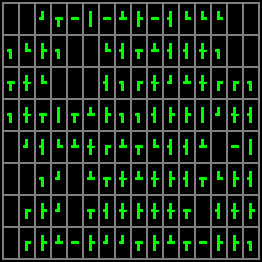
\includegraphics[scale=0.75]{\CURPATH/shuffled.png}
\caption{Разобранная головоломка}
\end{figure}

\dots и собранная:

\begin{figure}[H]
\label{fig:pipe_solved}
\centering
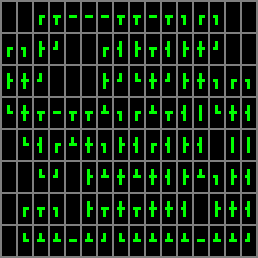
\includegraphics[scale=0.75]{\CURPATH/solved.png}
\caption{Собранная головоломка}
\end{figure}

Попробуем найти способ собрать её.

\subsubsection{Создание}

В начале, нужно её создать.
Вот простая идея.
Возьем массив ячеек 8*16.
Каждая ячейка может содержать какой-то тип блока.
Между ячейками есть стыки:

\pgfmathsetmacro\Width{16}
\pgfmathsetmacro\Height{8}
%\pgfmathsetmacro\Width{10}
%\pgfmathsetmacro\Height{5}
\pgfmathtruncatemacro\WidthMinusI{\Width - 1}
\pgfmathtruncatemacro\WidthMinusII{\Width - 2}
\pgfmathtruncatemacro\HeightMinusI{\Height - 1}
\pgfmathtruncatemacro\HeightMinusII{\Height - 2}
\pgfmathtruncatemacro\HeightPlusII{\Height + 2}
\pgfmathsetmacro\HeightPlusIi{\Height + 1.5}

% see also: http://www.texample.net/tikz/examples/euclid-algorithm/
\begin{center}
\begin{tikzpicture}[set style={{help lines}+=[dashed]},scale=0.7]

	\draw[style=help lines] (0,0) grid +(\Width,\Height);

	\foreach \c in {0,...,\WidthMinusI}
	{
		\foreach \r in {0,...,\HeightMinusII}
			\draw   [red,very thick,-] (\c+0.5,\r+0.75) -- (\c+0.5,\r+1.25);
		%\node[rotate=90] at (\c+0.5,\HeightPlusII) {\Large vjoints[\dots, \c] \normalsize};
		\node[rotate=90] at (\c+0.5,\HeightPlusII) {vjoints[\dots, \c]};
	}

	\foreach \r in {0,...,\HeightMinusI}
	{
		\foreach \c in {0,...,\WidthMinusII}
			\draw   [blue,very thick,-] (\c+0.75,\r+0.5) -- (\c+1.25,\r+0.5);
		\pgfmathtruncatemacro\hjointslabel{\HeightMinusI - \r}
		%\node at (-1.5,\r+0.5) {\large hjoints[\hjointslabel, \dots] \normalsize};
		\node at (-1.5,\r+0.5) {hjoints[\hjointslabel, \dots]};
	}

\end{tikzpicture}
\end{center}



Синие линии это горизонтальные стыки, красные линии это вертикальные стыки.
Мы просто случайно выставляем каждый стык в 0/false (отсутствует) или 1/true (присутствует).

После этого, теперь легко найти тип каждой ячейки.
А это:

\newcommand{\HeaderColor}{\cellcolor{blue!25}}
\begin{center}
\begin{longtable}{ | l | l | l | l | }
\hline
\HeaderColor стыки & \HeaderColor наше внутреннее название & \HeaderColor угол & \HeaderColor символ \\
\hline
0	&type 0		&	0$^{\circ}$	& (пробел)	\\
2	&type 2a	&	0$^{\circ}$	& \pmboxdrawuni{2503} \\ % ┃
2	&type 2a	&	90$^{\circ}$	& \pmboxdrawuni{2501} \\ % ━
2	&type 2b	&	0$^{\circ}$	& \pmboxdrawuni{250F} \\ % ┏
2	&type 2b	&	90$^{\circ}$	& \pmboxdrawuni{2513} \\ % ┓
2	&type 2b	&	180$^{\circ}$	& \pmboxdrawuni{251B} \\ % ┛
2	&type 2b	&	270$^{\circ}$	& \pmboxdrawuni{2517} \\ % ┗
3	&type 3		&	0$^{\circ}$	& \pmboxdrawuni{2523} \\ % ┣
3 	&type 3		&	90$^{\circ}$	& \pmboxdrawuni{2533} \\ % ┳
3	&type 3		&	180$^{\circ}$	& \pmboxdrawuni{252B} \\ % ┫
3	&type 3		&	270$^{\circ}$	& \pmboxdrawuni{253B} \\ % ┻
4	&type 4		&	0$^{\circ}$	& \pmboxdrawuni{254B} \\ % ╋
\hline
\end{longtable}
\end{center}

\textit{Висящие} стыки могут присутствовать на первой стадии (т.е., ячейки только с одним стыком), но они удалются
рекурсивно, и эти ячейки преобразуются в пустые ячейки.
Так что, в самом конце, все ячейки имеют минимум 2 стыка, и вся эта сантехническая система не имеет связей с внешним миром ---
я надеюсь, из-за этого станет немного проще.

Исходник генератора на Си здесь: \url{.../pipe/generator}.
Все вертикальные стыки хранятся в глобальном массиве \textit{hjoints[]} и вертикальные в \textit{vjoints[]}.

Программа на Си генерирует ANSI-раскрашенный вывод, как это было показано выше
(\ref{fig:pipe_shuffled}, \ref{fig:pipe_solved}) плюс массив типов для каждой ячейки, но без информации об углах:

\begin{lstlisting}[label=init_cells]
[
["0", "0", "2b", "3", "2a", "2a", "2a", "3", "3", "2a", "3", "2b", "2b", "2b", "0", "0"],
["2b", "2b", "3", "2b", "0", "0", "2b", "3", "3", "3", "3", "3", "4", "2b", "0", "0"],
["3", "4", "2b", "0", "0", "0", "3", "2b", "2b", "4", "2b", "3", "4", "2b", "2b", "2b"],
["2b", "4", "3", "2a", "3", "3", "3", "2b", "2b", "3", "3", "3", "2a", "2b", "4", "3"],
["0", "2b", "3", "2b", "3", "4", "2b", "3", "3", "2b", "3", "3", "3", "0", "2a", "2a"],
["0", "0", "2b", "2b", "0", "3", "3", "4", "3", "4", "3", "3", "3", "2b", "3", "3"],
["0", "2b", "3", "2b", "0", "3", "3", "4", "3", "4", "4", "3", "0", "3", "4", "3"],
["0", "2b", "3", "3", "2a", "3", "2b", "2b", "3", "3", "3", "3", "2a", "3", "3", "2b"],
]
\end{lstlisting}

\subsubsection{Решение}

Прежде всего, мы будем работать с массивом ячеек 8*16, где каждый элемент имеет 4 бита:
``T'' (top/верх),
``B'' (bottom/низ),
``L'' (left/лево),
``R'' (right/право).
Каждый бит представляет собой половину стыка.

% see also: http://www.texample.net/tikz/examples/euclid-algorithm/
\begin{center}
\begin{tikzpicture}[set style={{help lines}+=[dashed]},scale=0.7]

	\draw[style=help lines] (0,0) grid +(\Width,\Height);
	
	\foreach \c in {0,...,\WidthMinusI}
		%\node[rotate=90] at (\c+0.5,\HeightPlusIi) {\Large [\dots, \c] \normalsize};
		\node[rotate=90] at (\c+0.5,\HeightPlusIi) {[\dots, \c]};
	
	\foreach \r in {0,...,\HeightMinusI}
	{
		\pgfmathtruncatemacro\hlabel{\HeightMinusI - \r}
		%\node at (-1.5,\r+0.5) {\large [\hlabel, \dots] \normalsize};
		\node at (-1.5,\r+0.5) {[\hlabel, \dots]};
	
		\pgfmathsetmacro\Shift{0.325}
		\foreach \c in {0,...,\WidthMinusI}
		{
			\node at (\c+0.5,\r+0.5 + \Shift) {\footnotesize T \normalsize};
			\node at (\c+0.5,\r+0.5 - \Shift) {\footnotesize B \normalsize};
			\node at (\c+0.5 - \Shift,\r+0.5) {\footnotesize L \normalsize};
			\node at (\c+0.5 + \Shift,\r+0.5) {\footnotesize R \normalsize};
		}
	}

\end{tikzpicture}
\end{center}


Теперь определяем массив для каждого из четырех полустыков + информация об угле:

\begin{lstlisting}
HEIGHT=8
WIDTH=16

# if T/B/R/L is Bool instead of Int, Z3 solver will work faster
T=[[Bool('cell_%d_%d_top' % (r, c)) for c in range(WIDTH)] for r in range(HEIGHT)]
B=[[Bool('cell_%d_%d_bottom' % (r, c)) for c in range(WIDTH)] for r in range(HEIGHT)]
R=[[Bool('cell_%d_%d_right' % (r, c)) for c in range(WIDTH)] for r in range(HEIGHT)]
L=[[Bool('cell_%d_%d_left' % (r, c)) for c in range(WIDTH)] for r in range(HEIGHT)]
A=[[Int('cell_%d_%d_angle' % (r, c)) for c in range(WIDTH)] for r in range(HEIGHT)]
\end{lstlisting}

Мы знаем, что если каждый из полустыков присутствует, ответный полустык также должен присутствовать, и наоборот. 
Определяем всё это используя эти констрайнты:

\begin{lstlisting}
# shorthand variables for True and False:
t=True
f=False

# "top" of each cell must be equal to "bottom" of the cell above
# "bottom" of each cell must be equal to "top" of the cell below
# "left" of each cell must be equal to "right" of the cell at left
# "right" of each cell must be equal to "left" of the cell at right
for r in range(HEIGHT):
    for c in range(WIDTH):
        if r!=0:
            s.add(T[r][c]==B[r-1][c])
        if r!=HEIGHT-1:
            s.add(B[r][c]==T[r+1][c])
        if c!=0:
            s.add(L[r][c]==R[r][c-1])
        if c!=WIDTH-1:
            s.add(R[r][c]==L[r][c+1])

# "left" of each cell of first column shouldn't have any connection
# so is "right" of each cell of the last column
for r in range(HEIGHT):
    s.add(L[r][0]==f)
    s.add(R[r][WIDTH-1]==f)

# "top" of each cell of the first row shouldn't have any connection
# so is "bottom" of each cell of the last row
for c in range(WIDTH):
    s.add(T[0][c]==f)
    s.add(B[HEIGHT-1][c]==f)
\end{lstlisting}

Теперь перебираем все ячейки в изначальном массиве (\ref{init_cells}).
Первые две ячейки здесь пустые. И третья имеет тип ``2b''.
Это ``\pmboxdrawuni{250F}'' % ┏
и его можно ориентировать четырьмя разными способами.
И если её угол это 0$^{\circ}$, верхний и правый полустыки присутствуют, остальные отсутствуют.
Если он имеет угол 90$^{\circ}$, он выглядит как 
``\pmboxdrawuni{2513}'', % ┓
и верхник и левый полустыки присутствуют, остальные отсутствуют.

На обычном русском языке: ``если ячейка этого типа имеет угол 0$^{\circ}$, вот эти полустыки должны присутствовать \textbf{ИЛИ}
если она имеет угол 90$^{\circ}$, эти полустыки должны присутствовать, \textbf{ИЛИ}, итд, итд.''

Точно также, мы определяем эти правила для всех типов и всех возможных углов:

\begin{lstlisting}
for r in range(HEIGHT):
    for c in range(WIDTH):
        ty=cells_type[r][c]

        if ty=="0":
            s.add(A[r][c]==f)
            s.add(T[r][c]==f, B[r][c]==f, L[r][c]==f, R[r][c]==f)

        if ty=="2a":
            s.add(Or(And(A[r][c]==0, L[r][c]==f, R[r][c]==f, T[r][c]==t, B[r][c]==t),   # §\pmboxdrawuni{2503}§
                    And(A[r][c]==90, L[r][c]==t, R[r][c]==t, T[r][c]==f, B[r][c]==f)))  # §\pmboxdrawuni{2501}§

        if ty=="2b":
            s.add(Or(And(A[r][c]==0, L[r][c]==f, R[r][c]==t, T[r][c]==f, B[r][c]==t),   # §\pmboxdrawuni{250F}§
                    And(A[r][c]==90, L[r][c]==t, R[r][c]==f, T[r][c]==f, B[r][c]==t),   # §\pmboxdrawuni{2513}§
                    And(A[r][c]==180, L[r][c]==t, R[r][c]==f, T[r][c]==t, B[r][c]==f),  # §\pmboxdrawuni{251B}§
                    And(A[r][c]==270, L[r][c]==f, R[r][c]==t, T[r][c]==t, B[r][c]==f))) # §\pmboxdrawuni{2517}§
	
        if ty=="3":
            s.add(Or(And(A[r][c]==0, L[r][c]==f, R[r][c]==t, T[r][c]==t, B[r][c]==t),   # §\pmboxdrawuni{2523}§
                    And(A[r][c]==90, L[r][c]==t, R[r][c]==t, T[r][c]==f, B[r][c]==t),   # §\pmboxdrawuni{2533}§
                    And(A[r][c]==180, L[r][c]==t, R[r][c]==f, T[r][c]==t, B[r][c]==t),  # §\pmboxdrawuni{252B}§
                    And(A[r][c]==270, L[r][c]==t, R[r][c]==t, T[r][c]==t, B[r][c]==f))) # §\pmboxdrawuni{253B}§

        if ty=="4":
            s.add(A[r][c]==0)
            s.add(T[r][c]==t, B[r][c]==t, L[r][c]==t, R[r][c]==t) # §\pmboxdrawuni{254B}§
\end{lstlisting}

Полный исходник здесь: \url{.../solver/solve_pipe_puzzle1.py}.

Получается такой результат (выводит угол для каждой ячейки и (псевдо)графическое представление):

\begin{figure}[H]
\centering
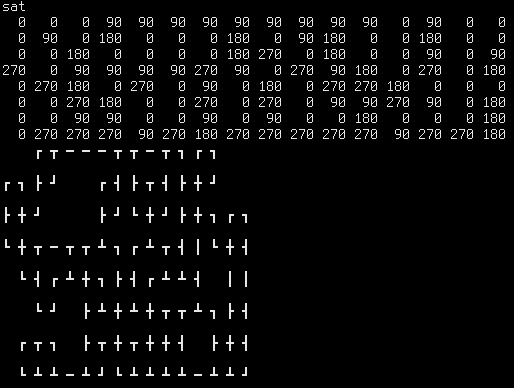
\includegraphics[scale=0.75]{\CURPATH/solver/solver.png}
\caption{Вывод скрипта солвера}
\end{figure}

Это работает $\approx 4$ секунды на моем старом и медленном Intel Atom N455 1.66GHz.
Быстро ли это? Не знаю, но снова вот что действительно круто, это то что мы понятия не имеем о какой-то математической
теории за всем этим, мы просто объявили ячейки, (полу-)стыки и определили отношения между ними.

Теперь следующий вопрос это, сколько здесь возможных решений?
Используя раннее описанный метод (\ref{SMTEnumerate}), я немного изменил скрипт солвера
\footnote{\url{.../solver/solve_pipe_puzzle2.py}} и солвер
сказал что возможно два решения.

Сравним их используя gvimdiff:

\begin{figure}[H]
\centering
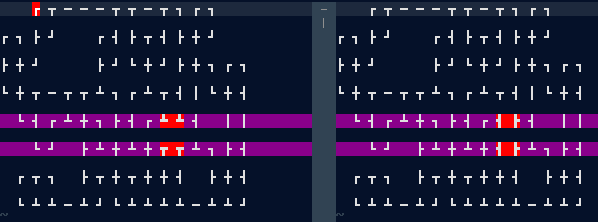
\includegraphics[scale=0.75]{\CURPATH/solver/diff.png}
\caption{Вывод gvimdiff (извините за мой красный курсор в левой части в левом верхнем углу)}
\end{figure}

4 ячейки в середине могут быть ориентированы по-разному.
Видимо, другие головоломки могут также выдавать разные результаты.

P.S.
\textit{Полу-стык} определен как булевый тип.
Но на самом деле, первая версия солвера была написана используя целочисленный тип для полу-стыков,
и 0 использовалось для False и 1 для True.
Я так сделал, потому что хотел более компактный исходный код, без использования длинных слов как ``False'' и ``True''.
И это работало, но медленнее. Вероятно, Z3 работает с булевыми типами быстрее? Лучше?
Так или иначе, я пишу это чтобы отметить, что, если нужно, целочисленный тип можно использовать вместо булевого.


\section{Развлекательная математика и головоломки}

\subsection{Судоку}

Головоломка Судоку это решетка 9*9, некоторые ячейки заполнены значениями, некоторые пустые:

% copypasted from http://www.texample.net/tikz/examples/sudoku/
\newcounter{row}
\newcounter{col}

\newcommand\setrow[9]{
  \setcounter{col}{1}
  \foreach \n in {#1, #2, #3, #4, #5, #6, #7, #8, #9} {
    \edef\x{\value{col} - 0.5}
    \edef\y{9.5 - \value{row}}
    \node[anchor=center] at (\x, \y) {\n};
    \stepcounter{col}
  }
  \stepcounter{row}
}

\begin{center}
\begin{tikzpicture}[scale=.7]
  \begin{scope}
    \draw (0, 0) grid (9, 9);
    \draw[very thick, scale=3] (0, 0) grid (3, 3);

    \setcounter{row}{1}
    \setrow { }{ }{5}  {3}{ }{ }  { }{ }{ }
    \setrow {8}{ }{ }  { }{ }{ }  { }{2}{ }
    \setrow { }{7}{ }  { }{1}{ }  {5}{ }{ }

    \setrow {4}{ }{ }  { }{ }{5}  {3}{ }{ }
    \setrow { }{1}{ }  { }{7}{ }  { }{ }{6}
    \setrow { }{ }{3}  {2}{ }{ }  { }{8}{ }

    \setrow { }{6}{ }  {5}{ }{ }  { }{ }{9}
    \setrow { }{ }{4}  { }{ }{ }  { }{3}{ }
    \setrow { }{ }{ }  { }{ }{9}  {7}{ }{ }

    \node[anchor=center] at (4.5, -0.5) {Нерешенная Судоку};
  \end{scope}
\end{tikzpicture}
\end{center}

Числа в каждом ряду должны быть уникальными, т.е., каждый ряд должен содержать 9 чисел в пределах 1..9 без повторений.
Та же история и для каждого столбца и каждого квадрата 3*3.

Головоломка представляет собой хороший кандидат, на котором можно попробовать \ac{SMT}-солвер, потому что это,
в общем-то, просто нерешенная система уравнений.

\input{puzzles/sudoku/1/main_RU}
%\input{puzzles/sudoku/GT/main_RU}
%\input{puzzles/sudoku/killer/main_RU}
\input{puzzles/sudoku/KLEE/main_RU}
\input{puzzles/sudoku/SAT/main_RU}


\subsection{Головоломка зебры (\ac{AKA} Загадка Эйнштейна)}

\input{puzzles/zebra/SMT/main_RU}
\input{puzzles/zebra/KLEE/main_RU}
\input{puzzles/zebra/SAT/main_RU}


\subsection{Решение головоломки ``трубы'' используя Z3 SMT-солвер}

\renewcommand{\CURPATH}{puzzles/pipe}

Головоломка ``трубы'' это популярная головоломка (просто погуглите ``pipe puzzle'' и посмотрите на картинки).

Вот как выглядит головоломка в разобранном виде:

\begin{figure}[H]
\label{fig:pipe_shuffled}
\centering
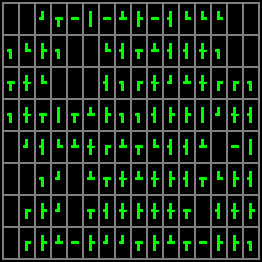
\includegraphics[scale=0.75]{\CURPATH/shuffled.png}
\caption{Разобранная головоломка}
\end{figure}

\dots и собранная:

\begin{figure}[H]
\label{fig:pipe_solved}
\centering
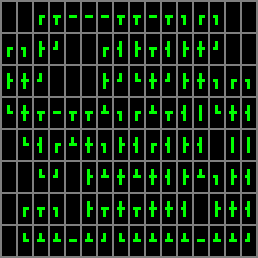
\includegraphics[scale=0.75]{\CURPATH/solved.png}
\caption{Собранная головоломка}
\end{figure}

Попробуем найти способ собрать её.

\subsubsection{Создание}

В начале, нужно её создать.
Вот простая идея.
Возьем массив ячеек 8*16.
Каждая ячейка может содержать какой-то тип блока.
Между ячейками есть стыки:

\input{\CURPATH/pipe_gen.tex}

Синие линии это горизонтальные стыки, красные линии это вертикальные стыки.
Мы просто случайно выставляем каждый стык в 0/false (отсутствует) или 1/true (присутствует).

После этого, теперь легко найти тип каждой ячейки.
А это:

\newcommand{\HeaderColor}{\cellcolor{blue!25}}
\begin{center}
\begin{longtable}{ | l | l | l | l | }
\hline
\HeaderColor стыки & \HeaderColor наше внутреннее название & \HeaderColor угол & \HeaderColor символ \\
\hline
0	&type 0		&	0$^{\circ}$	& (пробел)	\\
2	&type 2a	&	0$^{\circ}$	& \pmboxdrawuni{2503} \\ % ┃
2	&type 2a	&	90$^{\circ}$	& \pmboxdrawuni{2501} \\ % ━
2	&type 2b	&	0$^{\circ}$	& \pmboxdrawuni{250F} \\ % ┏
2	&type 2b	&	90$^{\circ}$	& \pmboxdrawuni{2513} \\ % ┓
2	&type 2b	&	180$^{\circ}$	& \pmboxdrawuni{251B} \\ % ┛
2	&type 2b	&	270$^{\circ}$	& \pmboxdrawuni{2517} \\ % ┗
3	&type 3		&	0$^{\circ}$	& \pmboxdrawuni{2523} \\ % ┣
3 	&type 3		&	90$^{\circ}$	& \pmboxdrawuni{2533} \\ % ┳
3	&type 3		&	180$^{\circ}$	& \pmboxdrawuni{252B} \\ % ┫
3	&type 3		&	270$^{\circ}$	& \pmboxdrawuni{253B} \\ % ┻
4	&type 4		&	0$^{\circ}$	& \pmboxdrawuni{254B} \\ % ╋
\hline
\end{longtable}
\end{center}

\textit{Висящие} стыки могут присутствовать на первой стадии (т.е., ячейки только с одним стыком), но они удалются
рекурсивно, и эти ячейки преобразуются в пустые ячейки.
Так что, в самом конце, все ячейки имеют минимум 2 стыка, и вся эта сантехническая система не имеет связей с внешним миром ---
я надеюсь, из-за этого станет немного проще.

Исходник генератора на Си здесь: \url{.../pipe/generator}.
Все вертикальные стыки хранятся в глобальном массиве \textit{hjoints[]} и вертикальные в \textit{vjoints[]}.

Программа на Си генерирует ANSI-раскрашенный вывод, как это было показано выше
(\ref{fig:pipe_shuffled}, \ref{fig:pipe_solved}) плюс массив типов для каждой ячейки, но без информации об углах:

\begin{lstlisting}[label=init_cells]
[
["0", "0", "2b", "3", "2a", "2a", "2a", "3", "3", "2a", "3", "2b", "2b", "2b", "0", "0"],
["2b", "2b", "3", "2b", "0", "0", "2b", "3", "3", "3", "3", "3", "4", "2b", "0", "0"],
["3", "4", "2b", "0", "0", "0", "3", "2b", "2b", "4", "2b", "3", "4", "2b", "2b", "2b"],
["2b", "4", "3", "2a", "3", "3", "3", "2b", "2b", "3", "3", "3", "2a", "2b", "4", "3"],
["0", "2b", "3", "2b", "3", "4", "2b", "3", "3", "2b", "3", "3", "3", "0", "2a", "2a"],
["0", "0", "2b", "2b", "0", "3", "3", "4", "3", "4", "3", "3", "3", "2b", "3", "3"],
["0", "2b", "3", "2b", "0", "3", "3", "4", "3", "4", "4", "3", "0", "3", "4", "3"],
["0", "2b", "3", "3", "2a", "3", "2b", "2b", "3", "3", "3", "3", "2a", "3", "3", "2b"],
]
\end{lstlisting}

\subsubsection{Решение}

Прежде всего, мы будем работать с массивом ячеек 8*16, где каждый элемент имеет 4 бита:
``T'' (top/верх),
``B'' (bottom/низ),
``L'' (left/лево),
``R'' (right/право).
Каждый бит представляет собой половину стыка.

\input{\CURPATH/pipe_solve.tex}

Теперь определяем массив для каждого из четырех полустыков + информация об угле:

\begin{lstlisting}
HEIGHT=8
WIDTH=16

# if T/B/R/L is Bool instead of Int, Z3 solver will work faster
T=[[Bool('cell_%d_%d_top' % (r, c)) for c in range(WIDTH)] for r in range(HEIGHT)]
B=[[Bool('cell_%d_%d_bottom' % (r, c)) for c in range(WIDTH)] for r in range(HEIGHT)]
R=[[Bool('cell_%d_%d_right' % (r, c)) for c in range(WIDTH)] for r in range(HEIGHT)]
L=[[Bool('cell_%d_%d_left' % (r, c)) for c in range(WIDTH)] for r in range(HEIGHT)]
A=[[Int('cell_%d_%d_angle' % (r, c)) for c in range(WIDTH)] for r in range(HEIGHT)]
\end{lstlisting}

Мы знаем, что если каждый из полустыков присутствует, ответный полустык также должен присутствовать, и наоборот. 
Определяем всё это используя эти констрайнты:

\begin{lstlisting}
# shorthand variables for True and False:
t=True
f=False

# "top" of each cell must be equal to "bottom" of the cell above
# "bottom" of each cell must be equal to "top" of the cell below
# "left" of each cell must be equal to "right" of the cell at left
# "right" of each cell must be equal to "left" of the cell at right
for r in range(HEIGHT):
    for c in range(WIDTH):
        if r!=0:
            s.add(T[r][c]==B[r-1][c])
        if r!=HEIGHT-1:
            s.add(B[r][c]==T[r+1][c])
        if c!=0:
            s.add(L[r][c]==R[r][c-1])
        if c!=WIDTH-1:
            s.add(R[r][c]==L[r][c+1])

# "left" of each cell of first column shouldn't have any connection
# so is "right" of each cell of the last column
for r in range(HEIGHT):
    s.add(L[r][0]==f)
    s.add(R[r][WIDTH-1]==f)

# "top" of each cell of the first row shouldn't have any connection
# so is "bottom" of each cell of the last row
for c in range(WIDTH):
    s.add(T[0][c]==f)
    s.add(B[HEIGHT-1][c]==f)
\end{lstlisting}

Теперь перебираем все ячейки в изначальном массиве (\ref{init_cells}).
Первые две ячейки здесь пустые. И третья имеет тип ``2b''.
Это ``\pmboxdrawuni{250F}'' % ┏
и его можно ориентировать четырьмя разными способами.
И если её угол это 0$^{\circ}$, верхний и правый полустыки присутствуют, остальные отсутствуют.
Если он имеет угол 90$^{\circ}$, он выглядит как 
``\pmboxdrawuni{2513}'', % ┓
и верхник и левый полустыки присутствуют, остальные отсутствуют.

На обычном русском языке: ``если ячейка этого типа имеет угол 0$^{\circ}$, вот эти полустыки должны присутствовать \textbf{ИЛИ}
если она имеет угол 90$^{\circ}$, эти полустыки должны присутствовать, \textbf{ИЛИ}, итд, итд.''

Точно также, мы определяем эти правила для всех типов и всех возможных углов:

\begin{lstlisting}
for r in range(HEIGHT):
    for c in range(WIDTH):
        ty=cells_type[r][c]

        if ty=="0":
            s.add(A[r][c]==f)
            s.add(T[r][c]==f, B[r][c]==f, L[r][c]==f, R[r][c]==f)

        if ty=="2a":
            s.add(Or(And(A[r][c]==0, L[r][c]==f, R[r][c]==f, T[r][c]==t, B[r][c]==t),   # §\pmboxdrawuni{2503}§
                    And(A[r][c]==90, L[r][c]==t, R[r][c]==t, T[r][c]==f, B[r][c]==f)))  # §\pmboxdrawuni{2501}§

        if ty=="2b":
            s.add(Or(And(A[r][c]==0, L[r][c]==f, R[r][c]==t, T[r][c]==f, B[r][c]==t),   # §\pmboxdrawuni{250F}§
                    And(A[r][c]==90, L[r][c]==t, R[r][c]==f, T[r][c]==f, B[r][c]==t),   # §\pmboxdrawuni{2513}§
                    And(A[r][c]==180, L[r][c]==t, R[r][c]==f, T[r][c]==t, B[r][c]==f),  # §\pmboxdrawuni{251B}§
                    And(A[r][c]==270, L[r][c]==f, R[r][c]==t, T[r][c]==t, B[r][c]==f))) # §\pmboxdrawuni{2517}§
	
        if ty=="3":
            s.add(Or(And(A[r][c]==0, L[r][c]==f, R[r][c]==t, T[r][c]==t, B[r][c]==t),   # §\pmboxdrawuni{2523}§
                    And(A[r][c]==90, L[r][c]==t, R[r][c]==t, T[r][c]==f, B[r][c]==t),   # §\pmboxdrawuni{2533}§
                    And(A[r][c]==180, L[r][c]==t, R[r][c]==f, T[r][c]==t, B[r][c]==t),  # §\pmboxdrawuni{252B}§
                    And(A[r][c]==270, L[r][c]==t, R[r][c]==t, T[r][c]==t, B[r][c]==f))) # §\pmboxdrawuni{253B}§

        if ty=="4":
            s.add(A[r][c]==0)
            s.add(T[r][c]==t, B[r][c]==t, L[r][c]==t, R[r][c]==t) # §\pmboxdrawuni{254B}§
\end{lstlisting}

Полный исходник здесь: \url{.../solver/solve_pipe_puzzle1.py}.

Получается такой результат (выводит угол для каждой ячейки и (псевдо)графическое представление):

\begin{figure}[H]
\centering
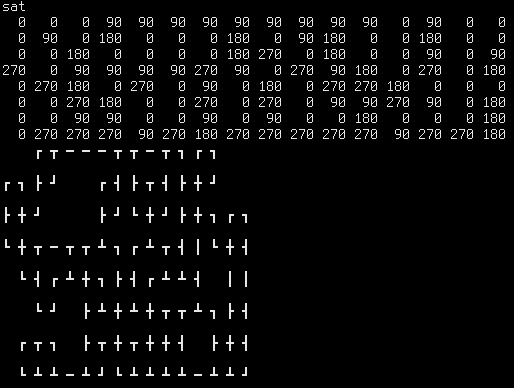
\includegraphics[scale=0.75]{\CURPATH/solver/solver.png}
\caption{Вывод скрипта солвера}
\end{figure}

Это работает $\approx 4$ секунды на моем старом и медленном Intel Atom N455 1.66GHz.
Быстро ли это? Не знаю, но снова вот что действительно круто, это то что мы понятия не имеем о какой-то математической
теории за всем этим, мы просто объявили ячейки, (полу-)стыки и определили отношения между ними.

Теперь следующий вопрос это, сколько здесь возможных решений?
Используя раннее описанный метод (\ref{SMTEnumerate}), я немного изменил скрипт солвера
\footnote{\url{.../solver/solve_pipe_puzzle2.py}} и солвер
сказал что возможно два решения.

Сравним их используя gvimdiff:

\begin{figure}[H]
\centering
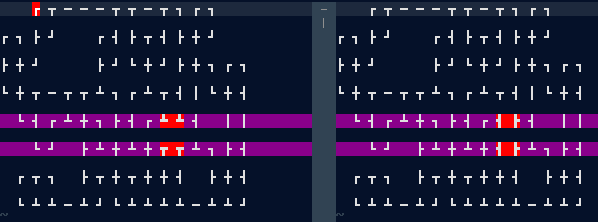
\includegraphics[scale=0.75]{\CURPATH/solver/diff.png}
\caption{Вывод gvimdiff (извините за мой красный курсор в левой части в левом верхнем углу)}
\end{figure}

4 ячейки в середине могут быть ориентированы по-разному.
Видимо, другие головоломки могут также выдавать разные результаты.

P.S.
\textit{Полу-стык} определен как булевый тип.
Но на самом деле, первая версия солвера была написана используя целочисленный тип для полу-стыков,
и 0 использовалось для False и 1 для True.
Я так сделал, потому что хотел более компактный исходный код, без использования длинных слов как ``False'' и ``True''.
И это работало, но медленнее. Вероятно, Z3 работает с булевыми типами быстрее? Лучше?
Так или иначе, я пишу это чтобы отметить, что, если нужно, целочисленный тип можно использовать вместо булевого.


\section{Развлекательная математика и головоломки}

\input{puzzles/sudoku/main_RU}
\input{puzzles/zebra/main_RU}
\input{puzzles/pipe/main_RU}
\input{puzzles/rubik2/failed_SMT/main_RU}
\input{puzzles/rubik2/SAT/main_RU}
\input{puzzles/rubik3/one_face_SMT/main_RU}
%\input{puzzles/numberlink/main_RU}
%\input{puzzles/two_parks_RU}
\input{puzzles/alphametics/main_RU}
%\input{puzzles/2015_AIME_II_Problems_12_RU}
%\input{puzzles/fred/main_RU}
%\input{puzzles/MC/main_RU}
%\input{puzzles/coin_flip/main_RU}
%\input{puzzles/Mock_AIME_2_2006-2007_Problem_8_RU}
%\input{puzzles/2012_AIME_I_Problems_1_RU}
%\input{puzzles/keypad_RU}


\section{Развлекательная математика и головоломки}

\input{puzzles/sudoku/main_RU}
\input{puzzles/zebra/main_RU}
\input{puzzles/pipe/main_RU}
\input{puzzles/rubik2/failed_SMT/main_RU}
\input{puzzles/rubik2/SAT/main_RU}
\input{puzzles/rubik3/one_face_SMT/main_RU}
%\input{puzzles/numberlink/main_RU}
%\input{puzzles/two_parks_RU}
\input{puzzles/alphametics/main_RU}
%\input{puzzles/2015_AIME_II_Problems_12_RU}
%\input{puzzles/fred/main_RU}
%\input{puzzles/MC/main_RU}
%\input{puzzles/coin_flip/main_RU}
%\input{puzzles/Mock_AIME_2_2006-2007_Problem_8_RU}
%\input{puzzles/2012_AIME_I_Problems_1_RU}
%\input{puzzles/keypad_RU}


\section{Развлекательная математика и головоломки}

\input{puzzles/sudoku/main_RU}
\input{puzzles/zebra/main_RU}
\input{puzzles/pipe/main_RU}
\input{puzzles/rubik2/failed_SMT/main_RU}
\input{puzzles/rubik2/SAT/main_RU}
\input{puzzles/rubik3/one_face_SMT/main_RU}
%\input{puzzles/numberlink/main_RU}
%\input{puzzles/two_parks_RU}
\input{puzzles/alphametics/main_RU}
%\input{puzzles/2015_AIME_II_Problems_12_RU}
%\input{puzzles/fred/main_RU}
%\input{puzzles/MC/main_RU}
%\input{puzzles/coin_flip/main_RU}
%\input{puzzles/Mock_AIME_2_2006-2007_Problem_8_RU}
%\input{puzzles/2012_AIME_I_Problems_1_RU}
%\input{puzzles/keypad_RU}


%\section{Развлекательная математика и головоломки}

\input{puzzles/sudoku/main_RU}
\input{puzzles/zebra/main_RU}
\input{puzzles/pipe/main_RU}
\input{puzzles/rubik2/failed_SMT/main_RU}
\input{puzzles/rubik2/SAT/main_RU}
\input{puzzles/rubik3/one_face_SMT/main_RU}
%\input{puzzles/numberlink/main_RU}
%\input{puzzles/two_parks_RU}
\input{puzzles/alphametics/main_RU}
%\input{puzzles/2015_AIME_II_Problems_12_RU}
%\input{puzzles/fred/main_RU}
%\input{puzzles/MC/main_RU}
%\input{puzzles/coin_flip/main_RU}
%\input{puzzles/Mock_AIME_2_2006-2007_Problem_8_RU}
%\input{puzzles/2012_AIME_I_Problems_1_RU}
%\input{puzzles/keypad_RU}


%\input{puzzles/two_parks_RU}
\subsection{Альфаметика}

Согласно Дональду Кнуту, термин ``Альфаметика'' был придуман Дж. Эйч. Аш. Хантером.
Это головоломка: какие десятичные цифры в пределах 0..9 нужно присвоить каждой букве, чтобы это уравнение было справедливо?

\begin{lstlisting}
  SEND
+ MORE
 -----
 MONEY
\end{lstlisting}

Для Z3 это легко:

\lstinputlisting{puzzles/alphametics/alpha.py}

Вывод:

\begin{lstlisting}
sat
[E, = 5,
 S, = 9,
 M, = 1,
 N, = 6,
 D, = 7,
 R, = 8,
 O, = 0,
 Y = 2]
\end{lstlisting}

Вот еще одна, из \ac{TAOCP} том IV (\url{http://www-cs-faculty.stanford.edu/~uno/fasc2b.ps.gz}):

\lstinputlisting{puzzles/alphametics/alpha2.py}

\begin{lstlisting}
sat
[L, = 6,
 S, = 7,
 N, = 2,
 T, = 1,
 I, = 5,
 V = 3,
 A, = 8,
 R, = 9,
 O, = 4,
 TRIO = 1954,
 SONATA, = 742818,
 VIOLA, = 35468,
 VIOLIN, = 354652]
\end{lstlisting}

% TODO URL
Эту головоломку я нашел в примерах pySMT:

\lstinputlisting{puzzles/alphametics/alpha3.py}

\begin{lstlisting}
sat
[D = 5, R = 4, O = 3, E = 8, L = 6, W = 7, H = 2]
\end{lstlisting}

%%% 

Это упражнение Q209 из
[Companion to the Papers of Donald Knuth]\footnote{\url{http://www-cs-faculty.stanford.edu/~knuth/cp.html}}.

\begin{lstlisting}
 KNIFE
  FORK
 SPOON
  SOUP
------
SUPPER
\end{lstlisting}

В целях упрощения, я добавил ф-цию (list\_to\_expr()):

\lstinputlisting{puzzles/alphametics/alpha4.py}

\begin{lstlisting}
sat
[K = 7,
 N = 4,
 R = 9,
 I = 1,
 E = 6,
 S = 0,
 O = 3,
 F = 5,
 U = 8,
 P = 2,
 SUPPER = 82269,
 SOUP = 382,
 SPOON = 2334,
 FORK = 5397,
 KNIFE = 74156]
\end{lstlisting}

S это 0, так что значение SUPPER начинается с (убранного) нуля. Скажем так, нам это не нравится.
Добавим это, чтобы это исправить:

\begin{lstlisting}
s.add(S!=0)
\end{lstlisting}

\begin{lstlisting}
sat
[K = 8,
 N = 4,
 R = 3,
 I = 7,
 E = 6,
 S = 1,
 O = 9,
 F = 2,
 U = 0,
 P = 5,
 SUPPER = 105563,
 SOUP = 1905,
 SPOON = 15994,
 FORK = 2938,
 KNIFE = 84726]
\end{lstlisting}

\paragraph{Создание своей собственной головоломки}

Вот проблема: есть только 10 букв, но как их выбрать из числа слов?
Мы можем использовать Z3 для этого:

\lstinputlisting{puzzles/alphametics/gen.py}

Это первая сгенерированная головоломка:

\begin{lstlisting}
sat
EGGS
JELLY
LUNCH
C 5
E 6
G 3
H 7
J 0
L 1
N 4
S 8
U 2
Y 9
\end{lstlisting}

Что если мы хотим, чтобы слово ``CAKE'' присутствовало в числе ``слагаемых''?

Добавим это:

\begin{lstlisting}
s.add(word_used[words.index('CAKE')])
\end{lstlisting}

\begin{lstlisting}
sat
CAKE
TEA
LUNCH
A 8
C 3
E 1
H 9
J 6
K 2
L 0
N 5
T 7
U 4
\end{lstlisting}

Добавим это:

\begin{lstlisting}
s.add(word_used[words.index('EGGS')])
\end{lstlisting}

Теперь оно может найти пару к EGGS:

\begin{lstlisting}
sat
EGGS
HONEY
LUNCH
C 6
E 7
G 9
H 4
L 5
N 8
O 2
S 3
U 0
Y 1
\end{lstlisting}

\paragraph{Файлы}

\url{https://github.com/DennisYurichev/...}




%\input{puzzles/2015_AIME_II_Problems_12_RU}
%\section{Развлекательная математика и головоломки}

\input{puzzles/sudoku/main_RU}
\input{puzzles/zebra/main_RU}
\input{puzzles/pipe/main_RU}
\input{puzzles/rubik2/failed_SMT/main_RU}
\input{puzzles/rubik2/SAT/main_RU}
\input{puzzles/rubik3/one_face_SMT/main_RU}
%\input{puzzles/numberlink/main_RU}
%\input{puzzles/two_parks_RU}
\input{puzzles/alphametics/main_RU}
%\input{puzzles/2015_AIME_II_Problems_12_RU}
%\input{puzzles/fred/main_RU}
%\input{puzzles/MC/main_RU}
%\input{puzzles/coin_flip/main_RU}
%\input{puzzles/Mock_AIME_2_2006-2007_Problem_8_RU}
%\input{puzzles/2012_AIME_I_Problems_1_RU}
%\input{puzzles/keypad_RU}


%\section{Развлекательная математика и головоломки}

\input{puzzles/sudoku/main_RU}
\input{puzzles/zebra/main_RU}
\input{puzzles/pipe/main_RU}
\input{puzzles/rubik2/failed_SMT/main_RU}
\input{puzzles/rubik2/SAT/main_RU}
\input{puzzles/rubik3/one_face_SMT/main_RU}
%\input{puzzles/numberlink/main_RU}
%\input{puzzles/two_parks_RU}
\input{puzzles/alphametics/main_RU}
%\input{puzzles/2015_AIME_II_Problems_12_RU}
%\input{puzzles/fred/main_RU}
%\input{puzzles/MC/main_RU}
%\input{puzzles/coin_flip/main_RU}
%\input{puzzles/Mock_AIME_2_2006-2007_Problem_8_RU}
%\input{puzzles/2012_AIME_I_Problems_1_RU}
%\input{puzzles/keypad_RU}


%\section{Развлекательная математика и головоломки}

\input{puzzles/sudoku/main_RU}
\input{puzzles/zebra/main_RU}
\input{puzzles/pipe/main_RU}
\input{puzzles/rubik2/failed_SMT/main_RU}
\input{puzzles/rubik2/SAT/main_RU}
\input{puzzles/rubik3/one_face_SMT/main_RU}
%\input{puzzles/numberlink/main_RU}
%\input{puzzles/two_parks_RU}
\input{puzzles/alphametics/main_RU}
%\input{puzzles/2015_AIME_II_Problems_12_RU}
%\input{puzzles/fred/main_RU}
%\input{puzzles/MC/main_RU}
%\input{puzzles/coin_flip/main_RU}
%\input{puzzles/Mock_AIME_2_2006-2007_Problem_8_RU}
%\input{puzzles/2012_AIME_I_Problems_1_RU}
%\input{puzzles/keypad_RU}


%\input{puzzles/Mock_AIME_2_2006-2007_Problem_8_RU}
%\input{puzzles/2012_AIME_I_Problems_1_RU}
%\input{puzzles/keypad_RU}


\section{Развлекательная математика и головоломки}

\subsection{Судоку}

Головоломка Судоку это решетка 9*9, некоторые ячейки заполнены значениями, некоторые пустые:

% copypasted from http://www.texample.net/tikz/examples/sudoku/
\newcounter{row}
\newcounter{col}

\newcommand\setrow[9]{
  \setcounter{col}{1}
  \foreach \n in {#1, #2, #3, #4, #5, #6, #7, #8, #9} {
    \edef\x{\value{col} - 0.5}
    \edef\y{9.5 - \value{row}}
    \node[anchor=center] at (\x, \y) {\n};
    \stepcounter{col}
  }
  \stepcounter{row}
}

\begin{center}
\begin{tikzpicture}[scale=.7]
  \begin{scope}
    \draw (0, 0) grid (9, 9);
    \draw[very thick, scale=3] (0, 0) grid (3, 3);

    \setcounter{row}{1}
    \setrow { }{ }{5}  {3}{ }{ }  { }{ }{ }
    \setrow {8}{ }{ }  { }{ }{ }  { }{2}{ }
    \setrow { }{7}{ }  { }{1}{ }  {5}{ }{ }

    \setrow {4}{ }{ }  { }{ }{5}  {3}{ }{ }
    \setrow { }{1}{ }  { }{7}{ }  { }{ }{6}
    \setrow { }{ }{3}  {2}{ }{ }  { }{8}{ }

    \setrow { }{6}{ }  {5}{ }{ }  { }{ }{9}
    \setrow { }{ }{4}  { }{ }{ }  { }{3}{ }
    \setrow { }{ }{ }  { }{ }{9}  {7}{ }{ }

    \node[anchor=center] at (4.5, -0.5) {Нерешенная Судоку};
  \end{scope}
\end{tikzpicture}
\end{center}

Числа в каждом ряду должны быть уникальными, т.е., каждый ряд должен содержать 9 чисел в пределах 1..9 без повторений.
Та же история и для каждого столбца и каждого квадрата 3*3.

Головоломка представляет собой хороший кандидат, на котором можно попробовать \ac{SMT}-солвер, потому что это,
в общем-то, просто нерешенная система уравнений.

\input{puzzles/sudoku/1/main_RU}
%\input{puzzles/sudoku/GT/main_RU}
%\input{puzzles/sudoku/killer/main_RU}
\input{puzzles/sudoku/KLEE/main_RU}
\input{puzzles/sudoku/SAT/main_RU}


\subsection{Головоломка зебры (\ac{AKA} Загадка Эйнштейна)}

\input{puzzles/zebra/SMT/main_RU}
\input{puzzles/zebra/KLEE/main_RU}
\input{puzzles/zebra/SAT/main_RU}


\subsection{Решение головоломки ``трубы'' используя Z3 SMT-солвер}

\renewcommand{\CURPATH}{puzzles/pipe}

Головоломка ``трубы'' это популярная головоломка (просто погуглите ``pipe puzzle'' и посмотрите на картинки).

Вот как выглядит головоломка в разобранном виде:

\begin{figure}[H]
\label{fig:pipe_shuffled}
\centering
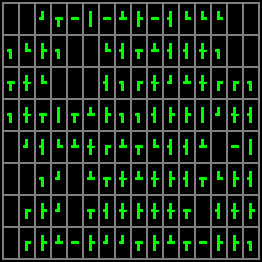
\includegraphics[scale=0.75]{\CURPATH/shuffled.png}
\caption{Разобранная головоломка}
\end{figure}

\dots и собранная:

\begin{figure}[H]
\label{fig:pipe_solved}
\centering
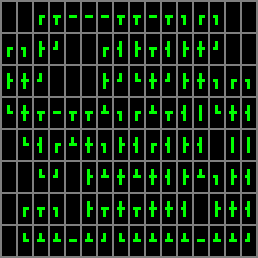
\includegraphics[scale=0.75]{\CURPATH/solved.png}
\caption{Собранная головоломка}
\end{figure}

Попробуем найти способ собрать её.

\subsubsection{Создание}

В начале, нужно её создать.
Вот простая идея.
Возьем массив ячеек 8*16.
Каждая ячейка может содержать какой-то тип блока.
Между ячейками есть стыки:

\input{\CURPATH/pipe_gen.tex}

Синие линии это горизонтальные стыки, красные линии это вертикальные стыки.
Мы просто случайно выставляем каждый стык в 0/false (отсутствует) или 1/true (присутствует).

После этого, теперь легко найти тип каждой ячейки.
А это:

\newcommand{\HeaderColor}{\cellcolor{blue!25}}
\begin{center}
\begin{longtable}{ | l | l | l | l | }
\hline
\HeaderColor стыки & \HeaderColor наше внутреннее название & \HeaderColor угол & \HeaderColor символ \\
\hline
0	&type 0		&	0$^{\circ}$	& (пробел)	\\
2	&type 2a	&	0$^{\circ}$	& \pmboxdrawuni{2503} \\ % ┃
2	&type 2a	&	90$^{\circ}$	& \pmboxdrawuni{2501} \\ % ━
2	&type 2b	&	0$^{\circ}$	& \pmboxdrawuni{250F} \\ % ┏
2	&type 2b	&	90$^{\circ}$	& \pmboxdrawuni{2513} \\ % ┓
2	&type 2b	&	180$^{\circ}$	& \pmboxdrawuni{251B} \\ % ┛
2	&type 2b	&	270$^{\circ}$	& \pmboxdrawuni{2517} \\ % ┗
3	&type 3		&	0$^{\circ}$	& \pmboxdrawuni{2523} \\ % ┣
3 	&type 3		&	90$^{\circ}$	& \pmboxdrawuni{2533} \\ % ┳
3	&type 3		&	180$^{\circ}$	& \pmboxdrawuni{252B} \\ % ┫
3	&type 3		&	270$^{\circ}$	& \pmboxdrawuni{253B} \\ % ┻
4	&type 4		&	0$^{\circ}$	& \pmboxdrawuni{254B} \\ % ╋
\hline
\end{longtable}
\end{center}

\textit{Висящие} стыки могут присутствовать на первой стадии (т.е., ячейки только с одним стыком), но они удалются
рекурсивно, и эти ячейки преобразуются в пустые ячейки.
Так что, в самом конце, все ячейки имеют минимум 2 стыка, и вся эта сантехническая система не имеет связей с внешним миром ---
я надеюсь, из-за этого станет немного проще.

Исходник генератора на Си здесь: \url{.../pipe/generator}.
Все вертикальные стыки хранятся в глобальном массиве \textit{hjoints[]} и вертикальные в \textit{vjoints[]}.

Программа на Си генерирует ANSI-раскрашенный вывод, как это было показано выше
(\ref{fig:pipe_shuffled}, \ref{fig:pipe_solved}) плюс массив типов для каждой ячейки, но без информации об углах:

\begin{lstlisting}[label=init_cells]
[
["0", "0", "2b", "3", "2a", "2a", "2a", "3", "3", "2a", "3", "2b", "2b", "2b", "0", "0"],
["2b", "2b", "3", "2b", "0", "0", "2b", "3", "3", "3", "3", "3", "4", "2b", "0", "0"],
["3", "4", "2b", "0", "0", "0", "3", "2b", "2b", "4", "2b", "3", "4", "2b", "2b", "2b"],
["2b", "4", "3", "2a", "3", "3", "3", "2b", "2b", "3", "3", "3", "2a", "2b", "4", "3"],
["0", "2b", "3", "2b", "3", "4", "2b", "3", "3", "2b", "3", "3", "3", "0", "2a", "2a"],
["0", "0", "2b", "2b", "0", "3", "3", "4", "3", "4", "3", "3", "3", "2b", "3", "3"],
["0", "2b", "3", "2b", "0", "3", "3", "4", "3", "4", "4", "3", "0", "3", "4", "3"],
["0", "2b", "3", "3", "2a", "3", "2b", "2b", "3", "3", "3", "3", "2a", "3", "3", "2b"],
]
\end{lstlisting}

\subsubsection{Решение}

Прежде всего, мы будем работать с массивом ячеек 8*16, где каждый элемент имеет 4 бита:
``T'' (top/верх),
``B'' (bottom/низ),
``L'' (left/лево),
``R'' (right/право).
Каждый бит представляет собой половину стыка.

\input{\CURPATH/pipe_solve.tex}

Теперь определяем массив для каждого из четырех полустыков + информация об угле:

\begin{lstlisting}
HEIGHT=8
WIDTH=16

# if T/B/R/L is Bool instead of Int, Z3 solver will work faster
T=[[Bool('cell_%d_%d_top' % (r, c)) for c in range(WIDTH)] for r in range(HEIGHT)]
B=[[Bool('cell_%d_%d_bottom' % (r, c)) for c in range(WIDTH)] for r in range(HEIGHT)]
R=[[Bool('cell_%d_%d_right' % (r, c)) for c in range(WIDTH)] for r in range(HEIGHT)]
L=[[Bool('cell_%d_%d_left' % (r, c)) for c in range(WIDTH)] for r in range(HEIGHT)]
A=[[Int('cell_%d_%d_angle' % (r, c)) for c in range(WIDTH)] for r in range(HEIGHT)]
\end{lstlisting}

Мы знаем, что если каждый из полустыков присутствует, ответный полустык также должен присутствовать, и наоборот. 
Определяем всё это используя эти констрайнты:

\begin{lstlisting}
# shorthand variables for True and False:
t=True
f=False

# "top" of each cell must be equal to "bottom" of the cell above
# "bottom" of each cell must be equal to "top" of the cell below
# "left" of each cell must be equal to "right" of the cell at left
# "right" of each cell must be equal to "left" of the cell at right
for r in range(HEIGHT):
    for c in range(WIDTH):
        if r!=0:
            s.add(T[r][c]==B[r-1][c])
        if r!=HEIGHT-1:
            s.add(B[r][c]==T[r+1][c])
        if c!=0:
            s.add(L[r][c]==R[r][c-1])
        if c!=WIDTH-1:
            s.add(R[r][c]==L[r][c+1])

# "left" of each cell of first column shouldn't have any connection
# so is "right" of each cell of the last column
for r in range(HEIGHT):
    s.add(L[r][0]==f)
    s.add(R[r][WIDTH-1]==f)

# "top" of each cell of the first row shouldn't have any connection
# so is "bottom" of each cell of the last row
for c in range(WIDTH):
    s.add(T[0][c]==f)
    s.add(B[HEIGHT-1][c]==f)
\end{lstlisting}

Теперь перебираем все ячейки в изначальном массиве (\ref{init_cells}).
Первые две ячейки здесь пустые. И третья имеет тип ``2b''.
Это ``\pmboxdrawuni{250F}'' % ┏
и его можно ориентировать четырьмя разными способами.
И если её угол это 0$^{\circ}$, верхний и правый полустыки присутствуют, остальные отсутствуют.
Если он имеет угол 90$^{\circ}$, он выглядит как 
``\pmboxdrawuni{2513}'', % ┓
и верхник и левый полустыки присутствуют, остальные отсутствуют.

На обычном русском языке: ``если ячейка этого типа имеет угол 0$^{\circ}$, вот эти полустыки должны присутствовать \textbf{ИЛИ}
если она имеет угол 90$^{\circ}$, эти полустыки должны присутствовать, \textbf{ИЛИ}, итд, итд.''

Точно также, мы определяем эти правила для всех типов и всех возможных углов:

\begin{lstlisting}
for r in range(HEIGHT):
    for c in range(WIDTH):
        ty=cells_type[r][c]

        if ty=="0":
            s.add(A[r][c]==f)
            s.add(T[r][c]==f, B[r][c]==f, L[r][c]==f, R[r][c]==f)

        if ty=="2a":
            s.add(Or(And(A[r][c]==0, L[r][c]==f, R[r][c]==f, T[r][c]==t, B[r][c]==t),   # §\pmboxdrawuni{2503}§
                    And(A[r][c]==90, L[r][c]==t, R[r][c]==t, T[r][c]==f, B[r][c]==f)))  # §\pmboxdrawuni{2501}§

        if ty=="2b":
            s.add(Or(And(A[r][c]==0, L[r][c]==f, R[r][c]==t, T[r][c]==f, B[r][c]==t),   # §\pmboxdrawuni{250F}§
                    And(A[r][c]==90, L[r][c]==t, R[r][c]==f, T[r][c]==f, B[r][c]==t),   # §\pmboxdrawuni{2513}§
                    And(A[r][c]==180, L[r][c]==t, R[r][c]==f, T[r][c]==t, B[r][c]==f),  # §\pmboxdrawuni{251B}§
                    And(A[r][c]==270, L[r][c]==f, R[r][c]==t, T[r][c]==t, B[r][c]==f))) # §\pmboxdrawuni{2517}§
	
        if ty=="3":
            s.add(Or(And(A[r][c]==0, L[r][c]==f, R[r][c]==t, T[r][c]==t, B[r][c]==t),   # §\pmboxdrawuni{2523}§
                    And(A[r][c]==90, L[r][c]==t, R[r][c]==t, T[r][c]==f, B[r][c]==t),   # §\pmboxdrawuni{2533}§
                    And(A[r][c]==180, L[r][c]==t, R[r][c]==f, T[r][c]==t, B[r][c]==t),  # §\pmboxdrawuni{252B}§
                    And(A[r][c]==270, L[r][c]==t, R[r][c]==t, T[r][c]==t, B[r][c]==f))) # §\pmboxdrawuni{253B}§

        if ty=="4":
            s.add(A[r][c]==0)
            s.add(T[r][c]==t, B[r][c]==t, L[r][c]==t, R[r][c]==t) # §\pmboxdrawuni{254B}§
\end{lstlisting}

Полный исходник здесь: \url{.../solver/solve_pipe_puzzle1.py}.

Получается такой результат (выводит угол для каждой ячейки и (псевдо)графическое представление):

\begin{figure}[H]
\centering
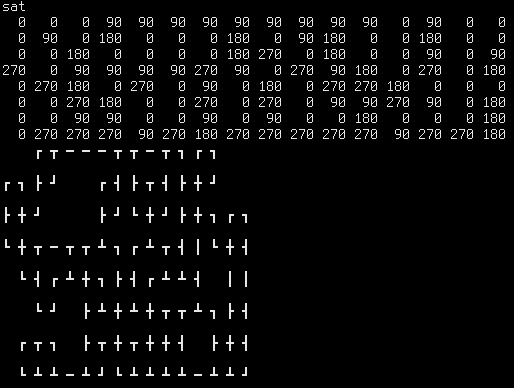
\includegraphics[scale=0.75]{\CURPATH/solver/solver.png}
\caption{Вывод скрипта солвера}
\end{figure}

Это работает $\approx 4$ секунды на моем старом и медленном Intel Atom N455 1.66GHz.
Быстро ли это? Не знаю, но снова вот что действительно круто, это то что мы понятия не имеем о какой-то математической
теории за всем этим, мы просто объявили ячейки, (полу-)стыки и определили отношения между ними.

Теперь следующий вопрос это, сколько здесь возможных решений?
Используя раннее описанный метод (\ref{SMTEnumerate}), я немного изменил скрипт солвера
\footnote{\url{.../solver/solve_pipe_puzzle2.py}} и солвер
сказал что возможно два решения.

Сравним их используя gvimdiff:

\begin{figure}[H]
\centering
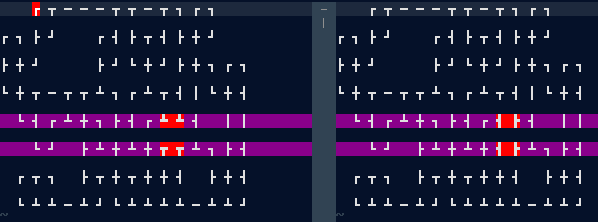
\includegraphics[scale=0.75]{\CURPATH/solver/diff.png}
\caption{Вывод gvimdiff (извините за мой красный курсор в левой части в левом верхнем углу)}
\end{figure}

4 ячейки в середине могут быть ориентированы по-разному.
Видимо, другие головоломки могут также выдавать разные результаты.

P.S.
\textit{Полу-стык} определен как булевый тип.
Но на самом деле, первая версия солвера была написана используя целочисленный тип для полу-стыков,
и 0 использовалось для False и 1 для True.
Я так сделал, потому что хотел более компактный исходный код, без использования длинных слов как ``False'' и ``True''.
И это работало, но медленнее. Вероятно, Z3 работает с булевыми типами быстрее? Лучше?
Так или иначе, я пишу это чтобы отметить, что, если нужно, целочисленный тип можно использовать вместо булевого.


\section{Развлекательная математика и головоломки}

\input{puzzles/sudoku/main_RU}
\input{puzzles/zebra/main_RU}
\input{puzzles/pipe/main_RU}
\input{puzzles/rubik2/failed_SMT/main_RU}
\input{puzzles/rubik2/SAT/main_RU}
\input{puzzles/rubik3/one_face_SMT/main_RU}
%\input{puzzles/numberlink/main_RU}
%\input{puzzles/two_parks_RU}
\input{puzzles/alphametics/main_RU}
%\input{puzzles/2015_AIME_II_Problems_12_RU}
%\input{puzzles/fred/main_RU}
%\input{puzzles/MC/main_RU}
%\input{puzzles/coin_flip/main_RU}
%\input{puzzles/Mock_AIME_2_2006-2007_Problem_8_RU}
%\input{puzzles/2012_AIME_I_Problems_1_RU}
%\input{puzzles/keypad_RU}


\section{Развлекательная математика и головоломки}

\input{puzzles/sudoku/main_RU}
\input{puzzles/zebra/main_RU}
\input{puzzles/pipe/main_RU}
\input{puzzles/rubik2/failed_SMT/main_RU}
\input{puzzles/rubik2/SAT/main_RU}
\input{puzzles/rubik3/one_face_SMT/main_RU}
%\input{puzzles/numberlink/main_RU}
%\input{puzzles/two_parks_RU}
\input{puzzles/alphametics/main_RU}
%\input{puzzles/2015_AIME_II_Problems_12_RU}
%\input{puzzles/fred/main_RU}
%\input{puzzles/MC/main_RU}
%\input{puzzles/coin_flip/main_RU}
%\input{puzzles/Mock_AIME_2_2006-2007_Problem_8_RU}
%\input{puzzles/2012_AIME_I_Problems_1_RU}
%\input{puzzles/keypad_RU}


\section{Развлекательная математика и головоломки}

\input{puzzles/sudoku/main_RU}
\input{puzzles/zebra/main_RU}
\input{puzzles/pipe/main_RU}
\input{puzzles/rubik2/failed_SMT/main_RU}
\input{puzzles/rubik2/SAT/main_RU}
\input{puzzles/rubik3/one_face_SMT/main_RU}
%\input{puzzles/numberlink/main_RU}
%\input{puzzles/two_parks_RU}
\input{puzzles/alphametics/main_RU}
%\input{puzzles/2015_AIME_II_Problems_12_RU}
%\input{puzzles/fred/main_RU}
%\input{puzzles/MC/main_RU}
%\input{puzzles/coin_flip/main_RU}
%\input{puzzles/Mock_AIME_2_2006-2007_Problem_8_RU}
%\input{puzzles/2012_AIME_I_Problems_1_RU}
%\input{puzzles/keypad_RU}


%\section{Развлекательная математика и головоломки}

\input{puzzles/sudoku/main_RU}
\input{puzzles/zebra/main_RU}
\input{puzzles/pipe/main_RU}
\input{puzzles/rubik2/failed_SMT/main_RU}
\input{puzzles/rubik2/SAT/main_RU}
\input{puzzles/rubik3/one_face_SMT/main_RU}
%\input{puzzles/numberlink/main_RU}
%\input{puzzles/two_parks_RU}
\input{puzzles/alphametics/main_RU}
%\input{puzzles/2015_AIME_II_Problems_12_RU}
%\input{puzzles/fred/main_RU}
%\input{puzzles/MC/main_RU}
%\input{puzzles/coin_flip/main_RU}
%\input{puzzles/Mock_AIME_2_2006-2007_Problem_8_RU}
%\input{puzzles/2012_AIME_I_Problems_1_RU}
%\input{puzzles/keypad_RU}


%\input{puzzles/two_parks_RU}
\subsection{Альфаметика}

Согласно Дональду Кнуту, термин ``Альфаметика'' был придуман Дж. Эйч. Аш. Хантером.
Это головоломка: какие десятичные цифры в пределах 0..9 нужно присвоить каждой букве, чтобы это уравнение было справедливо?

\begin{lstlisting}
  SEND
+ MORE
 -----
 MONEY
\end{lstlisting}

Для Z3 это легко:

\lstinputlisting{puzzles/alphametics/alpha.py}

Вывод:

\begin{lstlisting}
sat
[E, = 5,
 S, = 9,
 M, = 1,
 N, = 6,
 D, = 7,
 R, = 8,
 O, = 0,
 Y = 2]
\end{lstlisting}

Вот еще одна, из \ac{TAOCP} том IV (\url{http://www-cs-faculty.stanford.edu/~uno/fasc2b.ps.gz}):

\lstinputlisting{puzzles/alphametics/alpha2.py}

\begin{lstlisting}
sat
[L, = 6,
 S, = 7,
 N, = 2,
 T, = 1,
 I, = 5,
 V = 3,
 A, = 8,
 R, = 9,
 O, = 4,
 TRIO = 1954,
 SONATA, = 742818,
 VIOLA, = 35468,
 VIOLIN, = 354652]
\end{lstlisting}

% TODO URL
Эту головоломку я нашел в примерах pySMT:

\lstinputlisting{puzzles/alphametics/alpha3.py}

\begin{lstlisting}
sat
[D = 5, R = 4, O = 3, E = 8, L = 6, W = 7, H = 2]
\end{lstlisting}

%%% 

Это упражнение Q209 из
[Companion to the Papers of Donald Knuth]\footnote{\url{http://www-cs-faculty.stanford.edu/~knuth/cp.html}}.

\begin{lstlisting}
 KNIFE
  FORK
 SPOON
  SOUP
------
SUPPER
\end{lstlisting}

В целях упрощения, я добавил ф-цию (list\_to\_expr()):

\lstinputlisting{puzzles/alphametics/alpha4.py}

\begin{lstlisting}
sat
[K = 7,
 N = 4,
 R = 9,
 I = 1,
 E = 6,
 S = 0,
 O = 3,
 F = 5,
 U = 8,
 P = 2,
 SUPPER = 82269,
 SOUP = 382,
 SPOON = 2334,
 FORK = 5397,
 KNIFE = 74156]
\end{lstlisting}

S это 0, так что значение SUPPER начинается с (убранного) нуля. Скажем так, нам это не нравится.
Добавим это, чтобы это исправить:

\begin{lstlisting}
s.add(S!=0)
\end{lstlisting}

\begin{lstlisting}
sat
[K = 8,
 N = 4,
 R = 3,
 I = 7,
 E = 6,
 S = 1,
 O = 9,
 F = 2,
 U = 0,
 P = 5,
 SUPPER = 105563,
 SOUP = 1905,
 SPOON = 15994,
 FORK = 2938,
 KNIFE = 84726]
\end{lstlisting}

\paragraph{Создание своей собственной головоломки}

Вот проблема: есть только 10 букв, но как их выбрать из числа слов?
Мы можем использовать Z3 для этого:

\lstinputlisting{puzzles/alphametics/gen.py}

Это первая сгенерированная головоломка:

\begin{lstlisting}
sat
EGGS
JELLY
LUNCH
C 5
E 6
G 3
H 7
J 0
L 1
N 4
S 8
U 2
Y 9
\end{lstlisting}

Что если мы хотим, чтобы слово ``CAKE'' присутствовало в числе ``слагаемых''?

Добавим это:

\begin{lstlisting}
s.add(word_used[words.index('CAKE')])
\end{lstlisting}

\begin{lstlisting}
sat
CAKE
TEA
LUNCH
A 8
C 3
E 1
H 9
J 6
K 2
L 0
N 5
T 7
U 4
\end{lstlisting}

Добавим это:

\begin{lstlisting}
s.add(word_used[words.index('EGGS')])
\end{lstlisting}

Теперь оно может найти пару к EGGS:

\begin{lstlisting}
sat
EGGS
HONEY
LUNCH
C 6
E 7
G 9
H 4
L 5
N 8
O 2
S 3
U 0
Y 1
\end{lstlisting}

\paragraph{Файлы}

\url{https://github.com/DennisYurichev/...}




%\input{puzzles/2015_AIME_II_Problems_12_RU}
%\section{Развлекательная математика и головоломки}

\input{puzzles/sudoku/main_RU}
\input{puzzles/zebra/main_RU}
\input{puzzles/pipe/main_RU}
\input{puzzles/rubik2/failed_SMT/main_RU}
\input{puzzles/rubik2/SAT/main_RU}
\input{puzzles/rubik3/one_face_SMT/main_RU}
%\input{puzzles/numberlink/main_RU}
%\input{puzzles/two_parks_RU}
\input{puzzles/alphametics/main_RU}
%\input{puzzles/2015_AIME_II_Problems_12_RU}
%\input{puzzles/fred/main_RU}
%\input{puzzles/MC/main_RU}
%\input{puzzles/coin_flip/main_RU}
%\input{puzzles/Mock_AIME_2_2006-2007_Problem_8_RU}
%\input{puzzles/2012_AIME_I_Problems_1_RU}
%\input{puzzles/keypad_RU}


%\section{Развлекательная математика и головоломки}

\input{puzzles/sudoku/main_RU}
\input{puzzles/zebra/main_RU}
\input{puzzles/pipe/main_RU}
\input{puzzles/rubik2/failed_SMT/main_RU}
\input{puzzles/rubik2/SAT/main_RU}
\input{puzzles/rubik3/one_face_SMT/main_RU}
%\input{puzzles/numberlink/main_RU}
%\input{puzzles/two_parks_RU}
\input{puzzles/alphametics/main_RU}
%\input{puzzles/2015_AIME_II_Problems_12_RU}
%\input{puzzles/fred/main_RU}
%\input{puzzles/MC/main_RU}
%\input{puzzles/coin_flip/main_RU}
%\input{puzzles/Mock_AIME_2_2006-2007_Problem_8_RU}
%\input{puzzles/2012_AIME_I_Problems_1_RU}
%\input{puzzles/keypad_RU}


%\section{Развлекательная математика и головоломки}

\input{puzzles/sudoku/main_RU}
\input{puzzles/zebra/main_RU}
\input{puzzles/pipe/main_RU}
\input{puzzles/rubik2/failed_SMT/main_RU}
\input{puzzles/rubik2/SAT/main_RU}
\input{puzzles/rubik3/one_face_SMT/main_RU}
%\input{puzzles/numberlink/main_RU}
%\input{puzzles/two_parks_RU}
\input{puzzles/alphametics/main_RU}
%\input{puzzles/2015_AIME_II_Problems_12_RU}
%\input{puzzles/fred/main_RU}
%\input{puzzles/MC/main_RU}
%\input{puzzles/coin_flip/main_RU}
%\input{puzzles/Mock_AIME_2_2006-2007_Problem_8_RU}
%\input{puzzles/2012_AIME_I_Problems_1_RU}
%\input{puzzles/keypad_RU}


%\input{puzzles/Mock_AIME_2_2006-2007_Problem_8_RU}
%\input{puzzles/2012_AIME_I_Problems_1_RU}
%\input{puzzles/keypad_RU}


\section{Развлекательная математика и головоломки}

\subsection{Судоку}

Головоломка Судоку это решетка 9*9, некоторые ячейки заполнены значениями, некоторые пустые:

% copypasted from http://www.texample.net/tikz/examples/sudoku/
\newcounter{row}
\newcounter{col}

\newcommand\setrow[9]{
  \setcounter{col}{1}
  \foreach \n in {#1, #2, #3, #4, #5, #6, #7, #8, #9} {
    \edef\x{\value{col} - 0.5}
    \edef\y{9.5 - \value{row}}
    \node[anchor=center] at (\x, \y) {\n};
    \stepcounter{col}
  }
  \stepcounter{row}
}

\begin{center}
\begin{tikzpicture}[scale=.7]
  \begin{scope}
    \draw (0, 0) grid (9, 9);
    \draw[very thick, scale=3] (0, 0) grid (3, 3);

    \setcounter{row}{1}
    \setrow { }{ }{5}  {3}{ }{ }  { }{ }{ }
    \setrow {8}{ }{ }  { }{ }{ }  { }{2}{ }
    \setrow { }{7}{ }  { }{1}{ }  {5}{ }{ }

    \setrow {4}{ }{ }  { }{ }{5}  {3}{ }{ }
    \setrow { }{1}{ }  { }{7}{ }  { }{ }{6}
    \setrow { }{ }{3}  {2}{ }{ }  { }{8}{ }

    \setrow { }{6}{ }  {5}{ }{ }  { }{ }{9}
    \setrow { }{ }{4}  { }{ }{ }  { }{3}{ }
    \setrow { }{ }{ }  { }{ }{9}  {7}{ }{ }

    \node[anchor=center] at (4.5, -0.5) {Нерешенная Судоку};
  \end{scope}
\end{tikzpicture}
\end{center}

Числа в каждом ряду должны быть уникальными, т.е., каждый ряд должен содержать 9 чисел в пределах 1..9 без повторений.
Та же история и для каждого столбца и каждого квадрата 3*3.

Головоломка представляет собой хороший кандидат, на котором можно попробовать \ac{SMT}-солвер, потому что это,
в общем-то, просто нерешенная система уравнений.

\input{puzzles/sudoku/1/main_RU}
%\input{puzzles/sudoku/GT/main_RU}
%\input{puzzles/sudoku/killer/main_RU}
\input{puzzles/sudoku/KLEE/main_RU}
\input{puzzles/sudoku/SAT/main_RU}


\subsection{Головоломка зебры (\ac{AKA} Загадка Эйнштейна)}

\input{puzzles/zebra/SMT/main_RU}
\input{puzzles/zebra/KLEE/main_RU}
\input{puzzles/zebra/SAT/main_RU}


\subsection{Решение головоломки ``трубы'' используя Z3 SMT-солвер}

\renewcommand{\CURPATH}{puzzles/pipe}

Головоломка ``трубы'' это популярная головоломка (просто погуглите ``pipe puzzle'' и посмотрите на картинки).

Вот как выглядит головоломка в разобранном виде:

\begin{figure}[H]
\label{fig:pipe_shuffled}
\centering
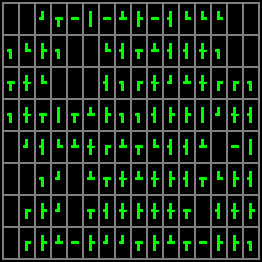
\includegraphics[scale=0.75]{\CURPATH/shuffled.png}
\caption{Разобранная головоломка}
\end{figure}

\dots и собранная:

\begin{figure}[H]
\label{fig:pipe_solved}
\centering
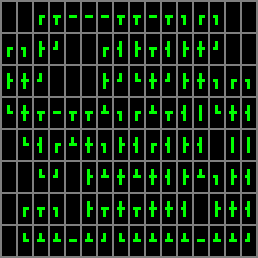
\includegraphics[scale=0.75]{\CURPATH/solved.png}
\caption{Собранная головоломка}
\end{figure}

Попробуем найти способ собрать её.

\subsubsection{Создание}

В начале, нужно её создать.
Вот простая идея.
Возьем массив ячеек 8*16.
Каждая ячейка может содержать какой-то тип блока.
Между ячейками есть стыки:

\input{\CURPATH/pipe_gen.tex}

Синие линии это горизонтальные стыки, красные линии это вертикальные стыки.
Мы просто случайно выставляем каждый стык в 0/false (отсутствует) или 1/true (присутствует).

После этого, теперь легко найти тип каждой ячейки.
А это:

\newcommand{\HeaderColor}{\cellcolor{blue!25}}
\begin{center}
\begin{longtable}{ | l | l | l | l | }
\hline
\HeaderColor стыки & \HeaderColor наше внутреннее название & \HeaderColor угол & \HeaderColor символ \\
\hline
0	&type 0		&	0$^{\circ}$	& (пробел)	\\
2	&type 2a	&	0$^{\circ}$	& \pmboxdrawuni{2503} \\ % ┃
2	&type 2a	&	90$^{\circ}$	& \pmboxdrawuni{2501} \\ % ━
2	&type 2b	&	0$^{\circ}$	& \pmboxdrawuni{250F} \\ % ┏
2	&type 2b	&	90$^{\circ}$	& \pmboxdrawuni{2513} \\ % ┓
2	&type 2b	&	180$^{\circ}$	& \pmboxdrawuni{251B} \\ % ┛
2	&type 2b	&	270$^{\circ}$	& \pmboxdrawuni{2517} \\ % ┗
3	&type 3		&	0$^{\circ}$	& \pmboxdrawuni{2523} \\ % ┣
3 	&type 3		&	90$^{\circ}$	& \pmboxdrawuni{2533} \\ % ┳
3	&type 3		&	180$^{\circ}$	& \pmboxdrawuni{252B} \\ % ┫
3	&type 3		&	270$^{\circ}$	& \pmboxdrawuni{253B} \\ % ┻
4	&type 4		&	0$^{\circ}$	& \pmboxdrawuni{254B} \\ % ╋
\hline
\end{longtable}
\end{center}

\textit{Висящие} стыки могут присутствовать на первой стадии (т.е., ячейки только с одним стыком), но они удалются
рекурсивно, и эти ячейки преобразуются в пустые ячейки.
Так что, в самом конце, все ячейки имеют минимум 2 стыка, и вся эта сантехническая система не имеет связей с внешним миром ---
я надеюсь, из-за этого станет немного проще.

Исходник генератора на Си здесь: \url{.../pipe/generator}.
Все вертикальные стыки хранятся в глобальном массиве \textit{hjoints[]} и вертикальные в \textit{vjoints[]}.

Программа на Си генерирует ANSI-раскрашенный вывод, как это было показано выше
(\ref{fig:pipe_shuffled}, \ref{fig:pipe_solved}) плюс массив типов для каждой ячейки, но без информации об углах:

\begin{lstlisting}[label=init_cells]
[
["0", "0", "2b", "3", "2a", "2a", "2a", "3", "3", "2a", "3", "2b", "2b", "2b", "0", "0"],
["2b", "2b", "3", "2b", "0", "0", "2b", "3", "3", "3", "3", "3", "4", "2b", "0", "0"],
["3", "4", "2b", "0", "0", "0", "3", "2b", "2b", "4", "2b", "3", "4", "2b", "2b", "2b"],
["2b", "4", "3", "2a", "3", "3", "3", "2b", "2b", "3", "3", "3", "2a", "2b", "4", "3"],
["0", "2b", "3", "2b", "3", "4", "2b", "3", "3", "2b", "3", "3", "3", "0", "2a", "2a"],
["0", "0", "2b", "2b", "0", "3", "3", "4", "3", "4", "3", "3", "3", "2b", "3", "3"],
["0", "2b", "3", "2b", "0", "3", "3", "4", "3", "4", "4", "3", "0", "3", "4", "3"],
["0", "2b", "3", "3", "2a", "3", "2b", "2b", "3", "3", "3", "3", "2a", "3", "3", "2b"],
]
\end{lstlisting}

\subsubsection{Решение}

Прежде всего, мы будем работать с массивом ячеек 8*16, где каждый элемент имеет 4 бита:
``T'' (top/верх),
``B'' (bottom/низ),
``L'' (left/лево),
``R'' (right/право).
Каждый бит представляет собой половину стыка.

\input{\CURPATH/pipe_solve.tex}

Теперь определяем массив для каждого из четырех полустыков + информация об угле:

\begin{lstlisting}
HEIGHT=8
WIDTH=16

# if T/B/R/L is Bool instead of Int, Z3 solver will work faster
T=[[Bool('cell_%d_%d_top' % (r, c)) for c in range(WIDTH)] for r in range(HEIGHT)]
B=[[Bool('cell_%d_%d_bottom' % (r, c)) for c in range(WIDTH)] for r in range(HEIGHT)]
R=[[Bool('cell_%d_%d_right' % (r, c)) for c in range(WIDTH)] for r in range(HEIGHT)]
L=[[Bool('cell_%d_%d_left' % (r, c)) for c in range(WIDTH)] for r in range(HEIGHT)]
A=[[Int('cell_%d_%d_angle' % (r, c)) for c in range(WIDTH)] for r in range(HEIGHT)]
\end{lstlisting}

Мы знаем, что если каждый из полустыков присутствует, ответный полустык также должен присутствовать, и наоборот. 
Определяем всё это используя эти констрайнты:

\begin{lstlisting}
# shorthand variables for True and False:
t=True
f=False

# "top" of each cell must be equal to "bottom" of the cell above
# "bottom" of each cell must be equal to "top" of the cell below
# "left" of each cell must be equal to "right" of the cell at left
# "right" of each cell must be equal to "left" of the cell at right
for r in range(HEIGHT):
    for c in range(WIDTH):
        if r!=0:
            s.add(T[r][c]==B[r-1][c])
        if r!=HEIGHT-1:
            s.add(B[r][c]==T[r+1][c])
        if c!=0:
            s.add(L[r][c]==R[r][c-1])
        if c!=WIDTH-1:
            s.add(R[r][c]==L[r][c+1])

# "left" of each cell of first column shouldn't have any connection
# so is "right" of each cell of the last column
for r in range(HEIGHT):
    s.add(L[r][0]==f)
    s.add(R[r][WIDTH-1]==f)

# "top" of each cell of the first row shouldn't have any connection
# so is "bottom" of each cell of the last row
for c in range(WIDTH):
    s.add(T[0][c]==f)
    s.add(B[HEIGHT-1][c]==f)
\end{lstlisting}

Теперь перебираем все ячейки в изначальном массиве (\ref{init_cells}).
Первые две ячейки здесь пустые. И третья имеет тип ``2b''.
Это ``\pmboxdrawuni{250F}'' % ┏
и его можно ориентировать четырьмя разными способами.
И если её угол это 0$^{\circ}$, верхний и правый полустыки присутствуют, остальные отсутствуют.
Если он имеет угол 90$^{\circ}$, он выглядит как 
``\pmboxdrawuni{2513}'', % ┓
и верхник и левый полустыки присутствуют, остальные отсутствуют.

На обычном русском языке: ``если ячейка этого типа имеет угол 0$^{\circ}$, вот эти полустыки должны присутствовать \textbf{ИЛИ}
если она имеет угол 90$^{\circ}$, эти полустыки должны присутствовать, \textbf{ИЛИ}, итд, итд.''

Точно также, мы определяем эти правила для всех типов и всех возможных углов:

\begin{lstlisting}
for r in range(HEIGHT):
    for c in range(WIDTH):
        ty=cells_type[r][c]

        if ty=="0":
            s.add(A[r][c]==f)
            s.add(T[r][c]==f, B[r][c]==f, L[r][c]==f, R[r][c]==f)

        if ty=="2a":
            s.add(Or(And(A[r][c]==0, L[r][c]==f, R[r][c]==f, T[r][c]==t, B[r][c]==t),   # §\pmboxdrawuni{2503}§
                    And(A[r][c]==90, L[r][c]==t, R[r][c]==t, T[r][c]==f, B[r][c]==f)))  # §\pmboxdrawuni{2501}§

        if ty=="2b":
            s.add(Or(And(A[r][c]==0, L[r][c]==f, R[r][c]==t, T[r][c]==f, B[r][c]==t),   # §\pmboxdrawuni{250F}§
                    And(A[r][c]==90, L[r][c]==t, R[r][c]==f, T[r][c]==f, B[r][c]==t),   # §\pmboxdrawuni{2513}§
                    And(A[r][c]==180, L[r][c]==t, R[r][c]==f, T[r][c]==t, B[r][c]==f),  # §\pmboxdrawuni{251B}§
                    And(A[r][c]==270, L[r][c]==f, R[r][c]==t, T[r][c]==t, B[r][c]==f))) # §\pmboxdrawuni{2517}§
	
        if ty=="3":
            s.add(Or(And(A[r][c]==0, L[r][c]==f, R[r][c]==t, T[r][c]==t, B[r][c]==t),   # §\pmboxdrawuni{2523}§
                    And(A[r][c]==90, L[r][c]==t, R[r][c]==t, T[r][c]==f, B[r][c]==t),   # §\pmboxdrawuni{2533}§
                    And(A[r][c]==180, L[r][c]==t, R[r][c]==f, T[r][c]==t, B[r][c]==t),  # §\pmboxdrawuni{252B}§
                    And(A[r][c]==270, L[r][c]==t, R[r][c]==t, T[r][c]==t, B[r][c]==f))) # §\pmboxdrawuni{253B}§

        if ty=="4":
            s.add(A[r][c]==0)
            s.add(T[r][c]==t, B[r][c]==t, L[r][c]==t, R[r][c]==t) # §\pmboxdrawuni{254B}§
\end{lstlisting}

Полный исходник здесь: \url{.../solver/solve_pipe_puzzle1.py}.

Получается такой результат (выводит угол для каждой ячейки и (псевдо)графическое представление):

\begin{figure}[H]
\centering
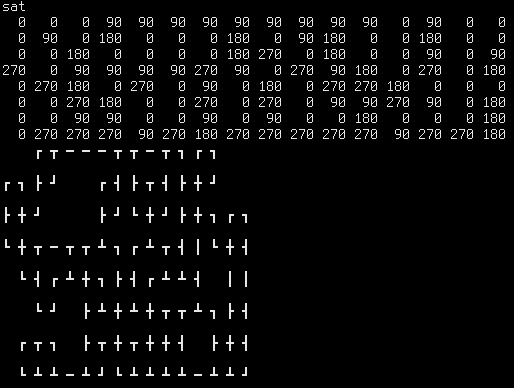
\includegraphics[scale=0.75]{\CURPATH/solver/solver.png}
\caption{Вывод скрипта солвера}
\end{figure}

Это работает $\approx 4$ секунды на моем старом и медленном Intel Atom N455 1.66GHz.
Быстро ли это? Не знаю, но снова вот что действительно круто, это то что мы понятия не имеем о какой-то математической
теории за всем этим, мы просто объявили ячейки, (полу-)стыки и определили отношения между ними.

Теперь следующий вопрос это, сколько здесь возможных решений?
Используя раннее описанный метод (\ref{SMTEnumerate}), я немного изменил скрипт солвера
\footnote{\url{.../solver/solve_pipe_puzzle2.py}} и солвер
сказал что возможно два решения.

Сравним их используя gvimdiff:

\begin{figure}[H]
\centering
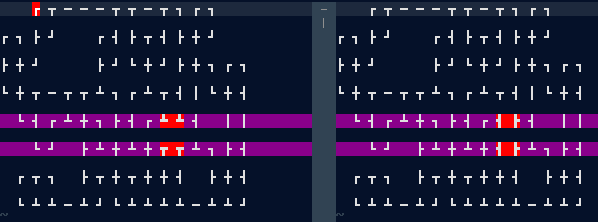
\includegraphics[scale=0.75]{\CURPATH/solver/diff.png}
\caption{Вывод gvimdiff (извините за мой красный курсор в левой части в левом верхнем углу)}
\end{figure}

4 ячейки в середине могут быть ориентированы по-разному.
Видимо, другие головоломки могут также выдавать разные результаты.

P.S.
\textit{Полу-стык} определен как булевый тип.
Но на самом деле, первая версия солвера была написана используя целочисленный тип для полу-стыков,
и 0 использовалось для False и 1 для True.
Я так сделал, потому что хотел более компактный исходный код, без использования длинных слов как ``False'' и ``True''.
И это работало, но медленнее. Вероятно, Z3 работает с булевыми типами быстрее? Лучше?
Так или иначе, я пишу это чтобы отметить, что, если нужно, целочисленный тип можно использовать вместо булевого.


\section{Развлекательная математика и головоломки}

\input{puzzles/sudoku/main_RU}
\input{puzzles/zebra/main_RU}
\input{puzzles/pipe/main_RU}
\input{puzzles/rubik2/failed_SMT/main_RU}
\input{puzzles/rubik2/SAT/main_RU}
\input{puzzles/rubik3/one_face_SMT/main_RU}
%\input{puzzles/numberlink/main_RU}
%\input{puzzles/two_parks_RU}
\input{puzzles/alphametics/main_RU}
%\input{puzzles/2015_AIME_II_Problems_12_RU}
%\input{puzzles/fred/main_RU}
%\input{puzzles/MC/main_RU}
%\input{puzzles/coin_flip/main_RU}
%\input{puzzles/Mock_AIME_2_2006-2007_Problem_8_RU}
%\input{puzzles/2012_AIME_I_Problems_1_RU}
%\input{puzzles/keypad_RU}


\section{Развлекательная математика и головоломки}

\input{puzzles/sudoku/main_RU}
\input{puzzles/zebra/main_RU}
\input{puzzles/pipe/main_RU}
\input{puzzles/rubik2/failed_SMT/main_RU}
\input{puzzles/rubik2/SAT/main_RU}
\input{puzzles/rubik3/one_face_SMT/main_RU}
%\input{puzzles/numberlink/main_RU}
%\input{puzzles/two_parks_RU}
\input{puzzles/alphametics/main_RU}
%\input{puzzles/2015_AIME_II_Problems_12_RU}
%\input{puzzles/fred/main_RU}
%\input{puzzles/MC/main_RU}
%\input{puzzles/coin_flip/main_RU}
%\input{puzzles/Mock_AIME_2_2006-2007_Problem_8_RU}
%\input{puzzles/2012_AIME_I_Problems_1_RU}
%\input{puzzles/keypad_RU}


\section{Развлекательная математика и головоломки}

\input{puzzles/sudoku/main_RU}
\input{puzzles/zebra/main_RU}
\input{puzzles/pipe/main_RU}
\input{puzzles/rubik2/failed_SMT/main_RU}
\input{puzzles/rubik2/SAT/main_RU}
\input{puzzles/rubik3/one_face_SMT/main_RU}
%\input{puzzles/numberlink/main_RU}
%\input{puzzles/two_parks_RU}
\input{puzzles/alphametics/main_RU}
%\input{puzzles/2015_AIME_II_Problems_12_RU}
%\input{puzzles/fred/main_RU}
%\input{puzzles/MC/main_RU}
%\input{puzzles/coin_flip/main_RU}
%\input{puzzles/Mock_AIME_2_2006-2007_Problem_8_RU}
%\input{puzzles/2012_AIME_I_Problems_1_RU}
%\input{puzzles/keypad_RU}


%\section{Развлекательная математика и головоломки}

\input{puzzles/sudoku/main_RU}
\input{puzzles/zebra/main_RU}
\input{puzzles/pipe/main_RU}
\input{puzzles/rubik2/failed_SMT/main_RU}
\input{puzzles/rubik2/SAT/main_RU}
\input{puzzles/rubik3/one_face_SMT/main_RU}
%\input{puzzles/numberlink/main_RU}
%\input{puzzles/two_parks_RU}
\input{puzzles/alphametics/main_RU}
%\input{puzzles/2015_AIME_II_Problems_12_RU}
%\input{puzzles/fred/main_RU}
%\input{puzzles/MC/main_RU}
%\input{puzzles/coin_flip/main_RU}
%\input{puzzles/Mock_AIME_2_2006-2007_Problem_8_RU}
%\input{puzzles/2012_AIME_I_Problems_1_RU}
%\input{puzzles/keypad_RU}


%\input{puzzles/two_parks_RU}
\subsection{Альфаметика}

Согласно Дональду Кнуту, термин ``Альфаметика'' был придуман Дж. Эйч. Аш. Хантером.
Это головоломка: какие десятичные цифры в пределах 0..9 нужно присвоить каждой букве, чтобы это уравнение было справедливо?

\begin{lstlisting}
  SEND
+ MORE
 -----
 MONEY
\end{lstlisting}

Для Z3 это легко:

\lstinputlisting{puzzles/alphametics/alpha.py}

Вывод:

\begin{lstlisting}
sat
[E, = 5,
 S, = 9,
 M, = 1,
 N, = 6,
 D, = 7,
 R, = 8,
 O, = 0,
 Y = 2]
\end{lstlisting}

Вот еще одна, из \ac{TAOCP} том IV (\url{http://www-cs-faculty.stanford.edu/~uno/fasc2b.ps.gz}):

\lstinputlisting{puzzles/alphametics/alpha2.py}

\begin{lstlisting}
sat
[L, = 6,
 S, = 7,
 N, = 2,
 T, = 1,
 I, = 5,
 V = 3,
 A, = 8,
 R, = 9,
 O, = 4,
 TRIO = 1954,
 SONATA, = 742818,
 VIOLA, = 35468,
 VIOLIN, = 354652]
\end{lstlisting}

% TODO URL
Эту головоломку я нашел в примерах pySMT:

\lstinputlisting{puzzles/alphametics/alpha3.py}

\begin{lstlisting}
sat
[D = 5, R = 4, O = 3, E = 8, L = 6, W = 7, H = 2]
\end{lstlisting}

%%% 

Это упражнение Q209 из
[Companion to the Papers of Donald Knuth]\footnote{\url{http://www-cs-faculty.stanford.edu/~knuth/cp.html}}.

\begin{lstlisting}
 KNIFE
  FORK
 SPOON
  SOUP
------
SUPPER
\end{lstlisting}

В целях упрощения, я добавил ф-цию (list\_to\_expr()):

\lstinputlisting{puzzles/alphametics/alpha4.py}

\begin{lstlisting}
sat
[K = 7,
 N = 4,
 R = 9,
 I = 1,
 E = 6,
 S = 0,
 O = 3,
 F = 5,
 U = 8,
 P = 2,
 SUPPER = 82269,
 SOUP = 382,
 SPOON = 2334,
 FORK = 5397,
 KNIFE = 74156]
\end{lstlisting}

S это 0, так что значение SUPPER начинается с (убранного) нуля. Скажем так, нам это не нравится.
Добавим это, чтобы это исправить:

\begin{lstlisting}
s.add(S!=0)
\end{lstlisting}

\begin{lstlisting}
sat
[K = 8,
 N = 4,
 R = 3,
 I = 7,
 E = 6,
 S = 1,
 O = 9,
 F = 2,
 U = 0,
 P = 5,
 SUPPER = 105563,
 SOUP = 1905,
 SPOON = 15994,
 FORK = 2938,
 KNIFE = 84726]
\end{lstlisting}

\paragraph{Создание своей собственной головоломки}

Вот проблема: есть только 10 букв, но как их выбрать из числа слов?
Мы можем использовать Z3 для этого:

\lstinputlisting{puzzles/alphametics/gen.py}

Это первая сгенерированная головоломка:

\begin{lstlisting}
sat
EGGS
JELLY
LUNCH
C 5
E 6
G 3
H 7
J 0
L 1
N 4
S 8
U 2
Y 9
\end{lstlisting}

Что если мы хотим, чтобы слово ``CAKE'' присутствовало в числе ``слагаемых''?

Добавим это:

\begin{lstlisting}
s.add(word_used[words.index('CAKE')])
\end{lstlisting}

\begin{lstlisting}
sat
CAKE
TEA
LUNCH
A 8
C 3
E 1
H 9
J 6
K 2
L 0
N 5
T 7
U 4
\end{lstlisting}

Добавим это:

\begin{lstlisting}
s.add(word_used[words.index('EGGS')])
\end{lstlisting}

Теперь оно может найти пару к EGGS:

\begin{lstlisting}
sat
EGGS
HONEY
LUNCH
C 6
E 7
G 9
H 4
L 5
N 8
O 2
S 3
U 0
Y 1
\end{lstlisting}

\paragraph{Файлы}

\url{https://github.com/DennisYurichev/...}




%\input{puzzles/2015_AIME_II_Problems_12_RU}
%\section{Развлекательная математика и головоломки}

\input{puzzles/sudoku/main_RU}
\input{puzzles/zebra/main_RU}
\input{puzzles/pipe/main_RU}
\input{puzzles/rubik2/failed_SMT/main_RU}
\input{puzzles/rubik2/SAT/main_RU}
\input{puzzles/rubik3/one_face_SMT/main_RU}
%\input{puzzles/numberlink/main_RU}
%\input{puzzles/two_parks_RU}
\input{puzzles/alphametics/main_RU}
%\input{puzzles/2015_AIME_II_Problems_12_RU}
%\input{puzzles/fred/main_RU}
%\input{puzzles/MC/main_RU}
%\input{puzzles/coin_flip/main_RU}
%\input{puzzles/Mock_AIME_2_2006-2007_Problem_8_RU}
%\input{puzzles/2012_AIME_I_Problems_1_RU}
%\input{puzzles/keypad_RU}


%\section{Развлекательная математика и головоломки}

\input{puzzles/sudoku/main_RU}
\input{puzzles/zebra/main_RU}
\input{puzzles/pipe/main_RU}
\input{puzzles/rubik2/failed_SMT/main_RU}
\input{puzzles/rubik2/SAT/main_RU}
\input{puzzles/rubik3/one_face_SMT/main_RU}
%\input{puzzles/numberlink/main_RU}
%\input{puzzles/two_parks_RU}
\input{puzzles/alphametics/main_RU}
%\input{puzzles/2015_AIME_II_Problems_12_RU}
%\input{puzzles/fred/main_RU}
%\input{puzzles/MC/main_RU}
%\input{puzzles/coin_flip/main_RU}
%\input{puzzles/Mock_AIME_2_2006-2007_Problem_8_RU}
%\input{puzzles/2012_AIME_I_Problems_1_RU}
%\input{puzzles/keypad_RU}


%\section{Развлекательная математика и головоломки}

\input{puzzles/sudoku/main_RU}
\input{puzzles/zebra/main_RU}
\input{puzzles/pipe/main_RU}
\input{puzzles/rubik2/failed_SMT/main_RU}
\input{puzzles/rubik2/SAT/main_RU}
\input{puzzles/rubik3/one_face_SMT/main_RU}
%\input{puzzles/numberlink/main_RU}
%\input{puzzles/two_parks_RU}
\input{puzzles/alphametics/main_RU}
%\input{puzzles/2015_AIME_II_Problems_12_RU}
%\input{puzzles/fred/main_RU}
%\input{puzzles/MC/main_RU}
%\input{puzzles/coin_flip/main_RU}
%\input{puzzles/Mock_AIME_2_2006-2007_Problem_8_RU}
%\input{puzzles/2012_AIME_I_Problems_1_RU}
%\input{puzzles/keypad_RU}


%\input{puzzles/Mock_AIME_2_2006-2007_Problem_8_RU}
%\input{puzzles/2012_AIME_I_Problems_1_RU}
%\input{puzzles/keypad_RU}


%\section{Развлекательная математика и головоломки}

\subsection{Судоку}

Головоломка Судоку это решетка 9*9, некоторые ячейки заполнены значениями, некоторые пустые:

% copypasted from http://www.texample.net/tikz/examples/sudoku/
\newcounter{row}
\newcounter{col}

\newcommand\setrow[9]{
  \setcounter{col}{1}
  \foreach \n in {#1, #2, #3, #4, #5, #6, #7, #8, #9} {
    \edef\x{\value{col} - 0.5}
    \edef\y{9.5 - \value{row}}
    \node[anchor=center] at (\x, \y) {\n};
    \stepcounter{col}
  }
  \stepcounter{row}
}

\begin{center}
\begin{tikzpicture}[scale=.7]
  \begin{scope}
    \draw (0, 0) grid (9, 9);
    \draw[very thick, scale=3] (0, 0) grid (3, 3);

    \setcounter{row}{1}
    \setrow { }{ }{5}  {3}{ }{ }  { }{ }{ }
    \setrow {8}{ }{ }  { }{ }{ }  { }{2}{ }
    \setrow { }{7}{ }  { }{1}{ }  {5}{ }{ }

    \setrow {4}{ }{ }  { }{ }{5}  {3}{ }{ }
    \setrow { }{1}{ }  { }{7}{ }  { }{ }{6}
    \setrow { }{ }{3}  {2}{ }{ }  { }{8}{ }

    \setrow { }{6}{ }  {5}{ }{ }  { }{ }{9}
    \setrow { }{ }{4}  { }{ }{ }  { }{3}{ }
    \setrow { }{ }{ }  { }{ }{9}  {7}{ }{ }

    \node[anchor=center] at (4.5, -0.5) {Нерешенная Судоку};
  \end{scope}
\end{tikzpicture}
\end{center}

Числа в каждом ряду должны быть уникальными, т.е., каждый ряд должен содержать 9 чисел в пределах 1..9 без повторений.
Та же история и для каждого столбца и каждого квадрата 3*3.

Головоломка представляет собой хороший кандидат, на котором можно попробовать \ac{SMT}-солвер, потому что это,
в общем-то, просто нерешенная система уравнений.

\input{puzzles/sudoku/1/main_RU}
%\input{puzzles/sudoku/GT/main_RU}
%\input{puzzles/sudoku/killer/main_RU}
\input{puzzles/sudoku/KLEE/main_RU}
\input{puzzles/sudoku/SAT/main_RU}


\subsection{Головоломка зебры (\ac{AKA} Загадка Эйнштейна)}

\input{puzzles/zebra/SMT/main_RU}
\input{puzzles/zebra/KLEE/main_RU}
\input{puzzles/zebra/SAT/main_RU}


\subsection{Решение головоломки ``трубы'' используя Z3 SMT-солвер}

\renewcommand{\CURPATH}{puzzles/pipe}

Головоломка ``трубы'' это популярная головоломка (просто погуглите ``pipe puzzle'' и посмотрите на картинки).

Вот как выглядит головоломка в разобранном виде:

\begin{figure}[H]
\label{fig:pipe_shuffled}
\centering
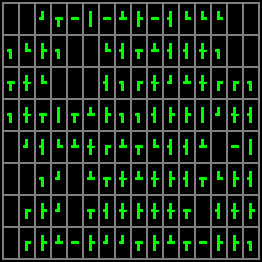
\includegraphics[scale=0.75]{\CURPATH/shuffled.png}
\caption{Разобранная головоломка}
\end{figure}

\dots и собранная:

\begin{figure}[H]
\label{fig:pipe_solved}
\centering
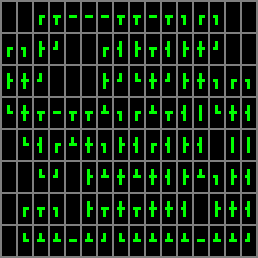
\includegraphics[scale=0.75]{\CURPATH/solved.png}
\caption{Собранная головоломка}
\end{figure}

Попробуем найти способ собрать её.

\subsubsection{Создание}

В начале, нужно её создать.
Вот простая идея.
Возьем массив ячеек 8*16.
Каждая ячейка может содержать какой-то тип блока.
Между ячейками есть стыки:

\input{\CURPATH/pipe_gen.tex}

Синие линии это горизонтальные стыки, красные линии это вертикальные стыки.
Мы просто случайно выставляем каждый стык в 0/false (отсутствует) или 1/true (присутствует).

После этого, теперь легко найти тип каждой ячейки.
А это:

\newcommand{\HeaderColor}{\cellcolor{blue!25}}
\begin{center}
\begin{longtable}{ | l | l | l | l | }
\hline
\HeaderColor стыки & \HeaderColor наше внутреннее название & \HeaderColor угол & \HeaderColor символ \\
\hline
0	&type 0		&	0$^{\circ}$	& (пробел)	\\
2	&type 2a	&	0$^{\circ}$	& \pmboxdrawuni{2503} \\ % ┃
2	&type 2a	&	90$^{\circ}$	& \pmboxdrawuni{2501} \\ % ━
2	&type 2b	&	0$^{\circ}$	& \pmboxdrawuni{250F} \\ % ┏
2	&type 2b	&	90$^{\circ}$	& \pmboxdrawuni{2513} \\ % ┓
2	&type 2b	&	180$^{\circ}$	& \pmboxdrawuni{251B} \\ % ┛
2	&type 2b	&	270$^{\circ}$	& \pmboxdrawuni{2517} \\ % ┗
3	&type 3		&	0$^{\circ}$	& \pmboxdrawuni{2523} \\ % ┣
3 	&type 3		&	90$^{\circ}$	& \pmboxdrawuni{2533} \\ % ┳
3	&type 3		&	180$^{\circ}$	& \pmboxdrawuni{252B} \\ % ┫
3	&type 3		&	270$^{\circ}$	& \pmboxdrawuni{253B} \\ % ┻
4	&type 4		&	0$^{\circ}$	& \pmboxdrawuni{254B} \\ % ╋
\hline
\end{longtable}
\end{center}

\textit{Висящие} стыки могут присутствовать на первой стадии (т.е., ячейки только с одним стыком), но они удалются
рекурсивно, и эти ячейки преобразуются в пустые ячейки.
Так что, в самом конце, все ячейки имеют минимум 2 стыка, и вся эта сантехническая система не имеет связей с внешним миром ---
я надеюсь, из-за этого станет немного проще.

Исходник генератора на Си здесь: \url{.../pipe/generator}.
Все вертикальные стыки хранятся в глобальном массиве \textit{hjoints[]} и вертикальные в \textit{vjoints[]}.

Программа на Си генерирует ANSI-раскрашенный вывод, как это было показано выше
(\ref{fig:pipe_shuffled}, \ref{fig:pipe_solved}) плюс массив типов для каждой ячейки, но без информации об углах:

\begin{lstlisting}[label=init_cells]
[
["0", "0", "2b", "3", "2a", "2a", "2a", "3", "3", "2a", "3", "2b", "2b", "2b", "0", "0"],
["2b", "2b", "3", "2b", "0", "0", "2b", "3", "3", "3", "3", "3", "4", "2b", "0", "0"],
["3", "4", "2b", "0", "0", "0", "3", "2b", "2b", "4", "2b", "3", "4", "2b", "2b", "2b"],
["2b", "4", "3", "2a", "3", "3", "3", "2b", "2b", "3", "3", "3", "2a", "2b", "4", "3"],
["0", "2b", "3", "2b", "3", "4", "2b", "3", "3", "2b", "3", "3", "3", "0", "2a", "2a"],
["0", "0", "2b", "2b", "0", "3", "3", "4", "3", "4", "3", "3", "3", "2b", "3", "3"],
["0", "2b", "3", "2b", "0", "3", "3", "4", "3", "4", "4", "3", "0", "3", "4", "3"],
["0", "2b", "3", "3", "2a", "3", "2b", "2b", "3", "3", "3", "3", "2a", "3", "3", "2b"],
]
\end{lstlisting}

\subsubsection{Решение}

Прежде всего, мы будем работать с массивом ячеек 8*16, где каждый элемент имеет 4 бита:
``T'' (top/верх),
``B'' (bottom/низ),
``L'' (left/лево),
``R'' (right/право).
Каждый бит представляет собой половину стыка.

\input{\CURPATH/pipe_solve.tex}

Теперь определяем массив для каждого из четырех полустыков + информация об угле:

\begin{lstlisting}
HEIGHT=8
WIDTH=16

# if T/B/R/L is Bool instead of Int, Z3 solver will work faster
T=[[Bool('cell_%d_%d_top' % (r, c)) for c in range(WIDTH)] for r in range(HEIGHT)]
B=[[Bool('cell_%d_%d_bottom' % (r, c)) for c in range(WIDTH)] for r in range(HEIGHT)]
R=[[Bool('cell_%d_%d_right' % (r, c)) for c in range(WIDTH)] for r in range(HEIGHT)]
L=[[Bool('cell_%d_%d_left' % (r, c)) for c in range(WIDTH)] for r in range(HEIGHT)]
A=[[Int('cell_%d_%d_angle' % (r, c)) for c in range(WIDTH)] for r in range(HEIGHT)]
\end{lstlisting}

Мы знаем, что если каждый из полустыков присутствует, ответный полустык также должен присутствовать, и наоборот. 
Определяем всё это используя эти констрайнты:

\begin{lstlisting}
# shorthand variables for True and False:
t=True
f=False

# "top" of each cell must be equal to "bottom" of the cell above
# "bottom" of each cell must be equal to "top" of the cell below
# "left" of each cell must be equal to "right" of the cell at left
# "right" of each cell must be equal to "left" of the cell at right
for r in range(HEIGHT):
    for c in range(WIDTH):
        if r!=0:
            s.add(T[r][c]==B[r-1][c])
        if r!=HEIGHT-1:
            s.add(B[r][c]==T[r+1][c])
        if c!=0:
            s.add(L[r][c]==R[r][c-1])
        if c!=WIDTH-1:
            s.add(R[r][c]==L[r][c+1])

# "left" of each cell of first column shouldn't have any connection
# so is "right" of each cell of the last column
for r in range(HEIGHT):
    s.add(L[r][0]==f)
    s.add(R[r][WIDTH-1]==f)

# "top" of each cell of the first row shouldn't have any connection
# so is "bottom" of each cell of the last row
for c in range(WIDTH):
    s.add(T[0][c]==f)
    s.add(B[HEIGHT-1][c]==f)
\end{lstlisting}

Теперь перебираем все ячейки в изначальном массиве (\ref{init_cells}).
Первые две ячейки здесь пустые. И третья имеет тип ``2b''.
Это ``\pmboxdrawuni{250F}'' % ┏
и его можно ориентировать четырьмя разными способами.
И если её угол это 0$^{\circ}$, верхний и правый полустыки присутствуют, остальные отсутствуют.
Если он имеет угол 90$^{\circ}$, он выглядит как 
``\pmboxdrawuni{2513}'', % ┓
и верхник и левый полустыки присутствуют, остальные отсутствуют.

На обычном русском языке: ``если ячейка этого типа имеет угол 0$^{\circ}$, вот эти полустыки должны присутствовать \textbf{ИЛИ}
если она имеет угол 90$^{\circ}$, эти полустыки должны присутствовать, \textbf{ИЛИ}, итд, итд.''

Точно также, мы определяем эти правила для всех типов и всех возможных углов:

\begin{lstlisting}
for r in range(HEIGHT):
    for c in range(WIDTH):
        ty=cells_type[r][c]

        if ty=="0":
            s.add(A[r][c]==f)
            s.add(T[r][c]==f, B[r][c]==f, L[r][c]==f, R[r][c]==f)

        if ty=="2a":
            s.add(Or(And(A[r][c]==0, L[r][c]==f, R[r][c]==f, T[r][c]==t, B[r][c]==t),   # §\pmboxdrawuni{2503}§
                    And(A[r][c]==90, L[r][c]==t, R[r][c]==t, T[r][c]==f, B[r][c]==f)))  # §\pmboxdrawuni{2501}§

        if ty=="2b":
            s.add(Or(And(A[r][c]==0, L[r][c]==f, R[r][c]==t, T[r][c]==f, B[r][c]==t),   # §\pmboxdrawuni{250F}§
                    And(A[r][c]==90, L[r][c]==t, R[r][c]==f, T[r][c]==f, B[r][c]==t),   # §\pmboxdrawuni{2513}§
                    And(A[r][c]==180, L[r][c]==t, R[r][c]==f, T[r][c]==t, B[r][c]==f),  # §\pmboxdrawuni{251B}§
                    And(A[r][c]==270, L[r][c]==f, R[r][c]==t, T[r][c]==t, B[r][c]==f))) # §\pmboxdrawuni{2517}§
	
        if ty=="3":
            s.add(Or(And(A[r][c]==0, L[r][c]==f, R[r][c]==t, T[r][c]==t, B[r][c]==t),   # §\pmboxdrawuni{2523}§
                    And(A[r][c]==90, L[r][c]==t, R[r][c]==t, T[r][c]==f, B[r][c]==t),   # §\pmboxdrawuni{2533}§
                    And(A[r][c]==180, L[r][c]==t, R[r][c]==f, T[r][c]==t, B[r][c]==t),  # §\pmboxdrawuni{252B}§
                    And(A[r][c]==270, L[r][c]==t, R[r][c]==t, T[r][c]==t, B[r][c]==f))) # §\pmboxdrawuni{253B}§

        if ty=="4":
            s.add(A[r][c]==0)
            s.add(T[r][c]==t, B[r][c]==t, L[r][c]==t, R[r][c]==t) # §\pmboxdrawuni{254B}§
\end{lstlisting}

Полный исходник здесь: \url{.../solver/solve_pipe_puzzle1.py}.

Получается такой результат (выводит угол для каждой ячейки и (псевдо)графическое представление):

\begin{figure}[H]
\centering
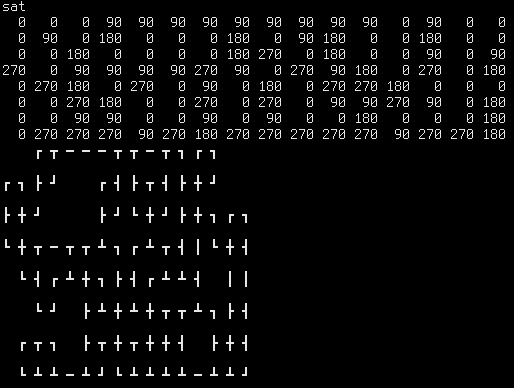
\includegraphics[scale=0.75]{\CURPATH/solver/solver.png}
\caption{Вывод скрипта солвера}
\end{figure}

Это работает $\approx 4$ секунды на моем старом и медленном Intel Atom N455 1.66GHz.
Быстро ли это? Не знаю, но снова вот что действительно круто, это то что мы понятия не имеем о какой-то математической
теории за всем этим, мы просто объявили ячейки, (полу-)стыки и определили отношения между ними.

Теперь следующий вопрос это, сколько здесь возможных решений?
Используя раннее описанный метод (\ref{SMTEnumerate}), я немного изменил скрипт солвера
\footnote{\url{.../solver/solve_pipe_puzzle2.py}} и солвер
сказал что возможно два решения.

Сравним их используя gvimdiff:

\begin{figure}[H]
\centering
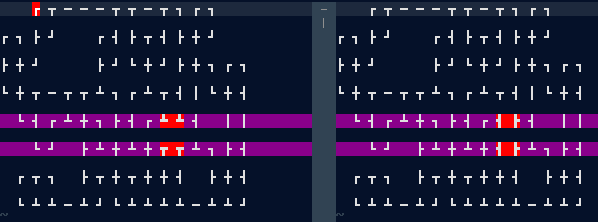
\includegraphics[scale=0.75]{\CURPATH/solver/diff.png}
\caption{Вывод gvimdiff (извините за мой красный курсор в левой части в левом верхнем углу)}
\end{figure}

4 ячейки в середине могут быть ориентированы по-разному.
Видимо, другие головоломки могут также выдавать разные результаты.

P.S.
\textit{Полу-стык} определен как булевый тип.
Но на самом деле, первая версия солвера была написана используя целочисленный тип для полу-стыков,
и 0 использовалось для False и 1 для True.
Я так сделал, потому что хотел более компактный исходный код, без использования длинных слов как ``False'' и ``True''.
И это работало, но медленнее. Вероятно, Z3 работает с булевыми типами быстрее? Лучше?
Так или иначе, я пишу это чтобы отметить, что, если нужно, целочисленный тип можно использовать вместо булевого.


\section{Развлекательная математика и головоломки}

\input{puzzles/sudoku/main_RU}
\input{puzzles/zebra/main_RU}
\input{puzzles/pipe/main_RU}
\input{puzzles/rubik2/failed_SMT/main_RU}
\input{puzzles/rubik2/SAT/main_RU}
\input{puzzles/rubik3/one_face_SMT/main_RU}
%\input{puzzles/numberlink/main_RU}
%\input{puzzles/two_parks_RU}
\input{puzzles/alphametics/main_RU}
%\input{puzzles/2015_AIME_II_Problems_12_RU}
%\input{puzzles/fred/main_RU}
%\input{puzzles/MC/main_RU}
%\input{puzzles/coin_flip/main_RU}
%\input{puzzles/Mock_AIME_2_2006-2007_Problem_8_RU}
%\input{puzzles/2012_AIME_I_Problems_1_RU}
%\input{puzzles/keypad_RU}


\section{Развлекательная математика и головоломки}

\input{puzzles/sudoku/main_RU}
\input{puzzles/zebra/main_RU}
\input{puzzles/pipe/main_RU}
\input{puzzles/rubik2/failed_SMT/main_RU}
\input{puzzles/rubik2/SAT/main_RU}
\input{puzzles/rubik3/one_face_SMT/main_RU}
%\input{puzzles/numberlink/main_RU}
%\input{puzzles/two_parks_RU}
\input{puzzles/alphametics/main_RU}
%\input{puzzles/2015_AIME_II_Problems_12_RU}
%\input{puzzles/fred/main_RU}
%\input{puzzles/MC/main_RU}
%\input{puzzles/coin_flip/main_RU}
%\input{puzzles/Mock_AIME_2_2006-2007_Problem_8_RU}
%\input{puzzles/2012_AIME_I_Problems_1_RU}
%\input{puzzles/keypad_RU}


\section{Развлекательная математика и головоломки}

\input{puzzles/sudoku/main_RU}
\input{puzzles/zebra/main_RU}
\input{puzzles/pipe/main_RU}
\input{puzzles/rubik2/failed_SMT/main_RU}
\input{puzzles/rubik2/SAT/main_RU}
\input{puzzles/rubik3/one_face_SMT/main_RU}
%\input{puzzles/numberlink/main_RU}
%\input{puzzles/two_parks_RU}
\input{puzzles/alphametics/main_RU}
%\input{puzzles/2015_AIME_II_Problems_12_RU}
%\input{puzzles/fred/main_RU}
%\input{puzzles/MC/main_RU}
%\input{puzzles/coin_flip/main_RU}
%\input{puzzles/Mock_AIME_2_2006-2007_Problem_8_RU}
%\input{puzzles/2012_AIME_I_Problems_1_RU}
%\input{puzzles/keypad_RU}


%\section{Развлекательная математика и головоломки}

\input{puzzles/sudoku/main_RU}
\input{puzzles/zebra/main_RU}
\input{puzzles/pipe/main_RU}
\input{puzzles/rubik2/failed_SMT/main_RU}
\input{puzzles/rubik2/SAT/main_RU}
\input{puzzles/rubik3/one_face_SMT/main_RU}
%\input{puzzles/numberlink/main_RU}
%\input{puzzles/two_parks_RU}
\input{puzzles/alphametics/main_RU}
%\input{puzzles/2015_AIME_II_Problems_12_RU}
%\input{puzzles/fred/main_RU}
%\input{puzzles/MC/main_RU}
%\input{puzzles/coin_flip/main_RU}
%\input{puzzles/Mock_AIME_2_2006-2007_Problem_8_RU}
%\input{puzzles/2012_AIME_I_Problems_1_RU}
%\input{puzzles/keypad_RU}


%\input{puzzles/two_parks_RU}
\subsection{Альфаметика}

Согласно Дональду Кнуту, термин ``Альфаметика'' был придуман Дж. Эйч. Аш. Хантером.
Это головоломка: какие десятичные цифры в пределах 0..9 нужно присвоить каждой букве, чтобы это уравнение было справедливо?

\begin{lstlisting}
  SEND
+ MORE
 -----
 MONEY
\end{lstlisting}

Для Z3 это легко:

\lstinputlisting{puzzles/alphametics/alpha.py}

Вывод:

\begin{lstlisting}
sat
[E, = 5,
 S, = 9,
 M, = 1,
 N, = 6,
 D, = 7,
 R, = 8,
 O, = 0,
 Y = 2]
\end{lstlisting}

Вот еще одна, из \ac{TAOCP} том IV (\url{http://www-cs-faculty.stanford.edu/~uno/fasc2b.ps.gz}):

\lstinputlisting{puzzles/alphametics/alpha2.py}

\begin{lstlisting}
sat
[L, = 6,
 S, = 7,
 N, = 2,
 T, = 1,
 I, = 5,
 V = 3,
 A, = 8,
 R, = 9,
 O, = 4,
 TRIO = 1954,
 SONATA, = 742818,
 VIOLA, = 35468,
 VIOLIN, = 354652]
\end{lstlisting}

% TODO URL
Эту головоломку я нашел в примерах pySMT:

\lstinputlisting{puzzles/alphametics/alpha3.py}

\begin{lstlisting}
sat
[D = 5, R = 4, O = 3, E = 8, L = 6, W = 7, H = 2]
\end{lstlisting}

%%% 

Это упражнение Q209 из
[Companion to the Papers of Donald Knuth]\footnote{\url{http://www-cs-faculty.stanford.edu/~knuth/cp.html}}.

\begin{lstlisting}
 KNIFE
  FORK
 SPOON
  SOUP
------
SUPPER
\end{lstlisting}

В целях упрощения, я добавил ф-цию (list\_to\_expr()):

\lstinputlisting{puzzles/alphametics/alpha4.py}

\begin{lstlisting}
sat
[K = 7,
 N = 4,
 R = 9,
 I = 1,
 E = 6,
 S = 0,
 O = 3,
 F = 5,
 U = 8,
 P = 2,
 SUPPER = 82269,
 SOUP = 382,
 SPOON = 2334,
 FORK = 5397,
 KNIFE = 74156]
\end{lstlisting}

S это 0, так что значение SUPPER начинается с (убранного) нуля. Скажем так, нам это не нравится.
Добавим это, чтобы это исправить:

\begin{lstlisting}
s.add(S!=0)
\end{lstlisting}

\begin{lstlisting}
sat
[K = 8,
 N = 4,
 R = 3,
 I = 7,
 E = 6,
 S = 1,
 O = 9,
 F = 2,
 U = 0,
 P = 5,
 SUPPER = 105563,
 SOUP = 1905,
 SPOON = 15994,
 FORK = 2938,
 KNIFE = 84726]
\end{lstlisting}

\paragraph{Создание своей собственной головоломки}

Вот проблема: есть только 10 букв, но как их выбрать из числа слов?
Мы можем использовать Z3 для этого:

\lstinputlisting{puzzles/alphametics/gen.py}

Это первая сгенерированная головоломка:

\begin{lstlisting}
sat
EGGS
JELLY
LUNCH
C 5
E 6
G 3
H 7
J 0
L 1
N 4
S 8
U 2
Y 9
\end{lstlisting}

Что если мы хотим, чтобы слово ``CAKE'' присутствовало в числе ``слагаемых''?

Добавим это:

\begin{lstlisting}
s.add(word_used[words.index('CAKE')])
\end{lstlisting}

\begin{lstlisting}
sat
CAKE
TEA
LUNCH
A 8
C 3
E 1
H 9
J 6
K 2
L 0
N 5
T 7
U 4
\end{lstlisting}

Добавим это:

\begin{lstlisting}
s.add(word_used[words.index('EGGS')])
\end{lstlisting}

Теперь оно может найти пару к EGGS:

\begin{lstlisting}
sat
EGGS
HONEY
LUNCH
C 6
E 7
G 9
H 4
L 5
N 8
O 2
S 3
U 0
Y 1
\end{lstlisting}

\paragraph{Файлы}

\url{https://github.com/DennisYurichev/...}




%\input{puzzles/2015_AIME_II_Problems_12_RU}
%\section{Развлекательная математика и головоломки}

\input{puzzles/sudoku/main_RU}
\input{puzzles/zebra/main_RU}
\input{puzzles/pipe/main_RU}
\input{puzzles/rubik2/failed_SMT/main_RU}
\input{puzzles/rubik2/SAT/main_RU}
\input{puzzles/rubik3/one_face_SMT/main_RU}
%\input{puzzles/numberlink/main_RU}
%\input{puzzles/two_parks_RU}
\input{puzzles/alphametics/main_RU}
%\input{puzzles/2015_AIME_II_Problems_12_RU}
%\input{puzzles/fred/main_RU}
%\input{puzzles/MC/main_RU}
%\input{puzzles/coin_flip/main_RU}
%\input{puzzles/Mock_AIME_2_2006-2007_Problem_8_RU}
%\input{puzzles/2012_AIME_I_Problems_1_RU}
%\input{puzzles/keypad_RU}


%\section{Развлекательная математика и головоломки}

\input{puzzles/sudoku/main_RU}
\input{puzzles/zebra/main_RU}
\input{puzzles/pipe/main_RU}
\input{puzzles/rubik2/failed_SMT/main_RU}
\input{puzzles/rubik2/SAT/main_RU}
\input{puzzles/rubik3/one_face_SMT/main_RU}
%\input{puzzles/numberlink/main_RU}
%\input{puzzles/two_parks_RU}
\input{puzzles/alphametics/main_RU}
%\input{puzzles/2015_AIME_II_Problems_12_RU}
%\input{puzzles/fred/main_RU}
%\input{puzzles/MC/main_RU}
%\input{puzzles/coin_flip/main_RU}
%\input{puzzles/Mock_AIME_2_2006-2007_Problem_8_RU}
%\input{puzzles/2012_AIME_I_Problems_1_RU}
%\input{puzzles/keypad_RU}


%\section{Развлекательная математика и головоломки}

\input{puzzles/sudoku/main_RU}
\input{puzzles/zebra/main_RU}
\input{puzzles/pipe/main_RU}
\input{puzzles/rubik2/failed_SMT/main_RU}
\input{puzzles/rubik2/SAT/main_RU}
\input{puzzles/rubik3/one_face_SMT/main_RU}
%\input{puzzles/numberlink/main_RU}
%\input{puzzles/two_parks_RU}
\input{puzzles/alphametics/main_RU}
%\input{puzzles/2015_AIME_II_Problems_12_RU}
%\input{puzzles/fred/main_RU}
%\input{puzzles/MC/main_RU}
%\input{puzzles/coin_flip/main_RU}
%\input{puzzles/Mock_AIME_2_2006-2007_Problem_8_RU}
%\input{puzzles/2012_AIME_I_Problems_1_RU}
%\input{puzzles/keypad_RU}


%\input{puzzles/Mock_AIME_2_2006-2007_Problem_8_RU}
%\input{puzzles/2012_AIME_I_Problems_1_RU}
%\input{puzzles/keypad_RU}


%\input{puzzles/two_parks_RU}
\subsection{Альфаметика}

Согласно Дональду Кнуту, термин ``Альфаметика'' был придуман Дж. Эйч. Аш. Хантером.
Это головоломка: какие десятичные цифры в пределах 0..9 нужно присвоить каждой букве, чтобы это уравнение было справедливо?

\begin{lstlisting}
  SEND
+ MORE
 -----
 MONEY
\end{lstlisting}

Для Z3 это легко:

\lstinputlisting{puzzles/alphametics/alpha.py}

Вывод:

\begin{lstlisting}
sat
[E, = 5,
 S, = 9,
 M, = 1,
 N, = 6,
 D, = 7,
 R, = 8,
 O, = 0,
 Y = 2]
\end{lstlisting}

Вот еще одна, из \ac{TAOCP} том IV (\url{http://www-cs-faculty.stanford.edu/~uno/fasc2b.ps.gz}):

\lstinputlisting{puzzles/alphametics/alpha2.py}

\begin{lstlisting}
sat
[L, = 6,
 S, = 7,
 N, = 2,
 T, = 1,
 I, = 5,
 V = 3,
 A, = 8,
 R, = 9,
 O, = 4,
 TRIO = 1954,
 SONATA, = 742818,
 VIOLA, = 35468,
 VIOLIN, = 354652]
\end{lstlisting}

% TODO URL
Эту головоломку я нашел в примерах pySMT:

\lstinputlisting{puzzles/alphametics/alpha3.py}

\begin{lstlisting}
sat
[D = 5, R = 4, O = 3, E = 8, L = 6, W = 7, H = 2]
\end{lstlisting}

%%% 

Это упражнение Q209 из
[Companion to the Papers of Donald Knuth]\footnote{\url{http://www-cs-faculty.stanford.edu/~knuth/cp.html}}.

\begin{lstlisting}
 KNIFE
  FORK
 SPOON
  SOUP
------
SUPPER
\end{lstlisting}

В целях упрощения, я добавил ф-цию (list\_to\_expr()):

\lstinputlisting{puzzles/alphametics/alpha4.py}

\begin{lstlisting}
sat
[K = 7,
 N = 4,
 R = 9,
 I = 1,
 E = 6,
 S = 0,
 O = 3,
 F = 5,
 U = 8,
 P = 2,
 SUPPER = 82269,
 SOUP = 382,
 SPOON = 2334,
 FORK = 5397,
 KNIFE = 74156]
\end{lstlisting}

S это 0, так что значение SUPPER начинается с (убранного) нуля. Скажем так, нам это не нравится.
Добавим это, чтобы это исправить:

\begin{lstlisting}
s.add(S!=0)
\end{lstlisting}

\begin{lstlisting}
sat
[K = 8,
 N = 4,
 R = 3,
 I = 7,
 E = 6,
 S = 1,
 O = 9,
 F = 2,
 U = 0,
 P = 5,
 SUPPER = 105563,
 SOUP = 1905,
 SPOON = 15994,
 FORK = 2938,
 KNIFE = 84726]
\end{lstlisting}

\paragraph{Создание своей собственной головоломки}

Вот проблема: есть только 10 букв, но как их выбрать из числа слов?
Мы можем использовать Z3 для этого:

\lstinputlisting{puzzles/alphametics/gen.py}

Это первая сгенерированная головоломка:

\begin{lstlisting}
sat
EGGS
JELLY
LUNCH
C 5
E 6
G 3
H 7
J 0
L 1
N 4
S 8
U 2
Y 9
\end{lstlisting}

Что если мы хотим, чтобы слово ``CAKE'' присутствовало в числе ``слагаемых''?

Добавим это:

\begin{lstlisting}
s.add(word_used[words.index('CAKE')])
\end{lstlisting}

\begin{lstlisting}
sat
CAKE
TEA
LUNCH
A 8
C 3
E 1
H 9
J 6
K 2
L 0
N 5
T 7
U 4
\end{lstlisting}

Добавим это:

\begin{lstlisting}
s.add(word_used[words.index('EGGS')])
\end{lstlisting}

Теперь оно может найти пару к EGGS:

\begin{lstlisting}
sat
EGGS
HONEY
LUNCH
C 6
E 7
G 9
H 4
L 5
N 8
O 2
S 3
U 0
Y 1
\end{lstlisting}

\paragraph{Файлы}

\url{https://github.com/DennisYurichev/...}




%\input{puzzles/2015_AIME_II_Problems_12_RU}
%\section{Развлекательная математика и головоломки}

\subsection{Судоку}

Головоломка Судоку это решетка 9*9, некоторые ячейки заполнены значениями, некоторые пустые:

% copypasted from http://www.texample.net/tikz/examples/sudoku/
\newcounter{row}
\newcounter{col}

\newcommand\setrow[9]{
  \setcounter{col}{1}
  \foreach \n in {#1, #2, #3, #4, #5, #6, #7, #8, #9} {
    \edef\x{\value{col} - 0.5}
    \edef\y{9.5 - \value{row}}
    \node[anchor=center] at (\x, \y) {\n};
    \stepcounter{col}
  }
  \stepcounter{row}
}

\begin{center}
\begin{tikzpicture}[scale=.7]
  \begin{scope}
    \draw (0, 0) grid (9, 9);
    \draw[very thick, scale=3] (0, 0) grid (3, 3);

    \setcounter{row}{1}
    \setrow { }{ }{5}  {3}{ }{ }  { }{ }{ }
    \setrow {8}{ }{ }  { }{ }{ }  { }{2}{ }
    \setrow { }{7}{ }  { }{1}{ }  {5}{ }{ }

    \setrow {4}{ }{ }  { }{ }{5}  {3}{ }{ }
    \setrow { }{1}{ }  { }{7}{ }  { }{ }{6}
    \setrow { }{ }{3}  {2}{ }{ }  { }{8}{ }

    \setrow { }{6}{ }  {5}{ }{ }  { }{ }{9}
    \setrow { }{ }{4}  { }{ }{ }  { }{3}{ }
    \setrow { }{ }{ }  { }{ }{9}  {7}{ }{ }

    \node[anchor=center] at (4.5, -0.5) {Нерешенная Судоку};
  \end{scope}
\end{tikzpicture}
\end{center}

Числа в каждом ряду должны быть уникальными, т.е., каждый ряд должен содержать 9 чисел в пределах 1..9 без повторений.
Та же история и для каждого столбца и каждого квадрата 3*3.

Головоломка представляет собой хороший кандидат, на котором можно попробовать \ac{SMT}-солвер, потому что это,
в общем-то, просто нерешенная система уравнений.

\input{puzzles/sudoku/1/main_RU}
%\input{puzzles/sudoku/GT/main_RU}
%\input{puzzles/sudoku/killer/main_RU}
\input{puzzles/sudoku/KLEE/main_RU}
\input{puzzles/sudoku/SAT/main_RU}


\subsection{Головоломка зебры (\ac{AKA} Загадка Эйнштейна)}

\input{puzzles/zebra/SMT/main_RU}
\input{puzzles/zebra/KLEE/main_RU}
\input{puzzles/zebra/SAT/main_RU}


\subsection{Решение головоломки ``трубы'' используя Z3 SMT-солвер}

\renewcommand{\CURPATH}{puzzles/pipe}

Головоломка ``трубы'' это популярная головоломка (просто погуглите ``pipe puzzle'' и посмотрите на картинки).

Вот как выглядит головоломка в разобранном виде:

\begin{figure}[H]
\label{fig:pipe_shuffled}
\centering
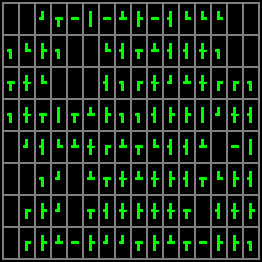
\includegraphics[scale=0.75]{\CURPATH/shuffled.png}
\caption{Разобранная головоломка}
\end{figure}

\dots и собранная:

\begin{figure}[H]
\label{fig:pipe_solved}
\centering
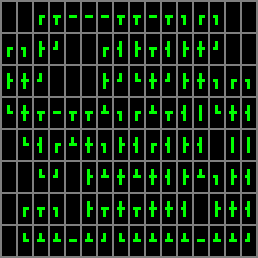
\includegraphics[scale=0.75]{\CURPATH/solved.png}
\caption{Собранная головоломка}
\end{figure}

Попробуем найти способ собрать её.

\subsubsection{Создание}

В начале, нужно её создать.
Вот простая идея.
Возьем массив ячеек 8*16.
Каждая ячейка может содержать какой-то тип блока.
Между ячейками есть стыки:

\input{\CURPATH/pipe_gen.tex}

Синие линии это горизонтальные стыки, красные линии это вертикальные стыки.
Мы просто случайно выставляем каждый стык в 0/false (отсутствует) или 1/true (присутствует).

После этого, теперь легко найти тип каждой ячейки.
А это:

\newcommand{\HeaderColor}{\cellcolor{blue!25}}
\begin{center}
\begin{longtable}{ | l | l | l | l | }
\hline
\HeaderColor стыки & \HeaderColor наше внутреннее название & \HeaderColor угол & \HeaderColor символ \\
\hline
0	&type 0		&	0$^{\circ}$	& (пробел)	\\
2	&type 2a	&	0$^{\circ}$	& \pmboxdrawuni{2503} \\ % ┃
2	&type 2a	&	90$^{\circ}$	& \pmboxdrawuni{2501} \\ % ━
2	&type 2b	&	0$^{\circ}$	& \pmboxdrawuni{250F} \\ % ┏
2	&type 2b	&	90$^{\circ}$	& \pmboxdrawuni{2513} \\ % ┓
2	&type 2b	&	180$^{\circ}$	& \pmboxdrawuni{251B} \\ % ┛
2	&type 2b	&	270$^{\circ}$	& \pmboxdrawuni{2517} \\ % ┗
3	&type 3		&	0$^{\circ}$	& \pmboxdrawuni{2523} \\ % ┣
3 	&type 3		&	90$^{\circ}$	& \pmboxdrawuni{2533} \\ % ┳
3	&type 3		&	180$^{\circ}$	& \pmboxdrawuni{252B} \\ % ┫
3	&type 3		&	270$^{\circ}$	& \pmboxdrawuni{253B} \\ % ┻
4	&type 4		&	0$^{\circ}$	& \pmboxdrawuni{254B} \\ % ╋
\hline
\end{longtable}
\end{center}

\textit{Висящие} стыки могут присутствовать на первой стадии (т.е., ячейки только с одним стыком), но они удалются
рекурсивно, и эти ячейки преобразуются в пустые ячейки.
Так что, в самом конце, все ячейки имеют минимум 2 стыка, и вся эта сантехническая система не имеет связей с внешним миром ---
я надеюсь, из-за этого станет немного проще.

Исходник генератора на Си здесь: \url{.../pipe/generator}.
Все вертикальные стыки хранятся в глобальном массиве \textit{hjoints[]} и вертикальные в \textit{vjoints[]}.

Программа на Си генерирует ANSI-раскрашенный вывод, как это было показано выше
(\ref{fig:pipe_shuffled}, \ref{fig:pipe_solved}) плюс массив типов для каждой ячейки, но без информации об углах:

\begin{lstlisting}[label=init_cells]
[
["0", "0", "2b", "3", "2a", "2a", "2a", "3", "3", "2a", "3", "2b", "2b", "2b", "0", "0"],
["2b", "2b", "3", "2b", "0", "0", "2b", "3", "3", "3", "3", "3", "4", "2b", "0", "0"],
["3", "4", "2b", "0", "0", "0", "3", "2b", "2b", "4", "2b", "3", "4", "2b", "2b", "2b"],
["2b", "4", "3", "2a", "3", "3", "3", "2b", "2b", "3", "3", "3", "2a", "2b", "4", "3"],
["0", "2b", "3", "2b", "3", "4", "2b", "3", "3", "2b", "3", "3", "3", "0", "2a", "2a"],
["0", "0", "2b", "2b", "0", "3", "3", "4", "3", "4", "3", "3", "3", "2b", "3", "3"],
["0", "2b", "3", "2b", "0", "3", "3", "4", "3", "4", "4", "3", "0", "3", "4", "3"],
["0", "2b", "3", "3", "2a", "3", "2b", "2b", "3", "3", "3", "3", "2a", "3", "3", "2b"],
]
\end{lstlisting}

\subsubsection{Решение}

Прежде всего, мы будем работать с массивом ячеек 8*16, где каждый элемент имеет 4 бита:
``T'' (top/верх),
``B'' (bottom/низ),
``L'' (left/лево),
``R'' (right/право).
Каждый бит представляет собой половину стыка.

\input{\CURPATH/pipe_solve.tex}

Теперь определяем массив для каждого из четырех полустыков + информация об угле:

\begin{lstlisting}
HEIGHT=8
WIDTH=16

# if T/B/R/L is Bool instead of Int, Z3 solver will work faster
T=[[Bool('cell_%d_%d_top' % (r, c)) for c in range(WIDTH)] for r in range(HEIGHT)]
B=[[Bool('cell_%d_%d_bottom' % (r, c)) for c in range(WIDTH)] for r in range(HEIGHT)]
R=[[Bool('cell_%d_%d_right' % (r, c)) for c in range(WIDTH)] for r in range(HEIGHT)]
L=[[Bool('cell_%d_%d_left' % (r, c)) for c in range(WIDTH)] for r in range(HEIGHT)]
A=[[Int('cell_%d_%d_angle' % (r, c)) for c in range(WIDTH)] for r in range(HEIGHT)]
\end{lstlisting}

Мы знаем, что если каждый из полустыков присутствует, ответный полустык также должен присутствовать, и наоборот. 
Определяем всё это используя эти констрайнты:

\begin{lstlisting}
# shorthand variables for True and False:
t=True
f=False

# "top" of each cell must be equal to "bottom" of the cell above
# "bottom" of each cell must be equal to "top" of the cell below
# "left" of each cell must be equal to "right" of the cell at left
# "right" of each cell must be equal to "left" of the cell at right
for r in range(HEIGHT):
    for c in range(WIDTH):
        if r!=0:
            s.add(T[r][c]==B[r-1][c])
        if r!=HEIGHT-1:
            s.add(B[r][c]==T[r+1][c])
        if c!=0:
            s.add(L[r][c]==R[r][c-1])
        if c!=WIDTH-1:
            s.add(R[r][c]==L[r][c+1])

# "left" of each cell of first column shouldn't have any connection
# so is "right" of each cell of the last column
for r in range(HEIGHT):
    s.add(L[r][0]==f)
    s.add(R[r][WIDTH-1]==f)

# "top" of each cell of the first row shouldn't have any connection
# so is "bottom" of each cell of the last row
for c in range(WIDTH):
    s.add(T[0][c]==f)
    s.add(B[HEIGHT-1][c]==f)
\end{lstlisting}

Теперь перебираем все ячейки в изначальном массиве (\ref{init_cells}).
Первые две ячейки здесь пустые. И третья имеет тип ``2b''.
Это ``\pmboxdrawuni{250F}'' % ┏
и его можно ориентировать четырьмя разными способами.
И если её угол это 0$^{\circ}$, верхний и правый полустыки присутствуют, остальные отсутствуют.
Если он имеет угол 90$^{\circ}$, он выглядит как 
``\pmboxdrawuni{2513}'', % ┓
и верхник и левый полустыки присутствуют, остальные отсутствуют.

На обычном русском языке: ``если ячейка этого типа имеет угол 0$^{\circ}$, вот эти полустыки должны присутствовать \textbf{ИЛИ}
если она имеет угол 90$^{\circ}$, эти полустыки должны присутствовать, \textbf{ИЛИ}, итд, итд.''

Точно также, мы определяем эти правила для всех типов и всех возможных углов:

\begin{lstlisting}
for r in range(HEIGHT):
    for c in range(WIDTH):
        ty=cells_type[r][c]

        if ty=="0":
            s.add(A[r][c]==f)
            s.add(T[r][c]==f, B[r][c]==f, L[r][c]==f, R[r][c]==f)

        if ty=="2a":
            s.add(Or(And(A[r][c]==0, L[r][c]==f, R[r][c]==f, T[r][c]==t, B[r][c]==t),   # §\pmboxdrawuni{2503}§
                    And(A[r][c]==90, L[r][c]==t, R[r][c]==t, T[r][c]==f, B[r][c]==f)))  # §\pmboxdrawuni{2501}§

        if ty=="2b":
            s.add(Or(And(A[r][c]==0, L[r][c]==f, R[r][c]==t, T[r][c]==f, B[r][c]==t),   # §\pmboxdrawuni{250F}§
                    And(A[r][c]==90, L[r][c]==t, R[r][c]==f, T[r][c]==f, B[r][c]==t),   # §\pmboxdrawuni{2513}§
                    And(A[r][c]==180, L[r][c]==t, R[r][c]==f, T[r][c]==t, B[r][c]==f),  # §\pmboxdrawuni{251B}§
                    And(A[r][c]==270, L[r][c]==f, R[r][c]==t, T[r][c]==t, B[r][c]==f))) # §\pmboxdrawuni{2517}§
	
        if ty=="3":
            s.add(Or(And(A[r][c]==0, L[r][c]==f, R[r][c]==t, T[r][c]==t, B[r][c]==t),   # §\pmboxdrawuni{2523}§
                    And(A[r][c]==90, L[r][c]==t, R[r][c]==t, T[r][c]==f, B[r][c]==t),   # §\pmboxdrawuni{2533}§
                    And(A[r][c]==180, L[r][c]==t, R[r][c]==f, T[r][c]==t, B[r][c]==t),  # §\pmboxdrawuni{252B}§
                    And(A[r][c]==270, L[r][c]==t, R[r][c]==t, T[r][c]==t, B[r][c]==f))) # §\pmboxdrawuni{253B}§

        if ty=="4":
            s.add(A[r][c]==0)
            s.add(T[r][c]==t, B[r][c]==t, L[r][c]==t, R[r][c]==t) # §\pmboxdrawuni{254B}§
\end{lstlisting}

Полный исходник здесь: \url{.../solver/solve_pipe_puzzle1.py}.

Получается такой результат (выводит угол для каждой ячейки и (псевдо)графическое представление):

\begin{figure}[H]
\centering
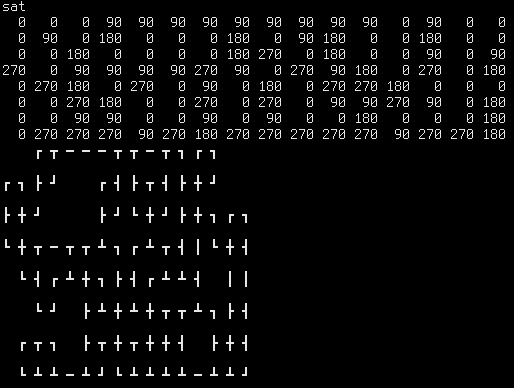
\includegraphics[scale=0.75]{\CURPATH/solver/solver.png}
\caption{Вывод скрипта солвера}
\end{figure}

Это работает $\approx 4$ секунды на моем старом и медленном Intel Atom N455 1.66GHz.
Быстро ли это? Не знаю, но снова вот что действительно круто, это то что мы понятия не имеем о какой-то математической
теории за всем этим, мы просто объявили ячейки, (полу-)стыки и определили отношения между ними.

Теперь следующий вопрос это, сколько здесь возможных решений?
Используя раннее описанный метод (\ref{SMTEnumerate}), я немного изменил скрипт солвера
\footnote{\url{.../solver/solve_pipe_puzzle2.py}} и солвер
сказал что возможно два решения.

Сравним их используя gvimdiff:

\begin{figure}[H]
\centering
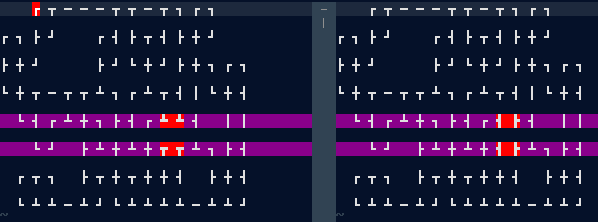
\includegraphics[scale=0.75]{\CURPATH/solver/diff.png}
\caption{Вывод gvimdiff (извините за мой красный курсор в левой части в левом верхнем углу)}
\end{figure}

4 ячейки в середине могут быть ориентированы по-разному.
Видимо, другие головоломки могут также выдавать разные результаты.

P.S.
\textit{Полу-стык} определен как булевый тип.
Но на самом деле, первая версия солвера была написана используя целочисленный тип для полу-стыков,
и 0 использовалось для False и 1 для True.
Я так сделал, потому что хотел более компактный исходный код, без использования длинных слов как ``False'' и ``True''.
И это работало, но медленнее. Вероятно, Z3 работает с булевыми типами быстрее? Лучше?
Так или иначе, я пишу это чтобы отметить, что, если нужно, целочисленный тип можно использовать вместо булевого.


\section{Развлекательная математика и головоломки}

\input{puzzles/sudoku/main_RU}
\input{puzzles/zebra/main_RU}
\input{puzzles/pipe/main_RU}
\input{puzzles/rubik2/failed_SMT/main_RU}
\input{puzzles/rubik2/SAT/main_RU}
\input{puzzles/rubik3/one_face_SMT/main_RU}
%\input{puzzles/numberlink/main_RU}
%\input{puzzles/two_parks_RU}
\input{puzzles/alphametics/main_RU}
%\input{puzzles/2015_AIME_II_Problems_12_RU}
%\input{puzzles/fred/main_RU}
%\input{puzzles/MC/main_RU}
%\input{puzzles/coin_flip/main_RU}
%\input{puzzles/Mock_AIME_2_2006-2007_Problem_8_RU}
%\input{puzzles/2012_AIME_I_Problems_1_RU}
%\input{puzzles/keypad_RU}


\section{Развлекательная математика и головоломки}

\input{puzzles/sudoku/main_RU}
\input{puzzles/zebra/main_RU}
\input{puzzles/pipe/main_RU}
\input{puzzles/rubik2/failed_SMT/main_RU}
\input{puzzles/rubik2/SAT/main_RU}
\input{puzzles/rubik3/one_face_SMT/main_RU}
%\input{puzzles/numberlink/main_RU}
%\input{puzzles/two_parks_RU}
\input{puzzles/alphametics/main_RU}
%\input{puzzles/2015_AIME_II_Problems_12_RU}
%\input{puzzles/fred/main_RU}
%\input{puzzles/MC/main_RU}
%\input{puzzles/coin_flip/main_RU}
%\input{puzzles/Mock_AIME_2_2006-2007_Problem_8_RU}
%\input{puzzles/2012_AIME_I_Problems_1_RU}
%\input{puzzles/keypad_RU}


\section{Развлекательная математика и головоломки}

\input{puzzles/sudoku/main_RU}
\input{puzzles/zebra/main_RU}
\input{puzzles/pipe/main_RU}
\input{puzzles/rubik2/failed_SMT/main_RU}
\input{puzzles/rubik2/SAT/main_RU}
\input{puzzles/rubik3/one_face_SMT/main_RU}
%\input{puzzles/numberlink/main_RU}
%\input{puzzles/two_parks_RU}
\input{puzzles/alphametics/main_RU}
%\input{puzzles/2015_AIME_II_Problems_12_RU}
%\input{puzzles/fred/main_RU}
%\input{puzzles/MC/main_RU}
%\input{puzzles/coin_flip/main_RU}
%\input{puzzles/Mock_AIME_2_2006-2007_Problem_8_RU}
%\input{puzzles/2012_AIME_I_Problems_1_RU}
%\input{puzzles/keypad_RU}


%\section{Развлекательная математика и головоломки}

\input{puzzles/sudoku/main_RU}
\input{puzzles/zebra/main_RU}
\input{puzzles/pipe/main_RU}
\input{puzzles/rubik2/failed_SMT/main_RU}
\input{puzzles/rubik2/SAT/main_RU}
\input{puzzles/rubik3/one_face_SMT/main_RU}
%\input{puzzles/numberlink/main_RU}
%\input{puzzles/two_parks_RU}
\input{puzzles/alphametics/main_RU}
%\input{puzzles/2015_AIME_II_Problems_12_RU}
%\input{puzzles/fred/main_RU}
%\input{puzzles/MC/main_RU}
%\input{puzzles/coin_flip/main_RU}
%\input{puzzles/Mock_AIME_2_2006-2007_Problem_8_RU}
%\input{puzzles/2012_AIME_I_Problems_1_RU}
%\input{puzzles/keypad_RU}


%\input{puzzles/two_parks_RU}
\subsection{Альфаметика}

Согласно Дональду Кнуту, термин ``Альфаметика'' был придуман Дж. Эйч. Аш. Хантером.
Это головоломка: какие десятичные цифры в пределах 0..9 нужно присвоить каждой букве, чтобы это уравнение было справедливо?

\begin{lstlisting}
  SEND
+ MORE
 -----
 MONEY
\end{lstlisting}

Для Z3 это легко:

\lstinputlisting{puzzles/alphametics/alpha.py}

Вывод:

\begin{lstlisting}
sat
[E, = 5,
 S, = 9,
 M, = 1,
 N, = 6,
 D, = 7,
 R, = 8,
 O, = 0,
 Y = 2]
\end{lstlisting}

Вот еще одна, из \ac{TAOCP} том IV (\url{http://www-cs-faculty.stanford.edu/~uno/fasc2b.ps.gz}):

\lstinputlisting{puzzles/alphametics/alpha2.py}

\begin{lstlisting}
sat
[L, = 6,
 S, = 7,
 N, = 2,
 T, = 1,
 I, = 5,
 V = 3,
 A, = 8,
 R, = 9,
 O, = 4,
 TRIO = 1954,
 SONATA, = 742818,
 VIOLA, = 35468,
 VIOLIN, = 354652]
\end{lstlisting}

% TODO URL
Эту головоломку я нашел в примерах pySMT:

\lstinputlisting{puzzles/alphametics/alpha3.py}

\begin{lstlisting}
sat
[D = 5, R = 4, O = 3, E = 8, L = 6, W = 7, H = 2]
\end{lstlisting}

%%% 

Это упражнение Q209 из
[Companion to the Papers of Donald Knuth]\footnote{\url{http://www-cs-faculty.stanford.edu/~knuth/cp.html}}.

\begin{lstlisting}
 KNIFE
  FORK
 SPOON
  SOUP
------
SUPPER
\end{lstlisting}

В целях упрощения, я добавил ф-цию (list\_to\_expr()):

\lstinputlisting{puzzles/alphametics/alpha4.py}

\begin{lstlisting}
sat
[K = 7,
 N = 4,
 R = 9,
 I = 1,
 E = 6,
 S = 0,
 O = 3,
 F = 5,
 U = 8,
 P = 2,
 SUPPER = 82269,
 SOUP = 382,
 SPOON = 2334,
 FORK = 5397,
 KNIFE = 74156]
\end{lstlisting}

S это 0, так что значение SUPPER начинается с (убранного) нуля. Скажем так, нам это не нравится.
Добавим это, чтобы это исправить:

\begin{lstlisting}
s.add(S!=0)
\end{lstlisting}

\begin{lstlisting}
sat
[K = 8,
 N = 4,
 R = 3,
 I = 7,
 E = 6,
 S = 1,
 O = 9,
 F = 2,
 U = 0,
 P = 5,
 SUPPER = 105563,
 SOUP = 1905,
 SPOON = 15994,
 FORK = 2938,
 KNIFE = 84726]
\end{lstlisting}

\paragraph{Создание своей собственной головоломки}

Вот проблема: есть только 10 букв, но как их выбрать из числа слов?
Мы можем использовать Z3 для этого:

\lstinputlisting{puzzles/alphametics/gen.py}

Это первая сгенерированная головоломка:

\begin{lstlisting}
sat
EGGS
JELLY
LUNCH
C 5
E 6
G 3
H 7
J 0
L 1
N 4
S 8
U 2
Y 9
\end{lstlisting}

Что если мы хотим, чтобы слово ``CAKE'' присутствовало в числе ``слагаемых''?

Добавим это:

\begin{lstlisting}
s.add(word_used[words.index('CAKE')])
\end{lstlisting}

\begin{lstlisting}
sat
CAKE
TEA
LUNCH
A 8
C 3
E 1
H 9
J 6
K 2
L 0
N 5
T 7
U 4
\end{lstlisting}

Добавим это:

\begin{lstlisting}
s.add(word_used[words.index('EGGS')])
\end{lstlisting}

Теперь оно может найти пару к EGGS:

\begin{lstlisting}
sat
EGGS
HONEY
LUNCH
C 6
E 7
G 9
H 4
L 5
N 8
O 2
S 3
U 0
Y 1
\end{lstlisting}

\paragraph{Файлы}

\url{https://github.com/DennisYurichev/...}




%\input{puzzles/2015_AIME_II_Problems_12_RU}
%\section{Развлекательная математика и головоломки}

\input{puzzles/sudoku/main_RU}
\input{puzzles/zebra/main_RU}
\input{puzzles/pipe/main_RU}
\input{puzzles/rubik2/failed_SMT/main_RU}
\input{puzzles/rubik2/SAT/main_RU}
\input{puzzles/rubik3/one_face_SMT/main_RU}
%\input{puzzles/numberlink/main_RU}
%\input{puzzles/two_parks_RU}
\input{puzzles/alphametics/main_RU}
%\input{puzzles/2015_AIME_II_Problems_12_RU}
%\input{puzzles/fred/main_RU}
%\input{puzzles/MC/main_RU}
%\input{puzzles/coin_flip/main_RU}
%\input{puzzles/Mock_AIME_2_2006-2007_Problem_8_RU}
%\input{puzzles/2012_AIME_I_Problems_1_RU}
%\input{puzzles/keypad_RU}


%\section{Развлекательная математика и головоломки}

\input{puzzles/sudoku/main_RU}
\input{puzzles/zebra/main_RU}
\input{puzzles/pipe/main_RU}
\input{puzzles/rubik2/failed_SMT/main_RU}
\input{puzzles/rubik2/SAT/main_RU}
\input{puzzles/rubik3/one_face_SMT/main_RU}
%\input{puzzles/numberlink/main_RU}
%\input{puzzles/two_parks_RU}
\input{puzzles/alphametics/main_RU}
%\input{puzzles/2015_AIME_II_Problems_12_RU}
%\input{puzzles/fred/main_RU}
%\input{puzzles/MC/main_RU}
%\input{puzzles/coin_flip/main_RU}
%\input{puzzles/Mock_AIME_2_2006-2007_Problem_8_RU}
%\input{puzzles/2012_AIME_I_Problems_1_RU}
%\input{puzzles/keypad_RU}


%\section{Развлекательная математика и головоломки}

\input{puzzles/sudoku/main_RU}
\input{puzzles/zebra/main_RU}
\input{puzzles/pipe/main_RU}
\input{puzzles/rubik2/failed_SMT/main_RU}
\input{puzzles/rubik2/SAT/main_RU}
\input{puzzles/rubik3/one_face_SMT/main_RU}
%\input{puzzles/numberlink/main_RU}
%\input{puzzles/two_parks_RU}
\input{puzzles/alphametics/main_RU}
%\input{puzzles/2015_AIME_II_Problems_12_RU}
%\input{puzzles/fred/main_RU}
%\input{puzzles/MC/main_RU}
%\input{puzzles/coin_flip/main_RU}
%\input{puzzles/Mock_AIME_2_2006-2007_Problem_8_RU}
%\input{puzzles/2012_AIME_I_Problems_1_RU}
%\input{puzzles/keypad_RU}


%\input{puzzles/Mock_AIME_2_2006-2007_Problem_8_RU}
%\input{puzzles/2012_AIME_I_Problems_1_RU}
%\input{puzzles/keypad_RU}


%\section{Развлекательная математика и головоломки}

\subsection{Судоку}

Головоломка Судоку это решетка 9*9, некоторые ячейки заполнены значениями, некоторые пустые:

% copypasted from http://www.texample.net/tikz/examples/sudoku/
\newcounter{row}
\newcounter{col}

\newcommand\setrow[9]{
  \setcounter{col}{1}
  \foreach \n in {#1, #2, #3, #4, #5, #6, #7, #8, #9} {
    \edef\x{\value{col} - 0.5}
    \edef\y{9.5 - \value{row}}
    \node[anchor=center] at (\x, \y) {\n};
    \stepcounter{col}
  }
  \stepcounter{row}
}

\begin{center}
\begin{tikzpicture}[scale=.7]
  \begin{scope}
    \draw (0, 0) grid (9, 9);
    \draw[very thick, scale=3] (0, 0) grid (3, 3);

    \setcounter{row}{1}
    \setrow { }{ }{5}  {3}{ }{ }  { }{ }{ }
    \setrow {8}{ }{ }  { }{ }{ }  { }{2}{ }
    \setrow { }{7}{ }  { }{1}{ }  {5}{ }{ }

    \setrow {4}{ }{ }  { }{ }{5}  {3}{ }{ }
    \setrow { }{1}{ }  { }{7}{ }  { }{ }{6}
    \setrow { }{ }{3}  {2}{ }{ }  { }{8}{ }

    \setrow { }{6}{ }  {5}{ }{ }  { }{ }{9}
    \setrow { }{ }{4}  { }{ }{ }  { }{3}{ }
    \setrow { }{ }{ }  { }{ }{9}  {7}{ }{ }

    \node[anchor=center] at (4.5, -0.5) {Нерешенная Судоку};
  \end{scope}
\end{tikzpicture}
\end{center}

Числа в каждом ряду должны быть уникальными, т.е., каждый ряд должен содержать 9 чисел в пределах 1..9 без повторений.
Та же история и для каждого столбца и каждого квадрата 3*3.

Головоломка представляет собой хороший кандидат, на котором можно попробовать \ac{SMT}-солвер, потому что это,
в общем-то, просто нерешенная система уравнений.

\input{puzzles/sudoku/1/main_RU}
%\input{puzzles/sudoku/GT/main_RU}
%\input{puzzles/sudoku/killer/main_RU}
\input{puzzles/sudoku/KLEE/main_RU}
\input{puzzles/sudoku/SAT/main_RU}


\subsection{Головоломка зебры (\ac{AKA} Загадка Эйнштейна)}

\input{puzzles/zebra/SMT/main_RU}
\input{puzzles/zebra/KLEE/main_RU}
\input{puzzles/zebra/SAT/main_RU}


\subsection{Решение головоломки ``трубы'' используя Z3 SMT-солвер}

\renewcommand{\CURPATH}{puzzles/pipe}

Головоломка ``трубы'' это популярная головоломка (просто погуглите ``pipe puzzle'' и посмотрите на картинки).

Вот как выглядит головоломка в разобранном виде:

\begin{figure}[H]
\label{fig:pipe_shuffled}
\centering
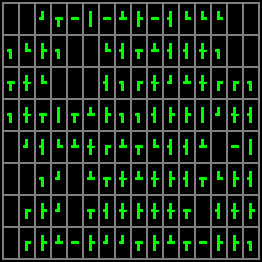
\includegraphics[scale=0.75]{\CURPATH/shuffled.png}
\caption{Разобранная головоломка}
\end{figure}

\dots и собранная:

\begin{figure}[H]
\label{fig:pipe_solved}
\centering
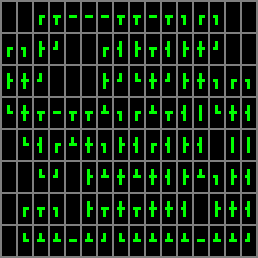
\includegraphics[scale=0.75]{\CURPATH/solved.png}
\caption{Собранная головоломка}
\end{figure}

Попробуем найти способ собрать её.

\subsubsection{Создание}

В начале, нужно её создать.
Вот простая идея.
Возьем массив ячеек 8*16.
Каждая ячейка может содержать какой-то тип блока.
Между ячейками есть стыки:

\input{\CURPATH/pipe_gen.tex}

Синие линии это горизонтальные стыки, красные линии это вертикальные стыки.
Мы просто случайно выставляем каждый стык в 0/false (отсутствует) или 1/true (присутствует).

После этого, теперь легко найти тип каждой ячейки.
А это:

\newcommand{\HeaderColor}{\cellcolor{blue!25}}
\begin{center}
\begin{longtable}{ | l | l | l | l | }
\hline
\HeaderColor стыки & \HeaderColor наше внутреннее название & \HeaderColor угол & \HeaderColor символ \\
\hline
0	&type 0		&	0$^{\circ}$	& (пробел)	\\
2	&type 2a	&	0$^{\circ}$	& \pmboxdrawuni{2503} \\ % ┃
2	&type 2a	&	90$^{\circ}$	& \pmboxdrawuni{2501} \\ % ━
2	&type 2b	&	0$^{\circ}$	& \pmboxdrawuni{250F} \\ % ┏
2	&type 2b	&	90$^{\circ}$	& \pmboxdrawuni{2513} \\ % ┓
2	&type 2b	&	180$^{\circ}$	& \pmboxdrawuni{251B} \\ % ┛
2	&type 2b	&	270$^{\circ}$	& \pmboxdrawuni{2517} \\ % ┗
3	&type 3		&	0$^{\circ}$	& \pmboxdrawuni{2523} \\ % ┣
3 	&type 3		&	90$^{\circ}$	& \pmboxdrawuni{2533} \\ % ┳
3	&type 3		&	180$^{\circ}$	& \pmboxdrawuni{252B} \\ % ┫
3	&type 3		&	270$^{\circ}$	& \pmboxdrawuni{253B} \\ % ┻
4	&type 4		&	0$^{\circ}$	& \pmboxdrawuni{254B} \\ % ╋
\hline
\end{longtable}
\end{center}

\textit{Висящие} стыки могут присутствовать на первой стадии (т.е., ячейки только с одним стыком), но они удалются
рекурсивно, и эти ячейки преобразуются в пустые ячейки.
Так что, в самом конце, все ячейки имеют минимум 2 стыка, и вся эта сантехническая система не имеет связей с внешним миром ---
я надеюсь, из-за этого станет немного проще.

Исходник генератора на Си здесь: \url{.../pipe/generator}.
Все вертикальные стыки хранятся в глобальном массиве \textit{hjoints[]} и вертикальные в \textit{vjoints[]}.

Программа на Си генерирует ANSI-раскрашенный вывод, как это было показано выше
(\ref{fig:pipe_shuffled}, \ref{fig:pipe_solved}) плюс массив типов для каждой ячейки, но без информации об углах:

\begin{lstlisting}[label=init_cells]
[
["0", "0", "2b", "3", "2a", "2a", "2a", "3", "3", "2a", "3", "2b", "2b", "2b", "0", "0"],
["2b", "2b", "3", "2b", "0", "0", "2b", "3", "3", "3", "3", "3", "4", "2b", "0", "0"],
["3", "4", "2b", "0", "0", "0", "3", "2b", "2b", "4", "2b", "3", "4", "2b", "2b", "2b"],
["2b", "4", "3", "2a", "3", "3", "3", "2b", "2b", "3", "3", "3", "2a", "2b", "4", "3"],
["0", "2b", "3", "2b", "3", "4", "2b", "3", "3", "2b", "3", "3", "3", "0", "2a", "2a"],
["0", "0", "2b", "2b", "0", "3", "3", "4", "3", "4", "3", "3", "3", "2b", "3", "3"],
["0", "2b", "3", "2b", "0", "3", "3", "4", "3", "4", "4", "3", "0", "3", "4", "3"],
["0", "2b", "3", "3", "2a", "3", "2b", "2b", "3", "3", "3", "3", "2a", "3", "3", "2b"],
]
\end{lstlisting}

\subsubsection{Решение}

Прежде всего, мы будем работать с массивом ячеек 8*16, где каждый элемент имеет 4 бита:
``T'' (top/верх),
``B'' (bottom/низ),
``L'' (left/лево),
``R'' (right/право).
Каждый бит представляет собой половину стыка.

\input{\CURPATH/pipe_solve.tex}

Теперь определяем массив для каждого из четырех полустыков + информация об угле:

\begin{lstlisting}
HEIGHT=8
WIDTH=16

# if T/B/R/L is Bool instead of Int, Z3 solver will work faster
T=[[Bool('cell_%d_%d_top' % (r, c)) for c in range(WIDTH)] for r in range(HEIGHT)]
B=[[Bool('cell_%d_%d_bottom' % (r, c)) for c in range(WIDTH)] for r in range(HEIGHT)]
R=[[Bool('cell_%d_%d_right' % (r, c)) for c in range(WIDTH)] for r in range(HEIGHT)]
L=[[Bool('cell_%d_%d_left' % (r, c)) for c in range(WIDTH)] for r in range(HEIGHT)]
A=[[Int('cell_%d_%d_angle' % (r, c)) for c in range(WIDTH)] for r in range(HEIGHT)]
\end{lstlisting}

Мы знаем, что если каждый из полустыков присутствует, ответный полустык также должен присутствовать, и наоборот. 
Определяем всё это используя эти констрайнты:

\begin{lstlisting}
# shorthand variables for True and False:
t=True
f=False

# "top" of each cell must be equal to "bottom" of the cell above
# "bottom" of each cell must be equal to "top" of the cell below
# "left" of each cell must be equal to "right" of the cell at left
# "right" of each cell must be equal to "left" of the cell at right
for r in range(HEIGHT):
    for c in range(WIDTH):
        if r!=0:
            s.add(T[r][c]==B[r-1][c])
        if r!=HEIGHT-1:
            s.add(B[r][c]==T[r+1][c])
        if c!=0:
            s.add(L[r][c]==R[r][c-1])
        if c!=WIDTH-1:
            s.add(R[r][c]==L[r][c+1])

# "left" of each cell of first column shouldn't have any connection
# so is "right" of each cell of the last column
for r in range(HEIGHT):
    s.add(L[r][0]==f)
    s.add(R[r][WIDTH-1]==f)

# "top" of each cell of the first row shouldn't have any connection
# so is "bottom" of each cell of the last row
for c in range(WIDTH):
    s.add(T[0][c]==f)
    s.add(B[HEIGHT-1][c]==f)
\end{lstlisting}

Теперь перебираем все ячейки в изначальном массиве (\ref{init_cells}).
Первые две ячейки здесь пустые. И третья имеет тип ``2b''.
Это ``\pmboxdrawuni{250F}'' % ┏
и его можно ориентировать четырьмя разными способами.
И если её угол это 0$^{\circ}$, верхний и правый полустыки присутствуют, остальные отсутствуют.
Если он имеет угол 90$^{\circ}$, он выглядит как 
``\pmboxdrawuni{2513}'', % ┓
и верхник и левый полустыки присутствуют, остальные отсутствуют.

На обычном русском языке: ``если ячейка этого типа имеет угол 0$^{\circ}$, вот эти полустыки должны присутствовать \textbf{ИЛИ}
если она имеет угол 90$^{\circ}$, эти полустыки должны присутствовать, \textbf{ИЛИ}, итд, итд.''

Точно также, мы определяем эти правила для всех типов и всех возможных углов:

\begin{lstlisting}
for r in range(HEIGHT):
    for c in range(WIDTH):
        ty=cells_type[r][c]

        if ty=="0":
            s.add(A[r][c]==f)
            s.add(T[r][c]==f, B[r][c]==f, L[r][c]==f, R[r][c]==f)

        if ty=="2a":
            s.add(Or(And(A[r][c]==0, L[r][c]==f, R[r][c]==f, T[r][c]==t, B[r][c]==t),   # §\pmboxdrawuni{2503}§
                    And(A[r][c]==90, L[r][c]==t, R[r][c]==t, T[r][c]==f, B[r][c]==f)))  # §\pmboxdrawuni{2501}§

        if ty=="2b":
            s.add(Or(And(A[r][c]==0, L[r][c]==f, R[r][c]==t, T[r][c]==f, B[r][c]==t),   # §\pmboxdrawuni{250F}§
                    And(A[r][c]==90, L[r][c]==t, R[r][c]==f, T[r][c]==f, B[r][c]==t),   # §\pmboxdrawuni{2513}§
                    And(A[r][c]==180, L[r][c]==t, R[r][c]==f, T[r][c]==t, B[r][c]==f),  # §\pmboxdrawuni{251B}§
                    And(A[r][c]==270, L[r][c]==f, R[r][c]==t, T[r][c]==t, B[r][c]==f))) # §\pmboxdrawuni{2517}§
	
        if ty=="3":
            s.add(Or(And(A[r][c]==0, L[r][c]==f, R[r][c]==t, T[r][c]==t, B[r][c]==t),   # §\pmboxdrawuni{2523}§
                    And(A[r][c]==90, L[r][c]==t, R[r][c]==t, T[r][c]==f, B[r][c]==t),   # §\pmboxdrawuni{2533}§
                    And(A[r][c]==180, L[r][c]==t, R[r][c]==f, T[r][c]==t, B[r][c]==t),  # §\pmboxdrawuni{252B}§
                    And(A[r][c]==270, L[r][c]==t, R[r][c]==t, T[r][c]==t, B[r][c]==f))) # §\pmboxdrawuni{253B}§

        if ty=="4":
            s.add(A[r][c]==0)
            s.add(T[r][c]==t, B[r][c]==t, L[r][c]==t, R[r][c]==t) # §\pmboxdrawuni{254B}§
\end{lstlisting}

Полный исходник здесь: \url{.../solver/solve_pipe_puzzle1.py}.

Получается такой результат (выводит угол для каждой ячейки и (псевдо)графическое представление):

\begin{figure}[H]
\centering
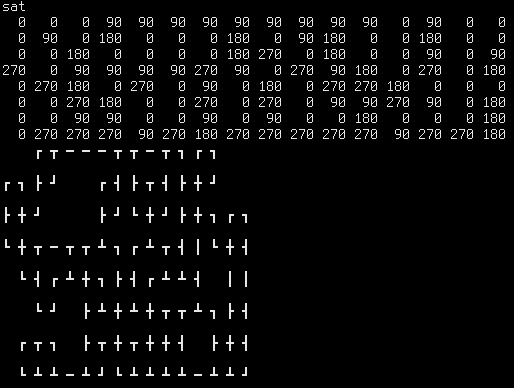
\includegraphics[scale=0.75]{\CURPATH/solver/solver.png}
\caption{Вывод скрипта солвера}
\end{figure}

Это работает $\approx 4$ секунды на моем старом и медленном Intel Atom N455 1.66GHz.
Быстро ли это? Не знаю, но снова вот что действительно круто, это то что мы понятия не имеем о какой-то математической
теории за всем этим, мы просто объявили ячейки, (полу-)стыки и определили отношения между ними.

Теперь следующий вопрос это, сколько здесь возможных решений?
Используя раннее описанный метод (\ref{SMTEnumerate}), я немного изменил скрипт солвера
\footnote{\url{.../solver/solve_pipe_puzzle2.py}} и солвер
сказал что возможно два решения.

Сравним их используя gvimdiff:

\begin{figure}[H]
\centering
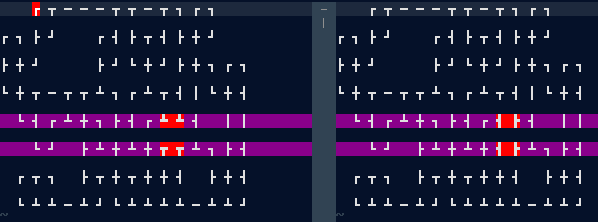
\includegraphics[scale=0.75]{\CURPATH/solver/diff.png}
\caption{Вывод gvimdiff (извините за мой красный курсор в левой части в левом верхнем углу)}
\end{figure}

4 ячейки в середине могут быть ориентированы по-разному.
Видимо, другие головоломки могут также выдавать разные результаты.

P.S.
\textit{Полу-стык} определен как булевый тип.
Но на самом деле, первая версия солвера была написана используя целочисленный тип для полу-стыков,
и 0 использовалось для False и 1 для True.
Я так сделал, потому что хотел более компактный исходный код, без использования длинных слов как ``False'' и ``True''.
И это работало, но медленнее. Вероятно, Z3 работает с булевыми типами быстрее? Лучше?
Так или иначе, я пишу это чтобы отметить, что, если нужно, целочисленный тип можно использовать вместо булевого.


\section{Развлекательная математика и головоломки}

\input{puzzles/sudoku/main_RU}
\input{puzzles/zebra/main_RU}
\input{puzzles/pipe/main_RU}
\input{puzzles/rubik2/failed_SMT/main_RU}
\input{puzzles/rubik2/SAT/main_RU}
\input{puzzles/rubik3/one_face_SMT/main_RU}
%\input{puzzles/numberlink/main_RU}
%\input{puzzles/two_parks_RU}
\input{puzzles/alphametics/main_RU}
%\input{puzzles/2015_AIME_II_Problems_12_RU}
%\input{puzzles/fred/main_RU}
%\input{puzzles/MC/main_RU}
%\input{puzzles/coin_flip/main_RU}
%\input{puzzles/Mock_AIME_2_2006-2007_Problem_8_RU}
%\input{puzzles/2012_AIME_I_Problems_1_RU}
%\input{puzzles/keypad_RU}


\section{Развлекательная математика и головоломки}

\input{puzzles/sudoku/main_RU}
\input{puzzles/zebra/main_RU}
\input{puzzles/pipe/main_RU}
\input{puzzles/rubik2/failed_SMT/main_RU}
\input{puzzles/rubik2/SAT/main_RU}
\input{puzzles/rubik3/one_face_SMT/main_RU}
%\input{puzzles/numberlink/main_RU}
%\input{puzzles/two_parks_RU}
\input{puzzles/alphametics/main_RU}
%\input{puzzles/2015_AIME_II_Problems_12_RU}
%\input{puzzles/fred/main_RU}
%\input{puzzles/MC/main_RU}
%\input{puzzles/coin_flip/main_RU}
%\input{puzzles/Mock_AIME_2_2006-2007_Problem_8_RU}
%\input{puzzles/2012_AIME_I_Problems_1_RU}
%\input{puzzles/keypad_RU}


\section{Развлекательная математика и головоломки}

\input{puzzles/sudoku/main_RU}
\input{puzzles/zebra/main_RU}
\input{puzzles/pipe/main_RU}
\input{puzzles/rubik2/failed_SMT/main_RU}
\input{puzzles/rubik2/SAT/main_RU}
\input{puzzles/rubik3/one_face_SMT/main_RU}
%\input{puzzles/numberlink/main_RU}
%\input{puzzles/two_parks_RU}
\input{puzzles/alphametics/main_RU}
%\input{puzzles/2015_AIME_II_Problems_12_RU}
%\input{puzzles/fred/main_RU}
%\input{puzzles/MC/main_RU}
%\input{puzzles/coin_flip/main_RU}
%\input{puzzles/Mock_AIME_2_2006-2007_Problem_8_RU}
%\input{puzzles/2012_AIME_I_Problems_1_RU}
%\input{puzzles/keypad_RU}


%\section{Развлекательная математика и головоломки}

\input{puzzles/sudoku/main_RU}
\input{puzzles/zebra/main_RU}
\input{puzzles/pipe/main_RU}
\input{puzzles/rubik2/failed_SMT/main_RU}
\input{puzzles/rubik2/SAT/main_RU}
\input{puzzles/rubik3/one_face_SMT/main_RU}
%\input{puzzles/numberlink/main_RU}
%\input{puzzles/two_parks_RU}
\input{puzzles/alphametics/main_RU}
%\input{puzzles/2015_AIME_II_Problems_12_RU}
%\input{puzzles/fred/main_RU}
%\input{puzzles/MC/main_RU}
%\input{puzzles/coin_flip/main_RU}
%\input{puzzles/Mock_AIME_2_2006-2007_Problem_8_RU}
%\input{puzzles/2012_AIME_I_Problems_1_RU}
%\input{puzzles/keypad_RU}


%\input{puzzles/two_parks_RU}
\subsection{Альфаметика}

Согласно Дональду Кнуту, термин ``Альфаметика'' был придуман Дж. Эйч. Аш. Хантером.
Это головоломка: какие десятичные цифры в пределах 0..9 нужно присвоить каждой букве, чтобы это уравнение было справедливо?

\begin{lstlisting}
  SEND
+ MORE
 -----
 MONEY
\end{lstlisting}

Для Z3 это легко:

\lstinputlisting{puzzles/alphametics/alpha.py}

Вывод:

\begin{lstlisting}
sat
[E, = 5,
 S, = 9,
 M, = 1,
 N, = 6,
 D, = 7,
 R, = 8,
 O, = 0,
 Y = 2]
\end{lstlisting}

Вот еще одна, из \ac{TAOCP} том IV (\url{http://www-cs-faculty.stanford.edu/~uno/fasc2b.ps.gz}):

\lstinputlisting{puzzles/alphametics/alpha2.py}

\begin{lstlisting}
sat
[L, = 6,
 S, = 7,
 N, = 2,
 T, = 1,
 I, = 5,
 V = 3,
 A, = 8,
 R, = 9,
 O, = 4,
 TRIO = 1954,
 SONATA, = 742818,
 VIOLA, = 35468,
 VIOLIN, = 354652]
\end{lstlisting}

% TODO URL
Эту головоломку я нашел в примерах pySMT:

\lstinputlisting{puzzles/alphametics/alpha3.py}

\begin{lstlisting}
sat
[D = 5, R = 4, O = 3, E = 8, L = 6, W = 7, H = 2]
\end{lstlisting}

%%% 

Это упражнение Q209 из
[Companion to the Papers of Donald Knuth]\footnote{\url{http://www-cs-faculty.stanford.edu/~knuth/cp.html}}.

\begin{lstlisting}
 KNIFE
  FORK
 SPOON
  SOUP
------
SUPPER
\end{lstlisting}

В целях упрощения, я добавил ф-цию (list\_to\_expr()):

\lstinputlisting{puzzles/alphametics/alpha4.py}

\begin{lstlisting}
sat
[K = 7,
 N = 4,
 R = 9,
 I = 1,
 E = 6,
 S = 0,
 O = 3,
 F = 5,
 U = 8,
 P = 2,
 SUPPER = 82269,
 SOUP = 382,
 SPOON = 2334,
 FORK = 5397,
 KNIFE = 74156]
\end{lstlisting}

S это 0, так что значение SUPPER начинается с (убранного) нуля. Скажем так, нам это не нравится.
Добавим это, чтобы это исправить:

\begin{lstlisting}
s.add(S!=0)
\end{lstlisting}

\begin{lstlisting}
sat
[K = 8,
 N = 4,
 R = 3,
 I = 7,
 E = 6,
 S = 1,
 O = 9,
 F = 2,
 U = 0,
 P = 5,
 SUPPER = 105563,
 SOUP = 1905,
 SPOON = 15994,
 FORK = 2938,
 KNIFE = 84726]
\end{lstlisting}

\paragraph{Создание своей собственной головоломки}

Вот проблема: есть только 10 букв, но как их выбрать из числа слов?
Мы можем использовать Z3 для этого:

\lstinputlisting{puzzles/alphametics/gen.py}

Это первая сгенерированная головоломка:

\begin{lstlisting}
sat
EGGS
JELLY
LUNCH
C 5
E 6
G 3
H 7
J 0
L 1
N 4
S 8
U 2
Y 9
\end{lstlisting}

Что если мы хотим, чтобы слово ``CAKE'' присутствовало в числе ``слагаемых''?

Добавим это:

\begin{lstlisting}
s.add(word_used[words.index('CAKE')])
\end{lstlisting}

\begin{lstlisting}
sat
CAKE
TEA
LUNCH
A 8
C 3
E 1
H 9
J 6
K 2
L 0
N 5
T 7
U 4
\end{lstlisting}

Добавим это:

\begin{lstlisting}
s.add(word_used[words.index('EGGS')])
\end{lstlisting}

Теперь оно может найти пару к EGGS:

\begin{lstlisting}
sat
EGGS
HONEY
LUNCH
C 6
E 7
G 9
H 4
L 5
N 8
O 2
S 3
U 0
Y 1
\end{lstlisting}

\paragraph{Файлы}

\url{https://github.com/DennisYurichev/...}




%\input{puzzles/2015_AIME_II_Problems_12_RU}
%\section{Развлекательная математика и головоломки}

\input{puzzles/sudoku/main_RU}
\input{puzzles/zebra/main_RU}
\input{puzzles/pipe/main_RU}
\input{puzzles/rubik2/failed_SMT/main_RU}
\input{puzzles/rubik2/SAT/main_RU}
\input{puzzles/rubik3/one_face_SMT/main_RU}
%\input{puzzles/numberlink/main_RU}
%\input{puzzles/two_parks_RU}
\input{puzzles/alphametics/main_RU}
%\input{puzzles/2015_AIME_II_Problems_12_RU}
%\input{puzzles/fred/main_RU}
%\input{puzzles/MC/main_RU}
%\input{puzzles/coin_flip/main_RU}
%\input{puzzles/Mock_AIME_2_2006-2007_Problem_8_RU}
%\input{puzzles/2012_AIME_I_Problems_1_RU}
%\input{puzzles/keypad_RU}


%\section{Развлекательная математика и головоломки}

\input{puzzles/sudoku/main_RU}
\input{puzzles/zebra/main_RU}
\input{puzzles/pipe/main_RU}
\input{puzzles/rubik2/failed_SMT/main_RU}
\input{puzzles/rubik2/SAT/main_RU}
\input{puzzles/rubik3/one_face_SMT/main_RU}
%\input{puzzles/numberlink/main_RU}
%\input{puzzles/two_parks_RU}
\input{puzzles/alphametics/main_RU}
%\input{puzzles/2015_AIME_II_Problems_12_RU}
%\input{puzzles/fred/main_RU}
%\input{puzzles/MC/main_RU}
%\input{puzzles/coin_flip/main_RU}
%\input{puzzles/Mock_AIME_2_2006-2007_Problem_8_RU}
%\input{puzzles/2012_AIME_I_Problems_1_RU}
%\input{puzzles/keypad_RU}


%\section{Развлекательная математика и головоломки}

\input{puzzles/sudoku/main_RU}
\input{puzzles/zebra/main_RU}
\input{puzzles/pipe/main_RU}
\input{puzzles/rubik2/failed_SMT/main_RU}
\input{puzzles/rubik2/SAT/main_RU}
\input{puzzles/rubik3/one_face_SMT/main_RU}
%\input{puzzles/numberlink/main_RU}
%\input{puzzles/two_parks_RU}
\input{puzzles/alphametics/main_RU}
%\input{puzzles/2015_AIME_II_Problems_12_RU}
%\input{puzzles/fred/main_RU}
%\input{puzzles/MC/main_RU}
%\input{puzzles/coin_flip/main_RU}
%\input{puzzles/Mock_AIME_2_2006-2007_Problem_8_RU}
%\input{puzzles/2012_AIME_I_Problems_1_RU}
%\input{puzzles/keypad_RU}


%\input{puzzles/Mock_AIME_2_2006-2007_Problem_8_RU}
%\input{puzzles/2012_AIME_I_Problems_1_RU}
%\input{puzzles/keypad_RU}


%\section{Развлекательная математика и головоломки}

\subsection{Судоку}

Головоломка Судоку это решетка 9*9, некоторые ячейки заполнены значениями, некоторые пустые:

% copypasted from http://www.texample.net/tikz/examples/sudoku/
\newcounter{row}
\newcounter{col}

\newcommand\setrow[9]{
  \setcounter{col}{1}
  \foreach \n in {#1, #2, #3, #4, #5, #6, #7, #8, #9} {
    \edef\x{\value{col} - 0.5}
    \edef\y{9.5 - \value{row}}
    \node[anchor=center] at (\x, \y) {\n};
    \stepcounter{col}
  }
  \stepcounter{row}
}

\begin{center}
\begin{tikzpicture}[scale=.7]
  \begin{scope}
    \draw (0, 0) grid (9, 9);
    \draw[very thick, scale=3] (0, 0) grid (3, 3);

    \setcounter{row}{1}
    \setrow { }{ }{5}  {3}{ }{ }  { }{ }{ }
    \setrow {8}{ }{ }  { }{ }{ }  { }{2}{ }
    \setrow { }{7}{ }  { }{1}{ }  {5}{ }{ }

    \setrow {4}{ }{ }  { }{ }{5}  {3}{ }{ }
    \setrow { }{1}{ }  { }{7}{ }  { }{ }{6}
    \setrow { }{ }{3}  {2}{ }{ }  { }{8}{ }

    \setrow { }{6}{ }  {5}{ }{ }  { }{ }{9}
    \setrow { }{ }{4}  { }{ }{ }  { }{3}{ }
    \setrow { }{ }{ }  { }{ }{9}  {7}{ }{ }

    \node[anchor=center] at (4.5, -0.5) {Нерешенная Судоку};
  \end{scope}
\end{tikzpicture}
\end{center}

Числа в каждом ряду должны быть уникальными, т.е., каждый ряд должен содержать 9 чисел в пределах 1..9 без повторений.
Та же история и для каждого столбца и каждого квадрата 3*3.

Головоломка представляет собой хороший кандидат, на котором можно попробовать \ac{SMT}-солвер, потому что это,
в общем-то, просто нерешенная система уравнений.

\input{puzzles/sudoku/1/main_RU}
%\input{puzzles/sudoku/GT/main_RU}
%\input{puzzles/sudoku/killer/main_RU}
\input{puzzles/sudoku/KLEE/main_RU}
\input{puzzles/sudoku/SAT/main_RU}


\subsection{Головоломка зебры (\ac{AKA} Загадка Эйнштейна)}

\input{puzzles/zebra/SMT/main_RU}
\input{puzzles/zebra/KLEE/main_RU}
\input{puzzles/zebra/SAT/main_RU}


\subsection{Решение головоломки ``трубы'' используя Z3 SMT-солвер}

\renewcommand{\CURPATH}{puzzles/pipe}

Головоломка ``трубы'' это популярная головоломка (просто погуглите ``pipe puzzle'' и посмотрите на картинки).

Вот как выглядит головоломка в разобранном виде:

\begin{figure}[H]
\label{fig:pipe_shuffled}
\centering
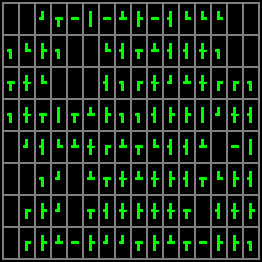
\includegraphics[scale=0.75]{\CURPATH/shuffled.png}
\caption{Разобранная головоломка}
\end{figure}

\dots и собранная:

\begin{figure}[H]
\label{fig:pipe_solved}
\centering
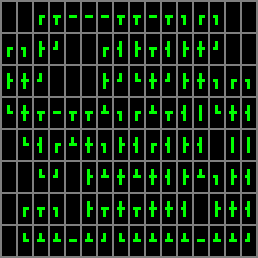
\includegraphics[scale=0.75]{\CURPATH/solved.png}
\caption{Собранная головоломка}
\end{figure}

Попробуем найти способ собрать её.

\subsubsection{Создание}

В начале, нужно её создать.
Вот простая идея.
Возьем массив ячеек 8*16.
Каждая ячейка может содержать какой-то тип блока.
Между ячейками есть стыки:

\input{\CURPATH/pipe_gen.tex}

Синие линии это горизонтальные стыки, красные линии это вертикальные стыки.
Мы просто случайно выставляем каждый стык в 0/false (отсутствует) или 1/true (присутствует).

После этого, теперь легко найти тип каждой ячейки.
А это:

\newcommand{\HeaderColor}{\cellcolor{blue!25}}
\begin{center}
\begin{longtable}{ | l | l | l | l | }
\hline
\HeaderColor стыки & \HeaderColor наше внутреннее название & \HeaderColor угол & \HeaderColor символ \\
\hline
0	&type 0		&	0$^{\circ}$	& (пробел)	\\
2	&type 2a	&	0$^{\circ}$	& \pmboxdrawuni{2503} \\ % ┃
2	&type 2a	&	90$^{\circ}$	& \pmboxdrawuni{2501} \\ % ━
2	&type 2b	&	0$^{\circ}$	& \pmboxdrawuni{250F} \\ % ┏
2	&type 2b	&	90$^{\circ}$	& \pmboxdrawuni{2513} \\ % ┓
2	&type 2b	&	180$^{\circ}$	& \pmboxdrawuni{251B} \\ % ┛
2	&type 2b	&	270$^{\circ}$	& \pmboxdrawuni{2517} \\ % ┗
3	&type 3		&	0$^{\circ}$	& \pmboxdrawuni{2523} \\ % ┣
3 	&type 3		&	90$^{\circ}$	& \pmboxdrawuni{2533} \\ % ┳
3	&type 3		&	180$^{\circ}$	& \pmboxdrawuni{252B} \\ % ┫
3	&type 3		&	270$^{\circ}$	& \pmboxdrawuni{253B} \\ % ┻
4	&type 4		&	0$^{\circ}$	& \pmboxdrawuni{254B} \\ % ╋
\hline
\end{longtable}
\end{center}

\textit{Висящие} стыки могут присутствовать на первой стадии (т.е., ячейки только с одним стыком), но они удалются
рекурсивно, и эти ячейки преобразуются в пустые ячейки.
Так что, в самом конце, все ячейки имеют минимум 2 стыка, и вся эта сантехническая система не имеет связей с внешним миром ---
я надеюсь, из-за этого станет немного проще.

Исходник генератора на Си здесь: \url{.../pipe/generator}.
Все вертикальные стыки хранятся в глобальном массиве \textit{hjoints[]} и вертикальные в \textit{vjoints[]}.

Программа на Си генерирует ANSI-раскрашенный вывод, как это было показано выше
(\ref{fig:pipe_shuffled}, \ref{fig:pipe_solved}) плюс массив типов для каждой ячейки, но без информации об углах:

\begin{lstlisting}[label=init_cells]
[
["0", "0", "2b", "3", "2a", "2a", "2a", "3", "3", "2a", "3", "2b", "2b", "2b", "0", "0"],
["2b", "2b", "3", "2b", "0", "0", "2b", "3", "3", "3", "3", "3", "4", "2b", "0", "0"],
["3", "4", "2b", "0", "0", "0", "3", "2b", "2b", "4", "2b", "3", "4", "2b", "2b", "2b"],
["2b", "4", "3", "2a", "3", "3", "3", "2b", "2b", "3", "3", "3", "2a", "2b", "4", "3"],
["0", "2b", "3", "2b", "3", "4", "2b", "3", "3", "2b", "3", "3", "3", "0", "2a", "2a"],
["0", "0", "2b", "2b", "0", "3", "3", "4", "3", "4", "3", "3", "3", "2b", "3", "3"],
["0", "2b", "3", "2b", "0", "3", "3", "4", "3", "4", "4", "3", "0", "3", "4", "3"],
["0", "2b", "3", "3", "2a", "3", "2b", "2b", "3", "3", "3", "3", "2a", "3", "3", "2b"],
]
\end{lstlisting}

\subsubsection{Решение}

Прежде всего, мы будем работать с массивом ячеек 8*16, где каждый элемент имеет 4 бита:
``T'' (top/верх),
``B'' (bottom/низ),
``L'' (left/лево),
``R'' (right/право).
Каждый бит представляет собой половину стыка.

\input{\CURPATH/pipe_solve.tex}

Теперь определяем массив для каждого из четырех полустыков + информация об угле:

\begin{lstlisting}
HEIGHT=8
WIDTH=16

# if T/B/R/L is Bool instead of Int, Z3 solver will work faster
T=[[Bool('cell_%d_%d_top' % (r, c)) for c in range(WIDTH)] for r in range(HEIGHT)]
B=[[Bool('cell_%d_%d_bottom' % (r, c)) for c in range(WIDTH)] for r in range(HEIGHT)]
R=[[Bool('cell_%d_%d_right' % (r, c)) for c in range(WIDTH)] for r in range(HEIGHT)]
L=[[Bool('cell_%d_%d_left' % (r, c)) for c in range(WIDTH)] for r in range(HEIGHT)]
A=[[Int('cell_%d_%d_angle' % (r, c)) for c in range(WIDTH)] for r in range(HEIGHT)]
\end{lstlisting}

Мы знаем, что если каждый из полустыков присутствует, ответный полустык также должен присутствовать, и наоборот. 
Определяем всё это используя эти констрайнты:

\begin{lstlisting}
# shorthand variables for True and False:
t=True
f=False

# "top" of each cell must be equal to "bottom" of the cell above
# "bottom" of each cell must be equal to "top" of the cell below
# "left" of each cell must be equal to "right" of the cell at left
# "right" of each cell must be equal to "left" of the cell at right
for r in range(HEIGHT):
    for c in range(WIDTH):
        if r!=0:
            s.add(T[r][c]==B[r-1][c])
        if r!=HEIGHT-1:
            s.add(B[r][c]==T[r+1][c])
        if c!=0:
            s.add(L[r][c]==R[r][c-1])
        if c!=WIDTH-1:
            s.add(R[r][c]==L[r][c+1])

# "left" of each cell of first column shouldn't have any connection
# so is "right" of each cell of the last column
for r in range(HEIGHT):
    s.add(L[r][0]==f)
    s.add(R[r][WIDTH-1]==f)

# "top" of each cell of the first row shouldn't have any connection
# so is "bottom" of each cell of the last row
for c in range(WIDTH):
    s.add(T[0][c]==f)
    s.add(B[HEIGHT-1][c]==f)
\end{lstlisting}

Теперь перебираем все ячейки в изначальном массиве (\ref{init_cells}).
Первые две ячейки здесь пустые. И третья имеет тип ``2b''.
Это ``\pmboxdrawuni{250F}'' % ┏
и его можно ориентировать четырьмя разными способами.
И если её угол это 0$^{\circ}$, верхний и правый полустыки присутствуют, остальные отсутствуют.
Если он имеет угол 90$^{\circ}$, он выглядит как 
``\pmboxdrawuni{2513}'', % ┓
и верхник и левый полустыки присутствуют, остальные отсутствуют.

На обычном русском языке: ``если ячейка этого типа имеет угол 0$^{\circ}$, вот эти полустыки должны присутствовать \textbf{ИЛИ}
если она имеет угол 90$^{\circ}$, эти полустыки должны присутствовать, \textbf{ИЛИ}, итд, итд.''

Точно также, мы определяем эти правила для всех типов и всех возможных углов:

\begin{lstlisting}
for r in range(HEIGHT):
    for c in range(WIDTH):
        ty=cells_type[r][c]

        if ty=="0":
            s.add(A[r][c]==f)
            s.add(T[r][c]==f, B[r][c]==f, L[r][c]==f, R[r][c]==f)

        if ty=="2a":
            s.add(Or(And(A[r][c]==0, L[r][c]==f, R[r][c]==f, T[r][c]==t, B[r][c]==t),   # §\pmboxdrawuni{2503}§
                    And(A[r][c]==90, L[r][c]==t, R[r][c]==t, T[r][c]==f, B[r][c]==f)))  # §\pmboxdrawuni{2501}§

        if ty=="2b":
            s.add(Or(And(A[r][c]==0, L[r][c]==f, R[r][c]==t, T[r][c]==f, B[r][c]==t),   # §\pmboxdrawuni{250F}§
                    And(A[r][c]==90, L[r][c]==t, R[r][c]==f, T[r][c]==f, B[r][c]==t),   # §\pmboxdrawuni{2513}§
                    And(A[r][c]==180, L[r][c]==t, R[r][c]==f, T[r][c]==t, B[r][c]==f),  # §\pmboxdrawuni{251B}§
                    And(A[r][c]==270, L[r][c]==f, R[r][c]==t, T[r][c]==t, B[r][c]==f))) # §\pmboxdrawuni{2517}§
	
        if ty=="3":
            s.add(Or(And(A[r][c]==0, L[r][c]==f, R[r][c]==t, T[r][c]==t, B[r][c]==t),   # §\pmboxdrawuni{2523}§
                    And(A[r][c]==90, L[r][c]==t, R[r][c]==t, T[r][c]==f, B[r][c]==t),   # §\pmboxdrawuni{2533}§
                    And(A[r][c]==180, L[r][c]==t, R[r][c]==f, T[r][c]==t, B[r][c]==t),  # §\pmboxdrawuni{252B}§
                    And(A[r][c]==270, L[r][c]==t, R[r][c]==t, T[r][c]==t, B[r][c]==f))) # §\pmboxdrawuni{253B}§

        if ty=="4":
            s.add(A[r][c]==0)
            s.add(T[r][c]==t, B[r][c]==t, L[r][c]==t, R[r][c]==t) # §\pmboxdrawuni{254B}§
\end{lstlisting}

Полный исходник здесь: \url{.../solver/solve_pipe_puzzle1.py}.

Получается такой результат (выводит угол для каждой ячейки и (псевдо)графическое представление):

\begin{figure}[H]
\centering
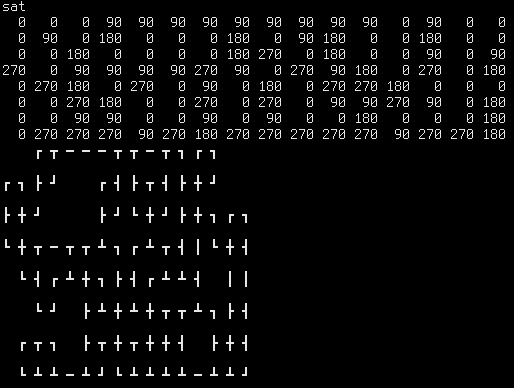
\includegraphics[scale=0.75]{\CURPATH/solver/solver.png}
\caption{Вывод скрипта солвера}
\end{figure}

Это работает $\approx 4$ секунды на моем старом и медленном Intel Atom N455 1.66GHz.
Быстро ли это? Не знаю, но снова вот что действительно круто, это то что мы понятия не имеем о какой-то математической
теории за всем этим, мы просто объявили ячейки, (полу-)стыки и определили отношения между ними.

Теперь следующий вопрос это, сколько здесь возможных решений?
Используя раннее описанный метод (\ref{SMTEnumerate}), я немного изменил скрипт солвера
\footnote{\url{.../solver/solve_pipe_puzzle2.py}} и солвер
сказал что возможно два решения.

Сравним их используя gvimdiff:

\begin{figure}[H]
\centering
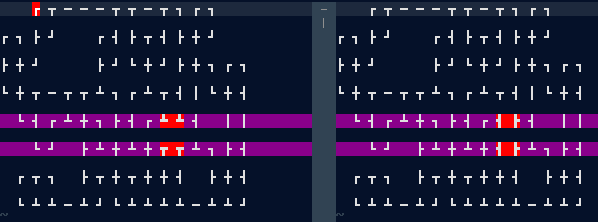
\includegraphics[scale=0.75]{\CURPATH/solver/diff.png}
\caption{Вывод gvimdiff (извините за мой красный курсор в левой части в левом верхнем углу)}
\end{figure}

4 ячейки в середине могут быть ориентированы по-разному.
Видимо, другие головоломки могут также выдавать разные результаты.

P.S.
\textit{Полу-стык} определен как булевый тип.
Но на самом деле, первая версия солвера была написана используя целочисленный тип для полу-стыков,
и 0 использовалось для False и 1 для True.
Я так сделал, потому что хотел более компактный исходный код, без использования длинных слов как ``False'' и ``True''.
И это работало, но медленнее. Вероятно, Z3 работает с булевыми типами быстрее? Лучше?
Так или иначе, я пишу это чтобы отметить, что, если нужно, целочисленный тип можно использовать вместо булевого.


\section{Развлекательная математика и головоломки}

\input{puzzles/sudoku/main_RU}
\input{puzzles/zebra/main_RU}
\input{puzzles/pipe/main_RU}
\input{puzzles/rubik2/failed_SMT/main_RU}
\input{puzzles/rubik2/SAT/main_RU}
\input{puzzles/rubik3/one_face_SMT/main_RU}
%\input{puzzles/numberlink/main_RU}
%\input{puzzles/two_parks_RU}
\input{puzzles/alphametics/main_RU}
%\input{puzzles/2015_AIME_II_Problems_12_RU}
%\input{puzzles/fred/main_RU}
%\input{puzzles/MC/main_RU}
%\input{puzzles/coin_flip/main_RU}
%\input{puzzles/Mock_AIME_2_2006-2007_Problem_8_RU}
%\input{puzzles/2012_AIME_I_Problems_1_RU}
%\input{puzzles/keypad_RU}


\section{Развлекательная математика и головоломки}

\input{puzzles/sudoku/main_RU}
\input{puzzles/zebra/main_RU}
\input{puzzles/pipe/main_RU}
\input{puzzles/rubik2/failed_SMT/main_RU}
\input{puzzles/rubik2/SAT/main_RU}
\input{puzzles/rubik3/one_face_SMT/main_RU}
%\input{puzzles/numberlink/main_RU}
%\input{puzzles/two_parks_RU}
\input{puzzles/alphametics/main_RU}
%\input{puzzles/2015_AIME_II_Problems_12_RU}
%\input{puzzles/fred/main_RU}
%\input{puzzles/MC/main_RU}
%\input{puzzles/coin_flip/main_RU}
%\input{puzzles/Mock_AIME_2_2006-2007_Problem_8_RU}
%\input{puzzles/2012_AIME_I_Problems_1_RU}
%\input{puzzles/keypad_RU}


\section{Развлекательная математика и головоломки}

\input{puzzles/sudoku/main_RU}
\input{puzzles/zebra/main_RU}
\input{puzzles/pipe/main_RU}
\input{puzzles/rubik2/failed_SMT/main_RU}
\input{puzzles/rubik2/SAT/main_RU}
\input{puzzles/rubik3/one_face_SMT/main_RU}
%\input{puzzles/numberlink/main_RU}
%\input{puzzles/two_parks_RU}
\input{puzzles/alphametics/main_RU}
%\input{puzzles/2015_AIME_II_Problems_12_RU}
%\input{puzzles/fred/main_RU}
%\input{puzzles/MC/main_RU}
%\input{puzzles/coin_flip/main_RU}
%\input{puzzles/Mock_AIME_2_2006-2007_Problem_8_RU}
%\input{puzzles/2012_AIME_I_Problems_1_RU}
%\input{puzzles/keypad_RU}


%\section{Развлекательная математика и головоломки}

\input{puzzles/sudoku/main_RU}
\input{puzzles/zebra/main_RU}
\input{puzzles/pipe/main_RU}
\input{puzzles/rubik2/failed_SMT/main_RU}
\input{puzzles/rubik2/SAT/main_RU}
\input{puzzles/rubik3/one_face_SMT/main_RU}
%\input{puzzles/numberlink/main_RU}
%\input{puzzles/two_parks_RU}
\input{puzzles/alphametics/main_RU}
%\input{puzzles/2015_AIME_II_Problems_12_RU}
%\input{puzzles/fred/main_RU}
%\input{puzzles/MC/main_RU}
%\input{puzzles/coin_flip/main_RU}
%\input{puzzles/Mock_AIME_2_2006-2007_Problem_8_RU}
%\input{puzzles/2012_AIME_I_Problems_1_RU}
%\input{puzzles/keypad_RU}


%\input{puzzles/two_parks_RU}
\subsection{Альфаметика}

Согласно Дональду Кнуту, термин ``Альфаметика'' был придуман Дж. Эйч. Аш. Хантером.
Это головоломка: какие десятичные цифры в пределах 0..9 нужно присвоить каждой букве, чтобы это уравнение было справедливо?

\begin{lstlisting}
  SEND
+ MORE
 -----
 MONEY
\end{lstlisting}

Для Z3 это легко:

\lstinputlisting{puzzles/alphametics/alpha.py}

Вывод:

\begin{lstlisting}
sat
[E, = 5,
 S, = 9,
 M, = 1,
 N, = 6,
 D, = 7,
 R, = 8,
 O, = 0,
 Y = 2]
\end{lstlisting}

Вот еще одна, из \ac{TAOCP} том IV (\url{http://www-cs-faculty.stanford.edu/~uno/fasc2b.ps.gz}):

\lstinputlisting{puzzles/alphametics/alpha2.py}

\begin{lstlisting}
sat
[L, = 6,
 S, = 7,
 N, = 2,
 T, = 1,
 I, = 5,
 V = 3,
 A, = 8,
 R, = 9,
 O, = 4,
 TRIO = 1954,
 SONATA, = 742818,
 VIOLA, = 35468,
 VIOLIN, = 354652]
\end{lstlisting}

% TODO URL
Эту головоломку я нашел в примерах pySMT:

\lstinputlisting{puzzles/alphametics/alpha3.py}

\begin{lstlisting}
sat
[D = 5, R = 4, O = 3, E = 8, L = 6, W = 7, H = 2]
\end{lstlisting}

%%% 

Это упражнение Q209 из
[Companion to the Papers of Donald Knuth]\footnote{\url{http://www-cs-faculty.stanford.edu/~knuth/cp.html}}.

\begin{lstlisting}
 KNIFE
  FORK
 SPOON
  SOUP
------
SUPPER
\end{lstlisting}

В целях упрощения, я добавил ф-цию (list\_to\_expr()):

\lstinputlisting{puzzles/alphametics/alpha4.py}

\begin{lstlisting}
sat
[K = 7,
 N = 4,
 R = 9,
 I = 1,
 E = 6,
 S = 0,
 O = 3,
 F = 5,
 U = 8,
 P = 2,
 SUPPER = 82269,
 SOUP = 382,
 SPOON = 2334,
 FORK = 5397,
 KNIFE = 74156]
\end{lstlisting}

S это 0, так что значение SUPPER начинается с (убранного) нуля. Скажем так, нам это не нравится.
Добавим это, чтобы это исправить:

\begin{lstlisting}
s.add(S!=0)
\end{lstlisting}

\begin{lstlisting}
sat
[K = 8,
 N = 4,
 R = 3,
 I = 7,
 E = 6,
 S = 1,
 O = 9,
 F = 2,
 U = 0,
 P = 5,
 SUPPER = 105563,
 SOUP = 1905,
 SPOON = 15994,
 FORK = 2938,
 KNIFE = 84726]
\end{lstlisting}

\paragraph{Создание своей собственной головоломки}

Вот проблема: есть только 10 букв, но как их выбрать из числа слов?
Мы можем использовать Z3 для этого:

\lstinputlisting{puzzles/alphametics/gen.py}

Это первая сгенерированная головоломка:

\begin{lstlisting}
sat
EGGS
JELLY
LUNCH
C 5
E 6
G 3
H 7
J 0
L 1
N 4
S 8
U 2
Y 9
\end{lstlisting}

Что если мы хотим, чтобы слово ``CAKE'' присутствовало в числе ``слагаемых''?

Добавим это:

\begin{lstlisting}
s.add(word_used[words.index('CAKE')])
\end{lstlisting}

\begin{lstlisting}
sat
CAKE
TEA
LUNCH
A 8
C 3
E 1
H 9
J 6
K 2
L 0
N 5
T 7
U 4
\end{lstlisting}

Добавим это:

\begin{lstlisting}
s.add(word_used[words.index('EGGS')])
\end{lstlisting}

Теперь оно может найти пару к EGGS:

\begin{lstlisting}
sat
EGGS
HONEY
LUNCH
C 6
E 7
G 9
H 4
L 5
N 8
O 2
S 3
U 0
Y 1
\end{lstlisting}

\paragraph{Файлы}

\url{https://github.com/DennisYurichev/...}




%\input{puzzles/2015_AIME_II_Problems_12_RU}
%\section{Развлекательная математика и головоломки}

\input{puzzles/sudoku/main_RU}
\input{puzzles/zebra/main_RU}
\input{puzzles/pipe/main_RU}
\input{puzzles/rubik2/failed_SMT/main_RU}
\input{puzzles/rubik2/SAT/main_RU}
\input{puzzles/rubik3/one_face_SMT/main_RU}
%\input{puzzles/numberlink/main_RU}
%\input{puzzles/two_parks_RU}
\input{puzzles/alphametics/main_RU}
%\input{puzzles/2015_AIME_II_Problems_12_RU}
%\input{puzzles/fred/main_RU}
%\input{puzzles/MC/main_RU}
%\input{puzzles/coin_flip/main_RU}
%\input{puzzles/Mock_AIME_2_2006-2007_Problem_8_RU}
%\input{puzzles/2012_AIME_I_Problems_1_RU}
%\input{puzzles/keypad_RU}


%\section{Развлекательная математика и головоломки}

\input{puzzles/sudoku/main_RU}
\input{puzzles/zebra/main_RU}
\input{puzzles/pipe/main_RU}
\input{puzzles/rubik2/failed_SMT/main_RU}
\input{puzzles/rubik2/SAT/main_RU}
\input{puzzles/rubik3/one_face_SMT/main_RU}
%\input{puzzles/numberlink/main_RU}
%\input{puzzles/two_parks_RU}
\input{puzzles/alphametics/main_RU}
%\input{puzzles/2015_AIME_II_Problems_12_RU}
%\input{puzzles/fred/main_RU}
%\input{puzzles/MC/main_RU}
%\input{puzzles/coin_flip/main_RU}
%\input{puzzles/Mock_AIME_2_2006-2007_Problem_8_RU}
%\input{puzzles/2012_AIME_I_Problems_1_RU}
%\input{puzzles/keypad_RU}


%\section{Развлекательная математика и головоломки}

\input{puzzles/sudoku/main_RU}
\input{puzzles/zebra/main_RU}
\input{puzzles/pipe/main_RU}
\input{puzzles/rubik2/failed_SMT/main_RU}
\input{puzzles/rubik2/SAT/main_RU}
\input{puzzles/rubik3/one_face_SMT/main_RU}
%\input{puzzles/numberlink/main_RU}
%\input{puzzles/two_parks_RU}
\input{puzzles/alphametics/main_RU}
%\input{puzzles/2015_AIME_II_Problems_12_RU}
%\input{puzzles/fred/main_RU}
%\input{puzzles/MC/main_RU}
%\input{puzzles/coin_flip/main_RU}
%\input{puzzles/Mock_AIME_2_2006-2007_Problem_8_RU}
%\input{puzzles/2012_AIME_I_Problems_1_RU}
%\input{puzzles/keypad_RU}


%\input{puzzles/Mock_AIME_2_2006-2007_Problem_8_RU}
%\input{puzzles/2012_AIME_I_Problems_1_RU}
%\input{puzzles/keypad_RU}


%\input{puzzles/Mock_AIME_2_2006-2007_Problem_8_RU}
%\input{puzzles/2012_AIME_I_Problems_1_RU}
%\input{puzzles/keypad_RU}


%\section{Развлекательная математика и головоломки}

\subsection{Судоку}

Головоломка Судоку это решетка 9*9, некоторые ячейки заполнены значениями, некоторые пустые:

% copypasted from http://www.texample.net/tikz/examples/sudoku/
\newcounter{row}
\newcounter{col}

\newcommand\setrow[9]{
  \setcounter{col}{1}
  \foreach \n in {#1, #2, #3, #4, #5, #6, #7, #8, #9} {
    \edef\x{\value{col} - 0.5}
    \edef\y{9.5 - \value{row}}
    \node[anchor=center] at (\x, \y) {\n};
    \stepcounter{col}
  }
  \stepcounter{row}
}

\begin{center}
\begin{tikzpicture}[scale=.7]
  \begin{scope}
    \draw (0, 0) grid (9, 9);
    \draw[very thick, scale=3] (0, 0) grid (3, 3);

    \setcounter{row}{1}
    \setrow { }{ }{5}  {3}{ }{ }  { }{ }{ }
    \setrow {8}{ }{ }  { }{ }{ }  { }{2}{ }
    \setrow { }{7}{ }  { }{1}{ }  {5}{ }{ }

    \setrow {4}{ }{ }  { }{ }{5}  {3}{ }{ }
    \setrow { }{1}{ }  { }{7}{ }  { }{ }{6}
    \setrow { }{ }{3}  {2}{ }{ }  { }{8}{ }

    \setrow { }{6}{ }  {5}{ }{ }  { }{ }{9}
    \setrow { }{ }{4}  { }{ }{ }  { }{3}{ }
    \setrow { }{ }{ }  { }{ }{9}  {7}{ }{ }

    \node[anchor=center] at (4.5, -0.5) {Нерешенная Судоку};
  \end{scope}
\end{tikzpicture}
\end{center}

Числа в каждом ряду должны быть уникальными, т.е., каждый ряд должен содержать 9 чисел в пределах 1..9 без повторений.
Та же история и для каждого столбца и каждого квадрата 3*3.

Головоломка представляет собой хороший кандидат, на котором можно попробовать \ac{SMT}-солвер, потому что это,
в общем-то, просто нерешенная система уравнений.

\subsubsection{Простая Судоку и SMT}
\label{sudoku_SMT}

\paragraph{Первая идея}

Всё что нужно решить, это как определять в одном выражении, содержат ли 9 переменных все 9 уникальных чисел?
Они ведь не упорядочены и не отсортированы, все-таки.

Из школьной арифметики, мы можем найти такую идею:

\begin{equation}
\underbrace{10^{i_1} + 10^{i_2} + \cdots + 10^{i_9}}_9 = 1111111110
\end{equation}

Берете каждую входную переменную, вычисляете $10^i$ и суммируете.
Если все входные значения уникальны, каждая найдет свое собственное место.
И даже более того: не будет дыр, т.е., не будет пропущенных значений.
Так что, в случае Судоку, число 1111111110 будет конечным результатом, означающим, что все входные
9 переменных уникальны, в пределах 1..9.

Возведение в степень это тяжелая операция, можно ли использовать двоичные операции? Да, просто замените 10 на 2:

\begin{equation}
\underbrace{2^{i_1} + 2^{i_2} + \cdots + 2^{i_9}}_9 = 1111111110_2
\end{equation}

Эффект тот же, но результат будет в двоичной системе а не в десятичной.

Вот рабочий пример:

\lstinputlisting{puzzles/sudoku/1/sudoku_plus.py}
( \url{https://github.com/DennisYurichev/SAT_SMT_article/.../sudoku_plus.py} )

\begin{lstlisting}
% time python sudoku_plus.py
1 4 5 3 2 7 6 9 8
8 3 9 6 5 4 1 2 7
6 7 2 9 1 8 5 4 3
4 9 6 1 8 5 3 7 2
2 1 8 4 7 3 9 5 6
7 5 3 2 9 6 4 8 1
3 6 7 5 4 2 8 1 9
9 8 4 7 6 1 2 3 5
5 2 1 8 3 9 7 6 4

real    0m11.717s
user    0m10.896s
sys     0m0.068s
\end{lstlisting}

И даже более того, можно заменить суммирование на логическое ИЛИ:

\begin{equation}
\underbrace{2^{i_1} \vee 2^{i_2} \vee \cdots \vee 2^{i_9}}_9 = 1111111110_2
\end{equation}

% FIXME: только часть исходника
\lstinputlisting{puzzles/sudoku/1/sudoku_or.py}
( \url{https://github.com/DennisYurichev/SAT_SMT_article/.../sudoku_or.py} )

Теперь работает намного быстрее. Наверное, Z3 лучше поддерживает операцию ИЛИ над битовыми векторами, чем сложение?

\begin{lstlisting}
% time python sudoku_or.py
1 4 5 3 2 7 6 9 8
8 3 9 6 5 4 1 2 7
6 7 2 9 1 8 5 4 3
4 9 6 1 8 5 3 7 2
2 1 8 4 7 3 9 5 6
7 5 3 2 9 6 4 8 1
3 6 7 5 4 2 8 1 9
9 8 4 7 6 1 2 3 5
5 2 1 8 3 9 7 6 4

real    0m1.429s
user    0m1.393s
sys     0m0.036s
\end{lstlisting}

Головоломка, которую я использовал как пример, известна как самая трудная из известных
\footnote{\url{http://www.mirror.co.uk/news/weird-news/worlds-hardest-sudoku-can-you-242294}} (по крайней мере для людей).
Для решения понадобилось $\approx 1.4$ секунды на моем ноутбуке Intel Core i3-3110M 2.4GHz.

\paragraph{Вторая идея}

Мой первый подход далек от эффективного, я сделал то что первым пришло в голову, и оно заработало.
Другой подход это использовать команду \TT{distinct} в SMT-LIB, которая говорит Z3, что некоторые переменные
должны быть отличны друг от друга (или уникальны).
Эта команда также имеется в питоновском интерфейсе к Z3.

Я переписал мой первый солвер Судоку, теперь он работает над \textit{sort}-ом 
\textit{Int}, и имеет команды \TT{distinct} вместо битовых операций,
и еще один констрайнт добавлен: значение каждой ячейки должно быть в пределах 1..9, потому что, иначе, Z3 предложит
(хотя и корректное) решение с очень большими и/или отрицательными числами.

% FIXME: только часть исходника
\lstinputlisting{puzzles/sudoku/1/sudoku2.py}
( \url{https://github.com/DennisYurichev/SAT_SMT_article/.../sudoku2.py} )

\begin{lstlisting}
% time python sudoku2.py
1 4 5 3 2 7 6 9 8
8 3 9 6 5 4 1 2 7
6 7 2 9 1 8 5 4 3
4 9 6 1 8 5 3 7 2
2 1 8 4 7 3 9 5 6
7 5 3 2 9 6 4 8 1
3 6 7 5 4 2 8 1 9
9 8 4 7 6 1 2 3 5
5 2 1 8 3 9 7 6 4

real    0m0.382s
user    0m0.346s
sys     0m0.036s
\end{lstlisting}

Это намного быстрее.

\paragraph{Вывод}

\ac{SMT}-солверы настолько удобны, что в нашем солвере Судоку нет ничего больше ничего, мы просто определили
отношения между переменными (ячейками).

\paragraph{Домашная работа}

Как видно, настоящая головоломка Судоку это та, для которой имеется только одно решение.
Фрагмент кода, который приведен здесь, показывает только первое.
Использая метод описанный раннее (\ref{SMTEnumerate}, также называемый ``подсчет моделей (model counting)''), 
попытайтесь найти больше решений, или доказать, что решение, которое вы нашли, единственное возможное.

\paragraph{Дальнейшее чтение}

\url{http://www.norvig.com/sudoku.html}

\paragraph{Судоку как \ac{SAT}-проблема}

Головоломку Судоку можно также представить как огромное \ac{CNF}-уравнение и использовать \ac{SAT}-солвер для поиска решения,
но это просто сложнее.

Некоторые статьи об этом:
\textit{Building a Sudoku Solver with SAT}\footnote{\url{http://ocw.mit.edu/courses/electrical-engineering-and-computer-science/6-005-elements-of-software-construction-fall-2011/assignments/MIT6_005F11_ps4.pdf}},
Tjark Weber, \textit{A SAT-based Sudoku Solver}\footnote{\url{https://www.lri.fr/~conchon/mpri/weber.pdf}},
Ines Lynce, Joel Ouaknine, \textit{Sudoku as a SAT Problem}\footnote{\url{http://sat.inesc-id.pt/~ines/publications/aimath06.pdf}},
Gihwon Kwon, Himanshu Jain, \textit{Optimized CNF Encoding for Sudoku Puzzles}\footnote{\url{http://www.cs.cmu.edu/~hjain/papers/sudoku-as-SAT.pdf}}.

\ac{SMT}-солвер также может использовать \ac{SAT}-солвер в своем ядре, так что он делает всю эту скучную работу
по трансляции.
Хотя и, как и компилятор, он может это делать не самым эффективным способом.


%\section{Развлекательная математика и головоломки}

\input{puzzles/sudoku/main_RU}
\input{puzzles/zebra/main_RU}
\input{puzzles/pipe/main_RU}
\input{puzzles/rubik2/failed_SMT/main_RU}
\input{puzzles/rubik2/SAT/main_RU}
\input{puzzles/rubik3/one_face_SMT/main_RU}
%\input{puzzles/numberlink/main_RU}
%\input{puzzles/two_parks_RU}
\input{puzzles/alphametics/main_RU}
%\input{puzzles/2015_AIME_II_Problems_12_RU}
%\input{puzzles/fred/main_RU}
%\input{puzzles/MC/main_RU}
%\input{puzzles/coin_flip/main_RU}
%\input{puzzles/Mock_AIME_2_2006-2007_Problem_8_RU}
%\input{puzzles/2012_AIME_I_Problems_1_RU}
%\input{puzzles/keypad_RU}


%\section{Развлекательная математика и головоломки}

\input{puzzles/sudoku/main_RU}
\input{puzzles/zebra/main_RU}
\input{puzzles/pipe/main_RU}
\input{puzzles/rubik2/failed_SMT/main_RU}
\input{puzzles/rubik2/SAT/main_RU}
\input{puzzles/rubik3/one_face_SMT/main_RU}
%\input{puzzles/numberlink/main_RU}
%\input{puzzles/two_parks_RU}
\input{puzzles/alphametics/main_RU}
%\input{puzzles/2015_AIME_II_Problems_12_RU}
%\input{puzzles/fred/main_RU}
%\input{puzzles/MC/main_RU}
%\input{puzzles/coin_flip/main_RU}
%\input{puzzles/Mock_AIME_2_2006-2007_Problem_8_RU}
%\input{puzzles/2012_AIME_I_Problems_1_RU}
%\input{puzzles/keypad_RU}


\subsubsection{Судоку}

Я также переписал пример с Судоку (\ref{sudoku_SMT}) для KLEE:

\lstinputlisting[numbers=left]{puzzles/sudoku/KLEE/klee_sudoku_or1.c}

Запустим:

\begin{lstlisting}
% clang -emit-llvm -c -g klee_sudoku_or1.c
...

\$ time klee klee_sudoku_or1.bc
KLEE: output directory is "/home/klee/klee-out-98"
KLEE: WARNING: undefined reference to function: klee_assert
KLEE: WARNING ONCE: calling external: klee_assert(0)
KLEE: ERROR: /home/klee/klee_sudoku_or1.c:93: failed external call: klee_assert
KLEE: NOTE: now ignoring this error at this location

KLEE: done: total instructions = 7512
KLEE: done: completed paths = 161
KLEE: done: generated tests = 161

real    3m44.111s
user    3m43.319s
sys     0m0.951s
\end{lstlisting}

Это работает медленнее (на моем ноутбуке Intel Core i3-3110M 2.4GHz) в сравнении с решением на Z3Py (\ref{sudoku_SMT}).

Но ответ верный:

\begin{lstlisting}
% ls klee-last | grep err
test000161.external.err

% ktest-tool --write-ints klee-last/test000161.ktest
ktest file : 'klee-last/test000161.ktest'
args       : ['klee_sudoku_or1.bc']
num objects: 1
object    0: name: b'cells'
object    0: size: 81
object    0: data: b'\x01\x04\x05\x03\x02\x07\x06\t\x08\x08\x03\t\x06\x05\x04\x01\x02\x07\x06\x07\x02\t\x01\x08\x05\x04\x03\x04\t\x06\x01\x08\x05\x03\x07\x02\x02\x01\x08\x04\x07\x03\t\x05\x06\x07\x05\x03\x02\t\x06\x04\x08\x01\x03\x06\x07\x05\x04\x02\x08\x01\t\t\x08\x04\x07\x06\x01\x02\x03\x05\x05\x02\x01\x08\x03\t\x07\x06\x04'
\end{lstlisting}

Символ \TT{\textbackslash{}t} в Си/Си++ имеет код 9,
а KLEE выводит массив байт как строку в Си/Си++, так что он показывает некоторые значения в таком виде.
Мы может просто помнить, что здесь 9 во всех местах, где мы видим \TT{\textbackslash{}t}.
Решение, хотя и не отформатировано должным образом, тем не мнее, корректно.

Кстати, в строках 42 и 43 вы можете увидеть, как мы говорим KLEE, что все элементы массива должны быть в некоторых
пределах.
Если закомментируем эти строки, получим это:

\begin{lstlisting}
% time klee klee_sudoku_or1.bc
KLEE: output directory is "/home/klee/klee-out-100"
KLEE: WARNING: undefined reference to function: klee_assert
KLEE: ERROR: /home/klee/klee_sudoku_or1.c:51: overshift error
KLEE: NOTE: now ignoring this error at this location
KLEE: ERROR: /home/klee/klee_sudoku_or1.c:51: overshift error
KLEE: NOTE: now ignoring this error at this location
KLEE: ERROR: /home/klee/klee_sudoku_or1.c:51: overshift error
KLEE: NOTE: now ignoring this error at this location
...
\end{lstlisting}

KLEE предупреждает нас, что значение сдвига на строке 51 слишком большое.
Действительно, KLEE может пробовать все значения байт вплоть до 255 (0xFF), что, в свою очередь, здесь бессмысленно,
и может быть симптомом ошибки, так что KLEE предупреждает об этом.

Снова попробуем использовать \TT{klee\_assume()}:

\lstinputlisting{puzzles/sudoku/KLEE/klee_sudoku_or2.c}

\begin{lstlisting}
% time klee klee_sudoku_or2.bc
KLEE: output directory is "/home/klee/klee-out-99"
KLEE: WARNING: undefined reference to function: klee_assert
KLEE: WARNING ONCE: calling external: klee_assert(0)
KLEE: ERROR: /home/klee/klee_sudoku_or2.c:93: failed external call: klee_assert
KLEE: NOTE: now ignoring this error at this location

KLEE: done: total instructions = 7119
KLEE: done: completed paths = 1
KLEE: done: generated tests = 1

real    0m35.312s
user    0m34.945s
sys     0m0.318s
\end{lstlisting}

Это работает намного быстрее: наверное, KLEE работает с этой \textit{intrinsic} специальным образом.
И, как мы видим, только один путь был найден (тот, который нам действительно интересен) вместо 161.

Но это всё еще намного медленнее, чем решение на Z3Py.


\subsubsection{Sudoku в SAT}
\label{Sudoku_SAT}

Кто-то может подумать, что мы можем закодировать каждое число 1..9 в двоичном виде: 5 бит или переменных было бы достаточно.
Но есть даже еще более простой способ: выделить 9 бит, где только один бит будет \textit{Истинен}.
Число 1 может быт закодировано как [1, 0, 0, 0, 0, 0, 0, 0, 0], число 3 как [0, 0, 1, 0, 0, 0, 0, 0, 0], итд.
Выглядит неэкономично? Да, но другие операции будут проще.

Прежде всего, мы будем снова использовать важную ф-цию \TT{POPCNT1}, которую я описывал раннее: \ref{POPCNTOne}.

Вторая нужная нам важная операция, которую нам нужно придумать, это как сделать 9 чисел уникальными.
Если каждое число закодировано как 9-битный вектор, 9 чисел могут сформировать матрицу, вроде:

\begin{lstlisting}
0 0 0 0 0 0 1 0 0 <- §1-е§ число
0 0 0 0 0 1 0 0 0 <- §2-е§ число
0 1 0 0 0 0 0 0 0 <- ...
0 0 1 0 0 0 0 0 0 <- ...
0 0 0 0 0 0 0 0 1 <- ...
0 0 0 0 1 0 0 0 0 <- ...
0 0 0 0 0 0 0 1 0 <- ...
1 0 0 0 0 0 0 0 0 <- ...
0 0 0 1 0 0 0 0 0 <- §9-е§ число
\end{lstlisting}

Теперь будем использовать ф-цию \TT{POPCNT1} чтобы сделать каждый ряд в матрице содержащим только один бит \textit{Истина},
и это будет сохранять корректность нашего способа кодирования, т.к., вектор не может иметь более одного бита \textit{Истина},
либо не иметь битов \textit{Истина} вообще.
Затем мы будем использовать ф-цию \TT{POPCNT1} снова чтобы сделать так, чтобы каждый столбец в матрице имел только
один единственный бит \textit{Истина}.
Это сделает все ряды в матрице уникальными, другими словами, все 9 закодированных чисел всегда будут уникальными.

После применения ф-ции \TT{POPCNT1} 9+9=18 раз, у нас будет 9 уникальных чисел в пределах 1..9.

Используя эту операцию мы можем сделать каждый ряд в головоломке Судоку уникальным, каждый столбец уникальным,
и каждый квадрат $3 \cdot 3=9$ тоже уникальным.

\lstinputlisting{puzzles/sudoku/SAT/sudoku_SAT.py}
( \url{https://github.com/DennisYurichev/SAT_SMT_article/.../sudoku_SAT.py} )

Ф-ция \TT{make\_distinct\_bits\_in\_vector()} сохраняет корректность кодирования.\\
Ф-ция \TT{make\_distinct\_vectors()} делает 9 чисел уникальными.\\
Ф-ция \TT{cvt\_vector\_to\_number()} декодирует вектор в число.\\
Ф-ция \TT{number\_to\_vector()} кодирует число в вектор.\\
Ф-ция \TT{main()} содержит все необходимые вызовы, чтобы сделать уникальными ряды/столбцы и квадраты $3\cdot 3$.

Работает:

\begin{lstlisting}
% python sudoku_SAT.py
len(clauses)= 12195
1 4 5 3 2 7 6 9 8
8 3 9 6 5 4 1 2 7
6 7 2 9 1 8 5 4 3
4 9 6 1 8 5 3 7 2
2 1 8 4 7 3 9 5 6
7 5 3 2 9 6 4 8 1
3 6 7 5 4 2 8 1 9
9 8 4 7 6 1 2 3 5
5 2 1 8 3 9 7 6 4
\end{lstlisting}

Такое же решение как и раннее: \ref{sudoku_SMT}.

Picosat говорит что эта SAT-проблема имеет только одно решение.
Действительно, как говорят, настоящая головоломка Судоку может иметь только одно решение.

\paragraph{Избавление от одного вызова POPCNT1}
\label{OR_in_POPCNT1}

Чтобы сделать 9 уникальный чисел 1..9 мы можем использовать ф-цию \TT{POPCNT1}, чтобы сделать уникальным каждый ряд
в матрице, и использовать операцию \textit{ИЛИ} для всех столбцов.
Это будет иметь такой же эффект: все ряды должны быть уникальны, чтобы каждый столбец вычислялся в \textit{Истино}
после применения операции \textit{ИЛИ} ко всем переменным в столбце.
(Я буду делать так в следующем примере: \ref{Zebra_SAT}.)

Это приведет к тому, что будет 3447 клозов вместо 12195, но почему-то, SAT-солверы работают медленнее. Не знаю, почему.




\subsection{Головоломка зебры (\ac{AKA} Загадка Эйнштейна)}

\subsection{SMT}
\label{zebra_SMT}

Головоломка зебры это популярная головоломка, определяется так:

% FIXME remove paragraph at first line
\begin{framed}
\begin{quotation}
1. На улице стоят пять домов.\\
2. Англичанин живёт в красном доме.\\
3. У испанца есть собака.\\
4. В зелёном доме пьют кофе.\\
5. Украинец пьёт чай.\\
6. Зелёный дом стоит сразу справа от белого дома.\\
7. Тот, кто курит Old Gold, разводит улиток.\\
8. В жёлтом доме курят Kool.\\
9. В центральном доме пьют молоко.\\
10. Норвежец живёт в первом доме.\\
11. Сосед того, кто курит Chesterfield, держит лису.\\
12. В доме по соседству с тем, в котором держат лошадь, курят Kool.\\
13. Тот, кто курит Lucky Strike, пьёт апельсиновый сок.\\
14. Японец курит Parliament.\\
15. Норвежец живёт рядом с синим домом.\\
\\
Кто пьёт воду? Кто держит зебру?\\
\\
В целях ясности следует добавить, что каждый из пяти домов окрашен в свой цвет, а их жители — разных национальностей, владеют разными животными, пьют разные напитки и курят разные марки американских сигарет. Ещё одно замечание: в утверждении 6 справа означает справа относительно вас.
\end{quotation}
\end{framed}
( \url{http://bit.ly/2oUNBhc} (Wikipedia) ) \\
\\
Это очень хороший пример \ac{CSP}.

Мы можем закодировать каждый объект как целочисленную переменную, определяющую номер дома.

Тогда, чтобы определить, что англичанин живет в красном доме, мы добавим этот констрайнт: \TT{Englishman == Red}, означающий, что номер дома, где живет англичанин, и номер дома окрашенный в красный --- один и тот же.

Мы определяем что норвежец живет в соседнем доме с синим домом, но мы точно не знаем, слева от синего дома, или справа,
но мы знаем что номер дома будет отличается на 1.
Так что определим такой констрайнт: \TT{Norwegian==Blue-1 OR Norwegian==Blue+1}.

Также нужно ограничить номера всех домов, чтобы они были в пределах 1..5.

Мы также будем использовать \TT{Distinct}, чтобы показать, что все различные объекты одного типа должны находиться в домах
с разными номерами.

\lstinputlisting[style=custompy]{puzzles/zebra/SMT/zebra.py}

Запускаем и получаем корректный результат:

\begin{lstlisting}
sat
[Snails = 3,
 Blue = 2,
 Ivory = 4,
 OrangeJuice = 4,
 Parliament = 5,
 Yellow = 1,
 Fox = 1,
 Zebra = 5,
 Horse = 2,
 Dog = 4,
 Tea = 2,
 Water = 1,
 Chesterfield = 2,
 Red = 3,
 Japanese = 5,
 LuckyStrike = 4,
 Norwegian = 1,
 Milk = 3,
 Kools = 1,
 OldGold = 3,
 Ukrainian = 2,
 Coffee = 5,
 Green = 5,
 Spaniard = 4,
 Englishman = 3]
\end{lstlisting}


\subsection{KLEE}

\renewcommand{\CURPATH}{puzzles/zebra/KLEE}

Мы просто определяем все переменные и добавляем констрайнты:

\lstinputlisting[style=customc]{\CURPATH/klee_zebra1.c}

Я заставил KLEE находить отличные друг от друга значения для цветов, национальностей, сигарет, итд, точно также,
как я раннее сделал это для Судоку: (\ref{sudoku_SMT}).

Запускаем:

\begin{lstlisting}
% clang -emit-llvm -c -g klee_zebra1.c
...

% klee klee_zebra1.bc
KLEE: output directory is "/home/klee/klee-out-97"
KLEE: WARNING: undefined reference to function: klee_assert
KLEE: WARNING ONCE: calling external: klee_assert(0)
KLEE: ERROR: /home/klee/klee_zebra1.c:130: failed external call: klee_assert
KLEE: NOTE: now ignoring this error at this location

KLEE: done: total instructions = 761
KLEE: done: completed paths = 55
KLEE: done: generated tests = 55
\end{lstlisting}

Работает $\approx 7$ секунд на моем ноутбуке с Intel Core i3-3110M 2.4GHz.
Найдем путь, где был исполнен \TT{klee\_assert()}:

\begin{lstlisting}
% ls klee-last | grep err
test000051.external.err

% ktest-tool --write-ints klee-last/test000051.ktest | less

ktest file : 'klee-last/test000051.ktest'
args       : ['klee_zebra1.bc']
num objects: 25
object    0: name: b'Yellow'
object    0: size: 4
object    0: data: 1
object    1: name: b'Blue'
object    1: size: 4
object    1: data: 2
object    2: name: b'Red'
object    2: size: 4
object    2: data: 3
object    3: name: b'Ivory'
object    3: size: 4
object    3: data: 4

...

object   21: name: b'Horse'
object   21: size: 4
object   21: data: 2
object   22: name: b'Snails'
object   22: size: 4
object   22: data: 3
object   23: name: b'Dog'
object   23: size: 4
object   23: data: 4
object   24: name: b'Zebra'
object   24: size: 4
object   24: data: 5
\end{lstlisting}

Это действительно корректное решение.

В этот раз можно также использовать \TT{klee\_assume()}:

\lstinputlisting[style=customc]{\CURPATH/klee_zebra2.c}

\dots и эта версия работает немного быстрее ($\approx 5$ секунд),
может быть потому что KLEE знает об этой \textit{intrinsic} и обращается с ним особым образом?


% TODO translate src
\subsection{Головоломка Зебры как SAT-проблема}
\label{Zebra_SAT}

Я определю каждую переменную как вектор из пяти переменных, как я делал это раннее в солвере Судоку: \ref{Sudoku_SAT}.

Я также использую ф-цию \TT{POPCNT1}, но в отличие от предыдущего примера,
я использовал Wolfram Mathematica для генерирования её в CNF-форме:

\begin{lstlisting}
In[]:= tbl1=Table[PadLeft[IntegerDigits[i,2],5] ->If[Equal[DigitCount[i,2][[1]],1],1,0],{i,0,63}]
Out[]= {{0,0,0,0,0}->0,
{0,0,0,0,1}->1,
{0,0,0,1,0}->1,
{0,0,0,1,1}->0,
{0,0,1,0,0}->1,
{0,0,1,0,1}->0,

...

{1,1,1,1,0}->0,
{1,1,1,1,1}->0}

In[]:= BooleanConvert[BooleanFunction[tbl1,{a,b,c,d,e}],"CNF"]
Out[]= (!a||!b)&&(!a||!c)&&(!a||!d)&&(!a||!e)&&(a||b||c||d||e)&&(!b||!c)&&(!b||!d)&&(!b||!e)&&(!c||!d)&&(!c||!e)&&(!d||!e)
\end{lstlisting}

Также, как я предлагал раньше (\ref{OR_in_POPCNT1}), я использовал операцию \textit{ИЛИ} для второго шага.

\begin{lstlisting}
def mathematica_to_CNF (s, d):
    for k in d.keys():
        s=s.replace(k, d[k])
    s=s.replace("!", "-").replace("||", " ").replace("(", "").replace(")", "")
    s=s.split ("&&")
    return s

def add_popcnt1(v1, v2, v3, v4, v5):
    global clauses
    s="(!a||!b)&&" \
      "(!a||!c)&&" \
      "(!a||!d)&&" \
      "(!a||!e)&&" \
      "(!b||!c)&&" \
      "(!b||!d)&&" \
      "(!b||!e)&&" \
      "(!c||!d)&&" \
      "(!c||!e)&&" \
      "(!d||!e)&&" \
      "(a||b||c||d||e)"

    clauses=clauses+mathematica_to_CNF(s, {"a":v1, "b":v2, "c":v3, "d":v4, "e":v5})

...

# k=tuple: ("high-level" variable name, number of bit (0..4))
# v=variable number in CNF
vars={}
vars_last=1

...

def alloc_distinct_variables(names):
    global vars
    global vars_last
    for name in names:
        for i in range(5):
            vars[(name,i)]=str(vars_last)
            vars_last=vars_last+1

        add_popcnt1(vars[(name,0)], vars[(name,1)], vars[(name,2)], vars[(name,3)], vars[(name,4)])

    # make them distinct:
    for i in range(5):
        clauses.append(vars[(names[0],i)] + " " + vars[(names[1],i)] + " " + vars[(names[2],i)] + " " + vars[(names[3],i)] + " " + vars[(names[4],i)])

...

alloc_distinct_variables(["Yellow", "Blue", "Red", "Ivory", "Green"])
alloc_distinct_variables(["Norwegian", "Ukrainian", "Englishman", "Spaniard", "Japanese"])
alloc_distinct_variables(["Water", "Tea", "Milk", "OrangeJuice", "Coffee"])
alloc_distinct_variables(["Kools", "Chesterfield", "OldGold", "LuckyStrike", "Parliament"])
alloc_distinct_variables(["Fox", "Horse", "Snails", "Dog", "Zebra"])

...

\end{lstlisting}

Теперь у нас пять булевых переменных для каждой \textit{высокоуровневной} переменной,
и каждая группа переменных гарантированно будет иметь разные значения.

Теперь перечитаем условие головоломки: ``2. Англичанин живёт в красном доме.''.
Это легко.
В моих примерах на Z3 и KLEE я просто написал ``Englishman==Red''.
Та же история и здесь: мы просто добавляем клозы, показывающие, что 5 булевых переменных для ``Englishman''
должны равняться пяти переменных для ``Red''.

На самом низком уровне CNF, если мы хотим сказать, что две переменных должны равняться друг другу,
мы добавляем два клоза:

$(var1 \vee \neg var2) \wedge (\neg var1 \vee var2)$

Это означает что значения обоих \textit{var1} и \textit{var2} должны быть или \textit{Ложно} или \textit{Истинно},
но они не могут быть разными.

\begin{lstlisting}
def add_eq_clauses(var1, var2):
    global clauses
    clauses.append(var1 + " -" + var2)
    clauses.append("-"+var1 + " " + var2)

def add_eq (n1, n2):
    for i in range(5):
        add_eq_clauses(vars[(n1,i)], vars[(n2, i)])

...

# 2.The Englishman lives in the red house.
add_eq("Englishman","Red")

# 3.The Spaniard owns the dog.
add_eq("Spaniard","Dog")

# 4.Coffee is drunk in the green house.
add_eq("Coffee","Green")

...

\end{lstlisting}

Теперь следующие условия:
``9. В центральном доме пьют молоко.'' (т.е., в третьем доме), ``10. Норвежец живёт в первом доме.''
Мы можем присвоить булевы значения напрямую:

\begin{lstlisting}
# n=1..5
def add_eq_var_n (name, n):
    global clauses
    global vars
    for i in range(5):
        if i==n-1:
            clauses.append(vars[(name,i)]) # always True
        else:
            clauses.append("-"+vars[(name,i)]) # always False

...

# 9.Milk is drunk in the middle house.
add_eq_var_n("Milk",3) # i.e., 3rd house

# 10.The Norwegian lives in the first house.
add_eq_var_n("Norwegian",1)
\end{lstlisting}

Для ``Milk'' у нас значение ``0 0 1 0 0'', для ``Norwegian'': ``1 0 0 0 0''.

Что делать с этим?
``6. Зелёный дом стоит сразу справа от белого дома.''
Я могу сконструировать такое условие:

\begin{lstlisting}
    Ivory      Green
AND(1 0 0 0 0  0 1 0 0 0)
.. OR ..
AND(0 1 0 0 0  0 0 1 0 0)
.. OR ..
AND(0 0 1 0 0  0 0 0 1 0)
.. OR ..
AND(0 0 0 1 0  0 0 0 0 1)
\end{lstlisting}

Для ``белого/ivory'' тут нет ``0 0 0 0 1'', потому что он не может быть последним.
Теперь я конвертирую эти условия в CNF при помощи Wolfram Mathematica:

\begin{lstlisting}
In[]:= BooleanConvert[(a1&& !b1&&!c1&&!d1&&!e1&&!a2&& b2&&!c2&&!d2&&!e2) ||
(!a1&& b1&&!c1&&!d1&&!e1&&!a2&& !b2&&c2&&!d2&&!e2) ||
(!a1&& !b1&&c1&&!d1&&!e1&&!a2&& !b2&&!c2&&d2&&!e2) ||
(!a1&& !b1&&!c1&&d1&&!e1&&!a2&& !b2&&!c2&&!d2&&e2) ,"CNF"]

Out[]= (!a1||!b1)&&(!a1||!c1)&&(!a1||!d1)&&(a1||b1||c1||d1)&&!a2&&(!b1||!b2)&&(!b1||!c1)&&
(!b1||!d1)&&(b1||b2||c1||d1)&&(!b2||!c1)&&(!b2||!c2)&&(!b2||!d1)&&(!b2||!d2)&&(!b2||!e2)&&
(b2||c1||c2||d1)&&(b2||c2||d1||d2)&&(b2||c2||d2||e2)&&(!c1||!c2)&&(!c1||!d1)&&(!c2||!d1)&&
(!c2||!d2)&&(!c2||!e2)&&(!d1||!d2)&&(!d2||!e2)&&!e1
\end{lstlisting}

И вот фрагмент моего кода на Питоне:

\begin{lstlisting}
def add_right (n1, n2):
    global clauses
    s="(!a1||!b1)&&(!a1||!c1)&&(!a1||!d1)&&(a1||b1||c1||d1)&&!a2&&(!b1||!b2)&&(!b1||!c1)&&(!b1||!d1)&&" \
      "(b1||b2||c1||d1)&&(!b2||!c1)&&(!b2||!c2)&&(!b2||!d1)&&(!b2||!d2)&&(!b2||!e2)&&(b2||c1||c2||d1)&&" \
      "(b2||c2||d1||d2)&&(b2||c2||d2||e2)&&(!c1||!c2)&&(!c1||!d1)&&(!c2||!d1)&&(!c2||!d2)&&(!c2||!e2)&&" \
      "(!d1||!d2)&&(!d2||!e2)&&!e1"

    clauses=clauses+mathematica_to_CNF(s, {
	"a1": vars[(n1,0)], "b1": vars[(n1,1)], "c1": vars[(n1,2)], "d1": vars[(n1,3)], "e1": vars[(n1,4)],
	"a2": vars[(n2,0)], "b2": vars[(n2,1)], "c2": vars[(n2,2)], "d2": vars[(n2,3)], "e2": vars[(n2,4)]})

...

# 6.The green house is immediately to the right of the ivory house.
add_right("Ivory", "Green")
\end{lstlisting}

Что мы будем делать с этим?
``11. Сосед того, кто курит Chesterfield, держит лису.''
``12. В доме по соседству с тем, в котором держат лошадь, курят Kool.''

Мы не знаем с какой стороны, слева или справа, но знаем что они отличаются на единицу.
Вот какие клозы я добавлю:

\begin{lstlisting}
    Chesterfield  Fox
AND(0 0 0 0 1     0 0 0 1 0)
.. OR ..
AND(0 0 0 1 0     0 0 0 0 1)
AND(0 0 0 1 0     0 0 1 0 0)
.. OR ..
AND(0 0 1 0 0     0 1 0 0 0)
AND(0 0 1 0 0     0 0 0 1 0)
.. OR ..
AND(0 1 0 0 0     1 0 0 0 0)
AND(0 1 0 0 0     0 0 1 0 0)
.. OR ..
AND(1 0 0 0 0     0 1 0 0 0)
\end{lstlisting}

И снова могу сконвертировать это всё в CNF при помощи Mathematica:

\begin{lstlisting}
In[]:= BooleanConvert[(a1&& !b1&&!c1&&!d1&&!e1&&!a2&& b2&&!c2&&!d2&&!e2) ||

(!a1&& b1&&!c1&&!d1&&!e1&&a2&& !b2&&!c2&&!d2&&!e2) ||
(!a1&& b1&&!c1&&!d1&&!e1&&!a2&& !b2&&c2&&!d2&&!e2) ||

(!a1&& !b1&&c1&&!d1&&!e1&&!a2&& b2&&!c2&&!d2&&!e2) ||
(!a1&& !b1&&c1&&!d1&&!e1&&!a2&& !b2&&!c2&&d2&&!e2) ||

(!a1&& !b1&&!c1&&d1&&!e1&&!a2&& !b2&&c2&&!d2&&!e2) ||
(!a1&& !b1&&!c1&&d1&&!e1&&!a2&& !b2&&!c2&&!d2&&e2) ||

(!a1&& !b1&&!c1&&!d1&&e1&&!a2&& !b2&&!c2&&d2&&!e2) ,"CNF"]

Out[]= (!a1||!b1)&&(!a1||!c1)&&(!a1||!d1)&&(!a1||!e1)&&(a1||b1||c1||d1||e1)&&(!a2||b1)&&(!a2||!b2)&&
(!a2||!c2)&&(!a2||!d2)&&(!a2||!e2)&&(a2||b2||c1||c2||d1||e1)&&(a2||b2||c2||d1||d2)&&(a2||b2||c2||d2||e2)&&
(!b1||!b2)&&(!b1||!c1)&&(!b1||!d1)&&(!b1||!e1)&&(b1||b2||c1||d1||e1)&&(!b2||!c2)&&(!b2||!d1)&&(!b2||!d2)&&
(!b2||!e1)&&(!b2||!e2)&&(!c1||!c2)&&(!c1||!d1)&&(!c1||!e1)&&(!c2||!d2)&&(!c2||!e1)&&(!c2||!e2)&&
(!d1||!d2)&&(!d1||!e1)&&(!d2||!e2)
\end{lstlisting}

И вот мой код:

\begin{lstlisting}
def add_right_or_left (n1, n2):
    global clauses
    s="(!a1||!b1)&&(!a1||!c1)&&(!a1||!d1)&&(!a1||!e1)&&(a1||b1||c1||d1||e1)&&(!a2||b1)&&" \
      "(!a2||!b2)&&(!a2||!c2)&&(!a2||!d2)&&(!a2||!e2)&&(a2||b2||c1||c2||d1||e1)&&(a2||b2||c2||d1||d2)&&" \
       "(a2||b2||c2||d2||e2)&&(!b1||!b2)&&(!b1||!c1)&&(!b1||!d1)&&(!b1||!e1)&&(b1||b2||c1||d1||e1)&&" \
       "(!b2||!c2)&&(!b2||!d1)&&(!b2||!d2)&&(!b2||!e1)&&(!b2||!e2)&&(!c1||!c2)&&(!c1||!d1)&&(!c1||!e1)&&" \
       "(!c2||!d2)&&(!c2||!e1)&&(!c2||!e2)&&(!d1||!d2)&&(!d1||!e1)&&(!d2||!e2)"
    
    clauses=clauses+mathematica_to_CNF(s, {
	"a1": vars[(n1,0)], "b1": vars[(n1,1)], "c1": vars[(n1,2)], "d1": vars[(n1,3)], "e1": vars[(n1,4)],
	"a2": vars[(n2,0)], "b2": vars[(n2,1)], "c2": vars[(n2,2)], "d2": vars[(n2,3)], "e2": vars[(n2,4)]})

...

# 11.The man who smokes Chesterfields lives in the house next to the man with the fox.
add_right_or_left("Chesterfield","Fox") # left or right

# 12.Kools are smoked in the house next to the house where the horse is kept.
add_right_or_left("Kools","Horse") # left or right
\end{lstlisting}

Вот и всё!
Полный исходный код: \url{.../zebra_SAT.py}.

Итоговая CNF-проблема имеет 125 булевых переменных и 511 клозов: \\
\url{...1.cnf}.
Это очень легкая задача для любого SAT-солвера.
Даже мой игрушечный SAT-солвер (\ref{SAT_backtrack}) может решить её за \textasciitilde{}1 секунду на моем древнем
нетбуке с Intel Atom.

И конечно же, тут только одно решение, что и подтверждается при помощи Picosat.

\begin{lstlisting}
% python zebra_SAT.py
Yellow 1
Blue 2
Red 3
Ivory 4
Green 5
Norwegian 1
Ukrainian 2
Englishman 3
Spaniard 4
Japanese 5
Water 1
Tea 2
Milk 3
OrangeJuice 4
Coffee 5
Kools 1
Chesterfield 2
OldGold 3
LuckyStrike 4
Parliament 5
Fox 1
Horse 2
Snails 3
Dog 4
Zebra 5
\end{lstlisting}




\subsection{Решение головоломки ``трубы'' используя Z3 SMT-солвер}

\renewcommand{\CURPATH}{puzzles/pipe}

Головоломка ``трубы'' это популярная головоломка (просто погуглите ``pipe puzzle'' и посмотрите на картинки).

Вот как выглядит головоломка в разобранном виде:

\begin{figure}[H]
\label{fig:pipe_shuffled}
\centering
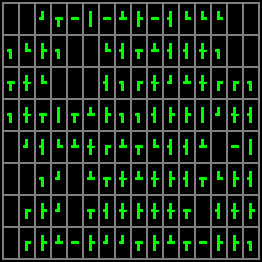
\includegraphics[scale=0.75]{\CURPATH/shuffled.png}
\caption{Разобранная головоломка}
\end{figure}

\dots и собранная:

\begin{figure}[H]
\label{fig:pipe_solved}
\centering
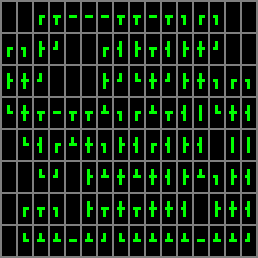
\includegraphics[scale=0.75]{\CURPATH/solved.png}
\caption{Собранная головоломка}
\end{figure}

Попробуем найти способ собрать её.

\subsubsection{Создание}

В начале, нужно её создать.
Вот простая идея.
Возьем массив ячеек 8*16.
Каждая ячейка может содержать какой-то тип блока.
Между ячейками есть стыки:

\pgfmathsetmacro\Width{16}
\pgfmathsetmacro\Height{8}
%\pgfmathsetmacro\Width{10}
%\pgfmathsetmacro\Height{5}
\pgfmathtruncatemacro\WidthMinusI{\Width - 1}
\pgfmathtruncatemacro\WidthMinusII{\Width - 2}
\pgfmathtruncatemacro\HeightMinusI{\Height - 1}
\pgfmathtruncatemacro\HeightMinusII{\Height - 2}
\pgfmathtruncatemacro\HeightPlusII{\Height + 2}
\pgfmathsetmacro\HeightPlusIi{\Height + 1.5}

% see also: http://www.texample.net/tikz/examples/euclid-algorithm/
\begin{center}
\begin{tikzpicture}[set style={{help lines}+=[dashed]},scale=0.7]

	\draw[style=help lines] (0,0) grid +(\Width,\Height);

	\foreach \c in {0,...,\WidthMinusI}
	{
		\foreach \r in {0,...,\HeightMinusII}
			\draw   [red,very thick,-] (\c+0.5,\r+0.75) -- (\c+0.5,\r+1.25);
		%\node[rotate=90] at (\c+0.5,\HeightPlusII) {\Large vjoints[\dots, \c] \normalsize};
		\node[rotate=90] at (\c+0.5,\HeightPlusII) {vjoints[\dots, \c]};
	}

	\foreach \r in {0,...,\HeightMinusI}
	{
		\foreach \c in {0,...,\WidthMinusII}
			\draw   [blue,very thick,-] (\c+0.75,\r+0.5) -- (\c+1.25,\r+0.5);
		\pgfmathtruncatemacro\hjointslabel{\HeightMinusI - \r}
		%\node at (-1.5,\r+0.5) {\large hjoints[\hjointslabel, \dots] \normalsize};
		\node at (-1.5,\r+0.5) {hjoints[\hjointslabel, \dots]};
	}

\end{tikzpicture}
\end{center}



Синие линии это горизонтальные стыки, красные линии это вертикальные стыки.
Мы просто случайно выставляем каждый стык в 0/false (отсутствует) или 1/true (присутствует).

После этого, теперь легко найти тип каждой ячейки.
А это:

\newcommand{\HeaderColor}{\cellcolor{blue!25}}
\begin{center}
\begin{longtable}{ | l | l | l | l | }
\hline
\HeaderColor стыки & \HeaderColor наше внутреннее название & \HeaderColor угол & \HeaderColor символ \\
\hline
0	&type 0		&	0$^{\circ}$	& (пробел)	\\
2	&type 2a	&	0$^{\circ}$	& \pmboxdrawuni{2503} \\ % ┃
2	&type 2a	&	90$^{\circ}$	& \pmboxdrawuni{2501} \\ % ━
2	&type 2b	&	0$^{\circ}$	& \pmboxdrawuni{250F} \\ % ┏
2	&type 2b	&	90$^{\circ}$	& \pmboxdrawuni{2513} \\ % ┓
2	&type 2b	&	180$^{\circ}$	& \pmboxdrawuni{251B} \\ % ┛
2	&type 2b	&	270$^{\circ}$	& \pmboxdrawuni{2517} \\ % ┗
3	&type 3		&	0$^{\circ}$	& \pmboxdrawuni{2523} \\ % ┣
3 	&type 3		&	90$^{\circ}$	& \pmboxdrawuni{2533} \\ % ┳
3	&type 3		&	180$^{\circ}$	& \pmboxdrawuni{252B} \\ % ┫
3	&type 3		&	270$^{\circ}$	& \pmboxdrawuni{253B} \\ % ┻
4	&type 4		&	0$^{\circ}$	& \pmboxdrawuni{254B} \\ % ╋
\hline
\end{longtable}
\end{center}

\textit{Висящие} стыки могут присутствовать на первой стадии (т.е., ячейки только с одним стыком), но они удалются
рекурсивно, и эти ячейки преобразуются в пустые ячейки.
Так что, в самом конце, все ячейки имеют минимум 2 стыка, и вся эта сантехническая система не имеет связей с внешним миром ---
я надеюсь, из-за этого станет немного проще.

Исходник генератора на Си здесь: \url{.../pipe/generator}.
Все вертикальные стыки хранятся в глобальном массиве \textit{hjoints[]} и вертикальные в \textit{vjoints[]}.

Программа на Си генерирует ANSI-раскрашенный вывод, как это было показано выше
(\ref{fig:pipe_shuffled}, \ref{fig:pipe_solved}) плюс массив типов для каждой ячейки, но без информации об углах:

\begin{lstlisting}[label=init_cells]
[
["0", "0", "2b", "3", "2a", "2a", "2a", "3", "3", "2a", "3", "2b", "2b", "2b", "0", "0"],
["2b", "2b", "3", "2b", "0", "0", "2b", "3", "3", "3", "3", "3", "4", "2b", "0", "0"],
["3", "4", "2b", "0", "0", "0", "3", "2b", "2b", "4", "2b", "3", "4", "2b", "2b", "2b"],
["2b", "4", "3", "2a", "3", "3", "3", "2b", "2b", "3", "3", "3", "2a", "2b", "4", "3"],
["0", "2b", "3", "2b", "3", "4", "2b", "3", "3", "2b", "3", "3", "3", "0", "2a", "2a"],
["0", "0", "2b", "2b", "0", "3", "3", "4", "3", "4", "3", "3", "3", "2b", "3", "3"],
["0", "2b", "3", "2b", "0", "3", "3", "4", "3", "4", "4", "3", "0", "3", "4", "3"],
["0", "2b", "3", "3", "2a", "3", "2b", "2b", "3", "3", "3", "3", "2a", "3", "3", "2b"],
]
\end{lstlisting}

\subsubsection{Решение}

Прежде всего, мы будем работать с массивом ячеек 8*16, где каждый элемент имеет 4 бита:
``T'' (top/верх),
``B'' (bottom/низ),
``L'' (left/лево),
``R'' (right/право).
Каждый бит представляет собой половину стыка.

% see also: http://www.texample.net/tikz/examples/euclid-algorithm/
\begin{center}
\begin{tikzpicture}[set style={{help lines}+=[dashed]},scale=0.7]

	\draw[style=help lines] (0,0) grid +(\Width,\Height);
	
	\foreach \c in {0,...,\WidthMinusI}
		%\node[rotate=90] at (\c+0.5,\HeightPlusIi) {\Large [\dots, \c] \normalsize};
		\node[rotate=90] at (\c+0.5,\HeightPlusIi) {[\dots, \c]};
	
	\foreach \r in {0,...,\HeightMinusI}
	{
		\pgfmathtruncatemacro\hlabel{\HeightMinusI - \r}
		%\node at (-1.5,\r+0.5) {\large [\hlabel, \dots] \normalsize};
		\node at (-1.5,\r+0.5) {[\hlabel, \dots]};
	
		\pgfmathsetmacro\Shift{0.325}
		\foreach \c in {0,...,\WidthMinusI}
		{
			\node at (\c+0.5,\r+0.5 + \Shift) {\footnotesize T \normalsize};
			\node at (\c+0.5,\r+0.5 - \Shift) {\footnotesize B \normalsize};
			\node at (\c+0.5 - \Shift,\r+0.5) {\footnotesize L \normalsize};
			\node at (\c+0.5 + \Shift,\r+0.5) {\footnotesize R \normalsize};
		}
	}

\end{tikzpicture}
\end{center}


Теперь определяем массив для каждого из четырех полустыков + информация об угле:

\begin{lstlisting}
HEIGHT=8
WIDTH=16

# if T/B/R/L is Bool instead of Int, Z3 solver will work faster
T=[[Bool('cell_%d_%d_top' % (r, c)) for c in range(WIDTH)] for r in range(HEIGHT)]
B=[[Bool('cell_%d_%d_bottom' % (r, c)) for c in range(WIDTH)] for r in range(HEIGHT)]
R=[[Bool('cell_%d_%d_right' % (r, c)) for c in range(WIDTH)] for r in range(HEIGHT)]
L=[[Bool('cell_%d_%d_left' % (r, c)) for c in range(WIDTH)] for r in range(HEIGHT)]
A=[[Int('cell_%d_%d_angle' % (r, c)) for c in range(WIDTH)] for r in range(HEIGHT)]
\end{lstlisting}

Мы знаем, что если каждый из полустыков присутствует, ответный полустык также должен присутствовать, и наоборот. 
Определяем всё это используя эти констрайнты:

\begin{lstlisting}
# shorthand variables for True and False:
t=True
f=False

# "top" of each cell must be equal to "bottom" of the cell above
# "bottom" of each cell must be equal to "top" of the cell below
# "left" of each cell must be equal to "right" of the cell at left
# "right" of each cell must be equal to "left" of the cell at right
for r in range(HEIGHT):
    for c in range(WIDTH):
        if r!=0:
            s.add(T[r][c]==B[r-1][c])
        if r!=HEIGHT-1:
            s.add(B[r][c]==T[r+1][c])
        if c!=0:
            s.add(L[r][c]==R[r][c-1])
        if c!=WIDTH-1:
            s.add(R[r][c]==L[r][c+1])

# "left" of each cell of first column shouldn't have any connection
# so is "right" of each cell of the last column
for r in range(HEIGHT):
    s.add(L[r][0]==f)
    s.add(R[r][WIDTH-1]==f)

# "top" of each cell of the first row shouldn't have any connection
# so is "bottom" of each cell of the last row
for c in range(WIDTH):
    s.add(T[0][c]==f)
    s.add(B[HEIGHT-1][c]==f)
\end{lstlisting}

Теперь перебираем все ячейки в изначальном массиве (\ref{init_cells}).
Первые две ячейки здесь пустые. И третья имеет тип ``2b''.
Это ``\pmboxdrawuni{250F}'' % ┏
и его можно ориентировать четырьмя разными способами.
И если её угол это 0$^{\circ}$, верхний и правый полустыки присутствуют, остальные отсутствуют.
Если он имеет угол 90$^{\circ}$, он выглядит как 
``\pmboxdrawuni{2513}'', % ┓
и верхник и левый полустыки присутствуют, остальные отсутствуют.

На обычном русском языке: ``если ячейка этого типа имеет угол 0$^{\circ}$, вот эти полустыки должны присутствовать \textbf{ИЛИ}
если она имеет угол 90$^{\circ}$, эти полустыки должны присутствовать, \textbf{ИЛИ}, итд, итд.''

Точно также, мы определяем эти правила для всех типов и всех возможных углов:

\begin{lstlisting}
for r in range(HEIGHT):
    for c in range(WIDTH):
        ty=cells_type[r][c]

        if ty=="0":
            s.add(A[r][c]==f)
            s.add(T[r][c]==f, B[r][c]==f, L[r][c]==f, R[r][c]==f)

        if ty=="2a":
            s.add(Or(And(A[r][c]==0, L[r][c]==f, R[r][c]==f, T[r][c]==t, B[r][c]==t),   # §\pmboxdrawuni{2503}§
                    And(A[r][c]==90, L[r][c]==t, R[r][c]==t, T[r][c]==f, B[r][c]==f)))  # §\pmboxdrawuni{2501}§

        if ty=="2b":
            s.add(Or(And(A[r][c]==0, L[r][c]==f, R[r][c]==t, T[r][c]==f, B[r][c]==t),   # §\pmboxdrawuni{250F}§
                    And(A[r][c]==90, L[r][c]==t, R[r][c]==f, T[r][c]==f, B[r][c]==t),   # §\pmboxdrawuni{2513}§
                    And(A[r][c]==180, L[r][c]==t, R[r][c]==f, T[r][c]==t, B[r][c]==f),  # §\pmboxdrawuni{251B}§
                    And(A[r][c]==270, L[r][c]==f, R[r][c]==t, T[r][c]==t, B[r][c]==f))) # §\pmboxdrawuni{2517}§
	
        if ty=="3":
            s.add(Or(And(A[r][c]==0, L[r][c]==f, R[r][c]==t, T[r][c]==t, B[r][c]==t),   # §\pmboxdrawuni{2523}§
                    And(A[r][c]==90, L[r][c]==t, R[r][c]==t, T[r][c]==f, B[r][c]==t),   # §\pmboxdrawuni{2533}§
                    And(A[r][c]==180, L[r][c]==t, R[r][c]==f, T[r][c]==t, B[r][c]==t),  # §\pmboxdrawuni{252B}§
                    And(A[r][c]==270, L[r][c]==t, R[r][c]==t, T[r][c]==t, B[r][c]==f))) # §\pmboxdrawuni{253B}§

        if ty=="4":
            s.add(A[r][c]==0)
            s.add(T[r][c]==t, B[r][c]==t, L[r][c]==t, R[r][c]==t) # §\pmboxdrawuni{254B}§
\end{lstlisting}

Полный исходник здесь: \url{.../solver/solve_pipe_puzzle1.py}.

Получается такой результат (выводит угол для каждой ячейки и (псевдо)графическое представление):

\begin{figure}[H]
\centering
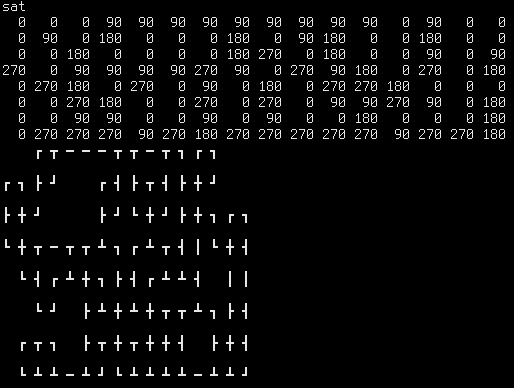
\includegraphics[scale=0.75]{\CURPATH/solver/solver.png}
\caption{Вывод скрипта солвера}
\end{figure}

Это работает $\approx 4$ секунды на моем старом и медленном Intel Atom N455 1.66GHz.
Быстро ли это? Не знаю, но снова вот что действительно круто, это то что мы понятия не имеем о какой-то математической
теории за всем этим, мы просто объявили ячейки, (полу-)стыки и определили отношения между ними.

Теперь следующий вопрос это, сколько здесь возможных решений?
Используя раннее описанный метод (\ref{SMTEnumerate}), я немного изменил скрипт солвера
\footnote{\url{.../solver/solve_pipe_puzzle2.py}} и солвер
сказал что возможно два решения.

Сравним их используя gvimdiff:

\begin{figure}[H]
\centering
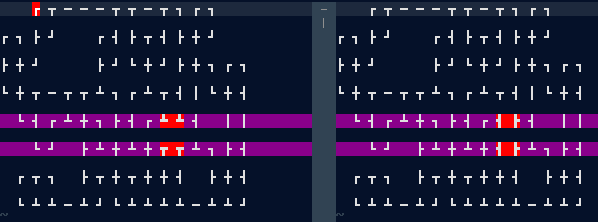
\includegraphics[scale=0.75]{\CURPATH/solver/diff.png}
\caption{Вывод gvimdiff (извините за мой красный курсор в левой части в левом верхнем углу)}
\end{figure}

4 ячейки в середине могут быть ориентированы по-разному.
Видимо, другие головоломки могут также выдавать разные результаты.

P.S.
\textit{Полу-стык} определен как булевый тип.
Но на самом деле, первая версия солвера была написана используя целочисленный тип для полу-стыков,
и 0 использовалось для False и 1 для True.
Я так сделал, потому что хотел более компактный исходный код, без использования длинных слов как ``False'' и ``True''.
И это работало, но медленнее. Вероятно, Z3 работает с булевыми типами быстрее? Лучше?
Так или иначе, я пишу это чтобы отметить, что, если нужно, целочисленный тип можно использовать вместо булевого.


\section{Развлекательная математика и головоломки}

\subsection{Судоку}

Головоломка Судоку это решетка 9*9, некоторые ячейки заполнены значениями, некоторые пустые:

% copypasted from http://www.texample.net/tikz/examples/sudoku/
\newcounter{row}
\newcounter{col}

\newcommand\setrow[9]{
  \setcounter{col}{1}
  \foreach \n in {#1, #2, #3, #4, #5, #6, #7, #8, #9} {
    \edef\x{\value{col} - 0.5}
    \edef\y{9.5 - \value{row}}
    \node[anchor=center] at (\x, \y) {\n};
    \stepcounter{col}
  }
  \stepcounter{row}
}

\begin{center}
\begin{tikzpicture}[scale=.7]
  \begin{scope}
    \draw (0, 0) grid (9, 9);
    \draw[very thick, scale=3] (0, 0) grid (3, 3);

    \setcounter{row}{1}
    \setrow { }{ }{5}  {3}{ }{ }  { }{ }{ }
    \setrow {8}{ }{ }  { }{ }{ }  { }{2}{ }
    \setrow { }{7}{ }  { }{1}{ }  {5}{ }{ }

    \setrow {4}{ }{ }  { }{ }{5}  {3}{ }{ }
    \setrow { }{1}{ }  { }{7}{ }  { }{ }{6}
    \setrow { }{ }{3}  {2}{ }{ }  { }{8}{ }

    \setrow { }{6}{ }  {5}{ }{ }  { }{ }{9}
    \setrow { }{ }{4}  { }{ }{ }  { }{3}{ }
    \setrow { }{ }{ }  { }{ }{9}  {7}{ }{ }

    \node[anchor=center] at (4.5, -0.5) {Нерешенная Судоку};
  \end{scope}
\end{tikzpicture}
\end{center}

Числа в каждом ряду должны быть уникальными, т.е., каждый ряд должен содержать 9 чисел в пределах 1..9 без повторений.
Та же история и для каждого столбца и каждого квадрата 3*3.

Головоломка представляет собой хороший кандидат, на котором можно попробовать \ac{SMT}-солвер, потому что это,
в общем-то, просто нерешенная система уравнений.

\input{puzzles/sudoku/1/main_RU}
%\input{puzzles/sudoku/GT/main_RU}
%\input{puzzles/sudoku/killer/main_RU}
\input{puzzles/sudoku/KLEE/main_RU}
\input{puzzles/sudoku/SAT/main_RU}


\subsection{Головоломка зебры (\ac{AKA} Загадка Эйнштейна)}

\input{puzzles/zebra/SMT/main_RU}
\input{puzzles/zebra/KLEE/main_RU}
\input{puzzles/zebra/SAT/main_RU}


\subsection{Решение головоломки ``трубы'' используя Z3 SMT-солвер}

\renewcommand{\CURPATH}{puzzles/pipe}

Головоломка ``трубы'' это популярная головоломка (просто погуглите ``pipe puzzle'' и посмотрите на картинки).

Вот как выглядит головоломка в разобранном виде:

\begin{figure}[H]
\label{fig:pipe_shuffled}
\centering
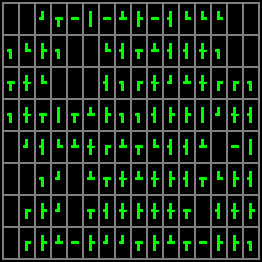
\includegraphics[scale=0.75]{\CURPATH/shuffled.png}
\caption{Разобранная головоломка}
\end{figure}

\dots и собранная:

\begin{figure}[H]
\label{fig:pipe_solved}
\centering
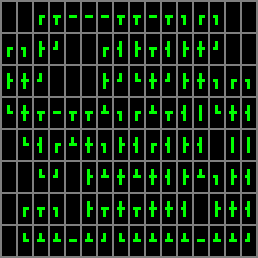
\includegraphics[scale=0.75]{\CURPATH/solved.png}
\caption{Собранная головоломка}
\end{figure}

Попробуем найти способ собрать её.

\subsubsection{Создание}

В начале, нужно её создать.
Вот простая идея.
Возьем массив ячеек 8*16.
Каждая ячейка может содержать какой-то тип блока.
Между ячейками есть стыки:

\input{\CURPATH/pipe_gen.tex}

Синие линии это горизонтальные стыки, красные линии это вертикальные стыки.
Мы просто случайно выставляем каждый стык в 0/false (отсутствует) или 1/true (присутствует).

После этого, теперь легко найти тип каждой ячейки.
А это:

\newcommand{\HeaderColor}{\cellcolor{blue!25}}
\begin{center}
\begin{longtable}{ | l | l | l | l | }
\hline
\HeaderColor стыки & \HeaderColor наше внутреннее название & \HeaderColor угол & \HeaderColor символ \\
\hline
0	&type 0		&	0$^{\circ}$	& (пробел)	\\
2	&type 2a	&	0$^{\circ}$	& \pmboxdrawuni{2503} \\ % ┃
2	&type 2a	&	90$^{\circ}$	& \pmboxdrawuni{2501} \\ % ━
2	&type 2b	&	0$^{\circ}$	& \pmboxdrawuni{250F} \\ % ┏
2	&type 2b	&	90$^{\circ}$	& \pmboxdrawuni{2513} \\ % ┓
2	&type 2b	&	180$^{\circ}$	& \pmboxdrawuni{251B} \\ % ┛
2	&type 2b	&	270$^{\circ}$	& \pmboxdrawuni{2517} \\ % ┗
3	&type 3		&	0$^{\circ}$	& \pmboxdrawuni{2523} \\ % ┣
3 	&type 3		&	90$^{\circ}$	& \pmboxdrawuni{2533} \\ % ┳
3	&type 3		&	180$^{\circ}$	& \pmboxdrawuni{252B} \\ % ┫
3	&type 3		&	270$^{\circ}$	& \pmboxdrawuni{253B} \\ % ┻
4	&type 4		&	0$^{\circ}$	& \pmboxdrawuni{254B} \\ % ╋
\hline
\end{longtable}
\end{center}

\textit{Висящие} стыки могут присутствовать на первой стадии (т.е., ячейки только с одним стыком), но они удалются
рекурсивно, и эти ячейки преобразуются в пустые ячейки.
Так что, в самом конце, все ячейки имеют минимум 2 стыка, и вся эта сантехническая система не имеет связей с внешним миром ---
я надеюсь, из-за этого станет немного проще.

Исходник генератора на Си здесь: \url{.../pipe/generator}.
Все вертикальные стыки хранятся в глобальном массиве \textit{hjoints[]} и вертикальные в \textit{vjoints[]}.

Программа на Си генерирует ANSI-раскрашенный вывод, как это было показано выше
(\ref{fig:pipe_shuffled}, \ref{fig:pipe_solved}) плюс массив типов для каждой ячейки, но без информации об углах:

\begin{lstlisting}[label=init_cells]
[
["0", "0", "2b", "3", "2a", "2a", "2a", "3", "3", "2a", "3", "2b", "2b", "2b", "0", "0"],
["2b", "2b", "3", "2b", "0", "0", "2b", "3", "3", "3", "3", "3", "4", "2b", "0", "0"],
["3", "4", "2b", "0", "0", "0", "3", "2b", "2b", "4", "2b", "3", "4", "2b", "2b", "2b"],
["2b", "4", "3", "2a", "3", "3", "3", "2b", "2b", "3", "3", "3", "2a", "2b", "4", "3"],
["0", "2b", "3", "2b", "3", "4", "2b", "3", "3", "2b", "3", "3", "3", "0", "2a", "2a"],
["0", "0", "2b", "2b", "0", "3", "3", "4", "3", "4", "3", "3", "3", "2b", "3", "3"],
["0", "2b", "3", "2b", "0", "3", "3", "4", "3", "4", "4", "3", "0", "3", "4", "3"],
["0", "2b", "3", "3", "2a", "3", "2b", "2b", "3", "3", "3", "3", "2a", "3", "3", "2b"],
]
\end{lstlisting}

\subsubsection{Решение}

Прежде всего, мы будем работать с массивом ячеек 8*16, где каждый элемент имеет 4 бита:
``T'' (top/верх),
``B'' (bottom/низ),
``L'' (left/лево),
``R'' (right/право).
Каждый бит представляет собой половину стыка.

\input{\CURPATH/pipe_solve.tex}

Теперь определяем массив для каждого из четырех полустыков + информация об угле:

\begin{lstlisting}
HEIGHT=8
WIDTH=16

# if T/B/R/L is Bool instead of Int, Z3 solver will work faster
T=[[Bool('cell_%d_%d_top' % (r, c)) for c in range(WIDTH)] for r in range(HEIGHT)]
B=[[Bool('cell_%d_%d_bottom' % (r, c)) for c in range(WIDTH)] for r in range(HEIGHT)]
R=[[Bool('cell_%d_%d_right' % (r, c)) for c in range(WIDTH)] for r in range(HEIGHT)]
L=[[Bool('cell_%d_%d_left' % (r, c)) for c in range(WIDTH)] for r in range(HEIGHT)]
A=[[Int('cell_%d_%d_angle' % (r, c)) for c in range(WIDTH)] for r in range(HEIGHT)]
\end{lstlisting}

Мы знаем, что если каждый из полустыков присутствует, ответный полустык также должен присутствовать, и наоборот. 
Определяем всё это используя эти констрайнты:

\begin{lstlisting}
# shorthand variables for True and False:
t=True
f=False

# "top" of each cell must be equal to "bottom" of the cell above
# "bottom" of each cell must be equal to "top" of the cell below
# "left" of each cell must be equal to "right" of the cell at left
# "right" of each cell must be equal to "left" of the cell at right
for r in range(HEIGHT):
    for c in range(WIDTH):
        if r!=0:
            s.add(T[r][c]==B[r-1][c])
        if r!=HEIGHT-1:
            s.add(B[r][c]==T[r+1][c])
        if c!=0:
            s.add(L[r][c]==R[r][c-1])
        if c!=WIDTH-1:
            s.add(R[r][c]==L[r][c+1])

# "left" of each cell of first column shouldn't have any connection
# so is "right" of each cell of the last column
for r in range(HEIGHT):
    s.add(L[r][0]==f)
    s.add(R[r][WIDTH-1]==f)

# "top" of each cell of the first row shouldn't have any connection
# so is "bottom" of each cell of the last row
for c in range(WIDTH):
    s.add(T[0][c]==f)
    s.add(B[HEIGHT-1][c]==f)
\end{lstlisting}

Теперь перебираем все ячейки в изначальном массиве (\ref{init_cells}).
Первые две ячейки здесь пустые. И третья имеет тип ``2b''.
Это ``\pmboxdrawuni{250F}'' % ┏
и его можно ориентировать четырьмя разными способами.
И если её угол это 0$^{\circ}$, верхний и правый полустыки присутствуют, остальные отсутствуют.
Если он имеет угол 90$^{\circ}$, он выглядит как 
``\pmboxdrawuni{2513}'', % ┓
и верхник и левый полустыки присутствуют, остальные отсутствуют.

На обычном русском языке: ``если ячейка этого типа имеет угол 0$^{\circ}$, вот эти полустыки должны присутствовать \textbf{ИЛИ}
если она имеет угол 90$^{\circ}$, эти полустыки должны присутствовать, \textbf{ИЛИ}, итд, итд.''

Точно также, мы определяем эти правила для всех типов и всех возможных углов:

\begin{lstlisting}
for r in range(HEIGHT):
    for c in range(WIDTH):
        ty=cells_type[r][c]

        if ty=="0":
            s.add(A[r][c]==f)
            s.add(T[r][c]==f, B[r][c]==f, L[r][c]==f, R[r][c]==f)

        if ty=="2a":
            s.add(Or(And(A[r][c]==0, L[r][c]==f, R[r][c]==f, T[r][c]==t, B[r][c]==t),   # §\pmboxdrawuni{2503}§
                    And(A[r][c]==90, L[r][c]==t, R[r][c]==t, T[r][c]==f, B[r][c]==f)))  # §\pmboxdrawuni{2501}§

        if ty=="2b":
            s.add(Or(And(A[r][c]==0, L[r][c]==f, R[r][c]==t, T[r][c]==f, B[r][c]==t),   # §\pmboxdrawuni{250F}§
                    And(A[r][c]==90, L[r][c]==t, R[r][c]==f, T[r][c]==f, B[r][c]==t),   # §\pmboxdrawuni{2513}§
                    And(A[r][c]==180, L[r][c]==t, R[r][c]==f, T[r][c]==t, B[r][c]==f),  # §\pmboxdrawuni{251B}§
                    And(A[r][c]==270, L[r][c]==f, R[r][c]==t, T[r][c]==t, B[r][c]==f))) # §\pmboxdrawuni{2517}§
	
        if ty=="3":
            s.add(Or(And(A[r][c]==0, L[r][c]==f, R[r][c]==t, T[r][c]==t, B[r][c]==t),   # §\pmboxdrawuni{2523}§
                    And(A[r][c]==90, L[r][c]==t, R[r][c]==t, T[r][c]==f, B[r][c]==t),   # §\pmboxdrawuni{2533}§
                    And(A[r][c]==180, L[r][c]==t, R[r][c]==f, T[r][c]==t, B[r][c]==t),  # §\pmboxdrawuni{252B}§
                    And(A[r][c]==270, L[r][c]==t, R[r][c]==t, T[r][c]==t, B[r][c]==f))) # §\pmboxdrawuni{253B}§

        if ty=="4":
            s.add(A[r][c]==0)
            s.add(T[r][c]==t, B[r][c]==t, L[r][c]==t, R[r][c]==t) # §\pmboxdrawuni{254B}§
\end{lstlisting}

Полный исходник здесь: \url{.../solver/solve_pipe_puzzle1.py}.

Получается такой результат (выводит угол для каждой ячейки и (псевдо)графическое представление):

\begin{figure}[H]
\centering
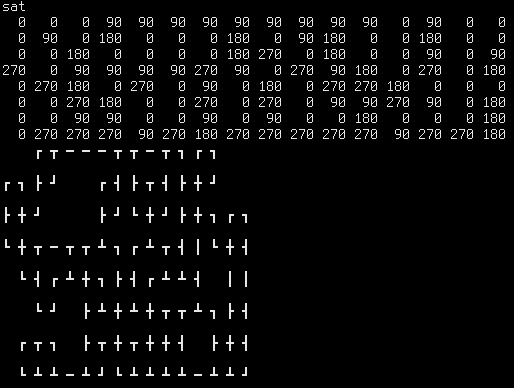
\includegraphics[scale=0.75]{\CURPATH/solver/solver.png}
\caption{Вывод скрипта солвера}
\end{figure}

Это работает $\approx 4$ секунды на моем старом и медленном Intel Atom N455 1.66GHz.
Быстро ли это? Не знаю, но снова вот что действительно круто, это то что мы понятия не имеем о какой-то математической
теории за всем этим, мы просто объявили ячейки, (полу-)стыки и определили отношения между ними.

Теперь следующий вопрос это, сколько здесь возможных решений?
Используя раннее описанный метод (\ref{SMTEnumerate}), я немного изменил скрипт солвера
\footnote{\url{.../solver/solve_pipe_puzzle2.py}} и солвер
сказал что возможно два решения.

Сравним их используя gvimdiff:

\begin{figure}[H]
\centering
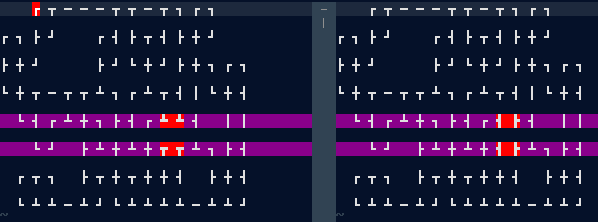
\includegraphics[scale=0.75]{\CURPATH/solver/diff.png}
\caption{Вывод gvimdiff (извините за мой красный курсор в левой части в левом верхнем углу)}
\end{figure}

4 ячейки в середине могут быть ориентированы по-разному.
Видимо, другие головоломки могут также выдавать разные результаты.

P.S.
\textit{Полу-стык} определен как булевый тип.
Но на самом деле, первая версия солвера была написана используя целочисленный тип для полу-стыков,
и 0 использовалось для False и 1 для True.
Я так сделал, потому что хотел более компактный исходный код, без использования длинных слов как ``False'' и ``True''.
И это работало, но медленнее. Вероятно, Z3 работает с булевыми типами быстрее? Лучше?
Так или иначе, я пишу это чтобы отметить, что, если нужно, целочисленный тип можно использовать вместо булевого.


\section{Развлекательная математика и головоломки}

\input{puzzles/sudoku/main_RU}
\input{puzzles/zebra/main_RU}
\input{puzzles/pipe/main_RU}
\input{puzzles/rubik2/failed_SMT/main_RU}
\input{puzzles/rubik2/SAT/main_RU}
\input{puzzles/rubik3/one_face_SMT/main_RU}
%\input{puzzles/numberlink/main_RU}
%\input{puzzles/two_parks_RU}
\input{puzzles/alphametics/main_RU}
%\input{puzzles/2015_AIME_II_Problems_12_RU}
%\input{puzzles/fred/main_RU}
%\input{puzzles/MC/main_RU}
%\input{puzzles/coin_flip/main_RU}
%\input{puzzles/Mock_AIME_2_2006-2007_Problem_8_RU}
%\input{puzzles/2012_AIME_I_Problems_1_RU}
%\input{puzzles/keypad_RU}


\section{Развлекательная математика и головоломки}

\input{puzzles/sudoku/main_RU}
\input{puzzles/zebra/main_RU}
\input{puzzles/pipe/main_RU}
\input{puzzles/rubik2/failed_SMT/main_RU}
\input{puzzles/rubik2/SAT/main_RU}
\input{puzzles/rubik3/one_face_SMT/main_RU}
%\input{puzzles/numberlink/main_RU}
%\input{puzzles/two_parks_RU}
\input{puzzles/alphametics/main_RU}
%\input{puzzles/2015_AIME_II_Problems_12_RU}
%\input{puzzles/fred/main_RU}
%\input{puzzles/MC/main_RU}
%\input{puzzles/coin_flip/main_RU}
%\input{puzzles/Mock_AIME_2_2006-2007_Problem_8_RU}
%\input{puzzles/2012_AIME_I_Problems_1_RU}
%\input{puzzles/keypad_RU}


\section{Развлекательная математика и головоломки}

\input{puzzles/sudoku/main_RU}
\input{puzzles/zebra/main_RU}
\input{puzzles/pipe/main_RU}
\input{puzzles/rubik2/failed_SMT/main_RU}
\input{puzzles/rubik2/SAT/main_RU}
\input{puzzles/rubik3/one_face_SMT/main_RU}
%\input{puzzles/numberlink/main_RU}
%\input{puzzles/two_parks_RU}
\input{puzzles/alphametics/main_RU}
%\input{puzzles/2015_AIME_II_Problems_12_RU}
%\input{puzzles/fred/main_RU}
%\input{puzzles/MC/main_RU}
%\input{puzzles/coin_flip/main_RU}
%\input{puzzles/Mock_AIME_2_2006-2007_Problem_8_RU}
%\input{puzzles/2012_AIME_I_Problems_1_RU}
%\input{puzzles/keypad_RU}


%\section{Развлекательная математика и головоломки}

\input{puzzles/sudoku/main_RU}
\input{puzzles/zebra/main_RU}
\input{puzzles/pipe/main_RU}
\input{puzzles/rubik2/failed_SMT/main_RU}
\input{puzzles/rubik2/SAT/main_RU}
\input{puzzles/rubik3/one_face_SMT/main_RU}
%\input{puzzles/numberlink/main_RU}
%\input{puzzles/two_parks_RU}
\input{puzzles/alphametics/main_RU}
%\input{puzzles/2015_AIME_II_Problems_12_RU}
%\input{puzzles/fred/main_RU}
%\input{puzzles/MC/main_RU}
%\input{puzzles/coin_flip/main_RU}
%\input{puzzles/Mock_AIME_2_2006-2007_Problem_8_RU}
%\input{puzzles/2012_AIME_I_Problems_1_RU}
%\input{puzzles/keypad_RU}


%\input{puzzles/two_parks_RU}
\subsection{Альфаметика}

Согласно Дональду Кнуту, термин ``Альфаметика'' был придуман Дж. Эйч. Аш. Хантером.
Это головоломка: какие десятичные цифры в пределах 0..9 нужно присвоить каждой букве, чтобы это уравнение было справедливо?

\begin{lstlisting}
  SEND
+ MORE
 -----
 MONEY
\end{lstlisting}

Для Z3 это легко:

\lstinputlisting{puzzles/alphametics/alpha.py}

Вывод:

\begin{lstlisting}
sat
[E, = 5,
 S, = 9,
 M, = 1,
 N, = 6,
 D, = 7,
 R, = 8,
 O, = 0,
 Y = 2]
\end{lstlisting}

Вот еще одна, из \ac{TAOCP} том IV (\url{http://www-cs-faculty.stanford.edu/~uno/fasc2b.ps.gz}):

\lstinputlisting{puzzles/alphametics/alpha2.py}

\begin{lstlisting}
sat
[L, = 6,
 S, = 7,
 N, = 2,
 T, = 1,
 I, = 5,
 V = 3,
 A, = 8,
 R, = 9,
 O, = 4,
 TRIO = 1954,
 SONATA, = 742818,
 VIOLA, = 35468,
 VIOLIN, = 354652]
\end{lstlisting}

% TODO URL
Эту головоломку я нашел в примерах pySMT:

\lstinputlisting{puzzles/alphametics/alpha3.py}

\begin{lstlisting}
sat
[D = 5, R = 4, O = 3, E = 8, L = 6, W = 7, H = 2]
\end{lstlisting}

%%% 

Это упражнение Q209 из
[Companion to the Papers of Donald Knuth]\footnote{\url{http://www-cs-faculty.stanford.edu/~knuth/cp.html}}.

\begin{lstlisting}
 KNIFE
  FORK
 SPOON
  SOUP
------
SUPPER
\end{lstlisting}

В целях упрощения, я добавил ф-цию (list\_to\_expr()):

\lstinputlisting{puzzles/alphametics/alpha4.py}

\begin{lstlisting}
sat
[K = 7,
 N = 4,
 R = 9,
 I = 1,
 E = 6,
 S = 0,
 O = 3,
 F = 5,
 U = 8,
 P = 2,
 SUPPER = 82269,
 SOUP = 382,
 SPOON = 2334,
 FORK = 5397,
 KNIFE = 74156]
\end{lstlisting}

S это 0, так что значение SUPPER начинается с (убранного) нуля. Скажем так, нам это не нравится.
Добавим это, чтобы это исправить:

\begin{lstlisting}
s.add(S!=0)
\end{lstlisting}

\begin{lstlisting}
sat
[K = 8,
 N = 4,
 R = 3,
 I = 7,
 E = 6,
 S = 1,
 O = 9,
 F = 2,
 U = 0,
 P = 5,
 SUPPER = 105563,
 SOUP = 1905,
 SPOON = 15994,
 FORK = 2938,
 KNIFE = 84726]
\end{lstlisting}

\paragraph{Создание своей собственной головоломки}

Вот проблема: есть только 10 букв, но как их выбрать из числа слов?
Мы можем использовать Z3 для этого:

\lstinputlisting{puzzles/alphametics/gen.py}

Это первая сгенерированная головоломка:

\begin{lstlisting}
sat
EGGS
JELLY
LUNCH
C 5
E 6
G 3
H 7
J 0
L 1
N 4
S 8
U 2
Y 9
\end{lstlisting}

Что если мы хотим, чтобы слово ``CAKE'' присутствовало в числе ``слагаемых''?

Добавим это:

\begin{lstlisting}
s.add(word_used[words.index('CAKE')])
\end{lstlisting}

\begin{lstlisting}
sat
CAKE
TEA
LUNCH
A 8
C 3
E 1
H 9
J 6
K 2
L 0
N 5
T 7
U 4
\end{lstlisting}

Добавим это:

\begin{lstlisting}
s.add(word_used[words.index('EGGS')])
\end{lstlisting}

Теперь оно может найти пару к EGGS:

\begin{lstlisting}
sat
EGGS
HONEY
LUNCH
C 6
E 7
G 9
H 4
L 5
N 8
O 2
S 3
U 0
Y 1
\end{lstlisting}

\paragraph{Файлы}

\url{https://github.com/DennisYurichev/...}




%\input{puzzles/2015_AIME_II_Problems_12_RU}
%\section{Развлекательная математика и головоломки}

\input{puzzles/sudoku/main_RU}
\input{puzzles/zebra/main_RU}
\input{puzzles/pipe/main_RU}
\input{puzzles/rubik2/failed_SMT/main_RU}
\input{puzzles/rubik2/SAT/main_RU}
\input{puzzles/rubik3/one_face_SMT/main_RU}
%\input{puzzles/numberlink/main_RU}
%\input{puzzles/two_parks_RU}
\input{puzzles/alphametics/main_RU}
%\input{puzzles/2015_AIME_II_Problems_12_RU}
%\input{puzzles/fred/main_RU}
%\input{puzzles/MC/main_RU}
%\input{puzzles/coin_flip/main_RU}
%\input{puzzles/Mock_AIME_2_2006-2007_Problem_8_RU}
%\input{puzzles/2012_AIME_I_Problems_1_RU}
%\input{puzzles/keypad_RU}


%\section{Развлекательная математика и головоломки}

\input{puzzles/sudoku/main_RU}
\input{puzzles/zebra/main_RU}
\input{puzzles/pipe/main_RU}
\input{puzzles/rubik2/failed_SMT/main_RU}
\input{puzzles/rubik2/SAT/main_RU}
\input{puzzles/rubik3/one_face_SMT/main_RU}
%\input{puzzles/numberlink/main_RU}
%\input{puzzles/two_parks_RU}
\input{puzzles/alphametics/main_RU}
%\input{puzzles/2015_AIME_II_Problems_12_RU}
%\input{puzzles/fred/main_RU}
%\input{puzzles/MC/main_RU}
%\input{puzzles/coin_flip/main_RU}
%\input{puzzles/Mock_AIME_2_2006-2007_Problem_8_RU}
%\input{puzzles/2012_AIME_I_Problems_1_RU}
%\input{puzzles/keypad_RU}


%\section{Развлекательная математика и головоломки}

\input{puzzles/sudoku/main_RU}
\input{puzzles/zebra/main_RU}
\input{puzzles/pipe/main_RU}
\input{puzzles/rubik2/failed_SMT/main_RU}
\input{puzzles/rubik2/SAT/main_RU}
\input{puzzles/rubik3/one_face_SMT/main_RU}
%\input{puzzles/numberlink/main_RU}
%\input{puzzles/two_parks_RU}
\input{puzzles/alphametics/main_RU}
%\input{puzzles/2015_AIME_II_Problems_12_RU}
%\input{puzzles/fred/main_RU}
%\input{puzzles/MC/main_RU}
%\input{puzzles/coin_flip/main_RU}
%\input{puzzles/Mock_AIME_2_2006-2007_Problem_8_RU}
%\input{puzzles/2012_AIME_I_Problems_1_RU}
%\input{puzzles/keypad_RU}


%\input{puzzles/Mock_AIME_2_2006-2007_Problem_8_RU}
%\input{puzzles/2012_AIME_I_Problems_1_RU}
%\input{puzzles/keypad_RU}


\section{Развлекательная математика и головоломки}

\subsection{Судоку}

Головоломка Судоку это решетка 9*9, некоторые ячейки заполнены значениями, некоторые пустые:

% copypasted from http://www.texample.net/tikz/examples/sudoku/
\newcounter{row}
\newcounter{col}

\newcommand\setrow[9]{
  \setcounter{col}{1}
  \foreach \n in {#1, #2, #3, #4, #5, #6, #7, #8, #9} {
    \edef\x{\value{col} - 0.5}
    \edef\y{9.5 - \value{row}}
    \node[anchor=center] at (\x, \y) {\n};
    \stepcounter{col}
  }
  \stepcounter{row}
}

\begin{center}
\begin{tikzpicture}[scale=.7]
  \begin{scope}
    \draw (0, 0) grid (9, 9);
    \draw[very thick, scale=3] (0, 0) grid (3, 3);

    \setcounter{row}{1}
    \setrow { }{ }{5}  {3}{ }{ }  { }{ }{ }
    \setrow {8}{ }{ }  { }{ }{ }  { }{2}{ }
    \setrow { }{7}{ }  { }{1}{ }  {5}{ }{ }

    \setrow {4}{ }{ }  { }{ }{5}  {3}{ }{ }
    \setrow { }{1}{ }  { }{7}{ }  { }{ }{6}
    \setrow { }{ }{3}  {2}{ }{ }  { }{8}{ }

    \setrow { }{6}{ }  {5}{ }{ }  { }{ }{9}
    \setrow { }{ }{4}  { }{ }{ }  { }{3}{ }
    \setrow { }{ }{ }  { }{ }{9}  {7}{ }{ }

    \node[anchor=center] at (4.5, -0.5) {Нерешенная Судоку};
  \end{scope}
\end{tikzpicture}
\end{center}

Числа в каждом ряду должны быть уникальными, т.е., каждый ряд должен содержать 9 чисел в пределах 1..9 без повторений.
Та же история и для каждого столбца и каждого квадрата 3*3.

Головоломка представляет собой хороший кандидат, на котором можно попробовать \ac{SMT}-солвер, потому что это,
в общем-то, просто нерешенная система уравнений.

\input{puzzles/sudoku/1/main_RU}
%\input{puzzles/sudoku/GT/main_RU}
%\input{puzzles/sudoku/killer/main_RU}
\input{puzzles/sudoku/KLEE/main_RU}
\input{puzzles/sudoku/SAT/main_RU}


\subsection{Головоломка зебры (\ac{AKA} Загадка Эйнштейна)}

\input{puzzles/zebra/SMT/main_RU}
\input{puzzles/zebra/KLEE/main_RU}
\input{puzzles/zebra/SAT/main_RU}


\subsection{Решение головоломки ``трубы'' используя Z3 SMT-солвер}

\renewcommand{\CURPATH}{puzzles/pipe}

Головоломка ``трубы'' это популярная головоломка (просто погуглите ``pipe puzzle'' и посмотрите на картинки).

Вот как выглядит головоломка в разобранном виде:

\begin{figure}[H]
\label{fig:pipe_shuffled}
\centering
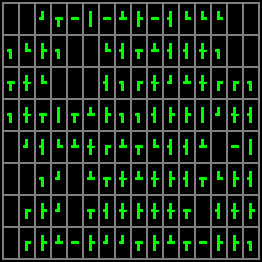
\includegraphics[scale=0.75]{\CURPATH/shuffled.png}
\caption{Разобранная головоломка}
\end{figure}

\dots и собранная:

\begin{figure}[H]
\label{fig:pipe_solved}
\centering
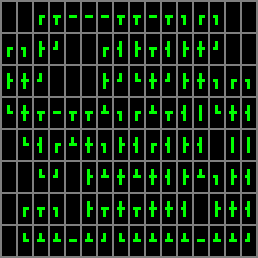
\includegraphics[scale=0.75]{\CURPATH/solved.png}
\caption{Собранная головоломка}
\end{figure}

Попробуем найти способ собрать её.

\subsubsection{Создание}

В начале, нужно её создать.
Вот простая идея.
Возьем массив ячеек 8*16.
Каждая ячейка может содержать какой-то тип блока.
Между ячейками есть стыки:

\input{\CURPATH/pipe_gen.tex}

Синие линии это горизонтальные стыки, красные линии это вертикальные стыки.
Мы просто случайно выставляем каждый стык в 0/false (отсутствует) или 1/true (присутствует).

После этого, теперь легко найти тип каждой ячейки.
А это:

\newcommand{\HeaderColor}{\cellcolor{blue!25}}
\begin{center}
\begin{longtable}{ | l | l | l | l | }
\hline
\HeaderColor стыки & \HeaderColor наше внутреннее название & \HeaderColor угол & \HeaderColor символ \\
\hline
0	&type 0		&	0$^{\circ}$	& (пробел)	\\
2	&type 2a	&	0$^{\circ}$	& \pmboxdrawuni{2503} \\ % ┃
2	&type 2a	&	90$^{\circ}$	& \pmboxdrawuni{2501} \\ % ━
2	&type 2b	&	0$^{\circ}$	& \pmboxdrawuni{250F} \\ % ┏
2	&type 2b	&	90$^{\circ}$	& \pmboxdrawuni{2513} \\ % ┓
2	&type 2b	&	180$^{\circ}$	& \pmboxdrawuni{251B} \\ % ┛
2	&type 2b	&	270$^{\circ}$	& \pmboxdrawuni{2517} \\ % ┗
3	&type 3		&	0$^{\circ}$	& \pmboxdrawuni{2523} \\ % ┣
3 	&type 3		&	90$^{\circ}$	& \pmboxdrawuni{2533} \\ % ┳
3	&type 3		&	180$^{\circ}$	& \pmboxdrawuni{252B} \\ % ┫
3	&type 3		&	270$^{\circ}$	& \pmboxdrawuni{253B} \\ % ┻
4	&type 4		&	0$^{\circ}$	& \pmboxdrawuni{254B} \\ % ╋
\hline
\end{longtable}
\end{center}

\textit{Висящие} стыки могут присутствовать на первой стадии (т.е., ячейки только с одним стыком), но они удалются
рекурсивно, и эти ячейки преобразуются в пустые ячейки.
Так что, в самом конце, все ячейки имеют минимум 2 стыка, и вся эта сантехническая система не имеет связей с внешним миром ---
я надеюсь, из-за этого станет немного проще.

Исходник генератора на Си здесь: \url{.../pipe/generator}.
Все вертикальные стыки хранятся в глобальном массиве \textit{hjoints[]} и вертикальные в \textit{vjoints[]}.

Программа на Си генерирует ANSI-раскрашенный вывод, как это было показано выше
(\ref{fig:pipe_shuffled}, \ref{fig:pipe_solved}) плюс массив типов для каждой ячейки, но без информации об углах:

\begin{lstlisting}[label=init_cells]
[
["0", "0", "2b", "3", "2a", "2a", "2a", "3", "3", "2a", "3", "2b", "2b", "2b", "0", "0"],
["2b", "2b", "3", "2b", "0", "0", "2b", "3", "3", "3", "3", "3", "4", "2b", "0", "0"],
["3", "4", "2b", "0", "0", "0", "3", "2b", "2b", "4", "2b", "3", "4", "2b", "2b", "2b"],
["2b", "4", "3", "2a", "3", "3", "3", "2b", "2b", "3", "3", "3", "2a", "2b", "4", "3"],
["0", "2b", "3", "2b", "3", "4", "2b", "3", "3", "2b", "3", "3", "3", "0", "2a", "2a"],
["0", "0", "2b", "2b", "0", "3", "3", "4", "3", "4", "3", "3", "3", "2b", "3", "3"],
["0", "2b", "3", "2b", "0", "3", "3", "4", "3", "4", "4", "3", "0", "3", "4", "3"],
["0", "2b", "3", "3", "2a", "3", "2b", "2b", "3", "3", "3", "3", "2a", "3", "3", "2b"],
]
\end{lstlisting}

\subsubsection{Решение}

Прежде всего, мы будем работать с массивом ячеек 8*16, где каждый элемент имеет 4 бита:
``T'' (top/верх),
``B'' (bottom/низ),
``L'' (left/лево),
``R'' (right/право).
Каждый бит представляет собой половину стыка.

\input{\CURPATH/pipe_solve.tex}

Теперь определяем массив для каждого из четырех полустыков + информация об угле:

\begin{lstlisting}
HEIGHT=8
WIDTH=16

# if T/B/R/L is Bool instead of Int, Z3 solver will work faster
T=[[Bool('cell_%d_%d_top' % (r, c)) for c in range(WIDTH)] for r in range(HEIGHT)]
B=[[Bool('cell_%d_%d_bottom' % (r, c)) for c in range(WIDTH)] for r in range(HEIGHT)]
R=[[Bool('cell_%d_%d_right' % (r, c)) for c in range(WIDTH)] for r in range(HEIGHT)]
L=[[Bool('cell_%d_%d_left' % (r, c)) for c in range(WIDTH)] for r in range(HEIGHT)]
A=[[Int('cell_%d_%d_angle' % (r, c)) for c in range(WIDTH)] for r in range(HEIGHT)]
\end{lstlisting}

Мы знаем, что если каждый из полустыков присутствует, ответный полустык также должен присутствовать, и наоборот. 
Определяем всё это используя эти констрайнты:

\begin{lstlisting}
# shorthand variables for True and False:
t=True
f=False

# "top" of each cell must be equal to "bottom" of the cell above
# "bottom" of each cell must be equal to "top" of the cell below
# "left" of each cell must be equal to "right" of the cell at left
# "right" of each cell must be equal to "left" of the cell at right
for r in range(HEIGHT):
    for c in range(WIDTH):
        if r!=0:
            s.add(T[r][c]==B[r-1][c])
        if r!=HEIGHT-1:
            s.add(B[r][c]==T[r+1][c])
        if c!=0:
            s.add(L[r][c]==R[r][c-1])
        if c!=WIDTH-1:
            s.add(R[r][c]==L[r][c+1])

# "left" of each cell of first column shouldn't have any connection
# so is "right" of each cell of the last column
for r in range(HEIGHT):
    s.add(L[r][0]==f)
    s.add(R[r][WIDTH-1]==f)

# "top" of each cell of the first row shouldn't have any connection
# so is "bottom" of each cell of the last row
for c in range(WIDTH):
    s.add(T[0][c]==f)
    s.add(B[HEIGHT-1][c]==f)
\end{lstlisting}

Теперь перебираем все ячейки в изначальном массиве (\ref{init_cells}).
Первые две ячейки здесь пустые. И третья имеет тип ``2b''.
Это ``\pmboxdrawuni{250F}'' % ┏
и его можно ориентировать четырьмя разными способами.
И если её угол это 0$^{\circ}$, верхний и правый полустыки присутствуют, остальные отсутствуют.
Если он имеет угол 90$^{\circ}$, он выглядит как 
``\pmboxdrawuni{2513}'', % ┓
и верхник и левый полустыки присутствуют, остальные отсутствуют.

На обычном русском языке: ``если ячейка этого типа имеет угол 0$^{\circ}$, вот эти полустыки должны присутствовать \textbf{ИЛИ}
если она имеет угол 90$^{\circ}$, эти полустыки должны присутствовать, \textbf{ИЛИ}, итд, итд.''

Точно также, мы определяем эти правила для всех типов и всех возможных углов:

\begin{lstlisting}
for r in range(HEIGHT):
    for c in range(WIDTH):
        ty=cells_type[r][c]

        if ty=="0":
            s.add(A[r][c]==f)
            s.add(T[r][c]==f, B[r][c]==f, L[r][c]==f, R[r][c]==f)

        if ty=="2a":
            s.add(Or(And(A[r][c]==0, L[r][c]==f, R[r][c]==f, T[r][c]==t, B[r][c]==t),   # §\pmboxdrawuni{2503}§
                    And(A[r][c]==90, L[r][c]==t, R[r][c]==t, T[r][c]==f, B[r][c]==f)))  # §\pmboxdrawuni{2501}§

        if ty=="2b":
            s.add(Or(And(A[r][c]==0, L[r][c]==f, R[r][c]==t, T[r][c]==f, B[r][c]==t),   # §\pmboxdrawuni{250F}§
                    And(A[r][c]==90, L[r][c]==t, R[r][c]==f, T[r][c]==f, B[r][c]==t),   # §\pmboxdrawuni{2513}§
                    And(A[r][c]==180, L[r][c]==t, R[r][c]==f, T[r][c]==t, B[r][c]==f),  # §\pmboxdrawuni{251B}§
                    And(A[r][c]==270, L[r][c]==f, R[r][c]==t, T[r][c]==t, B[r][c]==f))) # §\pmboxdrawuni{2517}§
	
        if ty=="3":
            s.add(Or(And(A[r][c]==0, L[r][c]==f, R[r][c]==t, T[r][c]==t, B[r][c]==t),   # §\pmboxdrawuni{2523}§
                    And(A[r][c]==90, L[r][c]==t, R[r][c]==t, T[r][c]==f, B[r][c]==t),   # §\pmboxdrawuni{2533}§
                    And(A[r][c]==180, L[r][c]==t, R[r][c]==f, T[r][c]==t, B[r][c]==t),  # §\pmboxdrawuni{252B}§
                    And(A[r][c]==270, L[r][c]==t, R[r][c]==t, T[r][c]==t, B[r][c]==f))) # §\pmboxdrawuni{253B}§

        if ty=="4":
            s.add(A[r][c]==0)
            s.add(T[r][c]==t, B[r][c]==t, L[r][c]==t, R[r][c]==t) # §\pmboxdrawuni{254B}§
\end{lstlisting}

Полный исходник здесь: \url{.../solver/solve_pipe_puzzle1.py}.

Получается такой результат (выводит угол для каждой ячейки и (псевдо)графическое представление):

\begin{figure}[H]
\centering
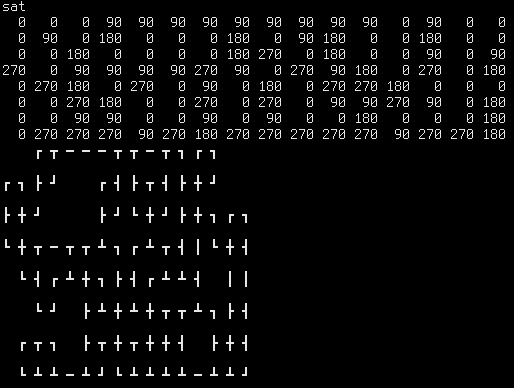
\includegraphics[scale=0.75]{\CURPATH/solver/solver.png}
\caption{Вывод скрипта солвера}
\end{figure}

Это работает $\approx 4$ секунды на моем старом и медленном Intel Atom N455 1.66GHz.
Быстро ли это? Не знаю, но снова вот что действительно круто, это то что мы понятия не имеем о какой-то математической
теории за всем этим, мы просто объявили ячейки, (полу-)стыки и определили отношения между ними.

Теперь следующий вопрос это, сколько здесь возможных решений?
Используя раннее описанный метод (\ref{SMTEnumerate}), я немного изменил скрипт солвера
\footnote{\url{.../solver/solve_pipe_puzzle2.py}} и солвер
сказал что возможно два решения.

Сравним их используя gvimdiff:

\begin{figure}[H]
\centering
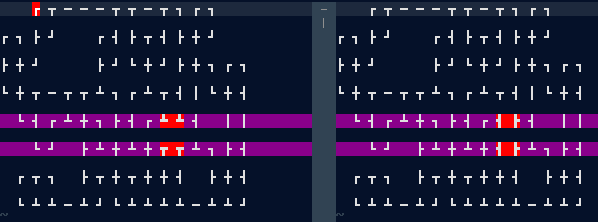
\includegraphics[scale=0.75]{\CURPATH/solver/diff.png}
\caption{Вывод gvimdiff (извините за мой красный курсор в левой части в левом верхнем углу)}
\end{figure}

4 ячейки в середине могут быть ориентированы по-разному.
Видимо, другие головоломки могут также выдавать разные результаты.

P.S.
\textit{Полу-стык} определен как булевый тип.
Но на самом деле, первая версия солвера была написана используя целочисленный тип для полу-стыков,
и 0 использовалось для False и 1 для True.
Я так сделал, потому что хотел более компактный исходный код, без использования длинных слов как ``False'' и ``True''.
И это работало, но медленнее. Вероятно, Z3 работает с булевыми типами быстрее? Лучше?
Так или иначе, я пишу это чтобы отметить, что, если нужно, целочисленный тип можно использовать вместо булевого.


\section{Развлекательная математика и головоломки}

\input{puzzles/sudoku/main_RU}
\input{puzzles/zebra/main_RU}
\input{puzzles/pipe/main_RU}
\input{puzzles/rubik2/failed_SMT/main_RU}
\input{puzzles/rubik2/SAT/main_RU}
\input{puzzles/rubik3/one_face_SMT/main_RU}
%\input{puzzles/numberlink/main_RU}
%\input{puzzles/two_parks_RU}
\input{puzzles/alphametics/main_RU}
%\input{puzzles/2015_AIME_II_Problems_12_RU}
%\input{puzzles/fred/main_RU}
%\input{puzzles/MC/main_RU}
%\input{puzzles/coin_flip/main_RU}
%\input{puzzles/Mock_AIME_2_2006-2007_Problem_8_RU}
%\input{puzzles/2012_AIME_I_Problems_1_RU}
%\input{puzzles/keypad_RU}


\section{Развлекательная математика и головоломки}

\input{puzzles/sudoku/main_RU}
\input{puzzles/zebra/main_RU}
\input{puzzles/pipe/main_RU}
\input{puzzles/rubik2/failed_SMT/main_RU}
\input{puzzles/rubik2/SAT/main_RU}
\input{puzzles/rubik3/one_face_SMT/main_RU}
%\input{puzzles/numberlink/main_RU}
%\input{puzzles/two_parks_RU}
\input{puzzles/alphametics/main_RU}
%\input{puzzles/2015_AIME_II_Problems_12_RU}
%\input{puzzles/fred/main_RU}
%\input{puzzles/MC/main_RU}
%\input{puzzles/coin_flip/main_RU}
%\input{puzzles/Mock_AIME_2_2006-2007_Problem_8_RU}
%\input{puzzles/2012_AIME_I_Problems_1_RU}
%\input{puzzles/keypad_RU}


\section{Развлекательная математика и головоломки}

\input{puzzles/sudoku/main_RU}
\input{puzzles/zebra/main_RU}
\input{puzzles/pipe/main_RU}
\input{puzzles/rubik2/failed_SMT/main_RU}
\input{puzzles/rubik2/SAT/main_RU}
\input{puzzles/rubik3/one_face_SMT/main_RU}
%\input{puzzles/numberlink/main_RU}
%\input{puzzles/two_parks_RU}
\input{puzzles/alphametics/main_RU}
%\input{puzzles/2015_AIME_II_Problems_12_RU}
%\input{puzzles/fred/main_RU}
%\input{puzzles/MC/main_RU}
%\input{puzzles/coin_flip/main_RU}
%\input{puzzles/Mock_AIME_2_2006-2007_Problem_8_RU}
%\input{puzzles/2012_AIME_I_Problems_1_RU}
%\input{puzzles/keypad_RU}


%\section{Развлекательная математика и головоломки}

\input{puzzles/sudoku/main_RU}
\input{puzzles/zebra/main_RU}
\input{puzzles/pipe/main_RU}
\input{puzzles/rubik2/failed_SMT/main_RU}
\input{puzzles/rubik2/SAT/main_RU}
\input{puzzles/rubik3/one_face_SMT/main_RU}
%\input{puzzles/numberlink/main_RU}
%\input{puzzles/two_parks_RU}
\input{puzzles/alphametics/main_RU}
%\input{puzzles/2015_AIME_II_Problems_12_RU}
%\input{puzzles/fred/main_RU}
%\input{puzzles/MC/main_RU}
%\input{puzzles/coin_flip/main_RU}
%\input{puzzles/Mock_AIME_2_2006-2007_Problem_8_RU}
%\input{puzzles/2012_AIME_I_Problems_1_RU}
%\input{puzzles/keypad_RU}


%\input{puzzles/two_parks_RU}
\subsection{Альфаметика}

Согласно Дональду Кнуту, термин ``Альфаметика'' был придуман Дж. Эйч. Аш. Хантером.
Это головоломка: какие десятичные цифры в пределах 0..9 нужно присвоить каждой букве, чтобы это уравнение было справедливо?

\begin{lstlisting}
  SEND
+ MORE
 -----
 MONEY
\end{lstlisting}

Для Z3 это легко:

\lstinputlisting{puzzles/alphametics/alpha.py}

Вывод:

\begin{lstlisting}
sat
[E, = 5,
 S, = 9,
 M, = 1,
 N, = 6,
 D, = 7,
 R, = 8,
 O, = 0,
 Y = 2]
\end{lstlisting}

Вот еще одна, из \ac{TAOCP} том IV (\url{http://www-cs-faculty.stanford.edu/~uno/fasc2b.ps.gz}):

\lstinputlisting{puzzles/alphametics/alpha2.py}

\begin{lstlisting}
sat
[L, = 6,
 S, = 7,
 N, = 2,
 T, = 1,
 I, = 5,
 V = 3,
 A, = 8,
 R, = 9,
 O, = 4,
 TRIO = 1954,
 SONATA, = 742818,
 VIOLA, = 35468,
 VIOLIN, = 354652]
\end{lstlisting}

% TODO URL
Эту головоломку я нашел в примерах pySMT:

\lstinputlisting{puzzles/alphametics/alpha3.py}

\begin{lstlisting}
sat
[D = 5, R = 4, O = 3, E = 8, L = 6, W = 7, H = 2]
\end{lstlisting}

%%% 

Это упражнение Q209 из
[Companion to the Papers of Donald Knuth]\footnote{\url{http://www-cs-faculty.stanford.edu/~knuth/cp.html}}.

\begin{lstlisting}
 KNIFE
  FORK
 SPOON
  SOUP
------
SUPPER
\end{lstlisting}

В целях упрощения, я добавил ф-цию (list\_to\_expr()):

\lstinputlisting{puzzles/alphametics/alpha4.py}

\begin{lstlisting}
sat
[K = 7,
 N = 4,
 R = 9,
 I = 1,
 E = 6,
 S = 0,
 O = 3,
 F = 5,
 U = 8,
 P = 2,
 SUPPER = 82269,
 SOUP = 382,
 SPOON = 2334,
 FORK = 5397,
 KNIFE = 74156]
\end{lstlisting}

S это 0, так что значение SUPPER начинается с (убранного) нуля. Скажем так, нам это не нравится.
Добавим это, чтобы это исправить:

\begin{lstlisting}
s.add(S!=0)
\end{lstlisting}

\begin{lstlisting}
sat
[K = 8,
 N = 4,
 R = 3,
 I = 7,
 E = 6,
 S = 1,
 O = 9,
 F = 2,
 U = 0,
 P = 5,
 SUPPER = 105563,
 SOUP = 1905,
 SPOON = 15994,
 FORK = 2938,
 KNIFE = 84726]
\end{lstlisting}

\paragraph{Создание своей собственной головоломки}

Вот проблема: есть только 10 букв, но как их выбрать из числа слов?
Мы можем использовать Z3 для этого:

\lstinputlisting{puzzles/alphametics/gen.py}

Это первая сгенерированная головоломка:

\begin{lstlisting}
sat
EGGS
JELLY
LUNCH
C 5
E 6
G 3
H 7
J 0
L 1
N 4
S 8
U 2
Y 9
\end{lstlisting}

Что если мы хотим, чтобы слово ``CAKE'' присутствовало в числе ``слагаемых''?

Добавим это:

\begin{lstlisting}
s.add(word_used[words.index('CAKE')])
\end{lstlisting}

\begin{lstlisting}
sat
CAKE
TEA
LUNCH
A 8
C 3
E 1
H 9
J 6
K 2
L 0
N 5
T 7
U 4
\end{lstlisting}

Добавим это:

\begin{lstlisting}
s.add(word_used[words.index('EGGS')])
\end{lstlisting}

Теперь оно может найти пару к EGGS:

\begin{lstlisting}
sat
EGGS
HONEY
LUNCH
C 6
E 7
G 9
H 4
L 5
N 8
O 2
S 3
U 0
Y 1
\end{lstlisting}

\paragraph{Файлы}

\url{https://github.com/DennisYurichev/...}




%\input{puzzles/2015_AIME_II_Problems_12_RU}
%\section{Развлекательная математика и головоломки}

\input{puzzles/sudoku/main_RU}
\input{puzzles/zebra/main_RU}
\input{puzzles/pipe/main_RU}
\input{puzzles/rubik2/failed_SMT/main_RU}
\input{puzzles/rubik2/SAT/main_RU}
\input{puzzles/rubik3/one_face_SMT/main_RU}
%\input{puzzles/numberlink/main_RU}
%\input{puzzles/two_parks_RU}
\input{puzzles/alphametics/main_RU}
%\input{puzzles/2015_AIME_II_Problems_12_RU}
%\input{puzzles/fred/main_RU}
%\input{puzzles/MC/main_RU}
%\input{puzzles/coin_flip/main_RU}
%\input{puzzles/Mock_AIME_2_2006-2007_Problem_8_RU}
%\input{puzzles/2012_AIME_I_Problems_1_RU}
%\input{puzzles/keypad_RU}


%\section{Развлекательная математика и головоломки}

\input{puzzles/sudoku/main_RU}
\input{puzzles/zebra/main_RU}
\input{puzzles/pipe/main_RU}
\input{puzzles/rubik2/failed_SMT/main_RU}
\input{puzzles/rubik2/SAT/main_RU}
\input{puzzles/rubik3/one_face_SMT/main_RU}
%\input{puzzles/numberlink/main_RU}
%\input{puzzles/two_parks_RU}
\input{puzzles/alphametics/main_RU}
%\input{puzzles/2015_AIME_II_Problems_12_RU}
%\input{puzzles/fred/main_RU}
%\input{puzzles/MC/main_RU}
%\input{puzzles/coin_flip/main_RU}
%\input{puzzles/Mock_AIME_2_2006-2007_Problem_8_RU}
%\input{puzzles/2012_AIME_I_Problems_1_RU}
%\input{puzzles/keypad_RU}


%\section{Развлекательная математика и головоломки}

\input{puzzles/sudoku/main_RU}
\input{puzzles/zebra/main_RU}
\input{puzzles/pipe/main_RU}
\input{puzzles/rubik2/failed_SMT/main_RU}
\input{puzzles/rubik2/SAT/main_RU}
\input{puzzles/rubik3/one_face_SMT/main_RU}
%\input{puzzles/numberlink/main_RU}
%\input{puzzles/two_parks_RU}
\input{puzzles/alphametics/main_RU}
%\input{puzzles/2015_AIME_II_Problems_12_RU}
%\input{puzzles/fred/main_RU}
%\input{puzzles/MC/main_RU}
%\input{puzzles/coin_flip/main_RU}
%\input{puzzles/Mock_AIME_2_2006-2007_Problem_8_RU}
%\input{puzzles/2012_AIME_I_Problems_1_RU}
%\input{puzzles/keypad_RU}


%\input{puzzles/Mock_AIME_2_2006-2007_Problem_8_RU}
%\input{puzzles/2012_AIME_I_Problems_1_RU}
%\input{puzzles/keypad_RU}


\section{Развлекательная математика и головоломки}

\subsection{Судоку}

Головоломка Судоку это решетка 9*9, некоторые ячейки заполнены значениями, некоторые пустые:

% copypasted from http://www.texample.net/tikz/examples/sudoku/
\newcounter{row}
\newcounter{col}

\newcommand\setrow[9]{
  \setcounter{col}{1}
  \foreach \n in {#1, #2, #3, #4, #5, #6, #7, #8, #9} {
    \edef\x{\value{col} - 0.5}
    \edef\y{9.5 - \value{row}}
    \node[anchor=center] at (\x, \y) {\n};
    \stepcounter{col}
  }
  \stepcounter{row}
}

\begin{center}
\begin{tikzpicture}[scale=.7]
  \begin{scope}
    \draw (0, 0) grid (9, 9);
    \draw[very thick, scale=3] (0, 0) grid (3, 3);

    \setcounter{row}{1}
    \setrow { }{ }{5}  {3}{ }{ }  { }{ }{ }
    \setrow {8}{ }{ }  { }{ }{ }  { }{2}{ }
    \setrow { }{7}{ }  { }{1}{ }  {5}{ }{ }

    \setrow {4}{ }{ }  { }{ }{5}  {3}{ }{ }
    \setrow { }{1}{ }  { }{7}{ }  { }{ }{6}
    \setrow { }{ }{3}  {2}{ }{ }  { }{8}{ }

    \setrow { }{6}{ }  {5}{ }{ }  { }{ }{9}
    \setrow { }{ }{4}  { }{ }{ }  { }{3}{ }
    \setrow { }{ }{ }  { }{ }{9}  {7}{ }{ }

    \node[anchor=center] at (4.5, -0.5) {Нерешенная Судоку};
  \end{scope}
\end{tikzpicture}
\end{center}

Числа в каждом ряду должны быть уникальными, т.е., каждый ряд должен содержать 9 чисел в пределах 1..9 без повторений.
Та же история и для каждого столбца и каждого квадрата 3*3.

Головоломка представляет собой хороший кандидат, на котором можно попробовать \ac{SMT}-солвер, потому что это,
в общем-то, просто нерешенная система уравнений.

\input{puzzles/sudoku/1/main_RU}
%\input{puzzles/sudoku/GT/main_RU}
%\input{puzzles/sudoku/killer/main_RU}
\input{puzzles/sudoku/KLEE/main_RU}
\input{puzzles/sudoku/SAT/main_RU}


\subsection{Головоломка зебры (\ac{AKA} Загадка Эйнштейна)}

\input{puzzles/zebra/SMT/main_RU}
\input{puzzles/zebra/KLEE/main_RU}
\input{puzzles/zebra/SAT/main_RU}


\subsection{Решение головоломки ``трубы'' используя Z3 SMT-солвер}

\renewcommand{\CURPATH}{puzzles/pipe}

Головоломка ``трубы'' это популярная головоломка (просто погуглите ``pipe puzzle'' и посмотрите на картинки).

Вот как выглядит головоломка в разобранном виде:

\begin{figure}[H]
\label{fig:pipe_shuffled}
\centering
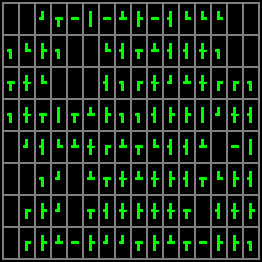
\includegraphics[scale=0.75]{\CURPATH/shuffled.png}
\caption{Разобранная головоломка}
\end{figure}

\dots и собранная:

\begin{figure}[H]
\label{fig:pipe_solved}
\centering
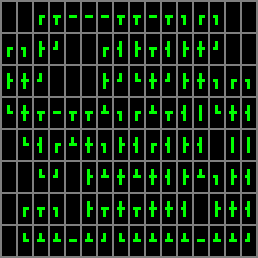
\includegraphics[scale=0.75]{\CURPATH/solved.png}
\caption{Собранная головоломка}
\end{figure}

Попробуем найти способ собрать её.

\subsubsection{Создание}

В начале, нужно её создать.
Вот простая идея.
Возьем массив ячеек 8*16.
Каждая ячейка может содержать какой-то тип блока.
Между ячейками есть стыки:

\input{\CURPATH/pipe_gen.tex}

Синие линии это горизонтальные стыки, красные линии это вертикальные стыки.
Мы просто случайно выставляем каждый стык в 0/false (отсутствует) или 1/true (присутствует).

После этого, теперь легко найти тип каждой ячейки.
А это:

\newcommand{\HeaderColor}{\cellcolor{blue!25}}
\begin{center}
\begin{longtable}{ | l | l | l | l | }
\hline
\HeaderColor стыки & \HeaderColor наше внутреннее название & \HeaderColor угол & \HeaderColor символ \\
\hline
0	&type 0		&	0$^{\circ}$	& (пробел)	\\
2	&type 2a	&	0$^{\circ}$	& \pmboxdrawuni{2503} \\ % ┃
2	&type 2a	&	90$^{\circ}$	& \pmboxdrawuni{2501} \\ % ━
2	&type 2b	&	0$^{\circ}$	& \pmboxdrawuni{250F} \\ % ┏
2	&type 2b	&	90$^{\circ}$	& \pmboxdrawuni{2513} \\ % ┓
2	&type 2b	&	180$^{\circ}$	& \pmboxdrawuni{251B} \\ % ┛
2	&type 2b	&	270$^{\circ}$	& \pmboxdrawuni{2517} \\ % ┗
3	&type 3		&	0$^{\circ}$	& \pmboxdrawuni{2523} \\ % ┣
3 	&type 3		&	90$^{\circ}$	& \pmboxdrawuni{2533} \\ % ┳
3	&type 3		&	180$^{\circ}$	& \pmboxdrawuni{252B} \\ % ┫
3	&type 3		&	270$^{\circ}$	& \pmboxdrawuni{253B} \\ % ┻
4	&type 4		&	0$^{\circ}$	& \pmboxdrawuni{254B} \\ % ╋
\hline
\end{longtable}
\end{center}

\textit{Висящие} стыки могут присутствовать на первой стадии (т.е., ячейки только с одним стыком), но они удалются
рекурсивно, и эти ячейки преобразуются в пустые ячейки.
Так что, в самом конце, все ячейки имеют минимум 2 стыка, и вся эта сантехническая система не имеет связей с внешним миром ---
я надеюсь, из-за этого станет немного проще.

Исходник генератора на Си здесь: \url{.../pipe/generator}.
Все вертикальные стыки хранятся в глобальном массиве \textit{hjoints[]} и вертикальные в \textit{vjoints[]}.

Программа на Си генерирует ANSI-раскрашенный вывод, как это было показано выше
(\ref{fig:pipe_shuffled}, \ref{fig:pipe_solved}) плюс массив типов для каждой ячейки, но без информации об углах:

\begin{lstlisting}[label=init_cells]
[
["0", "0", "2b", "3", "2a", "2a", "2a", "3", "3", "2a", "3", "2b", "2b", "2b", "0", "0"],
["2b", "2b", "3", "2b", "0", "0", "2b", "3", "3", "3", "3", "3", "4", "2b", "0", "0"],
["3", "4", "2b", "0", "0", "0", "3", "2b", "2b", "4", "2b", "3", "4", "2b", "2b", "2b"],
["2b", "4", "3", "2a", "3", "3", "3", "2b", "2b", "3", "3", "3", "2a", "2b", "4", "3"],
["0", "2b", "3", "2b", "3", "4", "2b", "3", "3", "2b", "3", "3", "3", "0", "2a", "2a"],
["0", "0", "2b", "2b", "0", "3", "3", "4", "3", "4", "3", "3", "3", "2b", "3", "3"],
["0", "2b", "3", "2b", "0", "3", "3", "4", "3", "4", "4", "3", "0", "3", "4", "3"],
["0", "2b", "3", "3", "2a", "3", "2b", "2b", "3", "3", "3", "3", "2a", "3", "3", "2b"],
]
\end{lstlisting}

\subsubsection{Решение}

Прежде всего, мы будем работать с массивом ячеек 8*16, где каждый элемент имеет 4 бита:
``T'' (top/верх),
``B'' (bottom/низ),
``L'' (left/лево),
``R'' (right/право).
Каждый бит представляет собой половину стыка.

\input{\CURPATH/pipe_solve.tex}

Теперь определяем массив для каждого из четырех полустыков + информация об угле:

\begin{lstlisting}
HEIGHT=8
WIDTH=16

# if T/B/R/L is Bool instead of Int, Z3 solver will work faster
T=[[Bool('cell_%d_%d_top' % (r, c)) for c in range(WIDTH)] for r in range(HEIGHT)]
B=[[Bool('cell_%d_%d_bottom' % (r, c)) for c in range(WIDTH)] for r in range(HEIGHT)]
R=[[Bool('cell_%d_%d_right' % (r, c)) for c in range(WIDTH)] for r in range(HEIGHT)]
L=[[Bool('cell_%d_%d_left' % (r, c)) for c in range(WIDTH)] for r in range(HEIGHT)]
A=[[Int('cell_%d_%d_angle' % (r, c)) for c in range(WIDTH)] for r in range(HEIGHT)]
\end{lstlisting}

Мы знаем, что если каждый из полустыков присутствует, ответный полустык также должен присутствовать, и наоборот. 
Определяем всё это используя эти констрайнты:

\begin{lstlisting}
# shorthand variables for True and False:
t=True
f=False

# "top" of each cell must be equal to "bottom" of the cell above
# "bottom" of each cell must be equal to "top" of the cell below
# "left" of each cell must be equal to "right" of the cell at left
# "right" of each cell must be equal to "left" of the cell at right
for r in range(HEIGHT):
    for c in range(WIDTH):
        if r!=0:
            s.add(T[r][c]==B[r-1][c])
        if r!=HEIGHT-1:
            s.add(B[r][c]==T[r+1][c])
        if c!=0:
            s.add(L[r][c]==R[r][c-1])
        if c!=WIDTH-1:
            s.add(R[r][c]==L[r][c+1])

# "left" of each cell of first column shouldn't have any connection
# so is "right" of each cell of the last column
for r in range(HEIGHT):
    s.add(L[r][0]==f)
    s.add(R[r][WIDTH-1]==f)

# "top" of each cell of the first row shouldn't have any connection
# so is "bottom" of each cell of the last row
for c in range(WIDTH):
    s.add(T[0][c]==f)
    s.add(B[HEIGHT-1][c]==f)
\end{lstlisting}

Теперь перебираем все ячейки в изначальном массиве (\ref{init_cells}).
Первые две ячейки здесь пустые. И третья имеет тип ``2b''.
Это ``\pmboxdrawuni{250F}'' % ┏
и его можно ориентировать четырьмя разными способами.
И если её угол это 0$^{\circ}$, верхний и правый полустыки присутствуют, остальные отсутствуют.
Если он имеет угол 90$^{\circ}$, он выглядит как 
``\pmboxdrawuni{2513}'', % ┓
и верхник и левый полустыки присутствуют, остальные отсутствуют.

На обычном русском языке: ``если ячейка этого типа имеет угол 0$^{\circ}$, вот эти полустыки должны присутствовать \textbf{ИЛИ}
если она имеет угол 90$^{\circ}$, эти полустыки должны присутствовать, \textbf{ИЛИ}, итд, итд.''

Точно также, мы определяем эти правила для всех типов и всех возможных углов:

\begin{lstlisting}
for r in range(HEIGHT):
    for c in range(WIDTH):
        ty=cells_type[r][c]

        if ty=="0":
            s.add(A[r][c]==f)
            s.add(T[r][c]==f, B[r][c]==f, L[r][c]==f, R[r][c]==f)

        if ty=="2a":
            s.add(Or(And(A[r][c]==0, L[r][c]==f, R[r][c]==f, T[r][c]==t, B[r][c]==t),   # §\pmboxdrawuni{2503}§
                    And(A[r][c]==90, L[r][c]==t, R[r][c]==t, T[r][c]==f, B[r][c]==f)))  # §\pmboxdrawuni{2501}§

        if ty=="2b":
            s.add(Or(And(A[r][c]==0, L[r][c]==f, R[r][c]==t, T[r][c]==f, B[r][c]==t),   # §\pmboxdrawuni{250F}§
                    And(A[r][c]==90, L[r][c]==t, R[r][c]==f, T[r][c]==f, B[r][c]==t),   # §\pmboxdrawuni{2513}§
                    And(A[r][c]==180, L[r][c]==t, R[r][c]==f, T[r][c]==t, B[r][c]==f),  # §\pmboxdrawuni{251B}§
                    And(A[r][c]==270, L[r][c]==f, R[r][c]==t, T[r][c]==t, B[r][c]==f))) # §\pmboxdrawuni{2517}§
	
        if ty=="3":
            s.add(Or(And(A[r][c]==0, L[r][c]==f, R[r][c]==t, T[r][c]==t, B[r][c]==t),   # §\pmboxdrawuni{2523}§
                    And(A[r][c]==90, L[r][c]==t, R[r][c]==t, T[r][c]==f, B[r][c]==t),   # §\pmboxdrawuni{2533}§
                    And(A[r][c]==180, L[r][c]==t, R[r][c]==f, T[r][c]==t, B[r][c]==t),  # §\pmboxdrawuni{252B}§
                    And(A[r][c]==270, L[r][c]==t, R[r][c]==t, T[r][c]==t, B[r][c]==f))) # §\pmboxdrawuni{253B}§

        if ty=="4":
            s.add(A[r][c]==0)
            s.add(T[r][c]==t, B[r][c]==t, L[r][c]==t, R[r][c]==t) # §\pmboxdrawuni{254B}§
\end{lstlisting}

Полный исходник здесь: \url{.../solver/solve_pipe_puzzle1.py}.

Получается такой результат (выводит угол для каждой ячейки и (псевдо)графическое представление):

\begin{figure}[H]
\centering
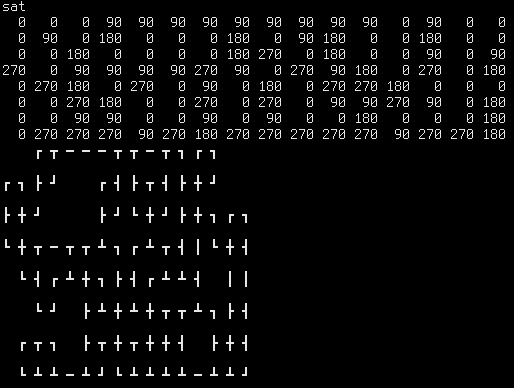
\includegraphics[scale=0.75]{\CURPATH/solver/solver.png}
\caption{Вывод скрипта солвера}
\end{figure}

Это работает $\approx 4$ секунды на моем старом и медленном Intel Atom N455 1.66GHz.
Быстро ли это? Не знаю, но снова вот что действительно круто, это то что мы понятия не имеем о какой-то математической
теории за всем этим, мы просто объявили ячейки, (полу-)стыки и определили отношения между ними.

Теперь следующий вопрос это, сколько здесь возможных решений?
Используя раннее описанный метод (\ref{SMTEnumerate}), я немного изменил скрипт солвера
\footnote{\url{.../solver/solve_pipe_puzzle2.py}} и солвер
сказал что возможно два решения.

Сравним их используя gvimdiff:

\begin{figure}[H]
\centering
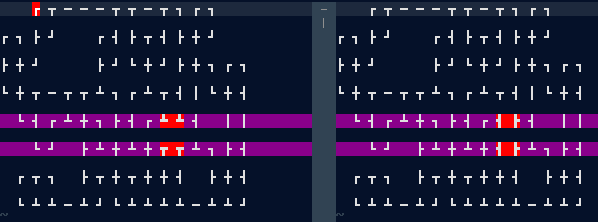
\includegraphics[scale=0.75]{\CURPATH/solver/diff.png}
\caption{Вывод gvimdiff (извините за мой красный курсор в левой части в левом верхнем углу)}
\end{figure}

4 ячейки в середине могут быть ориентированы по-разному.
Видимо, другие головоломки могут также выдавать разные результаты.

P.S.
\textit{Полу-стык} определен как булевый тип.
Но на самом деле, первая версия солвера была написана используя целочисленный тип для полу-стыков,
и 0 использовалось для False и 1 для True.
Я так сделал, потому что хотел более компактный исходный код, без использования длинных слов как ``False'' и ``True''.
И это работало, но медленнее. Вероятно, Z3 работает с булевыми типами быстрее? Лучше?
Так или иначе, я пишу это чтобы отметить, что, если нужно, целочисленный тип можно использовать вместо булевого.


\section{Развлекательная математика и головоломки}

\input{puzzles/sudoku/main_RU}
\input{puzzles/zebra/main_RU}
\input{puzzles/pipe/main_RU}
\input{puzzles/rubik2/failed_SMT/main_RU}
\input{puzzles/rubik2/SAT/main_RU}
\input{puzzles/rubik3/one_face_SMT/main_RU}
%\input{puzzles/numberlink/main_RU}
%\input{puzzles/two_parks_RU}
\input{puzzles/alphametics/main_RU}
%\input{puzzles/2015_AIME_II_Problems_12_RU}
%\input{puzzles/fred/main_RU}
%\input{puzzles/MC/main_RU}
%\input{puzzles/coin_flip/main_RU}
%\input{puzzles/Mock_AIME_2_2006-2007_Problem_8_RU}
%\input{puzzles/2012_AIME_I_Problems_1_RU}
%\input{puzzles/keypad_RU}


\section{Развлекательная математика и головоломки}

\input{puzzles/sudoku/main_RU}
\input{puzzles/zebra/main_RU}
\input{puzzles/pipe/main_RU}
\input{puzzles/rubik2/failed_SMT/main_RU}
\input{puzzles/rubik2/SAT/main_RU}
\input{puzzles/rubik3/one_face_SMT/main_RU}
%\input{puzzles/numberlink/main_RU}
%\input{puzzles/two_parks_RU}
\input{puzzles/alphametics/main_RU}
%\input{puzzles/2015_AIME_II_Problems_12_RU}
%\input{puzzles/fred/main_RU}
%\input{puzzles/MC/main_RU}
%\input{puzzles/coin_flip/main_RU}
%\input{puzzles/Mock_AIME_2_2006-2007_Problem_8_RU}
%\input{puzzles/2012_AIME_I_Problems_1_RU}
%\input{puzzles/keypad_RU}


\section{Развлекательная математика и головоломки}

\input{puzzles/sudoku/main_RU}
\input{puzzles/zebra/main_RU}
\input{puzzles/pipe/main_RU}
\input{puzzles/rubik2/failed_SMT/main_RU}
\input{puzzles/rubik2/SAT/main_RU}
\input{puzzles/rubik3/one_face_SMT/main_RU}
%\input{puzzles/numberlink/main_RU}
%\input{puzzles/two_parks_RU}
\input{puzzles/alphametics/main_RU}
%\input{puzzles/2015_AIME_II_Problems_12_RU}
%\input{puzzles/fred/main_RU}
%\input{puzzles/MC/main_RU}
%\input{puzzles/coin_flip/main_RU}
%\input{puzzles/Mock_AIME_2_2006-2007_Problem_8_RU}
%\input{puzzles/2012_AIME_I_Problems_1_RU}
%\input{puzzles/keypad_RU}


%\section{Развлекательная математика и головоломки}

\input{puzzles/sudoku/main_RU}
\input{puzzles/zebra/main_RU}
\input{puzzles/pipe/main_RU}
\input{puzzles/rubik2/failed_SMT/main_RU}
\input{puzzles/rubik2/SAT/main_RU}
\input{puzzles/rubik3/one_face_SMT/main_RU}
%\input{puzzles/numberlink/main_RU}
%\input{puzzles/two_parks_RU}
\input{puzzles/alphametics/main_RU}
%\input{puzzles/2015_AIME_II_Problems_12_RU}
%\input{puzzles/fred/main_RU}
%\input{puzzles/MC/main_RU}
%\input{puzzles/coin_flip/main_RU}
%\input{puzzles/Mock_AIME_2_2006-2007_Problem_8_RU}
%\input{puzzles/2012_AIME_I_Problems_1_RU}
%\input{puzzles/keypad_RU}


%\input{puzzles/two_parks_RU}
\subsection{Альфаметика}

Согласно Дональду Кнуту, термин ``Альфаметика'' был придуман Дж. Эйч. Аш. Хантером.
Это головоломка: какие десятичные цифры в пределах 0..9 нужно присвоить каждой букве, чтобы это уравнение было справедливо?

\begin{lstlisting}
  SEND
+ MORE
 -----
 MONEY
\end{lstlisting}

Для Z3 это легко:

\lstinputlisting{puzzles/alphametics/alpha.py}

Вывод:

\begin{lstlisting}
sat
[E, = 5,
 S, = 9,
 M, = 1,
 N, = 6,
 D, = 7,
 R, = 8,
 O, = 0,
 Y = 2]
\end{lstlisting}

Вот еще одна, из \ac{TAOCP} том IV (\url{http://www-cs-faculty.stanford.edu/~uno/fasc2b.ps.gz}):

\lstinputlisting{puzzles/alphametics/alpha2.py}

\begin{lstlisting}
sat
[L, = 6,
 S, = 7,
 N, = 2,
 T, = 1,
 I, = 5,
 V = 3,
 A, = 8,
 R, = 9,
 O, = 4,
 TRIO = 1954,
 SONATA, = 742818,
 VIOLA, = 35468,
 VIOLIN, = 354652]
\end{lstlisting}

% TODO URL
Эту головоломку я нашел в примерах pySMT:

\lstinputlisting{puzzles/alphametics/alpha3.py}

\begin{lstlisting}
sat
[D = 5, R = 4, O = 3, E = 8, L = 6, W = 7, H = 2]
\end{lstlisting}

%%% 

Это упражнение Q209 из
[Companion to the Papers of Donald Knuth]\footnote{\url{http://www-cs-faculty.stanford.edu/~knuth/cp.html}}.

\begin{lstlisting}
 KNIFE
  FORK
 SPOON
  SOUP
------
SUPPER
\end{lstlisting}

В целях упрощения, я добавил ф-цию (list\_to\_expr()):

\lstinputlisting{puzzles/alphametics/alpha4.py}

\begin{lstlisting}
sat
[K = 7,
 N = 4,
 R = 9,
 I = 1,
 E = 6,
 S = 0,
 O = 3,
 F = 5,
 U = 8,
 P = 2,
 SUPPER = 82269,
 SOUP = 382,
 SPOON = 2334,
 FORK = 5397,
 KNIFE = 74156]
\end{lstlisting}

S это 0, так что значение SUPPER начинается с (убранного) нуля. Скажем так, нам это не нравится.
Добавим это, чтобы это исправить:

\begin{lstlisting}
s.add(S!=0)
\end{lstlisting}

\begin{lstlisting}
sat
[K = 8,
 N = 4,
 R = 3,
 I = 7,
 E = 6,
 S = 1,
 O = 9,
 F = 2,
 U = 0,
 P = 5,
 SUPPER = 105563,
 SOUP = 1905,
 SPOON = 15994,
 FORK = 2938,
 KNIFE = 84726]
\end{lstlisting}

\paragraph{Создание своей собственной головоломки}

Вот проблема: есть только 10 букв, но как их выбрать из числа слов?
Мы можем использовать Z3 для этого:

\lstinputlisting{puzzles/alphametics/gen.py}

Это первая сгенерированная головоломка:

\begin{lstlisting}
sat
EGGS
JELLY
LUNCH
C 5
E 6
G 3
H 7
J 0
L 1
N 4
S 8
U 2
Y 9
\end{lstlisting}

Что если мы хотим, чтобы слово ``CAKE'' присутствовало в числе ``слагаемых''?

Добавим это:

\begin{lstlisting}
s.add(word_used[words.index('CAKE')])
\end{lstlisting}

\begin{lstlisting}
sat
CAKE
TEA
LUNCH
A 8
C 3
E 1
H 9
J 6
K 2
L 0
N 5
T 7
U 4
\end{lstlisting}

Добавим это:

\begin{lstlisting}
s.add(word_used[words.index('EGGS')])
\end{lstlisting}

Теперь оно может найти пару к EGGS:

\begin{lstlisting}
sat
EGGS
HONEY
LUNCH
C 6
E 7
G 9
H 4
L 5
N 8
O 2
S 3
U 0
Y 1
\end{lstlisting}

\paragraph{Файлы}

\url{https://github.com/DennisYurichev/...}




%\input{puzzles/2015_AIME_II_Problems_12_RU}
%\section{Развлекательная математика и головоломки}

\input{puzzles/sudoku/main_RU}
\input{puzzles/zebra/main_RU}
\input{puzzles/pipe/main_RU}
\input{puzzles/rubik2/failed_SMT/main_RU}
\input{puzzles/rubik2/SAT/main_RU}
\input{puzzles/rubik3/one_face_SMT/main_RU}
%\input{puzzles/numberlink/main_RU}
%\input{puzzles/two_parks_RU}
\input{puzzles/alphametics/main_RU}
%\input{puzzles/2015_AIME_II_Problems_12_RU}
%\input{puzzles/fred/main_RU}
%\input{puzzles/MC/main_RU}
%\input{puzzles/coin_flip/main_RU}
%\input{puzzles/Mock_AIME_2_2006-2007_Problem_8_RU}
%\input{puzzles/2012_AIME_I_Problems_1_RU}
%\input{puzzles/keypad_RU}


%\section{Развлекательная математика и головоломки}

\input{puzzles/sudoku/main_RU}
\input{puzzles/zebra/main_RU}
\input{puzzles/pipe/main_RU}
\input{puzzles/rubik2/failed_SMT/main_RU}
\input{puzzles/rubik2/SAT/main_RU}
\input{puzzles/rubik3/one_face_SMT/main_RU}
%\input{puzzles/numberlink/main_RU}
%\input{puzzles/two_parks_RU}
\input{puzzles/alphametics/main_RU}
%\input{puzzles/2015_AIME_II_Problems_12_RU}
%\input{puzzles/fred/main_RU}
%\input{puzzles/MC/main_RU}
%\input{puzzles/coin_flip/main_RU}
%\input{puzzles/Mock_AIME_2_2006-2007_Problem_8_RU}
%\input{puzzles/2012_AIME_I_Problems_1_RU}
%\input{puzzles/keypad_RU}


%\section{Развлекательная математика и головоломки}

\input{puzzles/sudoku/main_RU}
\input{puzzles/zebra/main_RU}
\input{puzzles/pipe/main_RU}
\input{puzzles/rubik2/failed_SMT/main_RU}
\input{puzzles/rubik2/SAT/main_RU}
\input{puzzles/rubik3/one_face_SMT/main_RU}
%\input{puzzles/numberlink/main_RU}
%\input{puzzles/two_parks_RU}
\input{puzzles/alphametics/main_RU}
%\input{puzzles/2015_AIME_II_Problems_12_RU}
%\input{puzzles/fred/main_RU}
%\input{puzzles/MC/main_RU}
%\input{puzzles/coin_flip/main_RU}
%\input{puzzles/Mock_AIME_2_2006-2007_Problem_8_RU}
%\input{puzzles/2012_AIME_I_Problems_1_RU}
%\input{puzzles/keypad_RU}


%\input{puzzles/Mock_AIME_2_2006-2007_Problem_8_RU}
%\input{puzzles/2012_AIME_I_Problems_1_RU}
%\input{puzzles/keypad_RU}


%\section{Развлекательная математика и головоломки}

\subsection{Судоку}

Головоломка Судоку это решетка 9*9, некоторые ячейки заполнены значениями, некоторые пустые:

% copypasted from http://www.texample.net/tikz/examples/sudoku/
\newcounter{row}
\newcounter{col}

\newcommand\setrow[9]{
  \setcounter{col}{1}
  \foreach \n in {#1, #2, #3, #4, #5, #6, #7, #8, #9} {
    \edef\x{\value{col} - 0.5}
    \edef\y{9.5 - \value{row}}
    \node[anchor=center] at (\x, \y) {\n};
    \stepcounter{col}
  }
  \stepcounter{row}
}

\begin{center}
\begin{tikzpicture}[scale=.7]
  \begin{scope}
    \draw (0, 0) grid (9, 9);
    \draw[very thick, scale=3] (0, 0) grid (3, 3);

    \setcounter{row}{1}
    \setrow { }{ }{5}  {3}{ }{ }  { }{ }{ }
    \setrow {8}{ }{ }  { }{ }{ }  { }{2}{ }
    \setrow { }{7}{ }  { }{1}{ }  {5}{ }{ }

    \setrow {4}{ }{ }  { }{ }{5}  {3}{ }{ }
    \setrow { }{1}{ }  { }{7}{ }  { }{ }{6}
    \setrow { }{ }{3}  {2}{ }{ }  { }{8}{ }

    \setrow { }{6}{ }  {5}{ }{ }  { }{ }{9}
    \setrow { }{ }{4}  { }{ }{ }  { }{3}{ }
    \setrow { }{ }{ }  { }{ }{9}  {7}{ }{ }

    \node[anchor=center] at (4.5, -0.5) {Нерешенная Судоку};
  \end{scope}
\end{tikzpicture}
\end{center}

Числа в каждом ряду должны быть уникальными, т.е., каждый ряд должен содержать 9 чисел в пределах 1..9 без повторений.
Та же история и для каждого столбца и каждого квадрата 3*3.

Головоломка представляет собой хороший кандидат, на котором можно попробовать \ac{SMT}-солвер, потому что это,
в общем-то, просто нерешенная система уравнений.

\input{puzzles/sudoku/1/main_RU}
%\input{puzzles/sudoku/GT/main_RU}
%\input{puzzles/sudoku/killer/main_RU}
\input{puzzles/sudoku/KLEE/main_RU}
\input{puzzles/sudoku/SAT/main_RU}


\subsection{Головоломка зебры (\ac{AKA} Загадка Эйнштейна)}

\input{puzzles/zebra/SMT/main_RU}
\input{puzzles/zebra/KLEE/main_RU}
\input{puzzles/zebra/SAT/main_RU}


\subsection{Решение головоломки ``трубы'' используя Z3 SMT-солвер}

\renewcommand{\CURPATH}{puzzles/pipe}

Головоломка ``трубы'' это популярная головоломка (просто погуглите ``pipe puzzle'' и посмотрите на картинки).

Вот как выглядит головоломка в разобранном виде:

\begin{figure}[H]
\label{fig:pipe_shuffled}
\centering
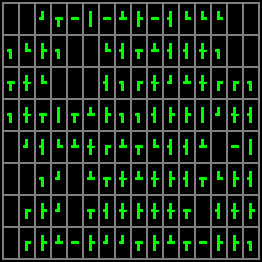
\includegraphics[scale=0.75]{\CURPATH/shuffled.png}
\caption{Разобранная головоломка}
\end{figure}

\dots и собранная:

\begin{figure}[H]
\label{fig:pipe_solved}
\centering
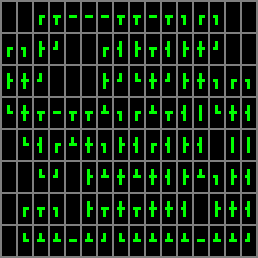
\includegraphics[scale=0.75]{\CURPATH/solved.png}
\caption{Собранная головоломка}
\end{figure}

Попробуем найти способ собрать её.

\subsubsection{Создание}

В начале, нужно её создать.
Вот простая идея.
Возьем массив ячеек 8*16.
Каждая ячейка может содержать какой-то тип блока.
Между ячейками есть стыки:

\input{\CURPATH/pipe_gen.tex}

Синие линии это горизонтальные стыки, красные линии это вертикальные стыки.
Мы просто случайно выставляем каждый стык в 0/false (отсутствует) или 1/true (присутствует).

После этого, теперь легко найти тип каждой ячейки.
А это:

\newcommand{\HeaderColor}{\cellcolor{blue!25}}
\begin{center}
\begin{longtable}{ | l | l | l | l | }
\hline
\HeaderColor стыки & \HeaderColor наше внутреннее название & \HeaderColor угол & \HeaderColor символ \\
\hline
0	&type 0		&	0$^{\circ}$	& (пробел)	\\
2	&type 2a	&	0$^{\circ}$	& \pmboxdrawuni{2503} \\ % ┃
2	&type 2a	&	90$^{\circ}$	& \pmboxdrawuni{2501} \\ % ━
2	&type 2b	&	0$^{\circ}$	& \pmboxdrawuni{250F} \\ % ┏
2	&type 2b	&	90$^{\circ}$	& \pmboxdrawuni{2513} \\ % ┓
2	&type 2b	&	180$^{\circ}$	& \pmboxdrawuni{251B} \\ % ┛
2	&type 2b	&	270$^{\circ}$	& \pmboxdrawuni{2517} \\ % ┗
3	&type 3		&	0$^{\circ}$	& \pmboxdrawuni{2523} \\ % ┣
3 	&type 3		&	90$^{\circ}$	& \pmboxdrawuni{2533} \\ % ┳
3	&type 3		&	180$^{\circ}$	& \pmboxdrawuni{252B} \\ % ┫
3	&type 3		&	270$^{\circ}$	& \pmboxdrawuni{253B} \\ % ┻
4	&type 4		&	0$^{\circ}$	& \pmboxdrawuni{254B} \\ % ╋
\hline
\end{longtable}
\end{center}

\textit{Висящие} стыки могут присутствовать на первой стадии (т.е., ячейки только с одним стыком), но они удалются
рекурсивно, и эти ячейки преобразуются в пустые ячейки.
Так что, в самом конце, все ячейки имеют минимум 2 стыка, и вся эта сантехническая система не имеет связей с внешним миром ---
я надеюсь, из-за этого станет немного проще.

Исходник генератора на Си здесь: \url{.../pipe/generator}.
Все вертикальные стыки хранятся в глобальном массиве \textit{hjoints[]} и вертикальные в \textit{vjoints[]}.

Программа на Си генерирует ANSI-раскрашенный вывод, как это было показано выше
(\ref{fig:pipe_shuffled}, \ref{fig:pipe_solved}) плюс массив типов для каждой ячейки, но без информации об углах:

\begin{lstlisting}[label=init_cells]
[
["0", "0", "2b", "3", "2a", "2a", "2a", "3", "3", "2a", "3", "2b", "2b", "2b", "0", "0"],
["2b", "2b", "3", "2b", "0", "0", "2b", "3", "3", "3", "3", "3", "4", "2b", "0", "0"],
["3", "4", "2b", "0", "0", "0", "3", "2b", "2b", "4", "2b", "3", "4", "2b", "2b", "2b"],
["2b", "4", "3", "2a", "3", "3", "3", "2b", "2b", "3", "3", "3", "2a", "2b", "4", "3"],
["0", "2b", "3", "2b", "3", "4", "2b", "3", "3", "2b", "3", "3", "3", "0", "2a", "2a"],
["0", "0", "2b", "2b", "0", "3", "3", "4", "3", "4", "3", "3", "3", "2b", "3", "3"],
["0", "2b", "3", "2b", "0", "3", "3", "4", "3", "4", "4", "3", "0", "3", "4", "3"],
["0", "2b", "3", "3", "2a", "3", "2b", "2b", "3", "3", "3", "3", "2a", "3", "3", "2b"],
]
\end{lstlisting}

\subsubsection{Решение}

Прежде всего, мы будем работать с массивом ячеек 8*16, где каждый элемент имеет 4 бита:
``T'' (top/верх),
``B'' (bottom/низ),
``L'' (left/лево),
``R'' (right/право).
Каждый бит представляет собой половину стыка.

\input{\CURPATH/pipe_solve.tex}

Теперь определяем массив для каждого из четырех полустыков + информация об угле:

\begin{lstlisting}
HEIGHT=8
WIDTH=16

# if T/B/R/L is Bool instead of Int, Z3 solver will work faster
T=[[Bool('cell_%d_%d_top' % (r, c)) for c in range(WIDTH)] for r in range(HEIGHT)]
B=[[Bool('cell_%d_%d_bottom' % (r, c)) for c in range(WIDTH)] for r in range(HEIGHT)]
R=[[Bool('cell_%d_%d_right' % (r, c)) for c in range(WIDTH)] for r in range(HEIGHT)]
L=[[Bool('cell_%d_%d_left' % (r, c)) for c in range(WIDTH)] for r in range(HEIGHT)]
A=[[Int('cell_%d_%d_angle' % (r, c)) for c in range(WIDTH)] for r in range(HEIGHT)]
\end{lstlisting}

Мы знаем, что если каждый из полустыков присутствует, ответный полустык также должен присутствовать, и наоборот. 
Определяем всё это используя эти констрайнты:

\begin{lstlisting}
# shorthand variables for True and False:
t=True
f=False

# "top" of each cell must be equal to "bottom" of the cell above
# "bottom" of each cell must be equal to "top" of the cell below
# "left" of each cell must be equal to "right" of the cell at left
# "right" of each cell must be equal to "left" of the cell at right
for r in range(HEIGHT):
    for c in range(WIDTH):
        if r!=0:
            s.add(T[r][c]==B[r-1][c])
        if r!=HEIGHT-1:
            s.add(B[r][c]==T[r+1][c])
        if c!=0:
            s.add(L[r][c]==R[r][c-1])
        if c!=WIDTH-1:
            s.add(R[r][c]==L[r][c+1])

# "left" of each cell of first column shouldn't have any connection
# so is "right" of each cell of the last column
for r in range(HEIGHT):
    s.add(L[r][0]==f)
    s.add(R[r][WIDTH-1]==f)

# "top" of each cell of the first row shouldn't have any connection
# so is "bottom" of each cell of the last row
for c in range(WIDTH):
    s.add(T[0][c]==f)
    s.add(B[HEIGHT-1][c]==f)
\end{lstlisting}

Теперь перебираем все ячейки в изначальном массиве (\ref{init_cells}).
Первые две ячейки здесь пустые. И третья имеет тип ``2b''.
Это ``\pmboxdrawuni{250F}'' % ┏
и его можно ориентировать четырьмя разными способами.
И если её угол это 0$^{\circ}$, верхний и правый полустыки присутствуют, остальные отсутствуют.
Если он имеет угол 90$^{\circ}$, он выглядит как 
``\pmboxdrawuni{2513}'', % ┓
и верхник и левый полустыки присутствуют, остальные отсутствуют.

На обычном русском языке: ``если ячейка этого типа имеет угол 0$^{\circ}$, вот эти полустыки должны присутствовать \textbf{ИЛИ}
если она имеет угол 90$^{\circ}$, эти полустыки должны присутствовать, \textbf{ИЛИ}, итд, итд.''

Точно также, мы определяем эти правила для всех типов и всех возможных углов:

\begin{lstlisting}
for r in range(HEIGHT):
    for c in range(WIDTH):
        ty=cells_type[r][c]

        if ty=="0":
            s.add(A[r][c]==f)
            s.add(T[r][c]==f, B[r][c]==f, L[r][c]==f, R[r][c]==f)

        if ty=="2a":
            s.add(Or(And(A[r][c]==0, L[r][c]==f, R[r][c]==f, T[r][c]==t, B[r][c]==t),   # §\pmboxdrawuni{2503}§
                    And(A[r][c]==90, L[r][c]==t, R[r][c]==t, T[r][c]==f, B[r][c]==f)))  # §\pmboxdrawuni{2501}§

        if ty=="2b":
            s.add(Or(And(A[r][c]==0, L[r][c]==f, R[r][c]==t, T[r][c]==f, B[r][c]==t),   # §\pmboxdrawuni{250F}§
                    And(A[r][c]==90, L[r][c]==t, R[r][c]==f, T[r][c]==f, B[r][c]==t),   # §\pmboxdrawuni{2513}§
                    And(A[r][c]==180, L[r][c]==t, R[r][c]==f, T[r][c]==t, B[r][c]==f),  # §\pmboxdrawuni{251B}§
                    And(A[r][c]==270, L[r][c]==f, R[r][c]==t, T[r][c]==t, B[r][c]==f))) # §\pmboxdrawuni{2517}§
	
        if ty=="3":
            s.add(Or(And(A[r][c]==0, L[r][c]==f, R[r][c]==t, T[r][c]==t, B[r][c]==t),   # §\pmboxdrawuni{2523}§
                    And(A[r][c]==90, L[r][c]==t, R[r][c]==t, T[r][c]==f, B[r][c]==t),   # §\pmboxdrawuni{2533}§
                    And(A[r][c]==180, L[r][c]==t, R[r][c]==f, T[r][c]==t, B[r][c]==t),  # §\pmboxdrawuni{252B}§
                    And(A[r][c]==270, L[r][c]==t, R[r][c]==t, T[r][c]==t, B[r][c]==f))) # §\pmboxdrawuni{253B}§

        if ty=="4":
            s.add(A[r][c]==0)
            s.add(T[r][c]==t, B[r][c]==t, L[r][c]==t, R[r][c]==t) # §\pmboxdrawuni{254B}§
\end{lstlisting}

Полный исходник здесь: \url{.../solver/solve_pipe_puzzle1.py}.

Получается такой результат (выводит угол для каждой ячейки и (псевдо)графическое представление):

\begin{figure}[H]
\centering
\includegraphics[scale=0.75]{\CURPATH/solver/solver.png}
\caption{Вывод скрипта солвера}
\end{figure}

Это работает $\approx 4$ секунды на моем старом и медленном Intel Atom N455 1.66GHz.
Быстро ли это? Не знаю, но снова вот что действительно круто, это то что мы понятия не имеем о какой-то математической
теории за всем этим, мы просто объявили ячейки, (полу-)стыки и определили отношения между ними.

Теперь следующий вопрос это, сколько здесь возможных решений?
Используя раннее описанный метод (\ref{SMTEnumerate}), я немного изменил скрипт солвера
\footnote{\url{.../solver/solve_pipe_puzzle2.py}} и солвер
сказал что возможно два решения.

Сравним их используя gvimdiff:

\begin{figure}[H]
\centering
\includegraphics[scale=0.75]{\CURPATH/solver/diff.png}
\caption{Вывод gvimdiff (извините за мой красный курсор в левой части в левом верхнем углу)}
\end{figure}

4 ячейки в середине могут быть ориентированы по-разному.
Видимо, другие головоломки могут также выдавать разные результаты.

P.S.
\textit{Полу-стык} определен как булевый тип.
Но на самом деле, первая версия солвера была написана используя целочисленный тип для полу-стыков,
и 0 использовалось для False и 1 для True.
Я так сделал, потому что хотел более компактный исходный код, без использования длинных слов как ``False'' и ``True''.
И это работало, но медленнее. Вероятно, Z3 работает с булевыми типами быстрее? Лучше?
Так или иначе, я пишу это чтобы отметить, что, если нужно, целочисленный тип можно использовать вместо булевого.


\section{Развлекательная математика и головоломки}

\input{puzzles/sudoku/main_RU}
\input{puzzles/zebra/main_RU}
\input{puzzles/pipe/main_RU}
\input{puzzles/rubik2/failed_SMT/main_RU}
\input{puzzles/rubik2/SAT/main_RU}
\input{puzzles/rubik3/one_face_SMT/main_RU}
%\input{puzzles/numberlink/main_RU}
%\input{puzzles/two_parks_RU}
\input{puzzles/alphametics/main_RU}
%\input{puzzles/2015_AIME_II_Problems_12_RU}
%\input{puzzles/fred/main_RU}
%\input{puzzles/MC/main_RU}
%\input{puzzles/coin_flip/main_RU}
%\input{puzzles/Mock_AIME_2_2006-2007_Problem_8_RU}
%\input{puzzles/2012_AIME_I_Problems_1_RU}
%\input{puzzles/keypad_RU}


\section{Развлекательная математика и головоломки}

\input{puzzles/sudoku/main_RU}
\input{puzzles/zebra/main_RU}
\input{puzzles/pipe/main_RU}
\input{puzzles/rubik2/failed_SMT/main_RU}
\input{puzzles/rubik2/SAT/main_RU}
\input{puzzles/rubik3/one_face_SMT/main_RU}
%\input{puzzles/numberlink/main_RU}
%\input{puzzles/two_parks_RU}
\input{puzzles/alphametics/main_RU}
%\input{puzzles/2015_AIME_II_Problems_12_RU}
%\input{puzzles/fred/main_RU}
%\input{puzzles/MC/main_RU}
%\input{puzzles/coin_flip/main_RU}
%\input{puzzles/Mock_AIME_2_2006-2007_Problem_8_RU}
%\input{puzzles/2012_AIME_I_Problems_1_RU}
%\input{puzzles/keypad_RU}


\section{Развлекательная математика и головоломки}

\input{puzzles/sudoku/main_RU}
\input{puzzles/zebra/main_RU}
\input{puzzles/pipe/main_RU}
\input{puzzles/rubik2/failed_SMT/main_RU}
\input{puzzles/rubik2/SAT/main_RU}
\input{puzzles/rubik3/one_face_SMT/main_RU}
%\input{puzzles/numberlink/main_RU}
%\input{puzzles/two_parks_RU}
\input{puzzles/alphametics/main_RU}
%\input{puzzles/2015_AIME_II_Problems_12_RU}
%\input{puzzles/fred/main_RU}
%\input{puzzles/MC/main_RU}
%\input{puzzles/coin_flip/main_RU}
%\input{puzzles/Mock_AIME_2_2006-2007_Problem_8_RU}
%\input{puzzles/2012_AIME_I_Problems_1_RU}
%\input{puzzles/keypad_RU}


%\section{Развлекательная математика и головоломки}

\input{puzzles/sudoku/main_RU}
\input{puzzles/zebra/main_RU}
\input{puzzles/pipe/main_RU}
\input{puzzles/rubik2/failed_SMT/main_RU}
\input{puzzles/rubik2/SAT/main_RU}
\input{puzzles/rubik3/one_face_SMT/main_RU}
%\input{puzzles/numberlink/main_RU}
%\input{puzzles/two_parks_RU}
\input{puzzles/alphametics/main_RU}
%\input{puzzles/2015_AIME_II_Problems_12_RU}
%\input{puzzles/fred/main_RU}
%\input{puzzles/MC/main_RU}
%\input{puzzles/coin_flip/main_RU}
%\input{puzzles/Mock_AIME_2_2006-2007_Problem_8_RU}
%\input{puzzles/2012_AIME_I_Problems_1_RU}
%\input{puzzles/keypad_RU}


%\input{puzzles/two_parks_RU}
\subsection{Альфаметика}

Согласно Дональду Кнуту, термин ``Альфаметика'' был придуман Дж. Эйч. Аш. Хантером.
Это головоломка: какие десятичные цифры в пределах 0..9 нужно присвоить каждой букве, чтобы это уравнение было справедливо?

\begin{lstlisting}
  SEND
+ MORE
 -----
 MONEY
\end{lstlisting}

Для Z3 это легко:

\lstinputlisting{puzzles/alphametics/alpha.py}

Вывод:

\begin{lstlisting}
sat
[E, = 5,
 S, = 9,
 M, = 1,
 N, = 6,
 D, = 7,
 R, = 8,
 O, = 0,
 Y = 2]
\end{lstlisting}

Вот еще одна, из \ac{TAOCP} том IV (\url{http://www-cs-faculty.stanford.edu/~uno/fasc2b.ps.gz}):

\lstinputlisting{puzzles/alphametics/alpha2.py}

\begin{lstlisting}
sat
[L, = 6,
 S, = 7,
 N, = 2,
 T, = 1,
 I, = 5,
 V = 3,
 A, = 8,
 R, = 9,
 O, = 4,
 TRIO = 1954,
 SONATA, = 742818,
 VIOLA, = 35468,
 VIOLIN, = 354652]
\end{lstlisting}

% TODO URL
Эту головоломку я нашел в примерах pySMT:

\lstinputlisting{puzzles/alphametics/alpha3.py}

\begin{lstlisting}
sat
[D = 5, R = 4, O = 3, E = 8, L = 6, W = 7, H = 2]
\end{lstlisting}

%%% 

Это упражнение Q209 из
[Companion to the Papers of Donald Knuth]\footnote{\url{http://www-cs-faculty.stanford.edu/~knuth/cp.html}}.

\begin{lstlisting}
 KNIFE
  FORK
 SPOON
  SOUP
------
SUPPER
\end{lstlisting}

В целях упрощения, я добавил ф-цию (list\_to\_expr()):

\lstinputlisting{puzzles/alphametics/alpha4.py}

\begin{lstlisting}
sat
[K = 7,
 N = 4,
 R = 9,
 I = 1,
 E = 6,
 S = 0,
 O = 3,
 F = 5,
 U = 8,
 P = 2,
 SUPPER = 82269,
 SOUP = 382,
 SPOON = 2334,
 FORK = 5397,
 KNIFE = 74156]
\end{lstlisting}

S это 0, так что значение SUPPER начинается с (убранного) нуля. Скажем так, нам это не нравится.
Добавим это, чтобы это исправить:

\begin{lstlisting}
s.add(S!=0)
\end{lstlisting}

\begin{lstlisting}
sat
[K = 8,
 N = 4,
 R = 3,
 I = 7,
 E = 6,
 S = 1,
 O = 9,
 F = 2,
 U = 0,
 P = 5,
 SUPPER = 105563,
 SOUP = 1905,
 SPOON = 15994,
 FORK = 2938,
 KNIFE = 84726]
\end{lstlisting}

\paragraph{Создание своей собственной головоломки}

Вот проблема: есть только 10 букв, но как их выбрать из числа слов?
Мы можем использовать Z3 для этого:

\lstinputlisting{puzzles/alphametics/gen.py}

Это первая сгенерированная головоломка:

\begin{lstlisting}
sat
EGGS
JELLY
LUNCH
C 5
E 6
G 3
H 7
J 0
L 1
N 4
S 8
U 2
Y 9
\end{lstlisting}

Что если мы хотим, чтобы слово ``CAKE'' присутствовало в числе ``слагаемых''?

Добавим это:

\begin{lstlisting}
s.add(word_used[words.index('CAKE')])
\end{lstlisting}

\begin{lstlisting}
sat
CAKE
TEA
LUNCH
A 8
C 3
E 1
H 9
J 6
K 2
L 0
N 5
T 7
U 4
\end{lstlisting}

Добавим это:

\begin{lstlisting}
s.add(word_used[words.index('EGGS')])
\end{lstlisting}

Теперь оно может найти пару к EGGS:

\begin{lstlisting}
sat
EGGS
HONEY
LUNCH
C 6
E 7
G 9
H 4
L 5
N 8
O 2
S 3
U 0
Y 1
\end{lstlisting}

\paragraph{Файлы}

\url{https://github.com/DennisYurichev/...}




%\input{puzzles/2015_AIME_II_Problems_12_RU}
%\section{Развлекательная математика и головоломки}

\input{puzzles/sudoku/main_RU}
\input{puzzles/zebra/main_RU}
\input{puzzles/pipe/main_RU}
\input{puzzles/rubik2/failed_SMT/main_RU}
\input{puzzles/rubik2/SAT/main_RU}
\input{puzzles/rubik3/one_face_SMT/main_RU}
%\input{puzzles/numberlink/main_RU}
%\input{puzzles/two_parks_RU}
\input{puzzles/alphametics/main_RU}
%\input{puzzles/2015_AIME_II_Problems_12_RU}
%\input{puzzles/fred/main_RU}
%\input{puzzles/MC/main_RU}
%\input{puzzles/coin_flip/main_RU}
%\input{puzzles/Mock_AIME_2_2006-2007_Problem_8_RU}
%\input{puzzles/2012_AIME_I_Problems_1_RU}
%\input{puzzles/keypad_RU}


%\section{Развлекательная математика и головоломки}

\input{puzzles/sudoku/main_RU}
\input{puzzles/zebra/main_RU}
\input{puzzles/pipe/main_RU}
\input{puzzles/rubik2/failed_SMT/main_RU}
\input{puzzles/rubik2/SAT/main_RU}
\input{puzzles/rubik3/one_face_SMT/main_RU}
%\input{puzzles/numberlink/main_RU}
%\input{puzzles/two_parks_RU}
\input{puzzles/alphametics/main_RU}
%\input{puzzles/2015_AIME_II_Problems_12_RU}
%\input{puzzles/fred/main_RU}
%\input{puzzles/MC/main_RU}
%\input{puzzles/coin_flip/main_RU}
%\input{puzzles/Mock_AIME_2_2006-2007_Problem_8_RU}
%\input{puzzles/2012_AIME_I_Problems_1_RU}
%\input{puzzles/keypad_RU}


%\section{Развлекательная математика и головоломки}

\input{puzzles/sudoku/main_RU}
\input{puzzles/zebra/main_RU}
\input{puzzles/pipe/main_RU}
\input{puzzles/rubik2/failed_SMT/main_RU}
\input{puzzles/rubik2/SAT/main_RU}
\input{puzzles/rubik3/one_face_SMT/main_RU}
%\input{puzzles/numberlink/main_RU}
%\input{puzzles/two_parks_RU}
\input{puzzles/alphametics/main_RU}
%\input{puzzles/2015_AIME_II_Problems_12_RU}
%\input{puzzles/fred/main_RU}
%\input{puzzles/MC/main_RU}
%\input{puzzles/coin_flip/main_RU}
%\input{puzzles/Mock_AIME_2_2006-2007_Problem_8_RU}
%\input{puzzles/2012_AIME_I_Problems_1_RU}
%\input{puzzles/keypad_RU}


%\input{puzzles/Mock_AIME_2_2006-2007_Problem_8_RU}
%\input{puzzles/2012_AIME_I_Problems_1_RU}
%\input{puzzles/keypad_RU}


%\input{puzzles/two_parks_RU}
\subsection{Альфаметика}

Согласно Дональду Кнуту, термин ``Альфаметика'' был придуман Дж. Эйч. Аш. Хантером.
Это головоломка: какие десятичные цифры в пределах 0..9 нужно присвоить каждой букве, чтобы это уравнение было справедливо?

\begin{lstlisting}
  SEND
+ MORE
 -----
 MONEY
\end{lstlisting}

Для Z3 это легко:

\lstinputlisting{puzzles/alphametics/alpha.py}

Вывод:

\begin{lstlisting}
sat
[E, = 5,
 S, = 9,
 M, = 1,
 N, = 6,
 D, = 7,
 R, = 8,
 O, = 0,
 Y = 2]
\end{lstlisting}

Вот еще одна, из \ac{TAOCP} том IV (\url{http://www-cs-faculty.stanford.edu/~uno/fasc2b.ps.gz}):

\lstinputlisting{puzzles/alphametics/alpha2.py}

\begin{lstlisting}
sat
[L, = 6,
 S, = 7,
 N, = 2,
 T, = 1,
 I, = 5,
 V = 3,
 A, = 8,
 R, = 9,
 O, = 4,
 TRIO = 1954,
 SONATA, = 742818,
 VIOLA, = 35468,
 VIOLIN, = 354652]
\end{lstlisting}

% TODO URL
Эту головоломку я нашел в примерах pySMT:

\lstinputlisting{puzzles/alphametics/alpha3.py}

\begin{lstlisting}
sat
[D = 5, R = 4, O = 3, E = 8, L = 6, W = 7, H = 2]
\end{lstlisting}

%%% 

Это упражнение Q209 из
[Companion to the Papers of Donald Knuth]\footnote{\url{http://www-cs-faculty.stanford.edu/~knuth/cp.html}}.

\begin{lstlisting}
 KNIFE
  FORK
 SPOON
  SOUP
------
SUPPER
\end{lstlisting}

В целях упрощения, я добавил ф-цию (list\_to\_expr()):

\lstinputlisting{puzzles/alphametics/alpha4.py}

\begin{lstlisting}
sat
[K = 7,
 N = 4,
 R = 9,
 I = 1,
 E = 6,
 S = 0,
 O = 3,
 F = 5,
 U = 8,
 P = 2,
 SUPPER = 82269,
 SOUP = 382,
 SPOON = 2334,
 FORK = 5397,
 KNIFE = 74156]
\end{lstlisting}

S это 0, так что значение SUPPER начинается с (убранного) нуля. Скажем так, нам это не нравится.
Добавим это, чтобы это исправить:

\begin{lstlisting}
s.add(S!=0)
\end{lstlisting}

\begin{lstlisting}
sat
[K = 8,
 N = 4,
 R = 3,
 I = 7,
 E = 6,
 S = 1,
 O = 9,
 F = 2,
 U = 0,
 P = 5,
 SUPPER = 105563,
 SOUP = 1905,
 SPOON = 15994,
 FORK = 2938,
 KNIFE = 84726]
\end{lstlisting}

\paragraph{Создание своей собственной головоломки}

Вот проблема: есть только 10 букв, но как их выбрать из числа слов?
Мы можем использовать Z3 для этого:

\lstinputlisting{puzzles/alphametics/gen.py}

Это первая сгенерированная головоломка:

\begin{lstlisting}
sat
EGGS
JELLY
LUNCH
C 5
E 6
G 3
H 7
J 0
L 1
N 4
S 8
U 2
Y 9
\end{lstlisting}

Что если мы хотим, чтобы слово ``CAKE'' присутствовало в числе ``слагаемых''?

Добавим это:

\begin{lstlisting}
s.add(word_used[words.index('CAKE')])
\end{lstlisting}

\begin{lstlisting}
sat
CAKE
TEA
LUNCH
A 8
C 3
E 1
H 9
J 6
K 2
L 0
N 5
T 7
U 4
\end{lstlisting}

Добавим это:

\begin{lstlisting}
s.add(word_used[words.index('EGGS')])
\end{lstlisting}

Теперь оно может найти пару к EGGS:

\begin{lstlisting}
sat
EGGS
HONEY
LUNCH
C 6
E 7
G 9
H 4
L 5
N 8
O 2
S 3
U 0
Y 1
\end{lstlisting}

\paragraph{Файлы}

\url{https://github.com/DennisYurichev/...}




%\input{puzzles/2015_AIME_II_Problems_12_RU}
%\section{Развлекательная математика и головоломки}

\subsection{Судоку}

Головоломка Судоку это решетка 9*9, некоторые ячейки заполнены значениями, некоторые пустые:

% copypasted from http://www.texample.net/tikz/examples/sudoku/
\newcounter{row}
\newcounter{col}

\newcommand\setrow[9]{
  \setcounter{col}{1}
  \foreach \n in {#1, #2, #3, #4, #5, #6, #7, #8, #9} {
    \edef\x{\value{col} - 0.5}
    \edef\y{9.5 - \value{row}}
    \node[anchor=center] at (\x, \y) {\n};
    \stepcounter{col}
  }
  \stepcounter{row}
}

\begin{center}
\begin{tikzpicture}[scale=.7]
  \begin{scope}
    \draw (0, 0) grid (9, 9);
    \draw[very thick, scale=3] (0, 0) grid (3, 3);

    \setcounter{row}{1}
    \setrow { }{ }{5}  {3}{ }{ }  { }{ }{ }
    \setrow {8}{ }{ }  { }{ }{ }  { }{2}{ }
    \setrow { }{7}{ }  { }{1}{ }  {5}{ }{ }

    \setrow {4}{ }{ }  { }{ }{5}  {3}{ }{ }
    \setrow { }{1}{ }  { }{7}{ }  { }{ }{6}
    \setrow { }{ }{3}  {2}{ }{ }  { }{8}{ }

    \setrow { }{6}{ }  {5}{ }{ }  { }{ }{9}
    \setrow { }{ }{4}  { }{ }{ }  { }{3}{ }
    \setrow { }{ }{ }  { }{ }{9}  {7}{ }{ }

    \node[anchor=center] at (4.5, -0.5) {Нерешенная Судоку};
  \end{scope}
\end{tikzpicture}
\end{center}

Числа в каждом ряду должны быть уникальными, т.е., каждый ряд должен содержать 9 чисел в пределах 1..9 без повторений.
Та же история и для каждого столбца и каждого квадрата 3*3.

Головоломка представляет собой хороший кандидат, на котором можно попробовать \ac{SMT}-солвер, потому что это,
в общем-то, просто нерешенная система уравнений.

\input{puzzles/sudoku/1/main_RU}
%\input{puzzles/sudoku/GT/main_RU}
%\input{puzzles/sudoku/killer/main_RU}
\input{puzzles/sudoku/KLEE/main_RU}
\input{puzzles/sudoku/SAT/main_RU}


\subsection{Головоломка зебры (\ac{AKA} Загадка Эйнштейна)}

\input{puzzles/zebra/SMT/main_RU}
\input{puzzles/zebra/KLEE/main_RU}
\input{puzzles/zebra/SAT/main_RU}


\subsection{Решение головоломки ``трубы'' используя Z3 SMT-солвер}

\renewcommand{\CURPATH}{puzzles/pipe}

Головоломка ``трубы'' это популярная головоломка (просто погуглите ``pipe puzzle'' и посмотрите на картинки).

Вот как выглядит головоломка в разобранном виде:

\begin{figure}[H]
\label{fig:pipe_shuffled}
\centering
\includegraphics[scale=0.75]{\CURPATH/shuffled.png}
\caption{Разобранная головоломка}
\end{figure}

\dots и собранная:

\begin{figure}[H]
\label{fig:pipe_solved}
\centering
\includegraphics[scale=0.75]{\CURPATH/solved.png}
\caption{Собранная головоломка}
\end{figure}

Попробуем найти способ собрать её.

\subsubsection{Создание}

В начале, нужно её создать.
Вот простая идея.
Возьем массив ячеек 8*16.
Каждая ячейка может содержать какой-то тип блока.
Между ячейками есть стыки:

\input{\CURPATH/pipe_gen.tex}

Синие линии это горизонтальные стыки, красные линии это вертикальные стыки.
Мы просто случайно выставляем каждый стык в 0/false (отсутствует) или 1/true (присутствует).

После этого, теперь легко найти тип каждой ячейки.
А это:

\newcommand{\HeaderColor}{\cellcolor{blue!25}}
\begin{center}
\begin{longtable}{ | l | l | l | l | }
\hline
\HeaderColor стыки & \HeaderColor наше внутреннее название & \HeaderColor угол & \HeaderColor символ \\
\hline
0	&type 0		&	0$^{\circ}$	& (пробел)	\\
2	&type 2a	&	0$^{\circ}$	& \pmboxdrawuni{2503} \\ % ┃
2	&type 2a	&	90$^{\circ}$	& \pmboxdrawuni{2501} \\ % ━
2	&type 2b	&	0$^{\circ}$	& \pmboxdrawuni{250F} \\ % ┏
2	&type 2b	&	90$^{\circ}$	& \pmboxdrawuni{2513} \\ % ┓
2	&type 2b	&	180$^{\circ}$	& \pmboxdrawuni{251B} \\ % ┛
2	&type 2b	&	270$^{\circ}$	& \pmboxdrawuni{2517} \\ % ┗
3	&type 3		&	0$^{\circ}$	& \pmboxdrawuni{2523} \\ % ┣
3 	&type 3		&	90$^{\circ}$	& \pmboxdrawuni{2533} \\ % ┳
3	&type 3		&	180$^{\circ}$	& \pmboxdrawuni{252B} \\ % ┫
3	&type 3		&	270$^{\circ}$	& \pmboxdrawuni{253B} \\ % ┻
4	&type 4		&	0$^{\circ}$	& \pmboxdrawuni{254B} \\ % ╋
\hline
\end{longtable}
\end{center}

\textit{Висящие} стыки могут присутствовать на первой стадии (т.е., ячейки только с одним стыком), но они удалются
рекурсивно, и эти ячейки преобразуются в пустые ячейки.
Так что, в самом конце, все ячейки имеют минимум 2 стыка, и вся эта сантехническая система не имеет связей с внешним миром ---
я надеюсь, из-за этого станет немного проще.

Исходник генератора на Си здесь: \url{.../pipe/generator}.
Все вертикальные стыки хранятся в глобальном массиве \textit{hjoints[]} и вертикальные в \textit{vjoints[]}.

Программа на Си генерирует ANSI-раскрашенный вывод, как это было показано выше
(\ref{fig:pipe_shuffled}, \ref{fig:pipe_solved}) плюс массив типов для каждой ячейки, но без информации об углах:

\begin{lstlisting}[label=init_cells]
[
["0", "0", "2b", "3", "2a", "2a", "2a", "3", "3", "2a", "3", "2b", "2b", "2b", "0", "0"],
["2b", "2b", "3", "2b", "0", "0", "2b", "3", "3", "3", "3", "3", "4", "2b", "0", "0"],
["3", "4", "2b", "0", "0", "0", "3", "2b", "2b", "4", "2b", "3", "4", "2b", "2b", "2b"],
["2b", "4", "3", "2a", "3", "3", "3", "2b", "2b", "3", "3", "3", "2a", "2b", "4", "3"],
["0", "2b", "3", "2b", "3", "4", "2b", "3", "3", "2b", "3", "3", "3", "0", "2a", "2a"],
["0", "0", "2b", "2b", "0", "3", "3", "4", "3", "4", "3", "3", "3", "2b", "3", "3"],
["0", "2b", "3", "2b", "0", "3", "3", "4", "3", "4", "4", "3", "0", "3", "4", "3"],
["0", "2b", "3", "3", "2a", "3", "2b", "2b", "3", "3", "3", "3", "2a", "3", "3", "2b"],
]
\end{lstlisting}

\subsubsection{Решение}

Прежде всего, мы будем работать с массивом ячеек 8*16, где каждый элемент имеет 4 бита:
``T'' (top/верх),
``B'' (bottom/низ),
``L'' (left/лево),
``R'' (right/право).
Каждый бит представляет собой половину стыка.

\input{\CURPATH/pipe_solve.tex}

Теперь определяем массив для каждого из четырех полустыков + информация об угле:

\begin{lstlisting}
HEIGHT=8
WIDTH=16

# if T/B/R/L is Bool instead of Int, Z3 solver will work faster
T=[[Bool('cell_%d_%d_top' % (r, c)) for c in range(WIDTH)] for r in range(HEIGHT)]
B=[[Bool('cell_%d_%d_bottom' % (r, c)) for c in range(WIDTH)] for r in range(HEIGHT)]
R=[[Bool('cell_%d_%d_right' % (r, c)) for c in range(WIDTH)] for r in range(HEIGHT)]
L=[[Bool('cell_%d_%d_left' % (r, c)) for c in range(WIDTH)] for r in range(HEIGHT)]
A=[[Int('cell_%d_%d_angle' % (r, c)) for c in range(WIDTH)] for r in range(HEIGHT)]
\end{lstlisting}

Мы знаем, что если каждый из полустыков присутствует, ответный полустык также должен присутствовать, и наоборот. 
Определяем всё это используя эти констрайнты:

\begin{lstlisting}
# shorthand variables for True and False:
t=True
f=False

# "top" of each cell must be equal to "bottom" of the cell above
# "bottom" of each cell must be equal to "top" of the cell below
# "left" of each cell must be equal to "right" of the cell at left
# "right" of each cell must be equal to "left" of the cell at right
for r in range(HEIGHT):
    for c in range(WIDTH):
        if r!=0:
            s.add(T[r][c]==B[r-1][c])
        if r!=HEIGHT-1:
            s.add(B[r][c]==T[r+1][c])
        if c!=0:
            s.add(L[r][c]==R[r][c-1])
        if c!=WIDTH-1:
            s.add(R[r][c]==L[r][c+1])

# "left" of each cell of first column shouldn't have any connection
# so is "right" of each cell of the last column
for r in range(HEIGHT):
    s.add(L[r][0]==f)
    s.add(R[r][WIDTH-1]==f)

# "top" of each cell of the first row shouldn't have any connection
# so is "bottom" of each cell of the last row
for c in range(WIDTH):
    s.add(T[0][c]==f)
    s.add(B[HEIGHT-1][c]==f)
\end{lstlisting}

Теперь перебираем все ячейки в изначальном массиве (\ref{init_cells}).
Первые две ячейки здесь пустые. И третья имеет тип ``2b''.
Это ``\pmboxdrawuni{250F}'' % ┏
и его можно ориентировать четырьмя разными способами.
И если её угол это 0$^{\circ}$, верхний и правый полустыки присутствуют, остальные отсутствуют.
Если он имеет угол 90$^{\circ}$, он выглядит как 
``\pmboxdrawuni{2513}'', % ┓
и верхник и левый полустыки присутствуют, остальные отсутствуют.

На обычном русском языке: ``если ячейка этого типа имеет угол 0$^{\circ}$, вот эти полустыки должны присутствовать \textbf{ИЛИ}
если она имеет угол 90$^{\circ}$, эти полустыки должны присутствовать, \textbf{ИЛИ}, итд, итд.''

Точно также, мы определяем эти правила для всех типов и всех возможных углов:

\begin{lstlisting}
for r in range(HEIGHT):
    for c in range(WIDTH):
        ty=cells_type[r][c]

        if ty=="0":
            s.add(A[r][c]==f)
            s.add(T[r][c]==f, B[r][c]==f, L[r][c]==f, R[r][c]==f)

        if ty=="2a":
            s.add(Or(And(A[r][c]==0, L[r][c]==f, R[r][c]==f, T[r][c]==t, B[r][c]==t),   # §\pmboxdrawuni{2503}§
                    And(A[r][c]==90, L[r][c]==t, R[r][c]==t, T[r][c]==f, B[r][c]==f)))  # §\pmboxdrawuni{2501}§

        if ty=="2b":
            s.add(Or(And(A[r][c]==0, L[r][c]==f, R[r][c]==t, T[r][c]==f, B[r][c]==t),   # §\pmboxdrawuni{250F}§
                    And(A[r][c]==90, L[r][c]==t, R[r][c]==f, T[r][c]==f, B[r][c]==t),   # §\pmboxdrawuni{2513}§
                    And(A[r][c]==180, L[r][c]==t, R[r][c]==f, T[r][c]==t, B[r][c]==f),  # §\pmboxdrawuni{251B}§
                    And(A[r][c]==270, L[r][c]==f, R[r][c]==t, T[r][c]==t, B[r][c]==f))) # §\pmboxdrawuni{2517}§
	
        if ty=="3":
            s.add(Or(And(A[r][c]==0, L[r][c]==f, R[r][c]==t, T[r][c]==t, B[r][c]==t),   # §\pmboxdrawuni{2523}§
                    And(A[r][c]==90, L[r][c]==t, R[r][c]==t, T[r][c]==f, B[r][c]==t),   # §\pmboxdrawuni{2533}§
                    And(A[r][c]==180, L[r][c]==t, R[r][c]==f, T[r][c]==t, B[r][c]==t),  # §\pmboxdrawuni{252B}§
                    And(A[r][c]==270, L[r][c]==t, R[r][c]==t, T[r][c]==t, B[r][c]==f))) # §\pmboxdrawuni{253B}§

        if ty=="4":
            s.add(A[r][c]==0)
            s.add(T[r][c]==t, B[r][c]==t, L[r][c]==t, R[r][c]==t) # §\pmboxdrawuni{254B}§
\end{lstlisting}

Полный исходник здесь: \url{.../solver/solve_pipe_puzzle1.py}.

Получается такой результат (выводит угол для каждой ячейки и (псевдо)графическое представление):

\begin{figure}[H]
\centering
\includegraphics[scale=0.75]{\CURPATH/solver/solver.png}
\caption{Вывод скрипта солвера}
\end{figure}

Это работает $\approx 4$ секунды на моем старом и медленном Intel Atom N455 1.66GHz.
Быстро ли это? Не знаю, но снова вот что действительно круто, это то что мы понятия не имеем о какой-то математической
теории за всем этим, мы просто объявили ячейки, (полу-)стыки и определили отношения между ними.

Теперь следующий вопрос это, сколько здесь возможных решений?
Используя раннее описанный метод (\ref{SMTEnumerate}), я немного изменил скрипт солвера
\footnote{\url{.../solver/solve_pipe_puzzle2.py}} и солвер
сказал что возможно два решения.

Сравним их используя gvimdiff:

\begin{figure}[H]
\centering
\includegraphics[scale=0.75]{\CURPATH/solver/diff.png}
\caption{Вывод gvimdiff (извините за мой красный курсор в левой части в левом верхнем углу)}
\end{figure}

4 ячейки в середине могут быть ориентированы по-разному.
Видимо, другие головоломки могут также выдавать разные результаты.

P.S.
\textit{Полу-стык} определен как булевый тип.
Но на самом деле, первая версия солвера была написана используя целочисленный тип для полу-стыков,
и 0 использовалось для False и 1 для True.
Я так сделал, потому что хотел более компактный исходный код, без использования длинных слов как ``False'' и ``True''.
И это работало, но медленнее. Вероятно, Z3 работает с булевыми типами быстрее? Лучше?
Так или иначе, я пишу это чтобы отметить, что, если нужно, целочисленный тип можно использовать вместо булевого.


\section{Развлекательная математика и головоломки}

\input{puzzles/sudoku/main_RU}
\input{puzzles/zebra/main_RU}
\input{puzzles/pipe/main_RU}
\input{puzzles/rubik2/failed_SMT/main_RU}
\input{puzzles/rubik2/SAT/main_RU}
\input{puzzles/rubik3/one_face_SMT/main_RU}
%\input{puzzles/numberlink/main_RU}
%\input{puzzles/two_parks_RU}
\input{puzzles/alphametics/main_RU}
%\input{puzzles/2015_AIME_II_Problems_12_RU}
%\input{puzzles/fred/main_RU}
%\input{puzzles/MC/main_RU}
%\input{puzzles/coin_flip/main_RU}
%\input{puzzles/Mock_AIME_2_2006-2007_Problem_8_RU}
%\input{puzzles/2012_AIME_I_Problems_1_RU}
%\input{puzzles/keypad_RU}


\section{Развлекательная математика и головоломки}

\input{puzzles/sudoku/main_RU}
\input{puzzles/zebra/main_RU}
\input{puzzles/pipe/main_RU}
\input{puzzles/rubik2/failed_SMT/main_RU}
\input{puzzles/rubik2/SAT/main_RU}
\input{puzzles/rubik3/one_face_SMT/main_RU}
%\input{puzzles/numberlink/main_RU}
%\input{puzzles/two_parks_RU}
\input{puzzles/alphametics/main_RU}
%\input{puzzles/2015_AIME_II_Problems_12_RU}
%\input{puzzles/fred/main_RU}
%\input{puzzles/MC/main_RU}
%\input{puzzles/coin_flip/main_RU}
%\input{puzzles/Mock_AIME_2_2006-2007_Problem_8_RU}
%\input{puzzles/2012_AIME_I_Problems_1_RU}
%\input{puzzles/keypad_RU}


\section{Развлекательная математика и головоломки}

\input{puzzles/sudoku/main_RU}
\input{puzzles/zebra/main_RU}
\input{puzzles/pipe/main_RU}
\input{puzzles/rubik2/failed_SMT/main_RU}
\input{puzzles/rubik2/SAT/main_RU}
\input{puzzles/rubik3/one_face_SMT/main_RU}
%\input{puzzles/numberlink/main_RU}
%\input{puzzles/two_parks_RU}
\input{puzzles/alphametics/main_RU}
%\input{puzzles/2015_AIME_II_Problems_12_RU}
%\input{puzzles/fred/main_RU}
%\input{puzzles/MC/main_RU}
%\input{puzzles/coin_flip/main_RU}
%\input{puzzles/Mock_AIME_2_2006-2007_Problem_8_RU}
%\input{puzzles/2012_AIME_I_Problems_1_RU}
%\input{puzzles/keypad_RU}


%\section{Развлекательная математика и головоломки}

\input{puzzles/sudoku/main_RU}
\input{puzzles/zebra/main_RU}
\input{puzzles/pipe/main_RU}
\input{puzzles/rubik2/failed_SMT/main_RU}
\input{puzzles/rubik2/SAT/main_RU}
\input{puzzles/rubik3/one_face_SMT/main_RU}
%\input{puzzles/numberlink/main_RU}
%\input{puzzles/two_parks_RU}
\input{puzzles/alphametics/main_RU}
%\input{puzzles/2015_AIME_II_Problems_12_RU}
%\input{puzzles/fred/main_RU}
%\input{puzzles/MC/main_RU}
%\input{puzzles/coin_flip/main_RU}
%\input{puzzles/Mock_AIME_2_2006-2007_Problem_8_RU}
%\input{puzzles/2012_AIME_I_Problems_1_RU}
%\input{puzzles/keypad_RU}


%\input{puzzles/two_parks_RU}
\subsection{Альфаметика}

Согласно Дональду Кнуту, термин ``Альфаметика'' был придуман Дж. Эйч. Аш. Хантером.
Это головоломка: какие десятичные цифры в пределах 0..9 нужно присвоить каждой букве, чтобы это уравнение было справедливо?

\begin{lstlisting}
  SEND
+ MORE
 -----
 MONEY
\end{lstlisting}

Для Z3 это легко:

\lstinputlisting{puzzles/alphametics/alpha.py}

Вывод:

\begin{lstlisting}
sat
[E, = 5,
 S, = 9,
 M, = 1,
 N, = 6,
 D, = 7,
 R, = 8,
 O, = 0,
 Y = 2]
\end{lstlisting}

Вот еще одна, из \ac{TAOCP} том IV (\url{http://www-cs-faculty.stanford.edu/~uno/fasc2b.ps.gz}):

\lstinputlisting{puzzles/alphametics/alpha2.py}

\begin{lstlisting}
sat
[L, = 6,
 S, = 7,
 N, = 2,
 T, = 1,
 I, = 5,
 V = 3,
 A, = 8,
 R, = 9,
 O, = 4,
 TRIO = 1954,
 SONATA, = 742818,
 VIOLA, = 35468,
 VIOLIN, = 354652]
\end{lstlisting}

% TODO URL
Эту головоломку я нашел в примерах pySMT:

\lstinputlisting{puzzles/alphametics/alpha3.py}

\begin{lstlisting}
sat
[D = 5, R = 4, O = 3, E = 8, L = 6, W = 7, H = 2]
\end{lstlisting}

%%% 

Это упражнение Q209 из
[Companion to the Papers of Donald Knuth]\footnote{\url{http://www-cs-faculty.stanford.edu/~knuth/cp.html}}.

\begin{lstlisting}
 KNIFE
  FORK
 SPOON
  SOUP
------
SUPPER
\end{lstlisting}

В целях упрощения, я добавил ф-цию (list\_to\_expr()):

\lstinputlisting{puzzles/alphametics/alpha4.py}

\begin{lstlisting}
sat
[K = 7,
 N = 4,
 R = 9,
 I = 1,
 E = 6,
 S = 0,
 O = 3,
 F = 5,
 U = 8,
 P = 2,
 SUPPER = 82269,
 SOUP = 382,
 SPOON = 2334,
 FORK = 5397,
 KNIFE = 74156]
\end{lstlisting}

S это 0, так что значение SUPPER начинается с (убранного) нуля. Скажем так, нам это не нравится.
Добавим это, чтобы это исправить:

\begin{lstlisting}
s.add(S!=0)
\end{lstlisting}

\begin{lstlisting}
sat
[K = 8,
 N = 4,
 R = 3,
 I = 7,
 E = 6,
 S = 1,
 O = 9,
 F = 2,
 U = 0,
 P = 5,
 SUPPER = 105563,
 SOUP = 1905,
 SPOON = 15994,
 FORK = 2938,
 KNIFE = 84726]
\end{lstlisting}

\paragraph{Создание своей собственной головоломки}

Вот проблема: есть только 10 букв, но как их выбрать из числа слов?
Мы можем использовать Z3 для этого:

\lstinputlisting{puzzles/alphametics/gen.py}

Это первая сгенерированная головоломка:

\begin{lstlisting}
sat
EGGS
JELLY
LUNCH
C 5
E 6
G 3
H 7
J 0
L 1
N 4
S 8
U 2
Y 9
\end{lstlisting}

Что если мы хотим, чтобы слово ``CAKE'' присутствовало в числе ``слагаемых''?

Добавим это:

\begin{lstlisting}
s.add(word_used[words.index('CAKE')])
\end{lstlisting}

\begin{lstlisting}
sat
CAKE
TEA
LUNCH
A 8
C 3
E 1
H 9
J 6
K 2
L 0
N 5
T 7
U 4
\end{lstlisting}

Добавим это:

\begin{lstlisting}
s.add(word_used[words.index('EGGS')])
\end{lstlisting}

Теперь оно может найти пару к EGGS:

\begin{lstlisting}
sat
EGGS
HONEY
LUNCH
C 6
E 7
G 9
H 4
L 5
N 8
O 2
S 3
U 0
Y 1
\end{lstlisting}

\paragraph{Файлы}

\url{https://github.com/DennisYurichev/...}




%\input{puzzles/2015_AIME_II_Problems_12_RU}
%\section{Развлекательная математика и головоломки}

\input{puzzles/sudoku/main_RU}
\input{puzzles/zebra/main_RU}
\input{puzzles/pipe/main_RU}
\input{puzzles/rubik2/failed_SMT/main_RU}
\input{puzzles/rubik2/SAT/main_RU}
\input{puzzles/rubik3/one_face_SMT/main_RU}
%\input{puzzles/numberlink/main_RU}
%\input{puzzles/two_parks_RU}
\input{puzzles/alphametics/main_RU}
%\input{puzzles/2015_AIME_II_Problems_12_RU}
%\input{puzzles/fred/main_RU}
%\input{puzzles/MC/main_RU}
%\input{puzzles/coin_flip/main_RU}
%\input{puzzles/Mock_AIME_2_2006-2007_Problem_8_RU}
%\input{puzzles/2012_AIME_I_Problems_1_RU}
%\input{puzzles/keypad_RU}


%\section{Развлекательная математика и головоломки}

\input{puzzles/sudoku/main_RU}
\input{puzzles/zebra/main_RU}
\input{puzzles/pipe/main_RU}
\input{puzzles/rubik2/failed_SMT/main_RU}
\input{puzzles/rubik2/SAT/main_RU}
\input{puzzles/rubik3/one_face_SMT/main_RU}
%\input{puzzles/numberlink/main_RU}
%\input{puzzles/two_parks_RU}
\input{puzzles/alphametics/main_RU}
%\input{puzzles/2015_AIME_II_Problems_12_RU}
%\input{puzzles/fred/main_RU}
%\input{puzzles/MC/main_RU}
%\input{puzzles/coin_flip/main_RU}
%\input{puzzles/Mock_AIME_2_2006-2007_Problem_8_RU}
%\input{puzzles/2012_AIME_I_Problems_1_RU}
%\input{puzzles/keypad_RU}


%\section{Развлекательная математика и головоломки}

\input{puzzles/sudoku/main_RU}
\input{puzzles/zebra/main_RU}
\input{puzzles/pipe/main_RU}
\input{puzzles/rubik2/failed_SMT/main_RU}
\input{puzzles/rubik2/SAT/main_RU}
\input{puzzles/rubik3/one_face_SMT/main_RU}
%\input{puzzles/numberlink/main_RU}
%\input{puzzles/two_parks_RU}
\input{puzzles/alphametics/main_RU}
%\input{puzzles/2015_AIME_II_Problems_12_RU}
%\input{puzzles/fred/main_RU}
%\input{puzzles/MC/main_RU}
%\input{puzzles/coin_flip/main_RU}
%\input{puzzles/Mock_AIME_2_2006-2007_Problem_8_RU}
%\input{puzzles/2012_AIME_I_Problems_1_RU}
%\input{puzzles/keypad_RU}


%\input{puzzles/Mock_AIME_2_2006-2007_Problem_8_RU}
%\input{puzzles/2012_AIME_I_Problems_1_RU}
%\input{puzzles/keypad_RU}


%\section{Развлекательная математика и головоломки}

\subsection{Судоку}

Головоломка Судоку это решетка 9*9, некоторые ячейки заполнены значениями, некоторые пустые:

% copypasted from http://www.texample.net/tikz/examples/sudoku/
\newcounter{row}
\newcounter{col}

\newcommand\setrow[9]{
  \setcounter{col}{1}
  \foreach \n in {#1, #2, #3, #4, #5, #6, #7, #8, #9} {
    \edef\x{\value{col} - 0.5}
    \edef\y{9.5 - \value{row}}
    \node[anchor=center] at (\x, \y) {\n};
    \stepcounter{col}
  }
  \stepcounter{row}
}

\begin{center}
\begin{tikzpicture}[scale=.7]
  \begin{scope}
    \draw (0, 0) grid (9, 9);
    \draw[very thick, scale=3] (0, 0) grid (3, 3);

    \setcounter{row}{1}
    \setrow { }{ }{5}  {3}{ }{ }  { }{ }{ }
    \setrow {8}{ }{ }  { }{ }{ }  { }{2}{ }
    \setrow { }{7}{ }  { }{1}{ }  {5}{ }{ }

    \setrow {4}{ }{ }  { }{ }{5}  {3}{ }{ }
    \setrow { }{1}{ }  { }{7}{ }  { }{ }{6}
    \setrow { }{ }{3}  {2}{ }{ }  { }{8}{ }

    \setrow { }{6}{ }  {5}{ }{ }  { }{ }{9}
    \setrow { }{ }{4}  { }{ }{ }  { }{3}{ }
    \setrow { }{ }{ }  { }{ }{9}  {7}{ }{ }

    \node[anchor=center] at (4.5, -0.5) {Нерешенная Судоку};
  \end{scope}
\end{tikzpicture}
\end{center}

Числа в каждом ряду должны быть уникальными, т.е., каждый ряд должен содержать 9 чисел в пределах 1..9 без повторений.
Та же история и для каждого столбца и каждого квадрата 3*3.

Головоломка представляет собой хороший кандидат, на котором можно попробовать \ac{SMT}-солвер, потому что это,
в общем-то, просто нерешенная система уравнений.

\input{puzzles/sudoku/1/main_RU}
%\input{puzzles/sudoku/GT/main_RU}
%\input{puzzles/sudoku/killer/main_RU}
\input{puzzles/sudoku/KLEE/main_RU}
\input{puzzles/sudoku/SAT/main_RU}


\subsection{Головоломка зебры (\ac{AKA} Загадка Эйнштейна)}

\input{puzzles/zebra/SMT/main_RU}
\input{puzzles/zebra/KLEE/main_RU}
\input{puzzles/zebra/SAT/main_RU}


\subsection{Решение головоломки ``трубы'' используя Z3 SMT-солвер}

\renewcommand{\CURPATH}{puzzles/pipe}

Головоломка ``трубы'' это популярная головоломка (просто погуглите ``pipe puzzle'' и посмотрите на картинки).

Вот как выглядит головоломка в разобранном виде:

\begin{figure}[H]
\label{fig:pipe_shuffled}
\centering
\includegraphics[scale=0.75]{\CURPATH/shuffled.png}
\caption{Разобранная головоломка}
\end{figure}

\dots и собранная:

\begin{figure}[H]
\label{fig:pipe_solved}
\centering
\includegraphics[scale=0.75]{\CURPATH/solved.png}
\caption{Собранная головоломка}
\end{figure}

Попробуем найти способ собрать её.

\subsubsection{Создание}

В начале, нужно её создать.
Вот простая идея.
Возьем массив ячеек 8*16.
Каждая ячейка может содержать какой-то тип блока.
Между ячейками есть стыки:

\input{\CURPATH/pipe_gen.tex}

Синие линии это горизонтальные стыки, красные линии это вертикальные стыки.
Мы просто случайно выставляем каждый стык в 0/false (отсутствует) или 1/true (присутствует).

После этого, теперь легко найти тип каждой ячейки.
А это:

\newcommand{\HeaderColor}{\cellcolor{blue!25}}
\begin{center}
\begin{longtable}{ | l | l | l | l | }
\hline
\HeaderColor стыки & \HeaderColor наше внутреннее название & \HeaderColor угол & \HeaderColor символ \\
\hline
0	&type 0		&	0$^{\circ}$	& (пробел)	\\
2	&type 2a	&	0$^{\circ}$	& \pmboxdrawuni{2503} \\ % ┃
2	&type 2a	&	90$^{\circ}$	& \pmboxdrawuni{2501} \\ % ━
2	&type 2b	&	0$^{\circ}$	& \pmboxdrawuni{250F} \\ % ┏
2	&type 2b	&	90$^{\circ}$	& \pmboxdrawuni{2513} \\ % ┓
2	&type 2b	&	180$^{\circ}$	& \pmboxdrawuni{251B} \\ % ┛
2	&type 2b	&	270$^{\circ}$	& \pmboxdrawuni{2517} \\ % ┗
3	&type 3		&	0$^{\circ}$	& \pmboxdrawuni{2523} \\ % ┣
3 	&type 3		&	90$^{\circ}$	& \pmboxdrawuni{2533} \\ % ┳
3	&type 3		&	180$^{\circ}$	& \pmboxdrawuni{252B} \\ % ┫
3	&type 3		&	270$^{\circ}$	& \pmboxdrawuni{253B} \\ % ┻
4	&type 4		&	0$^{\circ}$	& \pmboxdrawuni{254B} \\ % ╋
\hline
\end{longtable}
\end{center}

\textit{Висящие} стыки могут присутствовать на первой стадии (т.е., ячейки только с одним стыком), но они удалются
рекурсивно, и эти ячейки преобразуются в пустые ячейки.
Так что, в самом конце, все ячейки имеют минимум 2 стыка, и вся эта сантехническая система не имеет связей с внешним миром ---
я надеюсь, из-за этого станет немного проще.

Исходник генератора на Си здесь: \url{.../pipe/generator}.
Все вертикальные стыки хранятся в глобальном массиве \textit{hjoints[]} и вертикальные в \textit{vjoints[]}.

Программа на Си генерирует ANSI-раскрашенный вывод, как это было показано выше
(\ref{fig:pipe_shuffled}, \ref{fig:pipe_solved}) плюс массив типов для каждой ячейки, но без информации об углах:

\begin{lstlisting}[label=init_cells]
[
["0", "0", "2b", "3", "2a", "2a", "2a", "3", "3", "2a", "3", "2b", "2b", "2b", "0", "0"],
["2b", "2b", "3", "2b", "0", "0", "2b", "3", "3", "3", "3", "3", "4", "2b", "0", "0"],
["3", "4", "2b", "0", "0", "0", "3", "2b", "2b", "4", "2b", "3", "4", "2b", "2b", "2b"],
["2b", "4", "3", "2a", "3", "3", "3", "2b", "2b", "3", "3", "3", "2a", "2b", "4", "3"],
["0", "2b", "3", "2b", "3", "4", "2b", "3", "3", "2b", "3", "3", "3", "0", "2a", "2a"],
["0", "0", "2b", "2b", "0", "3", "3", "4", "3", "4", "3", "3", "3", "2b", "3", "3"],
["0", "2b", "3", "2b", "0", "3", "3", "4", "3", "4", "4", "3", "0", "3", "4", "3"],
["0", "2b", "3", "3", "2a", "3", "2b", "2b", "3", "3", "3", "3", "2a", "3", "3", "2b"],
]
\end{lstlisting}

\subsubsection{Решение}

Прежде всего, мы будем работать с массивом ячеек 8*16, где каждый элемент имеет 4 бита:
``T'' (top/верх),
``B'' (bottom/низ),
``L'' (left/лево),
``R'' (right/право).
Каждый бит представляет собой половину стыка.

\input{\CURPATH/pipe_solve.tex}

Теперь определяем массив для каждого из четырех полустыков + информация об угле:

\begin{lstlisting}
HEIGHT=8
WIDTH=16

# if T/B/R/L is Bool instead of Int, Z3 solver will work faster
T=[[Bool('cell_%d_%d_top' % (r, c)) for c in range(WIDTH)] for r in range(HEIGHT)]
B=[[Bool('cell_%d_%d_bottom' % (r, c)) for c in range(WIDTH)] for r in range(HEIGHT)]
R=[[Bool('cell_%d_%d_right' % (r, c)) for c in range(WIDTH)] for r in range(HEIGHT)]
L=[[Bool('cell_%d_%d_left' % (r, c)) for c in range(WIDTH)] for r in range(HEIGHT)]
A=[[Int('cell_%d_%d_angle' % (r, c)) for c in range(WIDTH)] for r in range(HEIGHT)]
\end{lstlisting}

Мы знаем, что если каждый из полустыков присутствует, ответный полустык также должен присутствовать, и наоборот. 
Определяем всё это используя эти констрайнты:

\begin{lstlisting}
# shorthand variables for True and False:
t=True
f=False

# "top" of each cell must be equal to "bottom" of the cell above
# "bottom" of each cell must be equal to "top" of the cell below
# "left" of each cell must be equal to "right" of the cell at left
# "right" of each cell must be equal to "left" of the cell at right
for r in range(HEIGHT):
    for c in range(WIDTH):
        if r!=0:
            s.add(T[r][c]==B[r-1][c])
        if r!=HEIGHT-1:
            s.add(B[r][c]==T[r+1][c])
        if c!=0:
            s.add(L[r][c]==R[r][c-1])
        if c!=WIDTH-1:
            s.add(R[r][c]==L[r][c+1])

# "left" of each cell of first column shouldn't have any connection
# so is "right" of each cell of the last column
for r in range(HEIGHT):
    s.add(L[r][0]==f)
    s.add(R[r][WIDTH-1]==f)

# "top" of each cell of the first row shouldn't have any connection
# so is "bottom" of each cell of the last row
for c in range(WIDTH):
    s.add(T[0][c]==f)
    s.add(B[HEIGHT-1][c]==f)
\end{lstlisting}

Теперь перебираем все ячейки в изначальном массиве (\ref{init_cells}).
Первые две ячейки здесь пустые. И третья имеет тип ``2b''.
Это ``\pmboxdrawuni{250F}'' % ┏
и его можно ориентировать четырьмя разными способами.
И если её угол это 0$^{\circ}$, верхний и правый полустыки присутствуют, остальные отсутствуют.
Если он имеет угол 90$^{\circ}$, он выглядит как 
``\pmboxdrawuni{2513}'', % ┓
и верхник и левый полустыки присутствуют, остальные отсутствуют.

На обычном русском языке: ``если ячейка этого типа имеет угол 0$^{\circ}$, вот эти полустыки должны присутствовать \textbf{ИЛИ}
если она имеет угол 90$^{\circ}$, эти полустыки должны присутствовать, \textbf{ИЛИ}, итд, итд.''

Точно также, мы определяем эти правила для всех типов и всех возможных углов:

\begin{lstlisting}
for r in range(HEIGHT):
    for c in range(WIDTH):
        ty=cells_type[r][c]

        if ty=="0":
            s.add(A[r][c]==f)
            s.add(T[r][c]==f, B[r][c]==f, L[r][c]==f, R[r][c]==f)

        if ty=="2a":
            s.add(Or(And(A[r][c]==0, L[r][c]==f, R[r][c]==f, T[r][c]==t, B[r][c]==t),   # §\pmboxdrawuni{2503}§
                    And(A[r][c]==90, L[r][c]==t, R[r][c]==t, T[r][c]==f, B[r][c]==f)))  # §\pmboxdrawuni{2501}§

        if ty=="2b":
            s.add(Or(And(A[r][c]==0, L[r][c]==f, R[r][c]==t, T[r][c]==f, B[r][c]==t),   # §\pmboxdrawuni{250F}§
                    And(A[r][c]==90, L[r][c]==t, R[r][c]==f, T[r][c]==f, B[r][c]==t),   # §\pmboxdrawuni{2513}§
                    And(A[r][c]==180, L[r][c]==t, R[r][c]==f, T[r][c]==t, B[r][c]==f),  # §\pmboxdrawuni{251B}§
                    And(A[r][c]==270, L[r][c]==f, R[r][c]==t, T[r][c]==t, B[r][c]==f))) # §\pmboxdrawuni{2517}§
	
        if ty=="3":
            s.add(Or(And(A[r][c]==0, L[r][c]==f, R[r][c]==t, T[r][c]==t, B[r][c]==t),   # §\pmboxdrawuni{2523}§
                    And(A[r][c]==90, L[r][c]==t, R[r][c]==t, T[r][c]==f, B[r][c]==t),   # §\pmboxdrawuni{2533}§
                    And(A[r][c]==180, L[r][c]==t, R[r][c]==f, T[r][c]==t, B[r][c]==t),  # §\pmboxdrawuni{252B}§
                    And(A[r][c]==270, L[r][c]==t, R[r][c]==t, T[r][c]==t, B[r][c]==f))) # §\pmboxdrawuni{253B}§

        if ty=="4":
            s.add(A[r][c]==0)
            s.add(T[r][c]==t, B[r][c]==t, L[r][c]==t, R[r][c]==t) # §\pmboxdrawuni{254B}§
\end{lstlisting}

Полный исходник здесь: \url{.../solver/solve_pipe_puzzle1.py}.

Получается такой результат (выводит угол для каждой ячейки и (псевдо)графическое представление):

\begin{figure}[H]
\centering
\includegraphics[scale=0.75]{\CURPATH/solver/solver.png}
\caption{Вывод скрипта солвера}
\end{figure}

Это работает $\approx 4$ секунды на моем старом и медленном Intel Atom N455 1.66GHz.
Быстро ли это? Не знаю, но снова вот что действительно круто, это то что мы понятия не имеем о какой-то математической
теории за всем этим, мы просто объявили ячейки, (полу-)стыки и определили отношения между ними.

Теперь следующий вопрос это, сколько здесь возможных решений?
Используя раннее описанный метод (\ref{SMTEnumerate}), я немного изменил скрипт солвера
\footnote{\url{.../solver/solve_pipe_puzzle2.py}} и солвер
сказал что возможно два решения.

Сравним их используя gvimdiff:

\begin{figure}[H]
\centering
\includegraphics[scale=0.75]{\CURPATH/solver/diff.png}
\caption{Вывод gvimdiff (извините за мой красный курсор в левой части в левом верхнем углу)}
\end{figure}

4 ячейки в середине могут быть ориентированы по-разному.
Видимо, другие головоломки могут также выдавать разные результаты.

P.S.
\textit{Полу-стык} определен как булевый тип.
Но на самом деле, первая версия солвера была написана используя целочисленный тип для полу-стыков,
и 0 использовалось для False и 1 для True.
Я так сделал, потому что хотел более компактный исходный код, без использования длинных слов как ``False'' и ``True''.
И это работало, но медленнее. Вероятно, Z3 работает с булевыми типами быстрее? Лучше?
Так или иначе, я пишу это чтобы отметить, что, если нужно, целочисленный тип можно использовать вместо булевого.


\section{Развлекательная математика и головоломки}

\input{puzzles/sudoku/main_RU}
\input{puzzles/zebra/main_RU}
\input{puzzles/pipe/main_RU}
\input{puzzles/rubik2/failed_SMT/main_RU}
\input{puzzles/rubik2/SAT/main_RU}
\input{puzzles/rubik3/one_face_SMT/main_RU}
%\input{puzzles/numberlink/main_RU}
%\input{puzzles/two_parks_RU}
\input{puzzles/alphametics/main_RU}
%\input{puzzles/2015_AIME_II_Problems_12_RU}
%\input{puzzles/fred/main_RU}
%\input{puzzles/MC/main_RU}
%\input{puzzles/coin_flip/main_RU}
%\input{puzzles/Mock_AIME_2_2006-2007_Problem_8_RU}
%\input{puzzles/2012_AIME_I_Problems_1_RU}
%\input{puzzles/keypad_RU}


\section{Развлекательная математика и головоломки}

\input{puzzles/sudoku/main_RU}
\input{puzzles/zebra/main_RU}
\input{puzzles/pipe/main_RU}
\input{puzzles/rubik2/failed_SMT/main_RU}
\input{puzzles/rubik2/SAT/main_RU}
\input{puzzles/rubik3/one_face_SMT/main_RU}
%\input{puzzles/numberlink/main_RU}
%\input{puzzles/two_parks_RU}
\input{puzzles/alphametics/main_RU}
%\input{puzzles/2015_AIME_II_Problems_12_RU}
%\input{puzzles/fred/main_RU}
%\input{puzzles/MC/main_RU}
%\input{puzzles/coin_flip/main_RU}
%\input{puzzles/Mock_AIME_2_2006-2007_Problem_8_RU}
%\input{puzzles/2012_AIME_I_Problems_1_RU}
%\input{puzzles/keypad_RU}


\section{Развлекательная математика и головоломки}

\input{puzzles/sudoku/main_RU}
\input{puzzles/zebra/main_RU}
\input{puzzles/pipe/main_RU}
\input{puzzles/rubik2/failed_SMT/main_RU}
\input{puzzles/rubik2/SAT/main_RU}
\input{puzzles/rubik3/one_face_SMT/main_RU}
%\input{puzzles/numberlink/main_RU}
%\input{puzzles/two_parks_RU}
\input{puzzles/alphametics/main_RU}
%\input{puzzles/2015_AIME_II_Problems_12_RU}
%\input{puzzles/fred/main_RU}
%\input{puzzles/MC/main_RU}
%\input{puzzles/coin_flip/main_RU}
%\input{puzzles/Mock_AIME_2_2006-2007_Problem_8_RU}
%\input{puzzles/2012_AIME_I_Problems_1_RU}
%\input{puzzles/keypad_RU}


%\section{Развлекательная математика и головоломки}

\input{puzzles/sudoku/main_RU}
\input{puzzles/zebra/main_RU}
\input{puzzles/pipe/main_RU}
\input{puzzles/rubik2/failed_SMT/main_RU}
\input{puzzles/rubik2/SAT/main_RU}
\input{puzzles/rubik3/one_face_SMT/main_RU}
%\input{puzzles/numberlink/main_RU}
%\input{puzzles/two_parks_RU}
\input{puzzles/alphametics/main_RU}
%\input{puzzles/2015_AIME_II_Problems_12_RU}
%\input{puzzles/fred/main_RU}
%\input{puzzles/MC/main_RU}
%\input{puzzles/coin_flip/main_RU}
%\input{puzzles/Mock_AIME_2_2006-2007_Problem_8_RU}
%\input{puzzles/2012_AIME_I_Problems_1_RU}
%\input{puzzles/keypad_RU}


%\input{puzzles/two_parks_RU}
\subsection{Альфаметика}

Согласно Дональду Кнуту, термин ``Альфаметика'' был придуман Дж. Эйч. Аш. Хантером.
Это головоломка: какие десятичные цифры в пределах 0..9 нужно присвоить каждой букве, чтобы это уравнение было справедливо?

\begin{lstlisting}
  SEND
+ MORE
 -----
 MONEY
\end{lstlisting}

Для Z3 это легко:

\lstinputlisting{puzzles/alphametics/alpha.py}

Вывод:

\begin{lstlisting}
sat
[E, = 5,
 S, = 9,
 M, = 1,
 N, = 6,
 D, = 7,
 R, = 8,
 O, = 0,
 Y = 2]
\end{lstlisting}

Вот еще одна, из \ac{TAOCP} том IV (\url{http://www-cs-faculty.stanford.edu/~uno/fasc2b.ps.gz}):

\lstinputlisting{puzzles/alphametics/alpha2.py}

\begin{lstlisting}
sat
[L, = 6,
 S, = 7,
 N, = 2,
 T, = 1,
 I, = 5,
 V = 3,
 A, = 8,
 R, = 9,
 O, = 4,
 TRIO = 1954,
 SONATA, = 742818,
 VIOLA, = 35468,
 VIOLIN, = 354652]
\end{lstlisting}

% TODO URL
Эту головоломку я нашел в примерах pySMT:

\lstinputlisting{puzzles/alphametics/alpha3.py}

\begin{lstlisting}
sat
[D = 5, R = 4, O = 3, E = 8, L = 6, W = 7, H = 2]
\end{lstlisting}

%%% 

Это упражнение Q209 из
[Companion to the Papers of Donald Knuth]\footnote{\url{http://www-cs-faculty.stanford.edu/~knuth/cp.html}}.

\begin{lstlisting}
 KNIFE
  FORK
 SPOON
  SOUP
------
SUPPER
\end{lstlisting}

В целях упрощения, я добавил ф-цию (list\_to\_expr()):

\lstinputlisting{puzzles/alphametics/alpha4.py}

\begin{lstlisting}
sat
[K = 7,
 N = 4,
 R = 9,
 I = 1,
 E = 6,
 S = 0,
 O = 3,
 F = 5,
 U = 8,
 P = 2,
 SUPPER = 82269,
 SOUP = 382,
 SPOON = 2334,
 FORK = 5397,
 KNIFE = 74156]
\end{lstlisting}

S это 0, так что значение SUPPER начинается с (убранного) нуля. Скажем так, нам это не нравится.
Добавим это, чтобы это исправить:

\begin{lstlisting}
s.add(S!=0)
\end{lstlisting}

\begin{lstlisting}
sat
[K = 8,
 N = 4,
 R = 3,
 I = 7,
 E = 6,
 S = 1,
 O = 9,
 F = 2,
 U = 0,
 P = 5,
 SUPPER = 105563,
 SOUP = 1905,
 SPOON = 15994,
 FORK = 2938,
 KNIFE = 84726]
\end{lstlisting}

\paragraph{Создание своей собственной головоломки}

Вот проблема: есть только 10 букв, но как их выбрать из числа слов?
Мы можем использовать Z3 для этого:

\lstinputlisting{puzzles/alphametics/gen.py}

Это первая сгенерированная головоломка:

\begin{lstlisting}
sat
EGGS
JELLY
LUNCH
C 5
E 6
G 3
H 7
J 0
L 1
N 4
S 8
U 2
Y 9
\end{lstlisting}

Что если мы хотим, чтобы слово ``CAKE'' присутствовало в числе ``слагаемых''?

Добавим это:

\begin{lstlisting}
s.add(word_used[words.index('CAKE')])
\end{lstlisting}

\begin{lstlisting}
sat
CAKE
TEA
LUNCH
A 8
C 3
E 1
H 9
J 6
K 2
L 0
N 5
T 7
U 4
\end{lstlisting}

Добавим это:

\begin{lstlisting}
s.add(word_used[words.index('EGGS')])
\end{lstlisting}

Теперь оно может найти пару к EGGS:

\begin{lstlisting}
sat
EGGS
HONEY
LUNCH
C 6
E 7
G 9
H 4
L 5
N 8
O 2
S 3
U 0
Y 1
\end{lstlisting}

\paragraph{Файлы}

\url{https://github.com/DennisYurichev/...}




%\input{puzzles/2015_AIME_II_Problems_12_RU}
%\section{Развлекательная математика и головоломки}

\input{puzzles/sudoku/main_RU}
\input{puzzles/zebra/main_RU}
\input{puzzles/pipe/main_RU}
\input{puzzles/rubik2/failed_SMT/main_RU}
\input{puzzles/rubik2/SAT/main_RU}
\input{puzzles/rubik3/one_face_SMT/main_RU}
%\input{puzzles/numberlink/main_RU}
%\input{puzzles/two_parks_RU}
\input{puzzles/alphametics/main_RU}
%\input{puzzles/2015_AIME_II_Problems_12_RU}
%\input{puzzles/fred/main_RU}
%\input{puzzles/MC/main_RU}
%\input{puzzles/coin_flip/main_RU}
%\input{puzzles/Mock_AIME_2_2006-2007_Problem_8_RU}
%\input{puzzles/2012_AIME_I_Problems_1_RU}
%\input{puzzles/keypad_RU}


%\section{Развлекательная математика и головоломки}

\input{puzzles/sudoku/main_RU}
\input{puzzles/zebra/main_RU}
\input{puzzles/pipe/main_RU}
\input{puzzles/rubik2/failed_SMT/main_RU}
\input{puzzles/rubik2/SAT/main_RU}
\input{puzzles/rubik3/one_face_SMT/main_RU}
%\input{puzzles/numberlink/main_RU}
%\input{puzzles/two_parks_RU}
\input{puzzles/alphametics/main_RU}
%\input{puzzles/2015_AIME_II_Problems_12_RU}
%\input{puzzles/fred/main_RU}
%\input{puzzles/MC/main_RU}
%\input{puzzles/coin_flip/main_RU}
%\input{puzzles/Mock_AIME_2_2006-2007_Problem_8_RU}
%\input{puzzles/2012_AIME_I_Problems_1_RU}
%\input{puzzles/keypad_RU}


%\section{Развлекательная математика и головоломки}

\input{puzzles/sudoku/main_RU}
\input{puzzles/zebra/main_RU}
\input{puzzles/pipe/main_RU}
\input{puzzles/rubik2/failed_SMT/main_RU}
\input{puzzles/rubik2/SAT/main_RU}
\input{puzzles/rubik3/one_face_SMT/main_RU}
%\input{puzzles/numberlink/main_RU}
%\input{puzzles/two_parks_RU}
\input{puzzles/alphametics/main_RU}
%\input{puzzles/2015_AIME_II_Problems_12_RU}
%\input{puzzles/fred/main_RU}
%\input{puzzles/MC/main_RU}
%\input{puzzles/coin_flip/main_RU}
%\input{puzzles/Mock_AIME_2_2006-2007_Problem_8_RU}
%\input{puzzles/2012_AIME_I_Problems_1_RU}
%\input{puzzles/keypad_RU}


%\input{puzzles/Mock_AIME_2_2006-2007_Problem_8_RU}
%\input{puzzles/2012_AIME_I_Problems_1_RU}
%\input{puzzles/keypad_RU}


%\section{Развлекательная математика и головоломки}

\subsection{Судоку}

Головоломка Судоку это решетка 9*9, некоторые ячейки заполнены значениями, некоторые пустые:

% copypasted from http://www.texample.net/tikz/examples/sudoku/
\newcounter{row}
\newcounter{col}

\newcommand\setrow[9]{
  \setcounter{col}{1}
  \foreach \n in {#1, #2, #3, #4, #5, #6, #7, #8, #9} {
    \edef\x{\value{col} - 0.5}
    \edef\y{9.5 - \value{row}}
    \node[anchor=center] at (\x, \y) {\n};
    \stepcounter{col}
  }
  \stepcounter{row}
}

\begin{center}
\begin{tikzpicture}[scale=.7]
  \begin{scope}
    \draw (0, 0) grid (9, 9);
    \draw[very thick, scale=3] (0, 0) grid (3, 3);

    \setcounter{row}{1}
    \setrow { }{ }{5}  {3}{ }{ }  { }{ }{ }
    \setrow {8}{ }{ }  { }{ }{ }  { }{2}{ }
    \setrow { }{7}{ }  { }{1}{ }  {5}{ }{ }

    \setrow {4}{ }{ }  { }{ }{5}  {3}{ }{ }
    \setrow { }{1}{ }  { }{7}{ }  { }{ }{6}
    \setrow { }{ }{3}  {2}{ }{ }  { }{8}{ }

    \setrow { }{6}{ }  {5}{ }{ }  { }{ }{9}
    \setrow { }{ }{4}  { }{ }{ }  { }{3}{ }
    \setrow { }{ }{ }  { }{ }{9}  {7}{ }{ }

    \node[anchor=center] at (4.5, -0.5) {Нерешенная Судоку};
  \end{scope}
\end{tikzpicture}
\end{center}

Числа в каждом ряду должны быть уникальными, т.е., каждый ряд должен содержать 9 чисел в пределах 1..9 без повторений.
Та же история и для каждого столбца и каждого квадрата 3*3.

Головоломка представляет собой хороший кандидат, на котором можно попробовать \ac{SMT}-солвер, потому что это,
в общем-то, просто нерешенная система уравнений.

\input{puzzles/sudoku/1/main_RU}
%\input{puzzles/sudoku/GT/main_RU}
%\input{puzzles/sudoku/killer/main_RU}
\input{puzzles/sudoku/KLEE/main_RU}
\input{puzzles/sudoku/SAT/main_RU}


\subsection{Головоломка зебры (\ac{AKA} Загадка Эйнштейна)}

\input{puzzles/zebra/SMT/main_RU}
\input{puzzles/zebra/KLEE/main_RU}
\input{puzzles/zebra/SAT/main_RU}


\subsection{Решение головоломки ``трубы'' используя Z3 SMT-солвер}

\renewcommand{\CURPATH}{puzzles/pipe}

Головоломка ``трубы'' это популярная головоломка (просто погуглите ``pipe puzzle'' и посмотрите на картинки).

Вот как выглядит головоломка в разобранном виде:

\begin{figure}[H]
\label{fig:pipe_shuffled}
\centering
\includegraphics[scale=0.75]{\CURPATH/shuffled.png}
\caption{Разобранная головоломка}
\end{figure}

\dots и собранная:

\begin{figure}[H]
\label{fig:pipe_solved}
\centering
\includegraphics[scale=0.75]{\CURPATH/solved.png}
\caption{Собранная головоломка}
\end{figure}

Попробуем найти способ собрать её.

\subsubsection{Создание}

В начале, нужно её создать.
Вот простая идея.
Возьем массив ячеек 8*16.
Каждая ячейка может содержать какой-то тип блока.
Между ячейками есть стыки:

\input{\CURPATH/pipe_gen.tex}

Синие линии это горизонтальные стыки, красные линии это вертикальные стыки.
Мы просто случайно выставляем каждый стык в 0/false (отсутствует) или 1/true (присутствует).

После этого, теперь легко найти тип каждой ячейки.
А это:

\newcommand{\HeaderColor}{\cellcolor{blue!25}}
\begin{center}
\begin{longtable}{ | l | l | l | l | }
\hline
\HeaderColor стыки & \HeaderColor наше внутреннее название & \HeaderColor угол & \HeaderColor символ \\
\hline
0	&type 0		&	0$^{\circ}$	& (пробел)	\\
2	&type 2a	&	0$^{\circ}$	& \pmboxdrawuni{2503} \\ % ┃
2	&type 2a	&	90$^{\circ}$	& \pmboxdrawuni{2501} \\ % ━
2	&type 2b	&	0$^{\circ}$	& \pmboxdrawuni{250F} \\ % ┏
2	&type 2b	&	90$^{\circ}$	& \pmboxdrawuni{2513} \\ % ┓
2	&type 2b	&	180$^{\circ}$	& \pmboxdrawuni{251B} \\ % ┛
2	&type 2b	&	270$^{\circ}$	& \pmboxdrawuni{2517} \\ % ┗
3	&type 3		&	0$^{\circ}$	& \pmboxdrawuni{2523} \\ % ┣
3 	&type 3		&	90$^{\circ}$	& \pmboxdrawuni{2533} \\ % ┳
3	&type 3		&	180$^{\circ}$	& \pmboxdrawuni{252B} \\ % ┫
3	&type 3		&	270$^{\circ}$	& \pmboxdrawuni{253B} \\ % ┻
4	&type 4		&	0$^{\circ}$	& \pmboxdrawuni{254B} \\ % ╋
\hline
\end{longtable}
\end{center}

\textit{Висящие} стыки могут присутствовать на первой стадии (т.е., ячейки только с одним стыком), но они удалются
рекурсивно, и эти ячейки преобразуются в пустые ячейки.
Так что, в самом конце, все ячейки имеют минимум 2 стыка, и вся эта сантехническая система не имеет связей с внешним миром ---
я надеюсь, из-за этого станет немного проще.

Исходник генератора на Си здесь: \url{.../pipe/generator}.
Все вертикальные стыки хранятся в глобальном массиве \textit{hjoints[]} и вертикальные в \textit{vjoints[]}.

Программа на Си генерирует ANSI-раскрашенный вывод, как это было показано выше
(\ref{fig:pipe_shuffled}, \ref{fig:pipe_solved}) плюс массив типов для каждой ячейки, но без информации об углах:

\begin{lstlisting}[label=init_cells]
[
["0", "0", "2b", "3", "2a", "2a", "2a", "3", "3", "2a", "3", "2b", "2b", "2b", "0", "0"],
["2b", "2b", "3", "2b", "0", "0", "2b", "3", "3", "3", "3", "3", "4", "2b", "0", "0"],
["3", "4", "2b", "0", "0", "0", "3", "2b", "2b", "4", "2b", "3", "4", "2b", "2b", "2b"],
["2b", "4", "3", "2a", "3", "3", "3", "2b", "2b", "3", "3", "3", "2a", "2b", "4", "3"],
["0", "2b", "3", "2b", "3", "4", "2b", "3", "3", "2b", "3", "3", "3", "0", "2a", "2a"],
["0", "0", "2b", "2b", "0", "3", "3", "4", "3", "4", "3", "3", "3", "2b", "3", "3"],
["0", "2b", "3", "2b", "0", "3", "3", "4", "3", "4", "4", "3", "0", "3", "4", "3"],
["0", "2b", "3", "3", "2a", "3", "2b", "2b", "3", "3", "3", "3", "2a", "3", "3", "2b"],
]
\end{lstlisting}

\subsubsection{Решение}

Прежде всего, мы будем работать с массивом ячеек 8*16, где каждый элемент имеет 4 бита:
``T'' (top/верх),
``B'' (bottom/низ),
``L'' (left/лево),
``R'' (right/право).
Каждый бит представляет собой половину стыка.

\input{\CURPATH/pipe_solve.tex}

Теперь определяем массив для каждого из четырех полустыков + информация об угле:

\begin{lstlisting}
HEIGHT=8
WIDTH=16

# if T/B/R/L is Bool instead of Int, Z3 solver will work faster
T=[[Bool('cell_%d_%d_top' % (r, c)) for c in range(WIDTH)] for r in range(HEIGHT)]
B=[[Bool('cell_%d_%d_bottom' % (r, c)) for c in range(WIDTH)] for r in range(HEIGHT)]
R=[[Bool('cell_%d_%d_right' % (r, c)) for c in range(WIDTH)] for r in range(HEIGHT)]
L=[[Bool('cell_%d_%d_left' % (r, c)) for c in range(WIDTH)] for r in range(HEIGHT)]
A=[[Int('cell_%d_%d_angle' % (r, c)) for c in range(WIDTH)] for r in range(HEIGHT)]
\end{lstlisting}

Мы знаем, что если каждый из полустыков присутствует, ответный полустык также должен присутствовать, и наоборот. 
Определяем всё это используя эти констрайнты:

\begin{lstlisting}
# shorthand variables for True and False:
t=True
f=False

# "top" of each cell must be equal to "bottom" of the cell above
# "bottom" of each cell must be equal to "top" of the cell below
# "left" of each cell must be equal to "right" of the cell at left
# "right" of each cell must be equal to "left" of the cell at right
for r in range(HEIGHT):
    for c in range(WIDTH):
        if r!=0:
            s.add(T[r][c]==B[r-1][c])
        if r!=HEIGHT-1:
            s.add(B[r][c]==T[r+1][c])
        if c!=0:
            s.add(L[r][c]==R[r][c-1])
        if c!=WIDTH-1:
            s.add(R[r][c]==L[r][c+1])

# "left" of each cell of first column shouldn't have any connection
# so is "right" of each cell of the last column
for r in range(HEIGHT):
    s.add(L[r][0]==f)
    s.add(R[r][WIDTH-1]==f)

# "top" of each cell of the first row shouldn't have any connection
# so is "bottom" of each cell of the last row
for c in range(WIDTH):
    s.add(T[0][c]==f)
    s.add(B[HEIGHT-1][c]==f)
\end{lstlisting}

Теперь перебираем все ячейки в изначальном массиве (\ref{init_cells}).
Первые две ячейки здесь пустые. И третья имеет тип ``2b''.
Это ``\pmboxdrawuni{250F}'' % ┏
и его можно ориентировать четырьмя разными способами.
И если её угол это 0$^{\circ}$, верхний и правый полустыки присутствуют, остальные отсутствуют.
Если он имеет угол 90$^{\circ}$, он выглядит как 
``\pmboxdrawuni{2513}'', % ┓
и верхник и левый полустыки присутствуют, остальные отсутствуют.

На обычном русском языке: ``если ячейка этого типа имеет угол 0$^{\circ}$, вот эти полустыки должны присутствовать \textbf{ИЛИ}
если она имеет угол 90$^{\circ}$, эти полустыки должны присутствовать, \textbf{ИЛИ}, итд, итд.''

Точно также, мы определяем эти правила для всех типов и всех возможных углов:

\begin{lstlisting}
for r in range(HEIGHT):
    for c in range(WIDTH):
        ty=cells_type[r][c]

        if ty=="0":
            s.add(A[r][c]==f)
            s.add(T[r][c]==f, B[r][c]==f, L[r][c]==f, R[r][c]==f)

        if ty=="2a":
            s.add(Or(And(A[r][c]==0, L[r][c]==f, R[r][c]==f, T[r][c]==t, B[r][c]==t),   # §\pmboxdrawuni{2503}§
                    And(A[r][c]==90, L[r][c]==t, R[r][c]==t, T[r][c]==f, B[r][c]==f)))  # §\pmboxdrawuni{2501}§

        if ty=="2b":
            s.add(Or(And(A[r][c]==0, L[r][c]==f, R[r][c]==t, T[r][c]==f, B[r][c]==t),   # §\pmboxdrawuni{250F}§
                    And(A[r][c]==90, L[r][c]==t, R[r][c]==f, T[r][c]==f, B[r][c]==t),   # §\pmboxdrawuni{2513}§
                    And(A[r][c]==180, L[r][c]==t, R[r][c]==f, T[r][c]==t, B[r][c]==f),  # §\pmboxdrawuni{251B}§
                    And(A[r][c]==270, L[r][c]==f, R[r][c]==t, T[r][c]==t, B[r][c]==f))) # §\pmboxdrawuni{2517}§
	
        if ty=="3":
            s.add(Or(And(A[r][c]==0, L[r][c]==f, R[r][c]==t, T[r][c]==t, B[r][c]==t),   # §\pmboxdrawuni{2523}§
                    And(A[r][c]==90, L[r][c]==t, R[r][c]==t, T[r][c]==f, B[r][c]==t),   # §\pmboxdrawuni{2533}§
                    And(A[r][c]==180, L[r][c]==t, R[r][c]==f, T[r][c]==t, B[r][c]==t),  # §\pmboxdrawuni{252B}§
                    And(A[r][c]==270, L[r][c]==t, R[r][c]==t, T[r][c]==t, B[r][c]==f))) # §\pmboxdrawuni{253B}§

        if ty=="4":
            s.add(A[r][c]==0)
            s.add(T[r][c]==t, B[r][c]==t, L[r][c]==t, R[r][c]==t) # §\pmboxdrawuni{254B}§
\end{lstlisting}

Полный исходник здесь: \url{.../solver/solve_pipe_puzzle1.py}.

Получается такой результат (выводит угол для каждой ячейки и (псевдо)графическое представление):

\begin{figure}[H]
\centering
\includegraphics[scale=0.75]{\CURPATH/solver/solver.png}
\caption{Вывод скрипта солвера}
\end{figure}

Это работает $\approx 4$ секунды на моем старом и медленном Intel Atom N455 1.66GHz.
Быстро ли это? Не знаю, но снова вот что действительно круто, это то что мы понятия не имеем о какой-то математической
теории за всем этим, мы просто объявили ячейки, (полу-)стыки и определили отношения между ними.

Теперь следующий вопрос это, сколько здесь возможных решений?
Используя раннее описанный метод (\ref{SMTEnumerate}), я немного изменил скрипт солвера
\footnote{\url{.../solver/solve_pipe_puzzle2.py}} и солвер
сказал что возможно два решения.

Сравним их используя gvimdiff:

\begin{figure}[H]
\centering
\includegraphics[scale=0.75]{\CURPATH/solver/diff.png}
\caption{Вывод gvimdiff (извините за мой красный курсор в левой части в левом верхнем углу)}
\end{figure}

4 ячейки в середине могут быть ориентированы по-разному.
Видимо, другие головоломки могут также выдавать разные результаты.

P.S.
\textit{Полу-стык} определен как булевый тип.
Но на самом деле, первая версия солвера была написана используя целочисленный тип для полу-стыков,
и 0 использовалось для False и 1 для True.
Я так сделал, потому что хотел более компактный исходный код, без использования длинных слов как ``False'' и ``True''.
И это работало, но медленнее. Вероятно, Z3 работает с булевыми типами быстрее? Лучше?
Так или иначе, я пишу это чтобы отметить, что, если нужно, целочисленный тип можно использовать вместо булевого.


\section{Развлекательная математика и головоломки}

\input{puzzles/sudoku/main_RU}
\input{puzzles/zebra/main_RU}
\input{puzzles/pipe/main_RU}
\input{puzzles/rubik2/failed_SMT/main_RU}
\input{puzzles/rubik2/SAT/main_RU}
\input{puzzles/rubik3/one_face_SMT/main_RU}
%\input{puzzles/numberlink/main_RU}
%\input{puzzles/two_parks_RU}
\input{puzzles/alphametics/main_RU}
%\input{puzzles/2015_AIME_II_Problems_12_RU}
%\input{puzzles/fred/main_RU}
%\input{puzzles/MC/main_RU}
%\input{puzzles/coin_flip/main_RU}
%\input{puzzles/Mock_AIME_2_2006-2007_Problem_8_RU}
%\input{puzzles/2012_AIME_I_Problems_1_RU}
%\input{puzzles/keypad_RU}


\section{Развлекательная математика и головоломки}

\input{puzzles/sudoku/main_RU}
\input{puzzles/zebra/main_RU}
\input{puzzles/pipe/main_RU}
\input{puzzles/rubik2/failed_SMT/main_RU}
\input{puzzles/rubik2/SAT/main_RU}
\input{puzzles/rubik3/one_face_SMT/main_RU}
%\input{puzzles/numberlink/main_RU}
%\input{puzzles/two_parks_RU}
\input{puzzles/alphametics/main_RU}
%\input{puzzles/2015_AIME_II_Problems_12_RU}
%\input{puzzles/fred/main_RU}
%\input{puzzles/MC/main_RU}
%\input{puzzles/coin_flip/main_RU}
%\input{puzzles/Mock_AIME_2_2006-2007_Problem_8_RU}
%\input{puzzles/2012_AIME_I_Problems_1_RU}
%\input{puzzles/keypad_RU}


\section{Развлекательная математика и головоломки}

\input{puzzles/sudoku/main_RU}
\input{puzzles/zebra/main_RU}
\input{puzzles/pipe/main_RU}
\input{puzzles/rubik2/failed_SMT/main_RU}
\input{puzzles/rubik2/SAT/main_RU}
\input{puzzles/rubik3/one_face_SMT/main_RU}
%\input{puzzles/numberlink/main_RU}
%\input{puzzles/two_parks_RU}
\input{puzzles/alphametics/main_RU}
%\input{puzzles/2015_AIME_II_Problems_12_RU}
%\input{puzzles/fred/main_RU}
%\input{puzzles/MC/main_RU}
%\input{puzzles/coin_flip/main_RU}
%\input{puzzles/Mock_AIME_2_2006-2007_Problem_8_RU}
%\input{puzzles/2012_AIME_I_Problems_1_RU}
%\input{puzzles/keypad_RU}


%\section{Развлекательная математика и головоломки}

\input{puzzles/sudoku/main_RU}
\input{puzzles/zebra/main_RU}
\input{puzzles/pipe/main_RU}
\input{puzzles/rubik2/failed_SMT/main_RU}
\input{puzzles/rubik2/SAT/main_RU}
\input{puzzles/rubik3/one_face_SMT/main_RU}
%\input{puzzles/numberlink/main_RU}
%\input{puzzles/two_parks_RU}
\input{puzzles/alphametics/main_RU}
%\input{puzzles/2015_AIME_II_Problems_12_RU}
%\input{puzzles/fred/main_RU}
%\input{puzzles/MC/main_RU}
%\input{puzzles/coin_flip/main_RU}
%\input{puzzles/Mock_AIME_2_2006-2007_Problem_8_RU}
%\input{puzzles/2012_AIME_I_Problems_1_RU}
%\input{puzzles/keypad_RU}


%\input{puzzles/two_parks_RU}
\subsection{Альфаметика}

Согласно Дональду Кнуту, термин ``Альфаметика'' был придуман Дж. Эйч. Аш. Хантером.
Это головоломка: какие десятичные цифры в пределах 0..9 нужно присвоить каждой букве, чтобы это уравнение было справедливо?

\begin{lstlisting}
  SEND
+ MORE
 -----
 MONEY
\end{lstlisting}

Для Z3 это легко:

\lstinputlisting{puzzles/alphametics/alpha.py}

Вывод:

\begin{lstlisting}
sat
[E, = 5,
 S, = 9,
 M, = 1,
 N, = 6,
 D, = 7,
 R, = 8,
 O, = 0,
 Y = 2]
\end{lstlisting}

Вот еще одна, из \ac{TAOCP} том IV (\url{http://www-cs-faculty.stanford.edu/~uno/fasc2b.ps.gz}):

\lstinputlisting{puzzles/alphametics/alpha2.py}

\begin{lstlisting}
sat
[L, = 6,
 S, = 7,
 N, = 2,
 T, = 1,
 I, = 5,
 V = 3,
 A, = 8,
 R, = 9,
 O, = 4,
 TRIO = 1954,
 SONATA, = 742818,
 VIOLA, = 35468,
 VIOLIN, = 354652]
\end{lstlisting}

% TODO URL
Эту головоломку я нашел в примерах pySMT:

\lstinputlisting{puzzles/alphametics/alpha3.py}

\begin{lstlisting}
sat
[D = 5, R = 4, O = 3, E = 8, L = 6, W = 7, H = 2]
\end{lstlisting}

%%% 

Это упражнение Q209 из
[Companion to the Papers of Donald Knuth]\footnote{\url{http://www-cs-faculty.stanford.edu/~knuth/cp.html}}.

\begin{lstlisting}
 KNIFE
  FORK
 SPOON
  SOUP
------
SUPPER
\end{lstlisting}

В целях упрощения, я добавил ф-цию (list\_to\_expr()):

\lstinputlisting{puzzles/alphametics/alpha4.py}

\begin{lstlisting}
sat
[K = 7,
 N = 4,
 R = 9,
 I = 1,
 E = 6,
 S = 0,
 O = 3,
 F = 5,
 U = 8,
 P = 2,
 SUPPER = 82269,
 SOUP = 382,
 SPOON = 2334,
 FORK = 5397,
 KNIFE = 74156]
\end{lstlisting}

S это 0, так что значение SUPPER начинается с (убранного) нуля. Скажем так, нам это не нравится.
Добавим это, чтобы это исправить:

\begin{lstlisting}
s.add(S!=0)
\end{lstlisting}

\begin{lstlisting}
sat
[K = 8,
 N = 4,
 R = 3,
 I = 7,
 E = 6,
 S = 1,
 O = 9,
 F = 2,
 U = 0,
 P = 5,
 SUPPER = 105563,
 SOUP = 1905,
 SPOON = 15994,
 FORK = 2938,
 KNIFE = 84726]
\end{lstlisting}

\paragraph{Создание своей собственной головоломки}

Вот проблема: есть только 10 букв, но как их выбрать из числа слов?
Мы можем использовать Z3 для этого:

\lstinputlisting{puzzles/alphametics/gen.py}

Это первая сгенерированная головоломка:

\begin{lstlisting}
sat
EGGS
JELLY
LUNCH
C 5
E 6
G 3
H 7
J 0
L 1
N 4
S 8
U 2
Y 9
\end{lstlisting}

Что если мы хотим, чтобы слово ``CAKE'' присутствовало в числе ``слагаемых''?

Добавим это:

\begin{lstlisting}
s.add(word_used[words.index('CAKE')])
\end{lstlisting}

\begin{lstlisting}
sat
CAKE
TEA
LUNCH
A 8
C 3
E 1
H 9
J 6
K 2
L 0
N 5
T 7
U 4
\end{lstlisting}

Добавим это:

\begin{lstlisting}
s.add(word_used[words.index('EGGS')])
\end{lstlisting}

Теперь оно может найти пару к EGGS:

\begin{lstlisting}
sat
EGGS
HONEY
LUNCH
C 6
E 7
G 9
H 4
L 5
N 8
O 2
S 3
U 0
Y 1
\end{lstlisting}

\paragraph{Файлы}

\url{https://github.com/DennisYurichev/...}




%\input{puzzles/2015_AIME_II_Problems_12_RU}
%\section{Развлекательная математика и головоломки}

\input{puzzles/sudoku/main_RU}
\input{puzzles/zebra/main_RU}
\input{puzzles/pipe/main_RU}
\input{puzzles/rubik2/failed_SMT/main_RU}
\input{puzzles/rubik2/SAT/main_RU}
\input{puzzles/rubik3/one_face_SMT/main_RU}
%\input{puzzles/numberlink/main_RU}
%\input{puzzles/two_parks_RU}
\input{puzzles/alphametics/main_RU}
%\input{puzzles/2015_AIME_II_Problems_12_RU}
%\input{puzzles/fred/main_RU}
%\input{puzzles/MC/main_RU}
%\input{puzzles/coin_flip/main_RU}
%\input{puzzles/Mock_AIME_2_2006-2007_Problem_8_RU}
%\input{puzzles/2012_AIME_I_Problems_1_RU}
%\input{puzzles/keypad_RU}


%\section{Развлекательная математика и головоломки}

\input{puzzles/sudoku/main_RU}
\input{puzzles/zebra/main_RU}
\input{puzzles/pipe/main_RU}
\input{puzzles/rubik2/failed_SMT/main_RU}
\input{puzzles/rubik2/SAT/main_RU}
\input{puzzles/rubik3/one_face_SMT/main_RU}
%\input{puzzles/numberlink/main_RU}
%\input{puzzles/two_parks_RU}
\input{puzzles/alphametics/main_RU}
%\input{puzzles/2015_AIME_II_Problems_12_RU}
%\input{puzzles/fred/main_RU}
%\input{puzzles/MC/main_RU}
%\input{puzzles/coin_flip/main_RU}
%\input{puzzles/Mock_AIME_2_2006-2007_Problem_8_RU}
%\input{puzzles/2012_AIME_I_Problems_1_RU}
%\input{puzzles/keypad_RU}


%\section{Развлекательная математика и головоломки}

\input{puzzles/sudoku/main_RU}
\input{puzzles/zebra/main_RU}
\input{puzzles/pipe/main_RU}
\input{puzzles/rubik2/failed_SMT/main_RU}
\input{puzzles/rubik2/SAT/main_RU}
\input{puzzles/rubik3/one_face_SMT/main_RU}
%\input{puzzles/numberlink/main_RU}
%\input{puzzles/two_parks_RU}
\input{puzzles/alphametics/main_RU}
%\input{puzzles/2015_AIME_II_Problems_12_RU}
%\input{puzzles/fred/main_RU}
%\input{puzzles/MC/main_RU}
%\input{puzzles/coin_flip/main_RU}
%\input{puzzles/Mock_AIME_2_2006-2007_Problem_8_RU}
%\input{puzzles/2012_AIME_I_Problems_1_RU}
%\input{puzzles/keypad_RU}


%\input{puzzles/Mock_AIME_2_2006-2007_Problem_8_RU}
%\input{puzzles/2012_AIME_I_Problems_1_RU}
%\input{puzzles/keypad_RU}


%\input{puzzles/Mock_AIME_2_2006-2007_Problem_8_RU}
%\input{puzzles/2012_AIME_I_Problems_1_RU}
%\input{puzzles/keypad_RU}


\subsubsection{Судоку}

Я также переписал пример с Судоку (\ref{sudoku_SMT}) для KLEE:

\lstinputlisting[numbers=left]{puzzles/sudoku/KLEE/klee_sudoku_or1.c}

Запустим:

\begin{lstlisting}
% clang -emit-llvm -c -g klee_sudoku_or1.c
...

\$ time klee klee_sudoku_or1.bc
KLEE: output directory is "/home/klee/klee-out-98"
KLEE: WARNING: undefined reference to function: klee_assert
KLEE: WARNING ONCE: calling external: klee_assert(0)
KLEE: ERROR: /home/klee/klee_sudoku_or1.c:93: failed external call: klee_assert
KLEE: NOTE: now ignoring this error at this location

KLEE: done: total instructions = 7512
KLEE: done: completed paths = 161
KLEE: done: generated tests = 161

real    3m44.111s
user    3m43.319s
sys     0m0.951s
\end{lstlisting}

Это работает медленнее (на моем ноутбуке Intel Core i3-3110M 2.4GHz) в сравнении с решением на Z3Py (\ref{sudoku_SMT}).

Но ответ верный:

\begin{lstlisting}
% ls klee-last | grep err
test000161.external.err

% ktest-tool --write-ints klee-last/test000161.ktest
ktest file : 'klee-last/test000161.ktest'
args       : ['klee_sudoku_or1.bc']
num objects: 1
object    0: name: b'cells'
object    0: size: 81
object    0: data: b'\x01\x04\x05\x03\x02\x07\x06\t\x08\x08\x03\t\x06\x05\x04\x01\x02\x07\x06\x07\x02\t\x01\x08\x05\x04\x03\x04\t\x06\x01\x08\x05\x03\x07\x02\x02\x01\x08\x04\x07\x03\t\x05\x06\x07\x05\x03\x02\t\x06\x04\x08\x01\x03\x06\x07\x05\x04\x02\x08\x01\t\t\x08\x04\x07\x06\x01\x02\x03\x05\x05\x02\x01\x08\x03\t\x07\x06\x04'
\end{lstlisting}

Символ \TT{\textbackslash{}t} в Си/Си++ имеет код 9,
а KLEE выводит массив байт как строку в Си/Си++, так что он показывает некоторые значения в таком виде.
Мы может просто помнить, что здесь 9 во всех местах, где мы видим \TT{\textbackslash{}t}.
Решение, хотя и не отформатировано должным образом, тем не мнее, корректно.

Кстати, в строках 42 и 43 вы можете увидеть, как мы говорим KLEE, что все элементы массива должны быть в некоторых
пределах.
Если закомментируем эти строки, получим это:

\begin{lstlisting}
% time klee klee_sudoku_or1.bc
KLEE: output directory is "/home/klee/klee-out-100"
KLEE: WARNING: undefined reference to function: klee_assert
KLEE: ERROR: /home/klee/klee_sudoku_or1.c:51: overshift error
KLEE: NOTE: now ignoring this error at this location
KLEE: ERROR: /home/klee/klee_sudoku_or1.c:51: overshift error
KLEE: NOTE: now ignoring this error at this location
KLEE: ERROR: /home/klee/klee_sudoku_or1.c:51: overshift error
KLEE: NOTE: now ignoring this error at this location
...
\end{lstlisting}

KLEE предупреждает нас, что значение сдвига на строке 51 слишком большое.
Действительно, KLEE может пробовать все значения байт вплоть до 255 (0xFF), что, в свою очередь, здесь бессмысленно,
и может быть симптомом ошибки, так что KLEE предупреждает об этом.

Снова попробуем использовать \TT{klee\_assume()}:

\lstinputlisting{puzzles/sudoku/KLEE/klee_sudoku_or2.c}

\begin{lstlisting}
% time klee klee_sudoku_or2.bc
KLEE: output directory is "/home/klee/klee-out-99"
KLEE: WARNING: undefined reference to function: klee_assert
KLEE: WARNING ONCE: calling external: klee_assert(0)
KLEE: ERROR: /home/klee/klee_sudoku_or2.c:93: failed external call: klee_assert
KLEE: NOTE: now ignoring this error at this location

KLEE: done: total instructions = 7119
KLEE: done: completed paths = 1
KLEE: done: generated tests = 1

real    0m35.312s
user    0m34.945s
sys     0m0.318s
\end{lstlisting}

Это работает намного быстрее: наверное, KLEE работает с этой \textit{intrinsic} специальным образом.
И, как мы видим, только один путь был найден (тот, который нам действительно интересен) вместо 161.

Но это всё еще намного медленнее, чем решение на Z3Py.


\subsubsection{Sudoku в SAT}
\label{Sudoku_SAT}

Кто-то может подумать, что мы можем закодировать каждое число 1..9 в двоичном виде: 5 бит или переменных было бы достаточно.
Но есть даже еще более простой способ: выделить 9 бит, где только один бит будет \textit{Истинен}.
Число 1 может быт закодировано как [1, 0, 0, 0, 0, 0, 0, 0, 0], число 3 как [0, 0, 1, 0, 0, 0, 0, 0, 0], итд.
Выглядит неэкономично? Да, но другие операции будут проще.

Прежде всего, мы будем снова использовать важную ф-цию \TT{POPCNT1}, которую я описывал раннее: \ref{POPCNTOne}.

Вторая нужная нам важная операция, которую нам нужно придумать, это как сделать 9 чисел уникальными.
Если каждое число закодировано как 9-битный вектор, 9 чисел могут сформировать матрицу, вроде:

\begin{lstlisting}
0 0 0 0 0 0 1 0 0 <- §1-е§ число
0 0 0 0 0 1 0 0 0 <- §2-е§ число
0 1 0 0 0 0 0 0 0 <- ...
0 0 1 0 0 0 0 0 0 <- ...
0 0 0 0 0 0 0 0 1 <- ...
0 0 0 0 1 0 0 0 0 <- ...
0 0 0 0 0 0 0 1 0 <- ...
1 0 0 0 0 0 0 0 0 <- ...
0 0 0 1 0 0 0 0 0 <- §9-е§ число
\end{lstlisting}

Теперь будем использовать ф-цию \TT{POPCNT1} чтобы сделать каждый ряд в матрице содержащим только один бит \textit{Истина},
и это будет сохранять корректность нашего способа кодирования, т.к., вектор не может иметь более одного бита \textit{Истина},
либо не иметь битов \textit{Истина} вообще.
Затем мы будем использовать ф-цию \TT{POPCNT1} снова чтобы сделать так, чтобы каждый столбец в матрице имел только
один единственный бит \textit{Истина}.
Это сделает все ряды в матрице уникальными, другими словами, все 9 закодированных чисел всегда будут уникальными.

После применения ф-ции \TT{POPCNT1} 9+9=18 раз, у нас будет 9 уникальных чисел в пределах 1..9.

Используя эту операцию мы можем сделать каждый ряд в головоломке Судоку уникальным, каждый столбец уникальным,
и каждый квадрат $3 \cdot 3=9$ тоже уникальным.

\lstinputlisting{puzzles/sudoku/SAT/sudoku_SAT.py}
( \url{https://github.com/DennisYurichev/SAT_SMT_article/.../sudoku_SAT.py} )

Ф-ция \TT{make\_distinct\_bits\_in\_vector()} сохраняет корректность кодирования.\\
Ф-ция \TT{make\_distinct\_vectors()} делает 9 чисел уникальными.\\
Ф-ция \TT{cvt\_vector\_to\_number()} декодирует вектор в число.\\
Ф-ция \TT{number\_to\_vector()} кодирует число в вектор.\\
Ф-ция \TT{main()} содержит все необходимые вызовы, чтобы сделать уникальными ряды/столбцы и квадраты $3\cdot 3$.

Работает:

\begin{lstlisting}
% python sudoku_SAT.py
len(clauses)= 12195
1 4 5 3 2 7 6 9 8
8 3 9 6 5 4 1 2 7
6 7 2 9 1 8 5 4 3
4 9 6 1 8 5 3 7 2
2 1 8 4 7 3 9 5 6
7 5 3 2 9 6 4 8 1
3 6 7 5 4 2 8 1 9
9 8 4 7 6 1 2 3 5
5 2 1 8 3 9 7 6 4
\end{lstlisting}

Такое же решение как и раннее: \ref{sudoku_SMT}.

Picosat говорит что эта SAT-проблема имеет только одно решение.
Действительно, как говорят, настоящая головоломка Судоку может иметь только одно решение.

\paragraph{Избавление от одного вызова POPCNT1}
\label{OR_in_POPCNT1}

Чтобы сделать 9 уникальный чисел 1..9 мы можем использовать ф-цию \TT{POPCNT1}, чтобы сделать уникальным каждый ряд
в матрице, и использовать операцию \textit{ИЛИ} для всех столбцов.
Это будет иметь такой же эффект: все ряды должны быть уникальны, чтобы каждый столбец вычислялся в \textit{Истино}
после применения операции \textit{ИЛИ} ко всем переменным в столбце.
(Я буду делать так в следующем примере: \ref{Zebra_SAT}.)

Это приведет к тому, что будет 3447 клозов вместо 12195, но почему-то, SAT-солверы работают медленнее. Не знаю, почему.



